\documentclass[12pt,a4paper]{report}
\usepackage[T1]{fontenc}
\usepackage[utf8]{inputenc}
\usepackage[spanish,es-noquoting]{babel}
\usepackage{graphicx}
\usepackage{hyperref}
\usepackage{geometry}
\usepackage{titlesec}
\usepackage{setspace}
\setlength{\parskip}{0.6em}
\setlength{\parindent}{15pt}
\usepackage{bookmark}
\usepackage{float}
\usepackage{listings}
\usepackage{xcolor}
\usepackage{textcomp}
\usepackage{tcolorbox}
\usepackage{booktabs}

% Definición de variables globales
\newcommand{\urlProyecto}{https://github.com/ferquete/mdaa-uned}

% Configuración de colores para el código
\definecolor{codegreen}{rgb}{0,0.6,0}
\definecolor{codegray}{rgb}{0.5,0.5,0.5}
\definecolor{codepurple}{rgb}{0.58,0,0.82}
\definecolor{backcolour}{rgb}{0.96,0.96,0.96}

% Configuración de estilo para listings
\lstset{
    backgroundcolor=\color{backcolour},   
    commentstyle=\color{codegreen}\itshape,
    keywordstyle=\color{blue}\bfseries,
    numberstyle=\tiny\color{codegray},
    stringstyle=\color{codepurple},
    basicstyle=\ttfamily\footnotesize,
    breakatwhitespace=false,         
    breaklines=true,                 
    captionpos=b,                    
    keepspaces=true,                 
    numbers=left,                    
    numbersep=5pt,                  
    showspaces=false,                
    showstringspaces=false,
    showtabs=false,                  
    tabsize=4,
    frame=single,
    rulecolor=\color{black!10},
    language=Java,
    upquote=true,
    extendedchars=true,
    literate={á}{{\'a}}1 {é}{{\'e}}1 {í}{{\'i}}1 {ó}{{\'o}}1 {ú}{{\'u}}1 {ñ}{{\~n}}1 {Á}{{\'A}}1 {É}{{\'E}}1 {Í}{{\'I}}1 {Ó}{{\'O}}1 {Ú}{{\'U}}1 {Ñ}{{\~N}}1
}

% Definición manual de JSON para listings
\lstdefinelanguage{json}{
    basicstyle=\normalfont\ttfamily,
    numbers=left,
    numberstyle=\tiny,
    stepnumber=1,
    numbersep=8pt,
    showstringspaces=false,
    breaklines=true,
    frame=lines,
    string=[s]{"}{"},
    comment=[l]{:\ "},
    morecomment=[l]{:"},
    literate=
     *{0}{{{\color{blue}0}}}{1}
      {1}{{{\color{blue}1}}}{1}
      {2}{{{\color{blue}2}}}{1}
      {3}{{{\color{blue}3}}}{1}
      {4}{{{\color{blue}4}}}{1}
      {5}{{{\color{blue}5}}}{1}
      {6}{{{\color{blue}6}}}{1}
      {7}{{{\color{blue}7}}}{1}
      {8}{{{\color{blue}8}}}{1}
      {9}{{{\color{blue}9}}}{1}
      {:}{{{\color{black}:}}}{1}
      {,}{{{\color{black},}}}{1}
      {\{}{{{\color{black}\{}}}{1}
      {\}}{{{\color{black}\}}}}{1}
      {[}{{{\color{black}[}}}{1}
      {]}{{{\color{black}]}}}{1},
}

\geometry{a4paper, margin=25mm}
\setstretch{1.15}

\begin{document}

\begin{titlepage}
    \centering
    \pagenumbering{gobble}
    \vspace*{4cm}
    {\Huge \bfseries MDAA \par}
    \vspace{1.5cm}
    {\Large Manual de Usuario de la Aplicación \par}
    \vspace{1cm}
    {\large Guía completa de uso y funcionalidades \par}
    \vspace{2cm}
    {\Large \textbf{Fernando Real Cisneros} \par}
    \vfill
    {\large \today \par}
\end{titlepage}
\pagenumbering{arabic}

\tableofcontents
\newpage

\chapter{Inicio de la Aplicación}

\section{Pantalla Principal}

La aplicación \textit{MDAA} ofrece una interfaz moderna y adaptable. Al acceder a la página de inicio por primera vez, se presenta la vista por defecto de la aplicación. Esta pantalla es el punto de partida y de bienvenida al entorno de trabajo.

\begin{figure}[!ht]
    \centering
    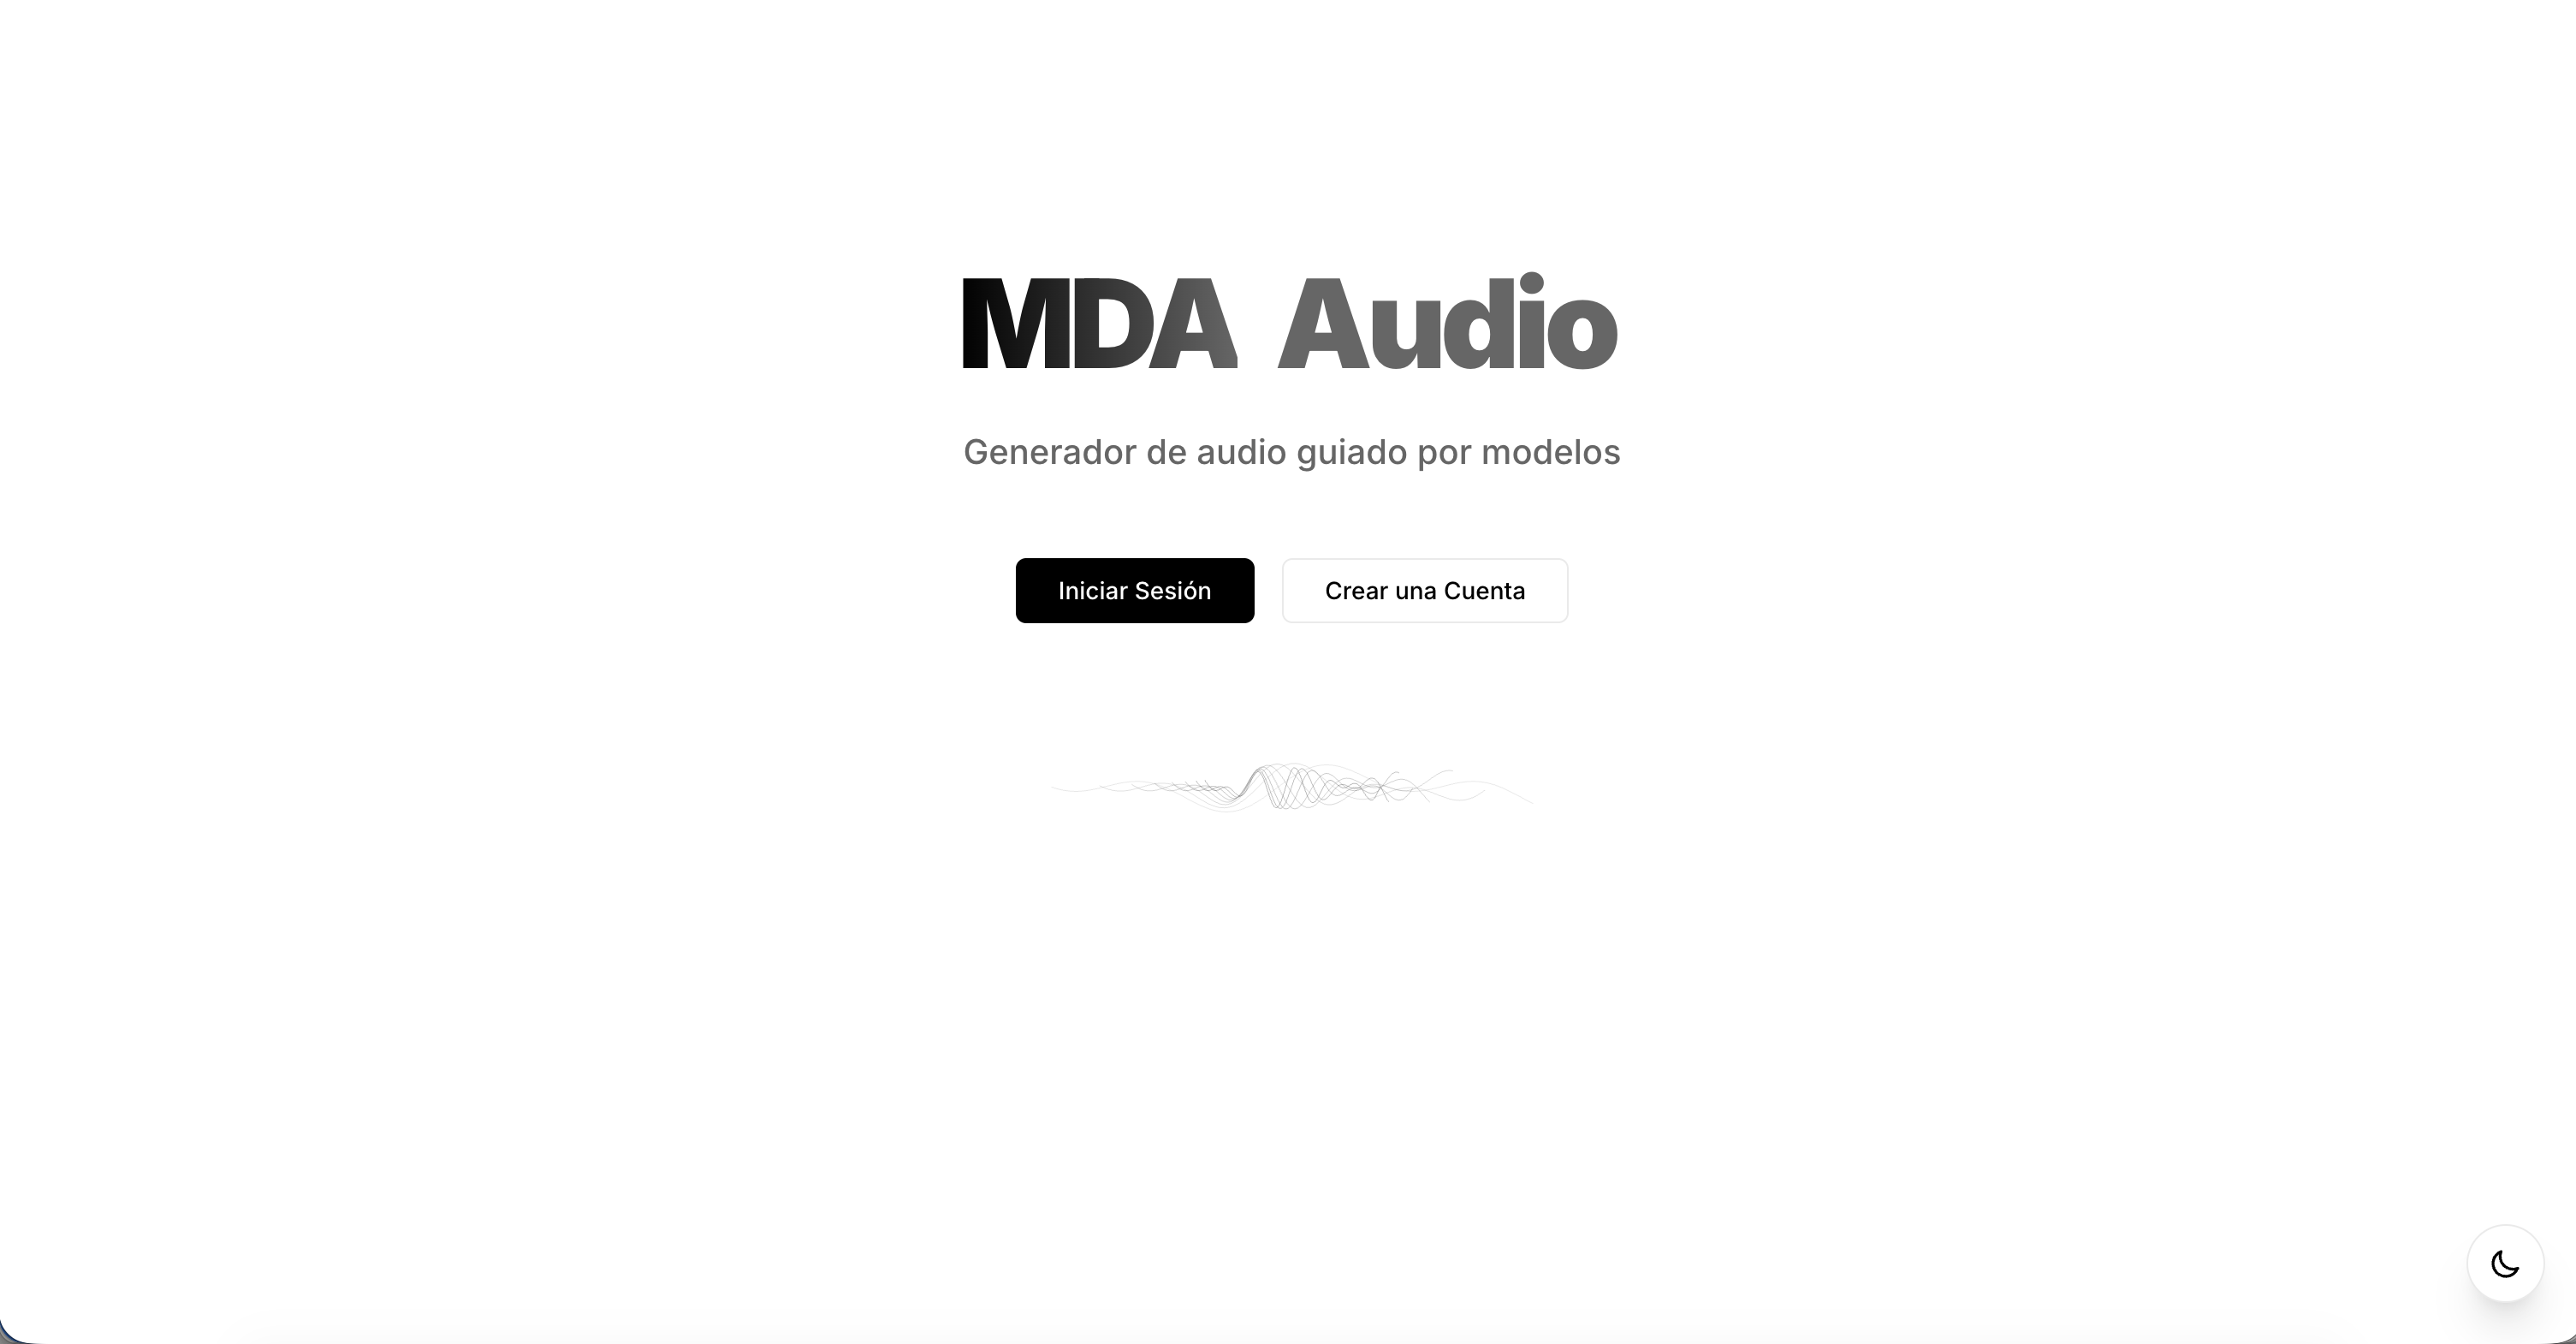
\includegraphics[width=\textwidth]{imagenes/01_inicio/01_pantallaInicioBlanca.png}
    \caption{Pantalla de inicio en tema claro.}
\end{figure}

Esta interfaz muestra una disposición limpia, diseñada para orientar rápidamente al usuario sobre las capacidades del sistema. Las opciones disponibles en esta vista inicial son:

\begin{itemize}
    \item \textbf{Barra de navegación superior:} Contiene el título de la aplicación y botones de acceso rápido para iniciar sesión o registrarse en el sistema.
    \item \textbf{Área de contenido principal:} Muestra información introductoria y llamadas a la acción para comenzar a trabajar con los modelos \textit{CIM} y \textit{PIM}.
\end{itemize}

\begin{figure}[!ht]
    \centering
    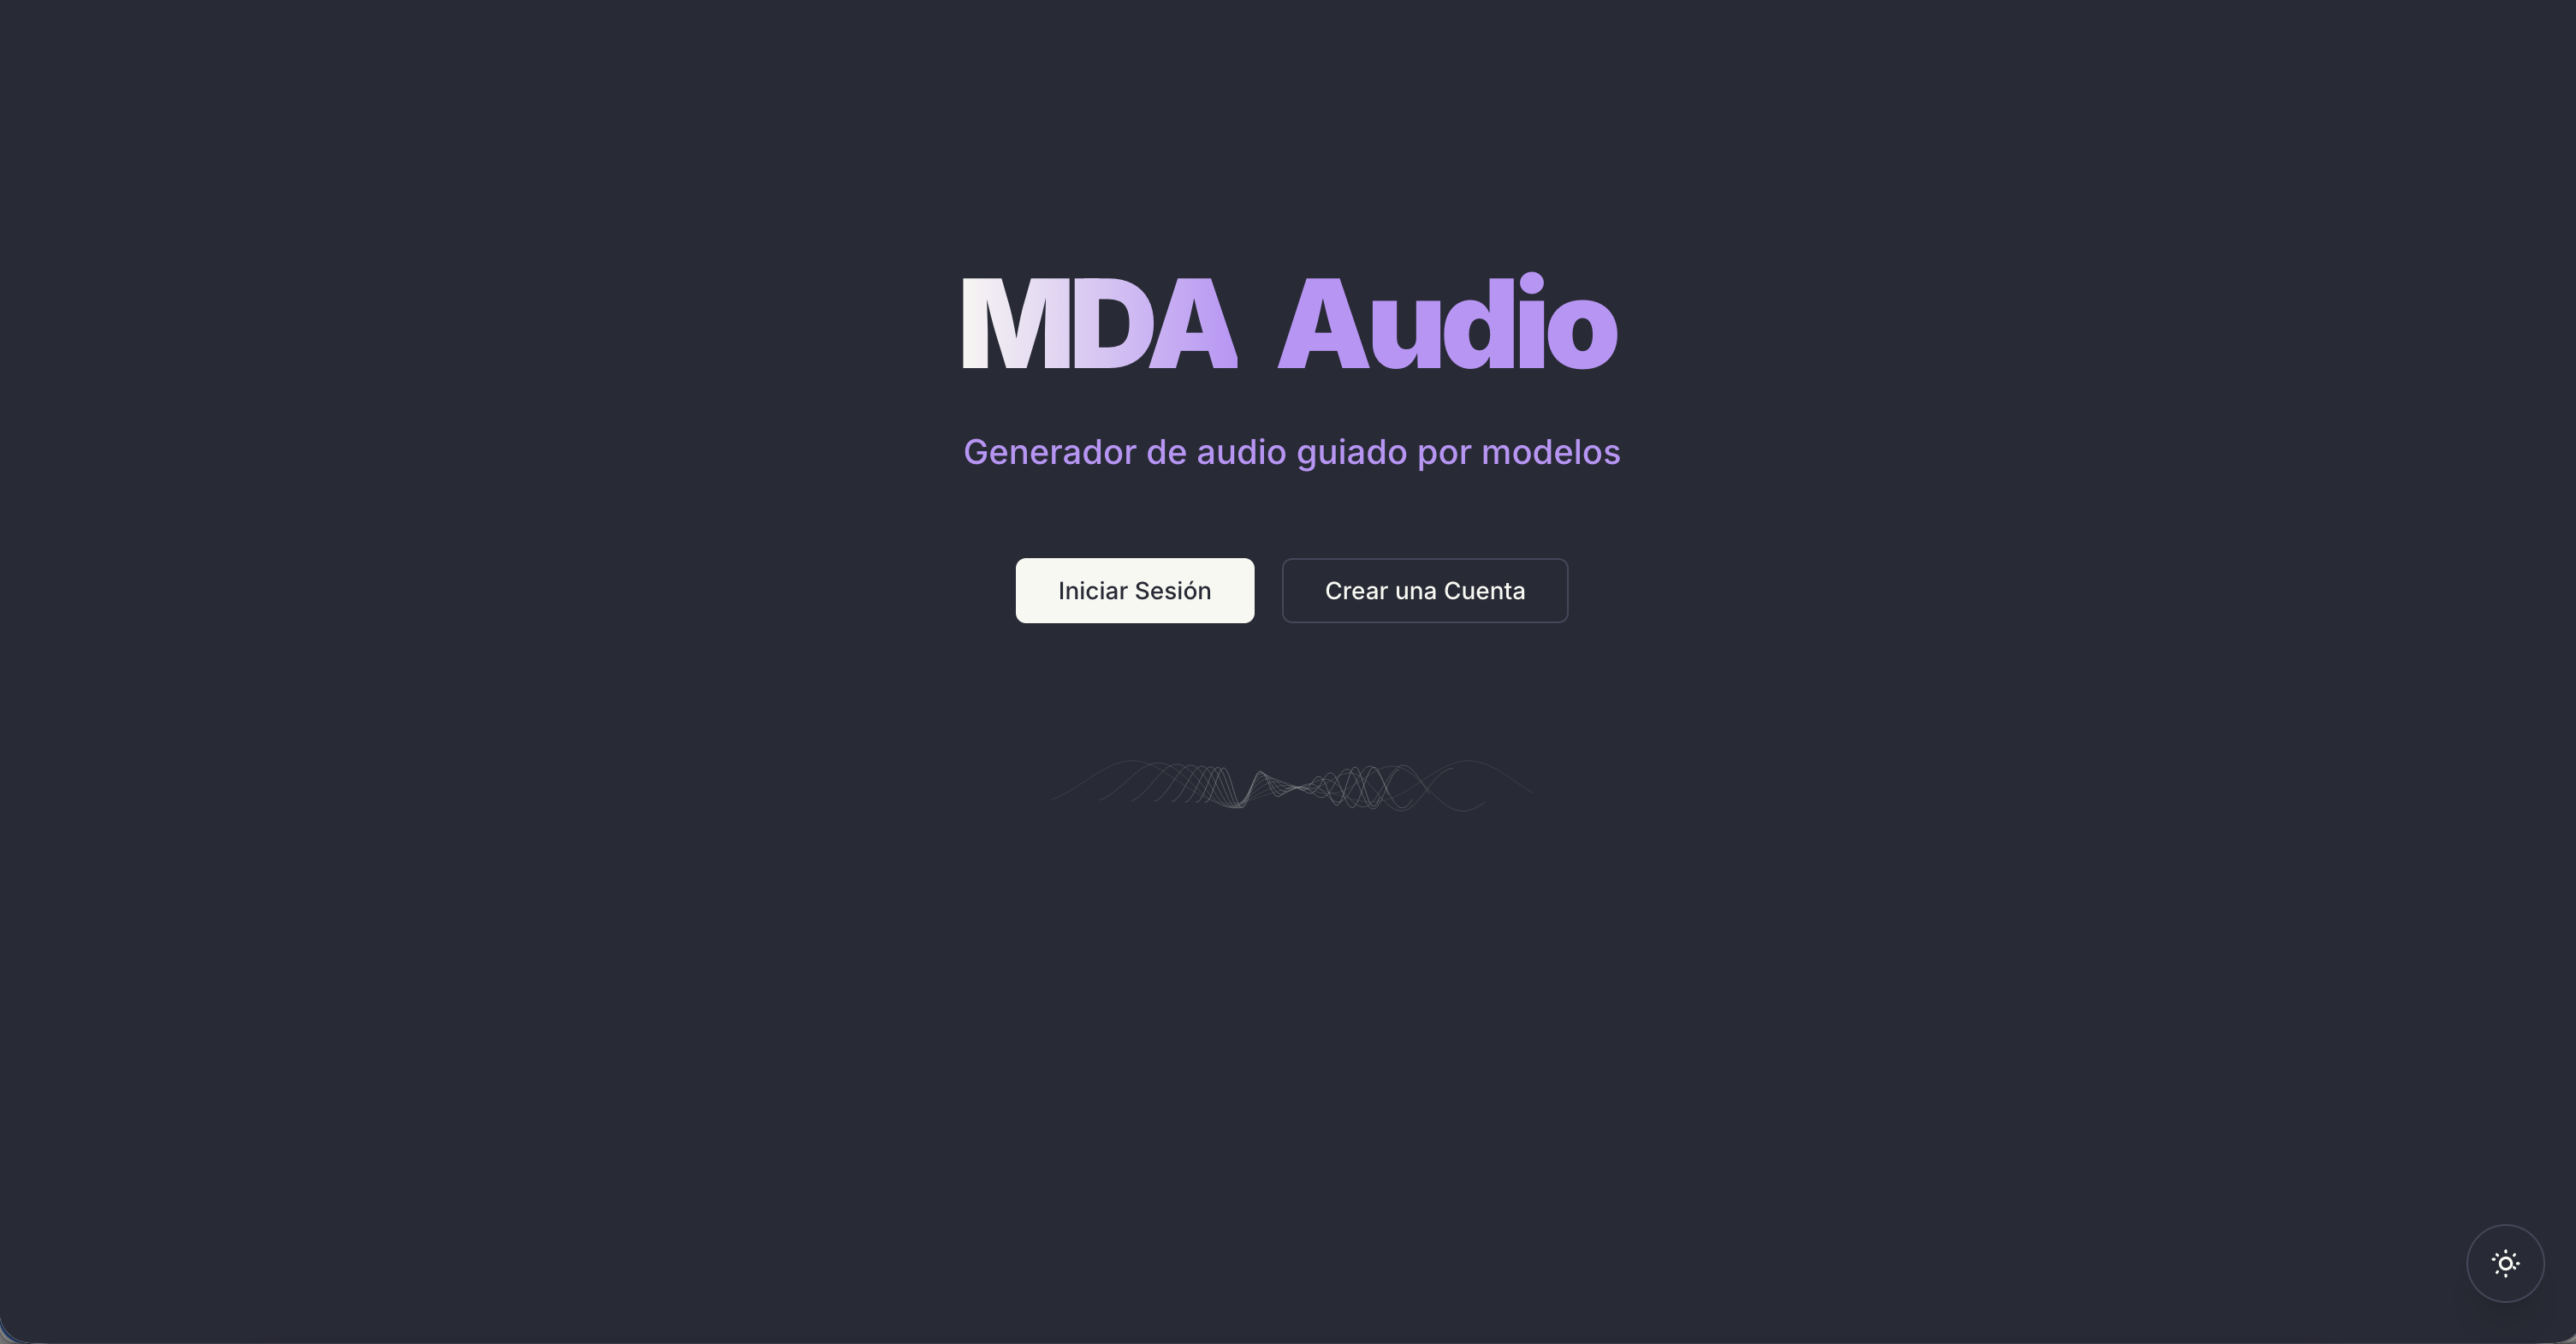
\includegraphics[width=\textwidth]{imagenes/01_inicio/02_pantallaInicioOscura.png}
    \caption{Pantalla de inicio en tema oscuro.}
\end{figure}

La aplicación soporta de forma nativa la alternancia de temas. El tema oscuro reduce la fatiga visual y puede ser activado según las preferencias del sistema operativo del usuario. Las funcionalidades, accesos y opciones de la pantalla son completamente idénticas a las del tema claro.

\chapter{Gestión de Usuarios y Acceso}

\section{Registro e Inicio de Sesión}

Para comenzar a utilizar las funcionalidades de \textit{MDAA}, es necesario disponer de una cuenta de usuario. La aplicación gestiona la autenticación de manera segura, permitiendo registrar nuevos usuarios e iniciar sesión a aquellos que ya poseen credenciales.

\begin{figure}[!ht]
    \centering
    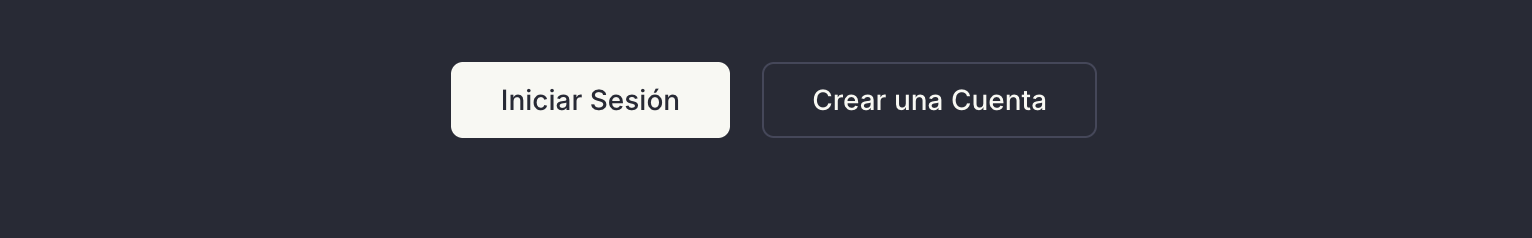
\includegraphics[width=0.5\textwidth]{imagenes/02_usuario/01_botoneraLoginORegistro.png}
    \caption{Botonera de acceso y registro en la barra superior.}
\end{figure}

En la parte superior derecha de la pantalla de inicio, se encuentran las opciones de acceso. El usuario puede:
\begin{itemize}
    \item \textbf{Iniciar Sesión:} Si ya dispone de una cuenta verificada.
    \item \textbf{Registrarse:} Para crear una nueva cuenta y poder acceder a la creación de proyectos.
\end{itemize}

\subsection{Creación de un Nuevo Usuario}

Al seleccionar la opción de registro, se presenta un formulario de creación de cuenta. Es vital proporcionar datos precisos, especialmente el correo electrónico, ya que se requerirá su verificación.

\begin{figure}[!ht]
    \centering
    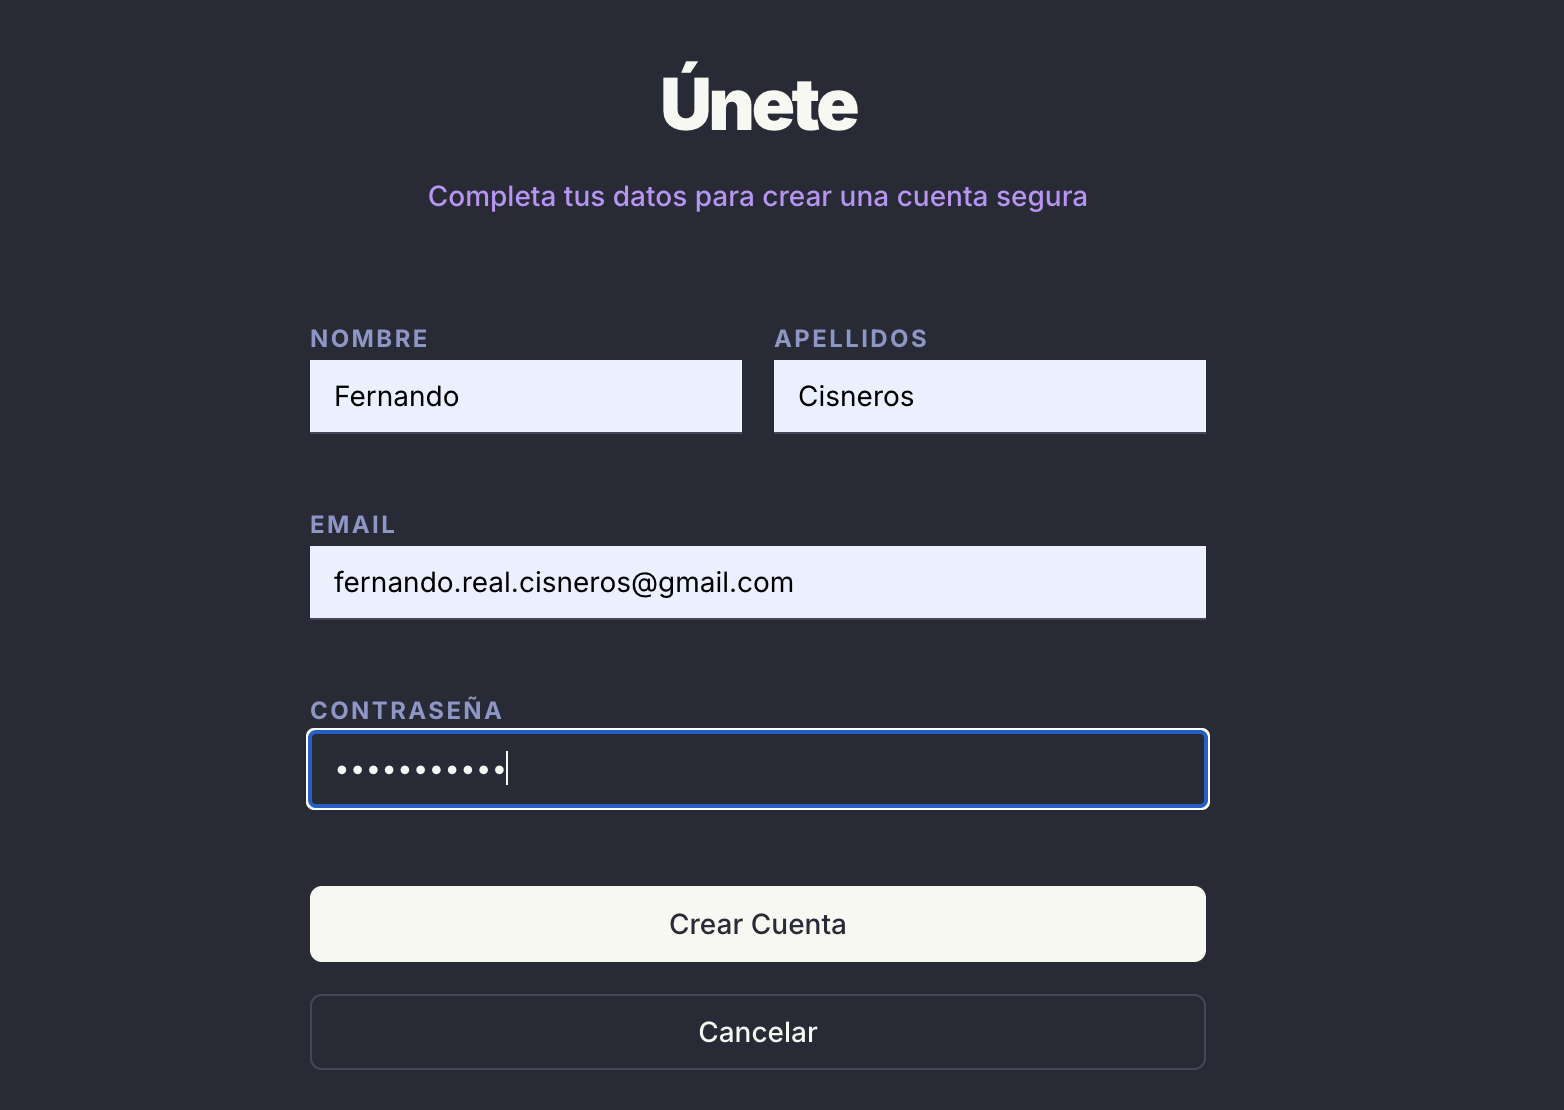
\includegraphics[width=0.6\textwidth]{imagenes/02_usuario/03_creacionDeUsuario.png}
    \caption{Formulario de registro de usuario.}
\end{figure}

El formulario requiere rellenar los siguientes campos:
\begin{itemize}
    \item \textbf{Nombre:} Nombre de pila del usuario.
    \item \textbf{Apellidos:} Apellidos del usuario.
    \item \textbf{Correo electrónico:} Dirección válida que servirá como identificador único y medio para verificar la cuenta.
    \item \textbf{Contraseña:} Credencial secreta. Debe cumplir con criterios mínimos de seguridad.
    \item \textbf{Confirmación de contraseña:} Para asegurar que no hay errores tipográficos.
\end{itemize}

\begin{figure}[!ht]
    \centering
    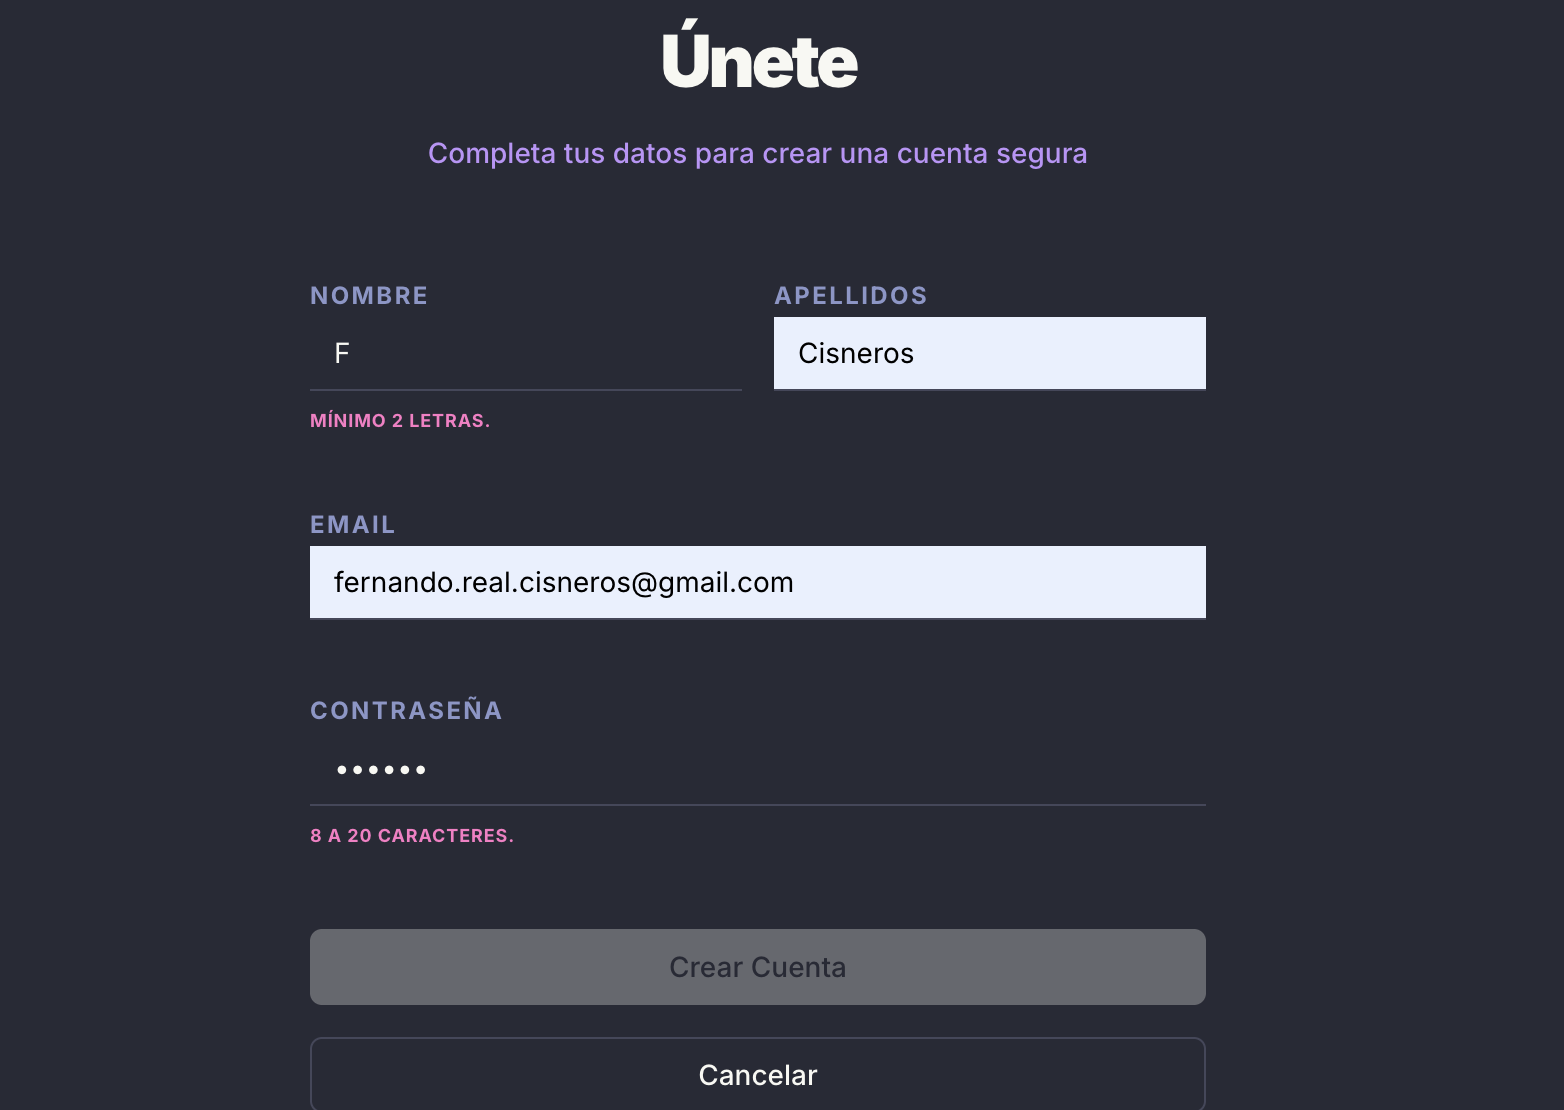
\includegraphics[width=0.6\textwidth]{imagenes/02_usuario/02_validacionRegistroNuevoUsuario.png}
    \caption{Validación de campos en el formulario de registro.}
\end{figure}

Si los datos introducidos no cumplen los requisitos (por ejemplo, correos electrónicos mal formateados o contraseñas que no coinciden), la aplicación mostrará alertas de validación, impidiendo el registro hasta que se corrijan los errores.

\begin{figure}[!ht]
    \centering
    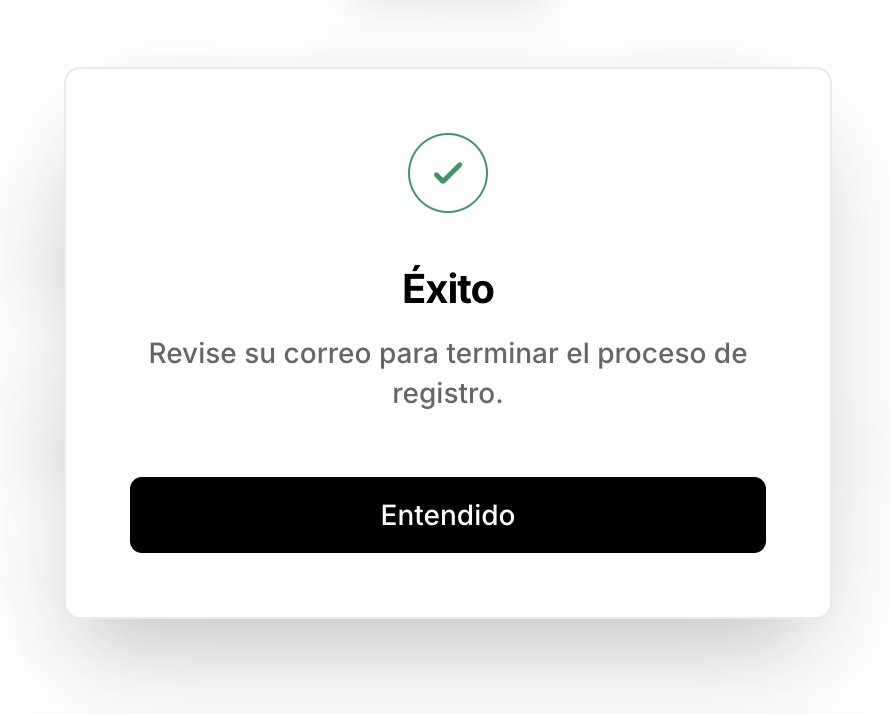
\includegraphics[width=0.6\textwidth]{imagenes/02_usuario/04_CreacionConExitoDeNuevoUsuario.png}
    \caption{Mensaje de éxito tras el registro y aviso de verificación de correo.}
\end{figure}

Tras enviar el formulario correctamente, la aplicación notifica que la cuenta ha sido creada y que es imperativo verificar la dirección de correo electrónico antes de poder iniciar sesión por primera vez.

\subsection{Verificación de Correo Electrónico}

En entornos de desarrollo y pruebas, el sistema captura los correos electrónicos enviados a través de una herramienta integrada (\textit{MailHog}).

\begin{figure}[!ht]
    \centering
    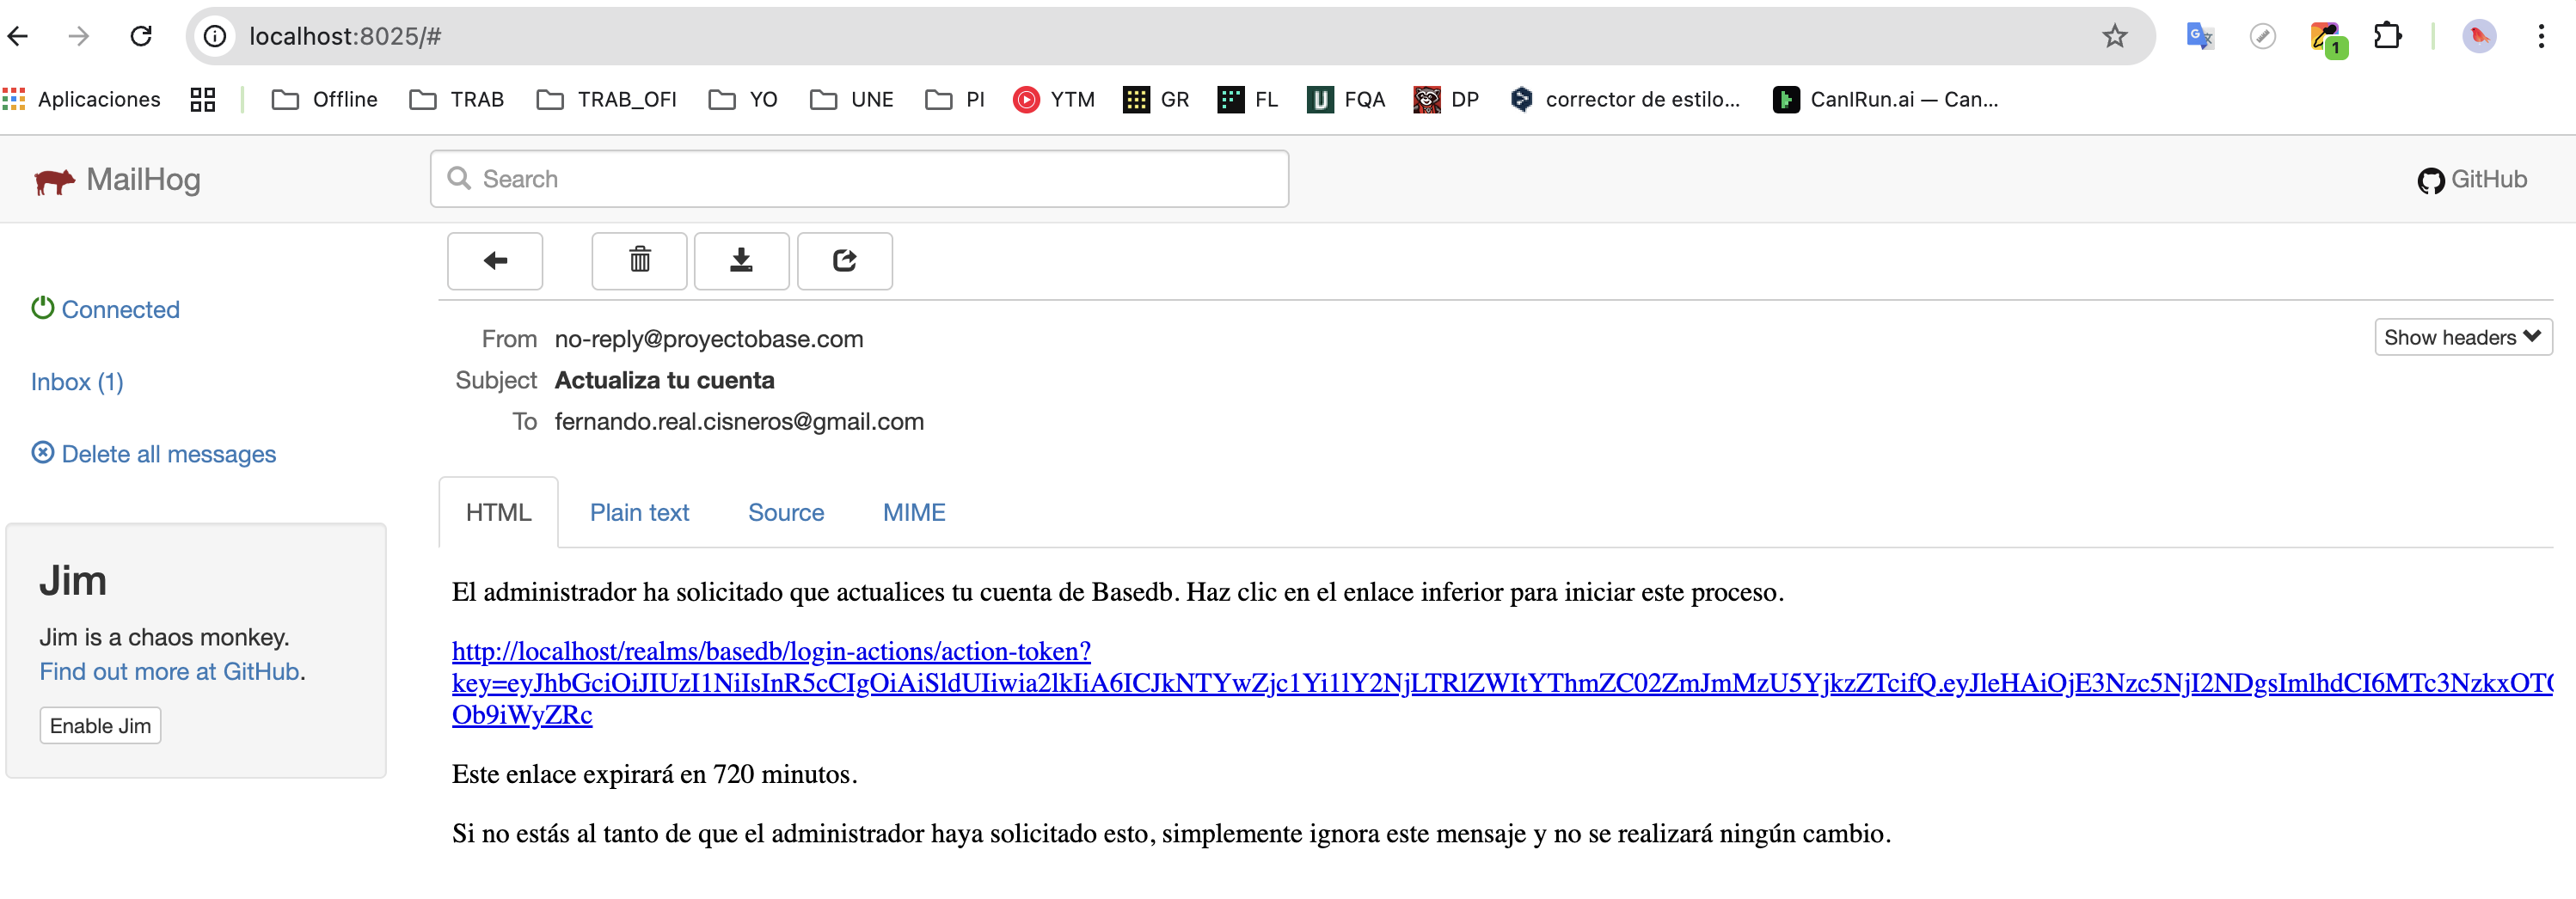
\includegraphics[width=\textwidth]{imagenes/02_usuario/05_verificarMailConElEntornoDeDesarrolloMailHog.png}
    \caption{Buzón de correo simulado para verificar la cuenta.}
\end{figure}

\begin{figure}[!ht]
    \centering
    
\includegraphics[width=0.6\textwidth]{imagenes/02_usuario/06_linkDeVerificarEnKeyCloak.png}
    \caption{Enlace de verificación de correo electrónico.}
\end{figure}

Al abrir el correo recibido, el usuario debe pulsar el enlace proporcionado para confirmar que es el propietario de la dirección indicada. Este paso interactúa directamente con el sistema de seguridad subyacente.

\begin{figure}[!ht]
    \centering
    
\includegraphics[width=0.6\textwidth]{imagenes/02_usuario/07_linkDeVolverAAplicacion.png}
    \caption{Confirmación de correo electrónico verificado.}
\end{figure}

\begin{figure}[!ht]
    \centering
    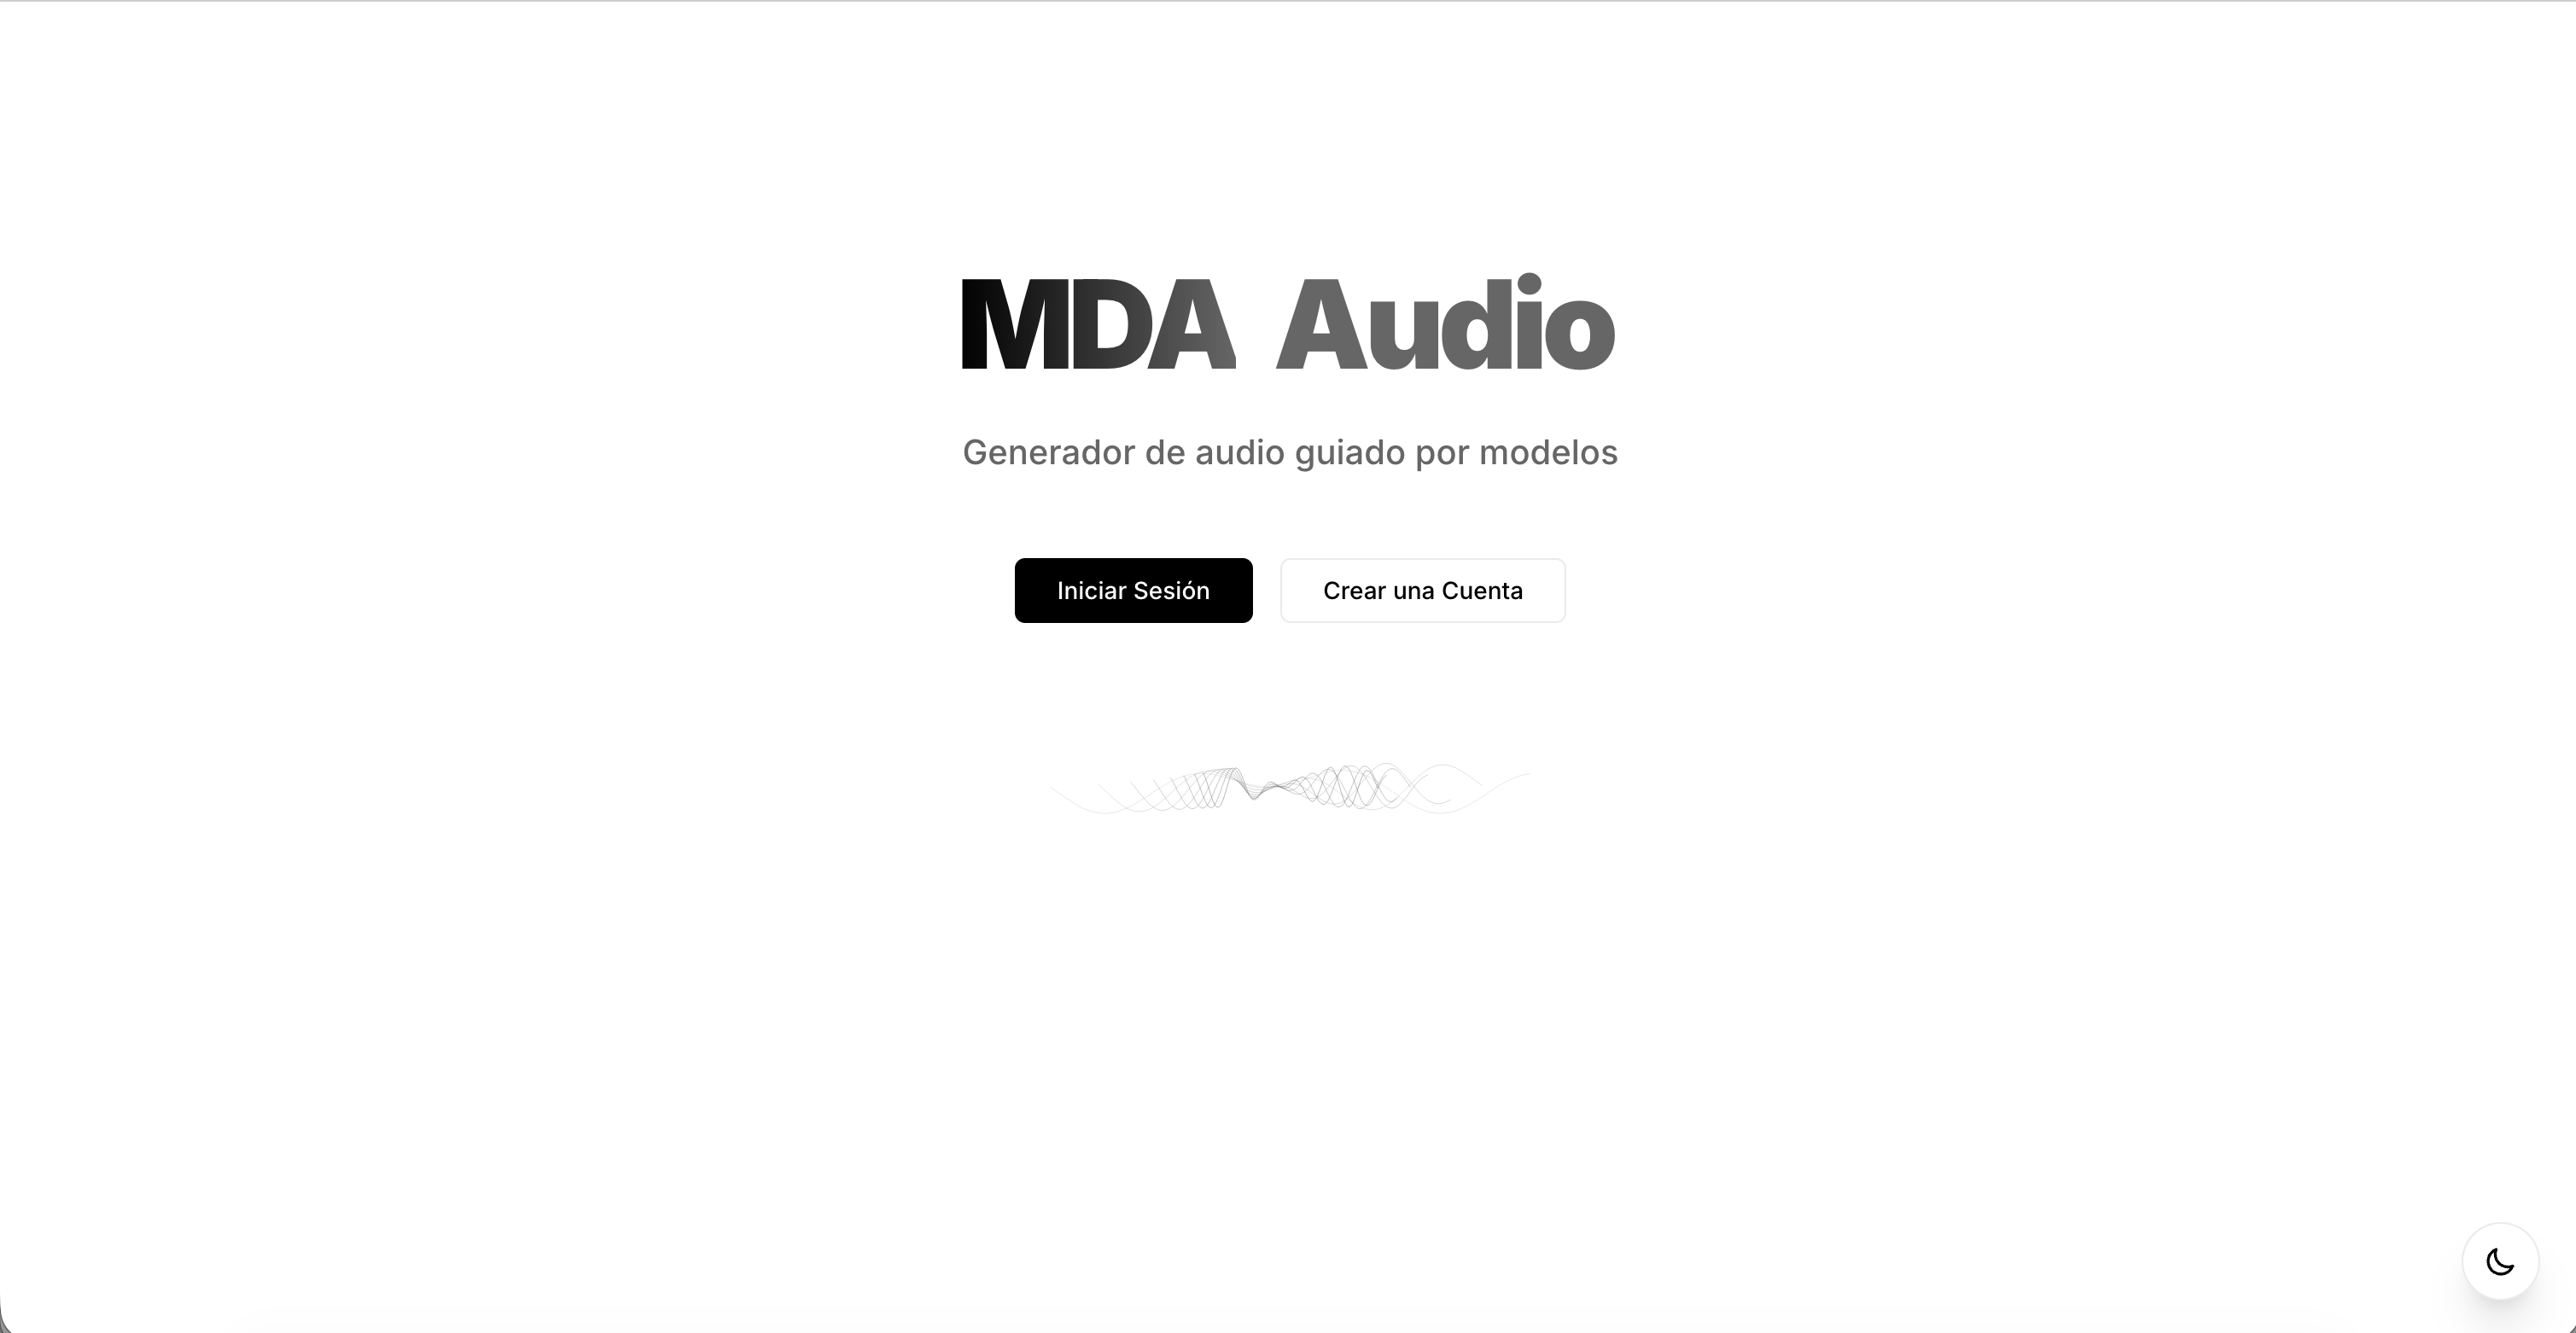
\includegraphics[width=0.6\textwidth]{imagenes/02_usuario/09_volverAAplicacion.png}
    \caption{Enlace para volver a la aplicación tras la verificación.}
\end{figure}

Una vez verificada la cuenta, se mostrará un mensaje de confirmación y un enlace directo para regresar a la aplicación \textit{MDAA} y proceder al inicio de sesión.

\subsection{Inicio de Sesión y Acceso}

Con la cuenta verificada, el usuario ya puede autenticarse.

\begin{figure}[!ht]
    \centering
    
\includegraphics[width=0.5\textwidth]{imagenes/02_usuario/10_botonInicioSesion.png}
    \caption{Botón de inicio de sesión.}
\end{figure}

Al pulsar el botón de iniciar sesión desde la pantalla principal, se redirige al usuario a la pasarela segura.

\begin{figure}[!ht]
    \centering
    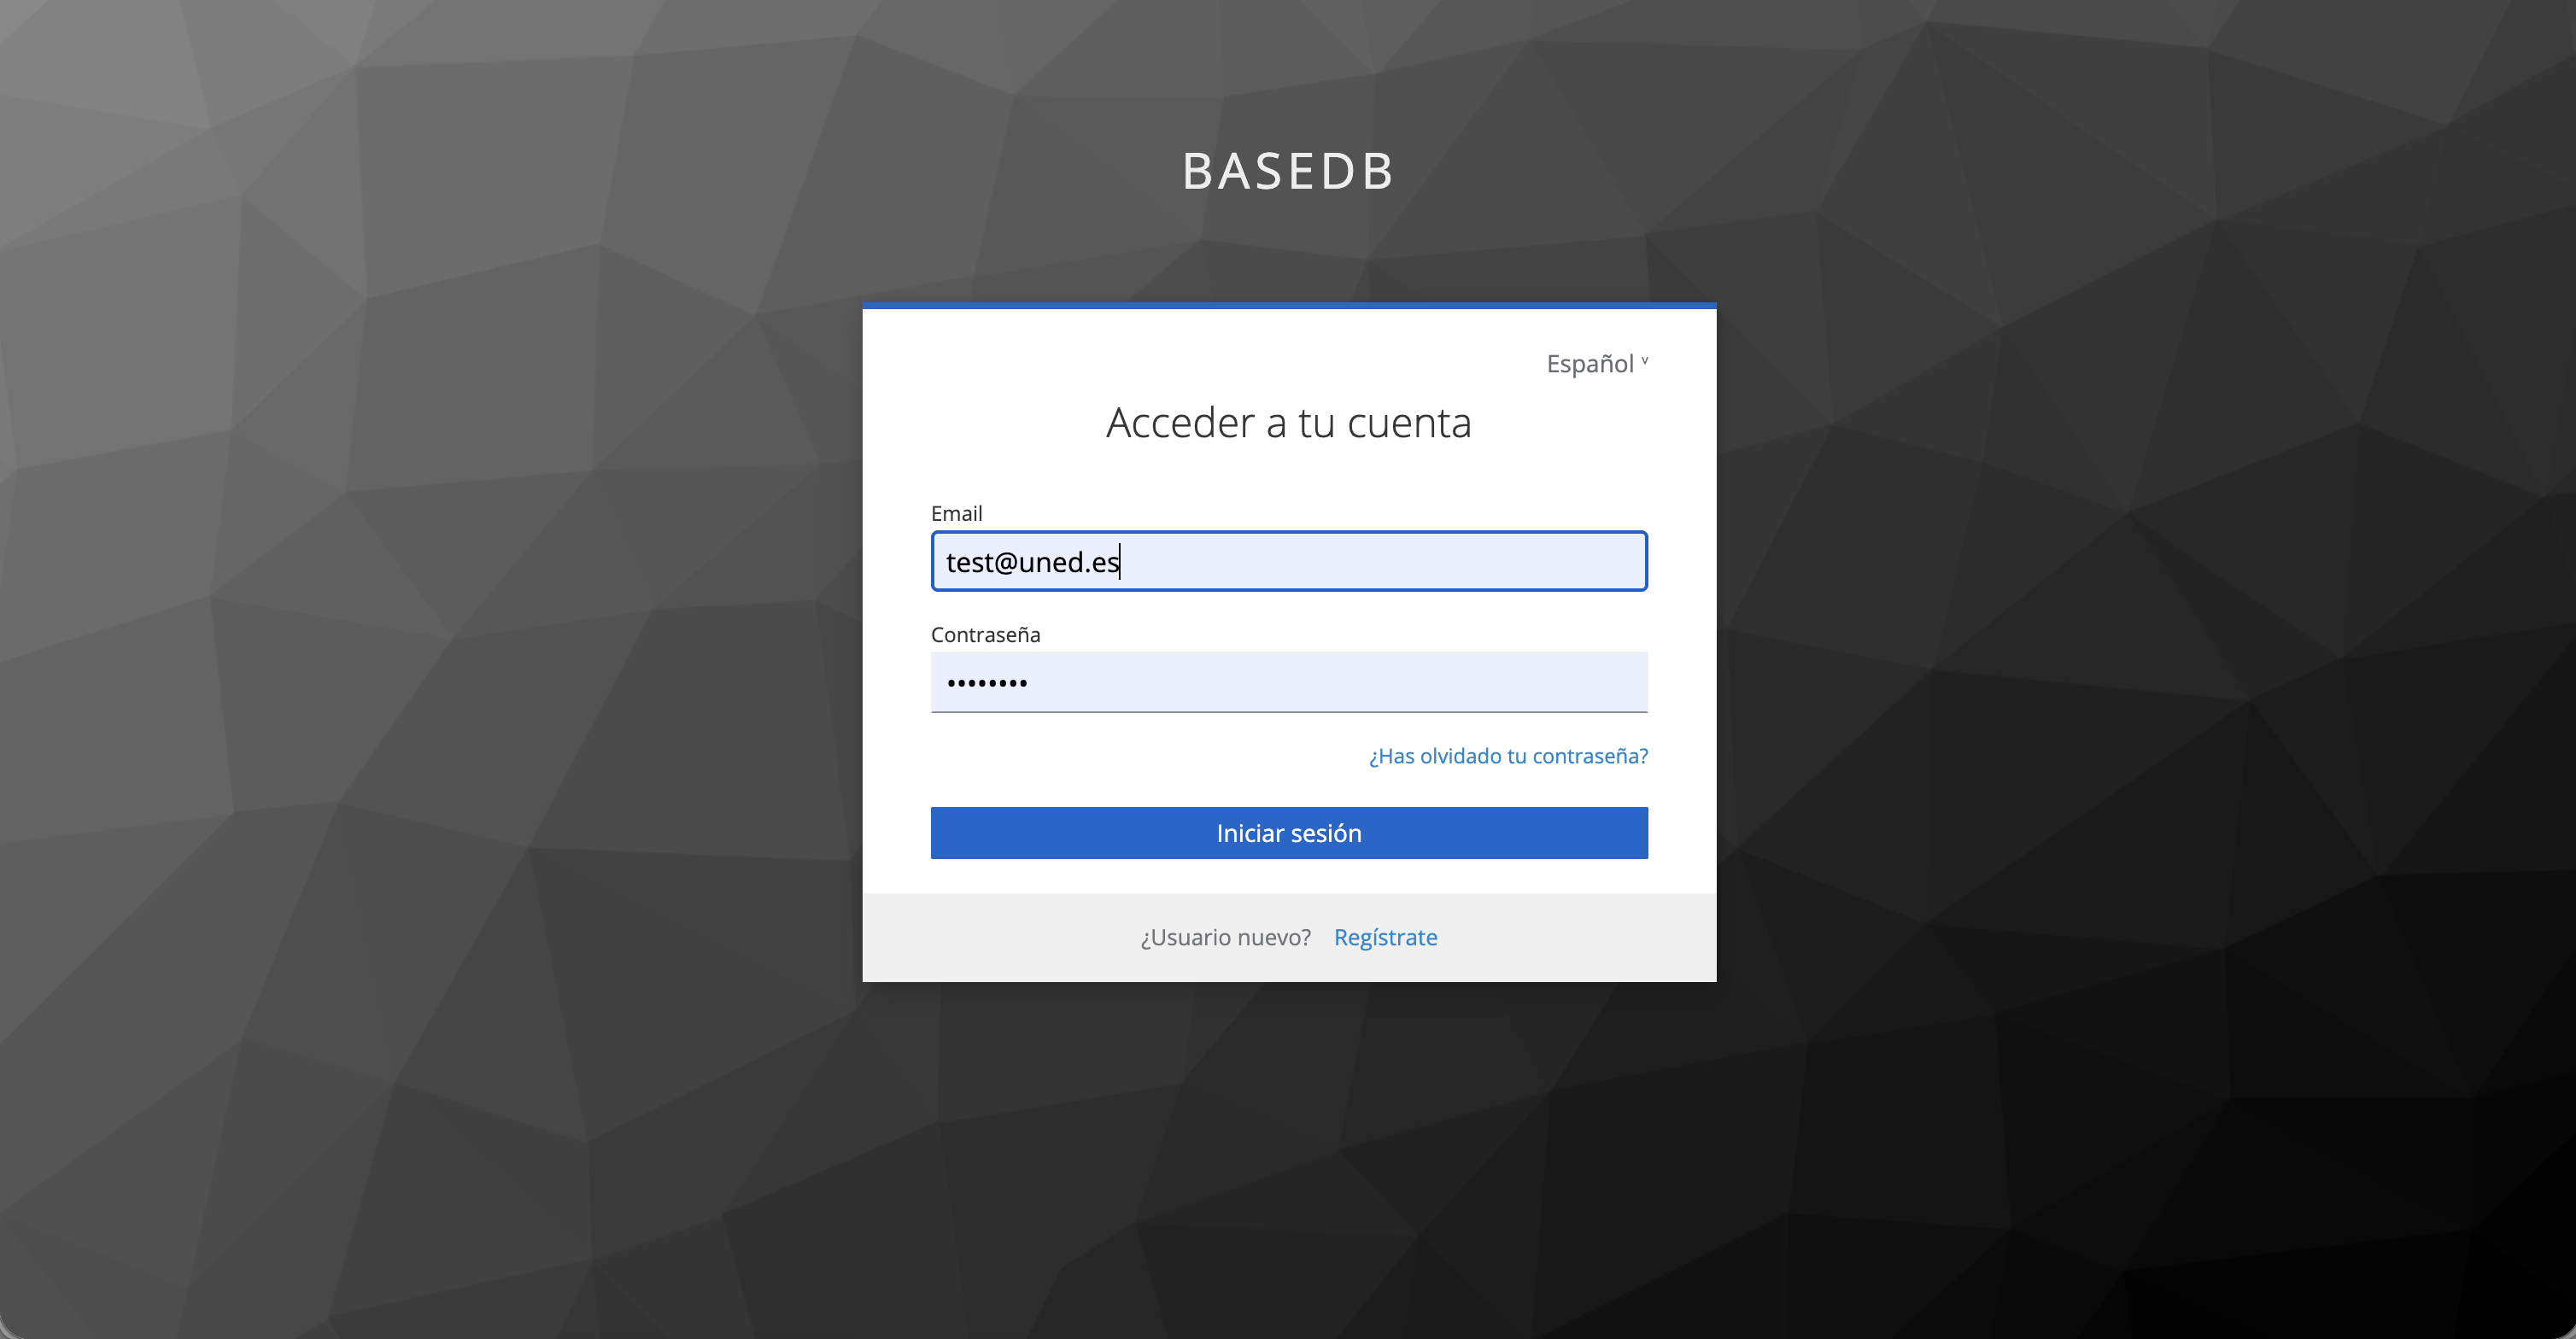
\includegraphics[width=0.6\textwidth]{imagenes/02_usuario/11_loginConUsarioTestQueDebemosUtilizarParaProbar.png}
    \caption{Formulario de inicio de sesión con usuario de pruebas.}
\end{figure}

En este formulario, se deben introducir:
\begin{itemize}
    \item \textbf{Usuario o correo electrónico:} Identificador registrado. Para pruebas se puede utilizar un usuario preconfigurado (\textit{test}).
    \item \textbf{Contraseña:} La clave asociada a la cuenta.
    \item \textbf{Opciones adicionales:} Enlaces para recuperar contraseñas olvidadas si estuviesen configuradas.
\end{itemize}

\begin{figure}[!ht]
    \centering
    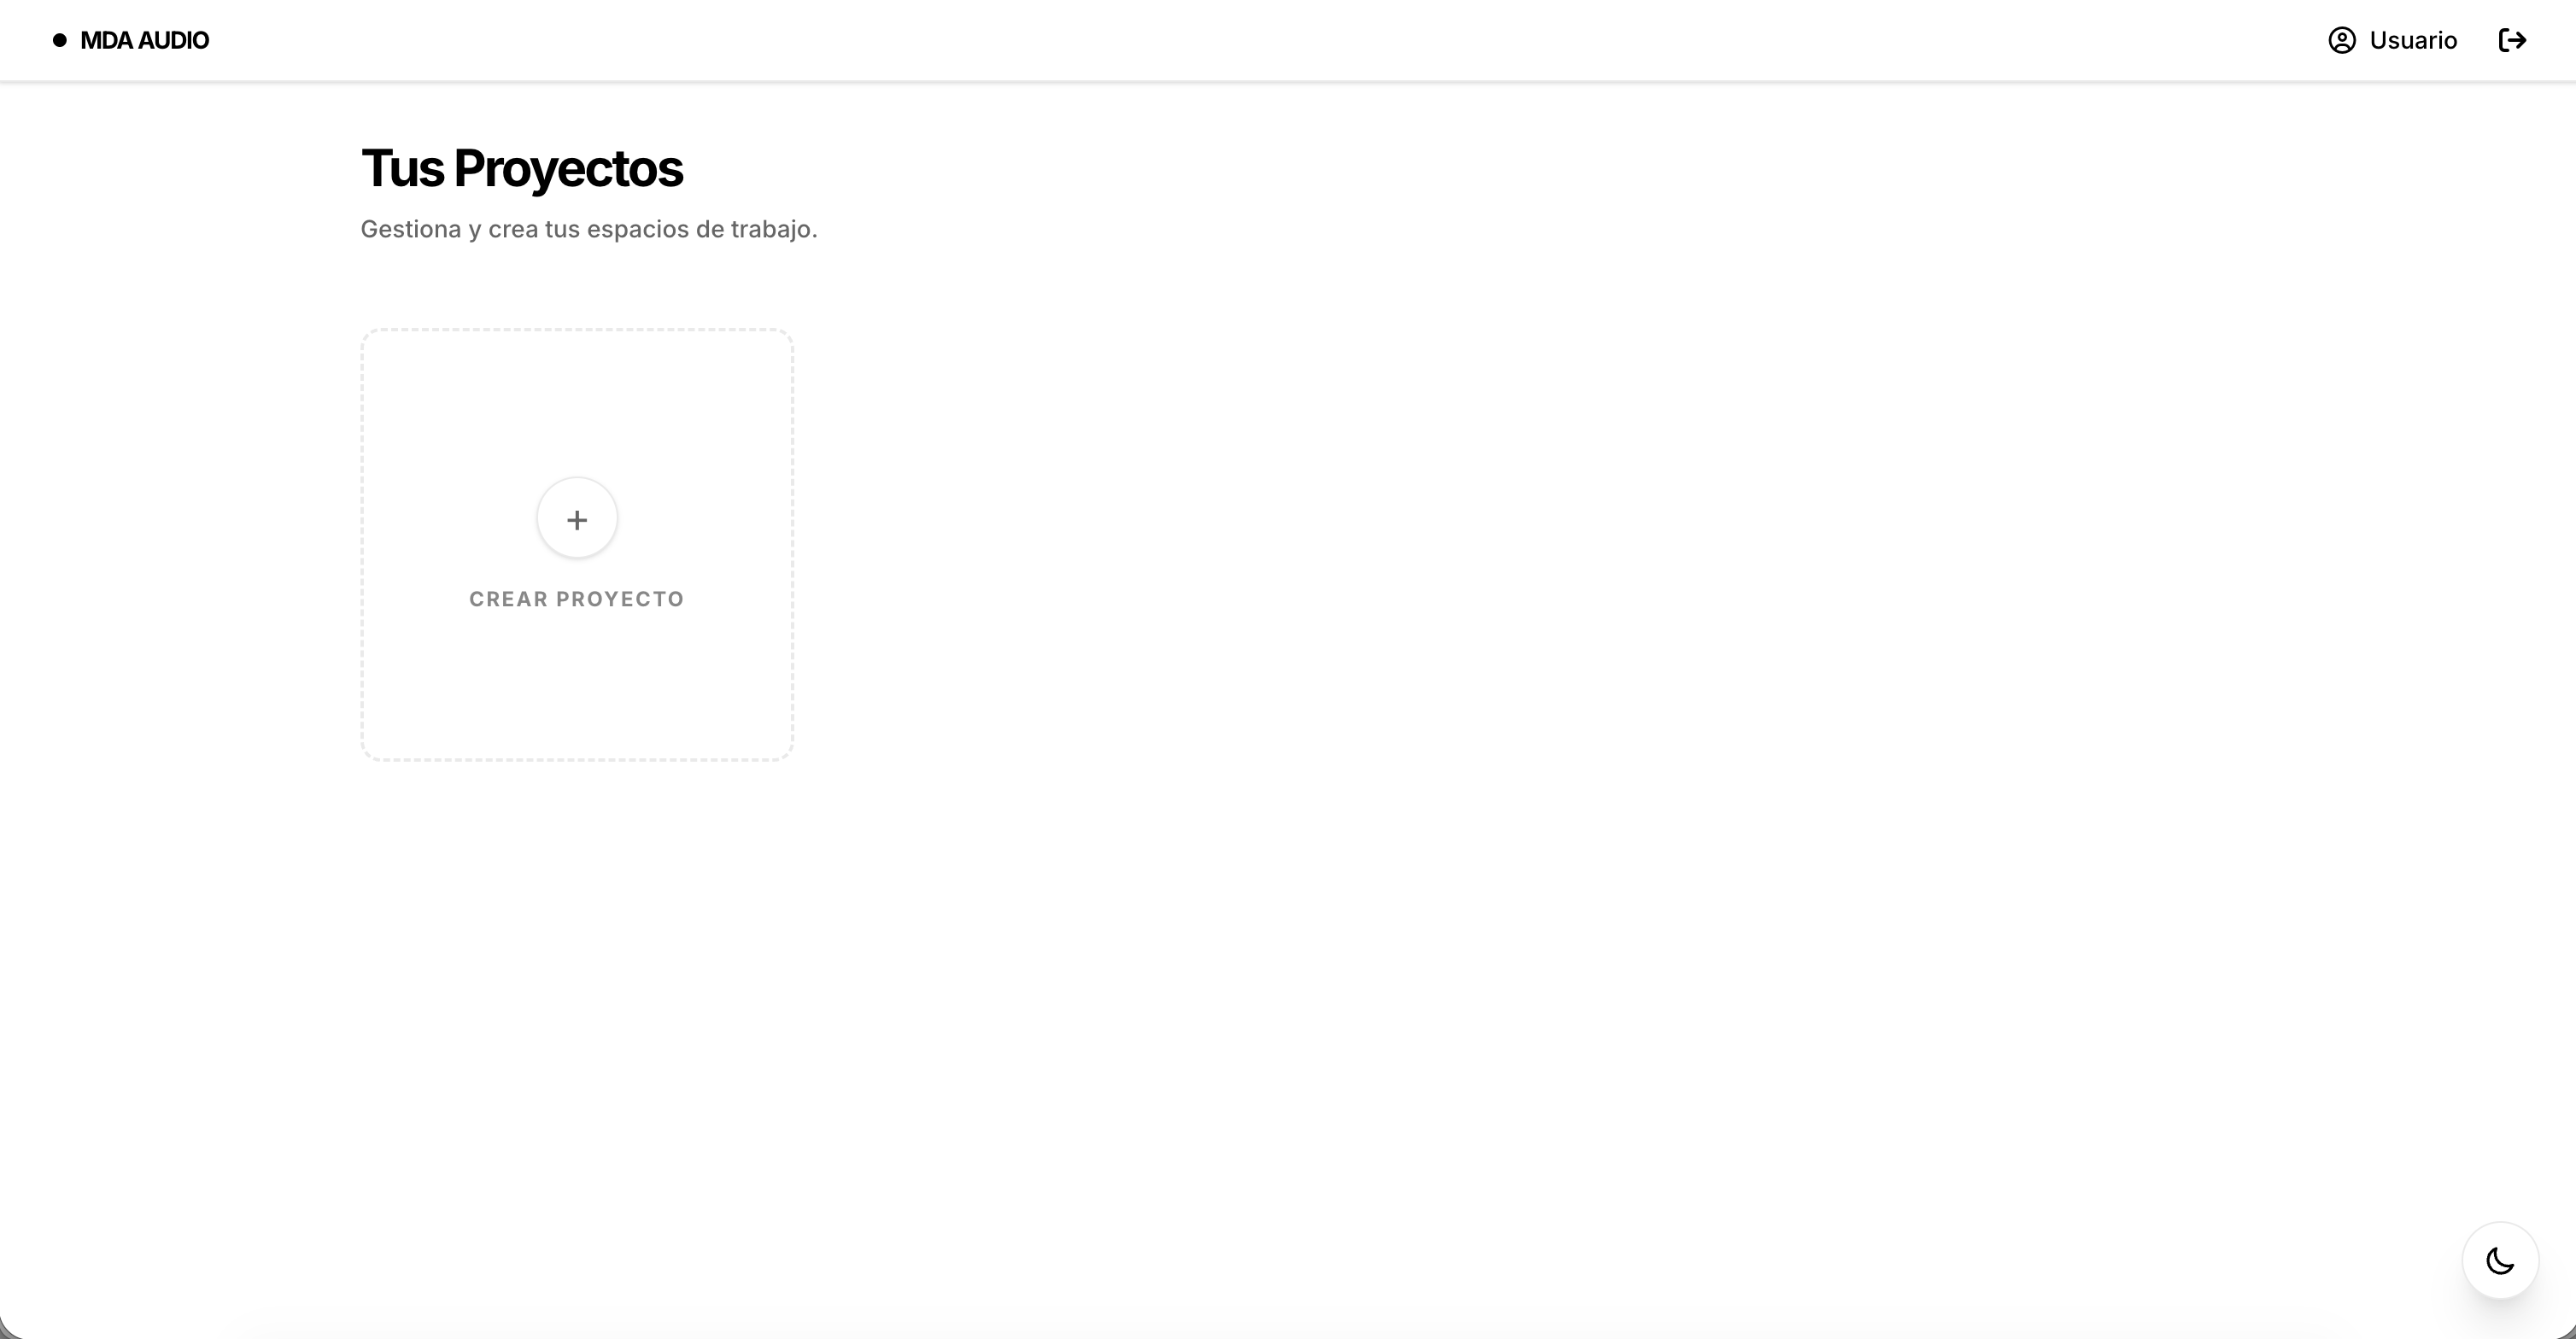
\includegraphics[width=\textwidth]{imagenes/02_usuario/12_entradaEnLaAplicacion.png}
    \caption{Pantalla principal tras iniciar sesión exitosamente.}
\end{figure}

Si las credenciales son correctas, el sistema autentica al usuario y le redirige a su área de trabajo personal, donde se listan sus proyectos y se habilita la interacción con los módulos de generación de código y validación \textit{DSL}.

\chapter{Gestión de Proyectos}

\section{Panel Principal de Proyectos}

Una vez que el usuario ha iniciado sesión, accede a su panel de control o área de trabajo. En esta pantalla se centraliza la gestión de todos los proyectos creados. Un proyecto agrupa todos los modelos, configuraciones y elementos necesarios para definir sintetizadores de audio utilizando el lenguaje de dominio.

\begin{figure}[!ht]
    \centering
    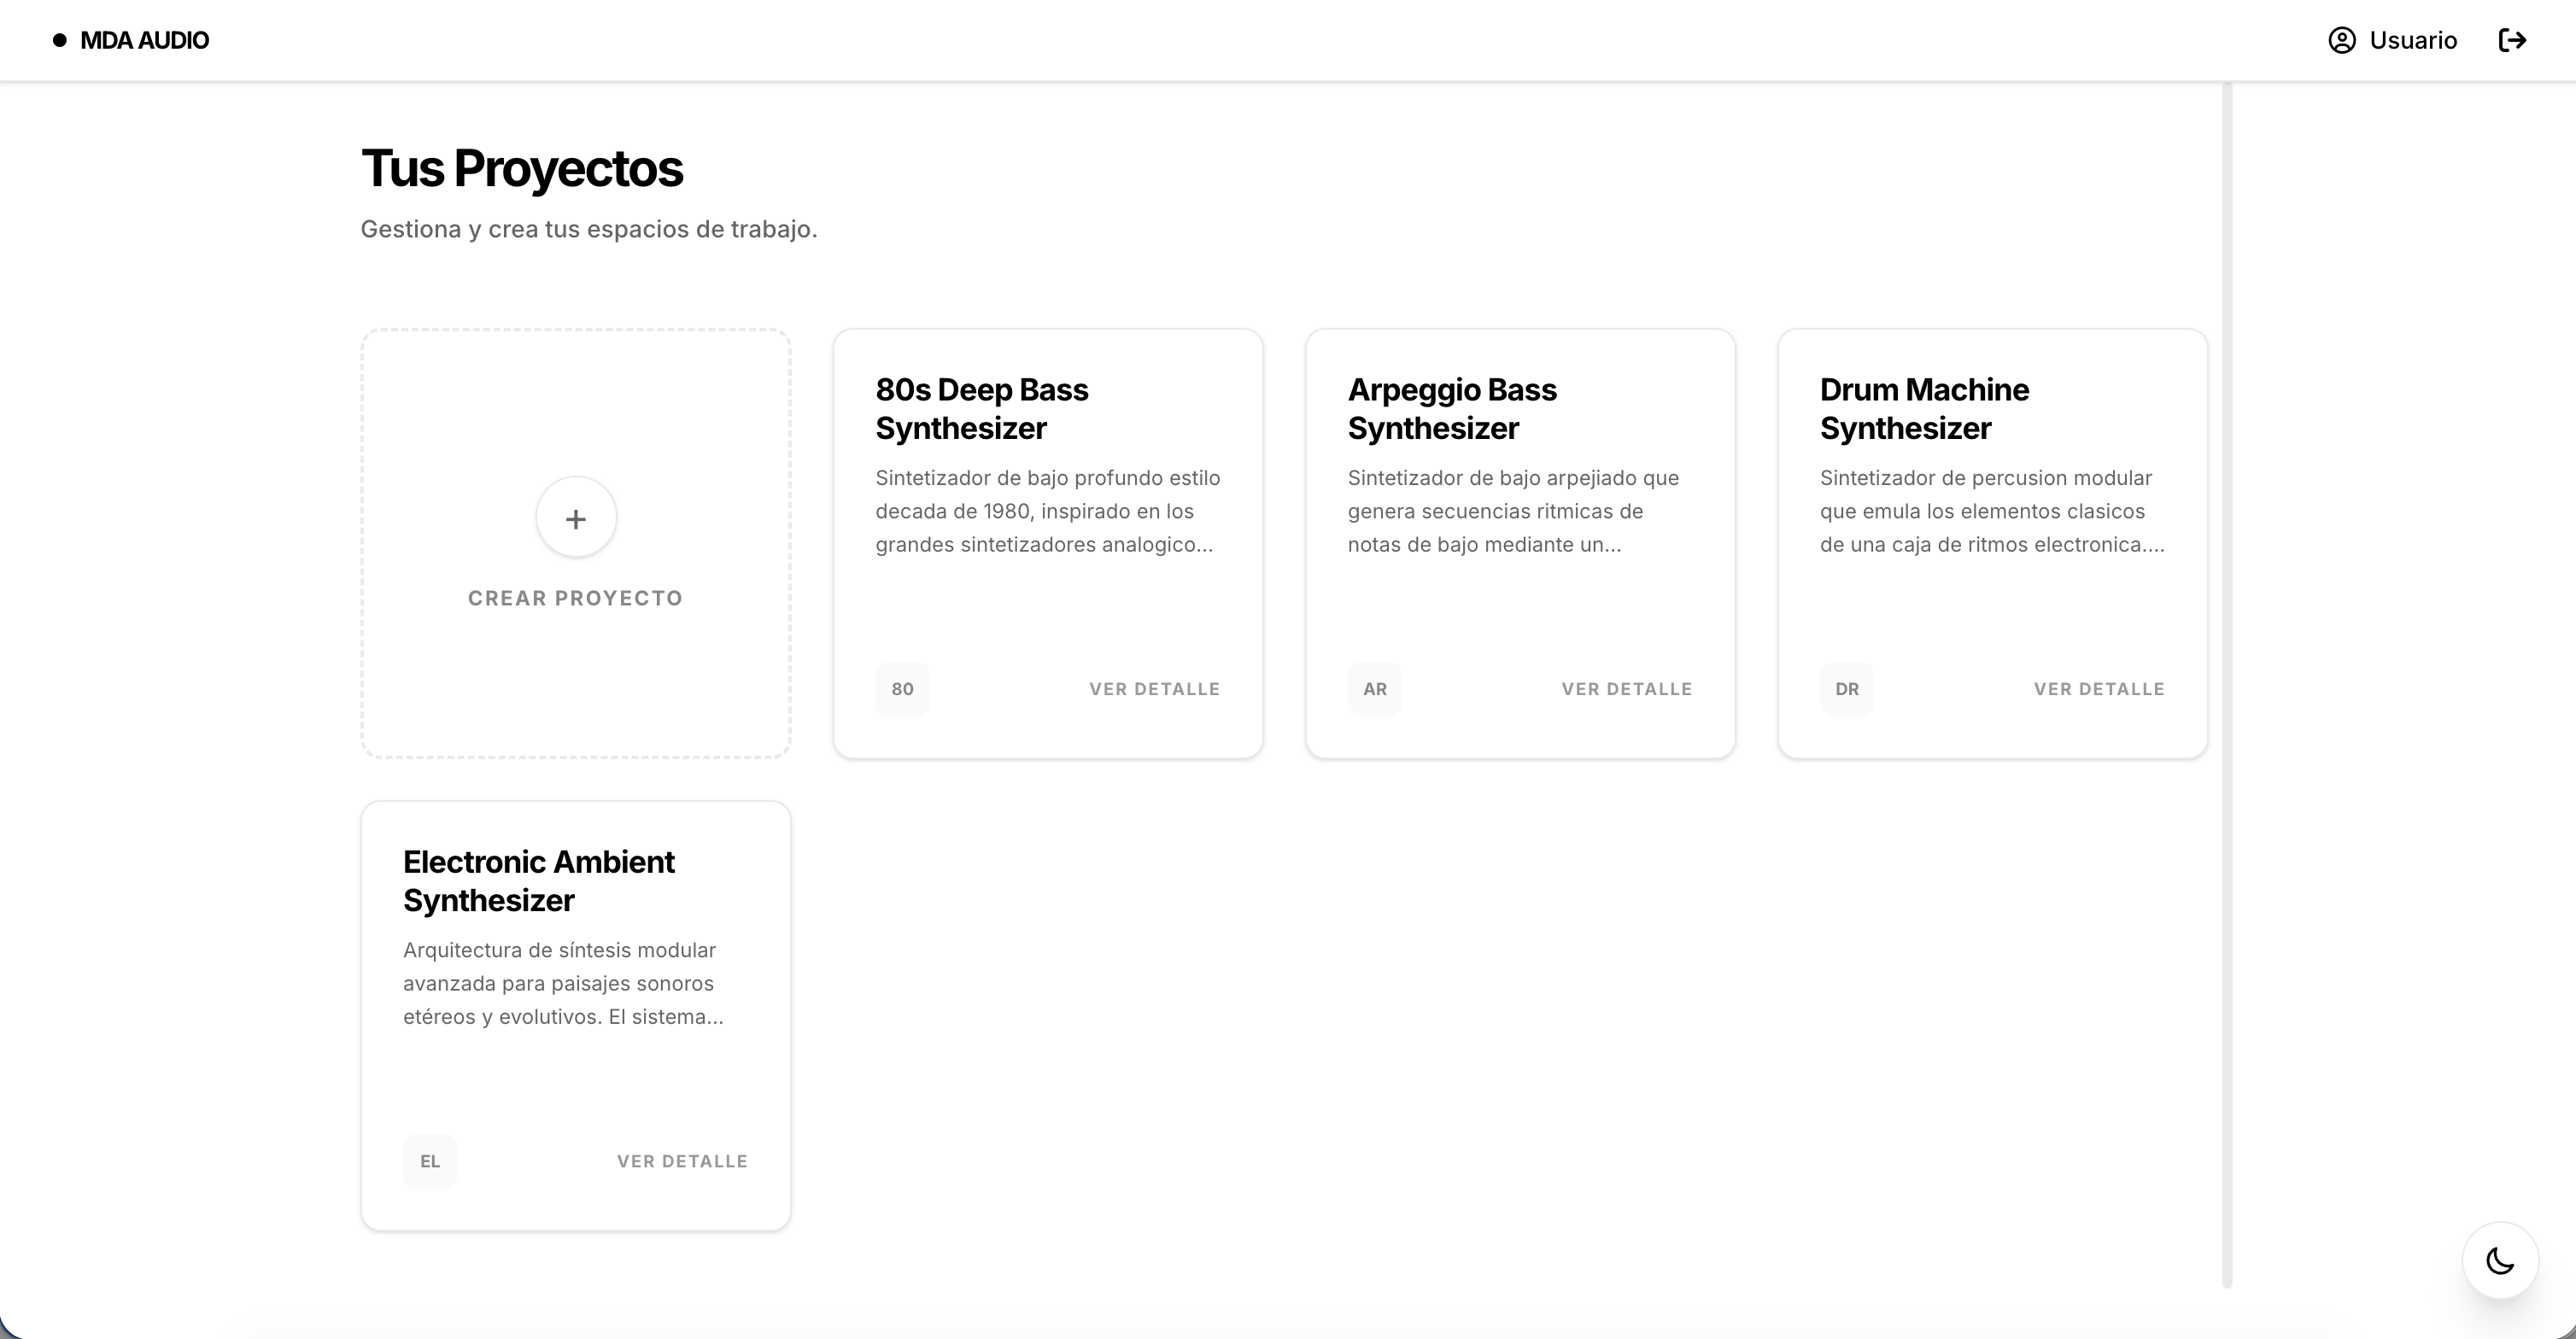
\includegraphics[width=\textwidth]{imagenes/03_proyecto/01_vistaPrincipalConLosProyectos.png}
    \caption{Vista principal con el listado de proyectos.}
\end{figure}

El panel principal ofrece las siguientes capacidades:
\begin{itemize}
    \item \textbf{Visualización de Proyectos:} Cada proyecto se muestra como una tarjeta que incluye su nombre, un color identificativo y un resumen de su contenido o estado.
    \item \textbf{Creación de Nuevos Proyectos:} Botón dedicado para añadir un nuevo elemento al espacio de trabajo.
    \item \textbf{Gestión de la Sesión:} Controles de usuario situados en la barra superior.
\end{itemize}

\subsection{Creación de un Proyecto}

\begin{figure}[!ht]
    \centering
    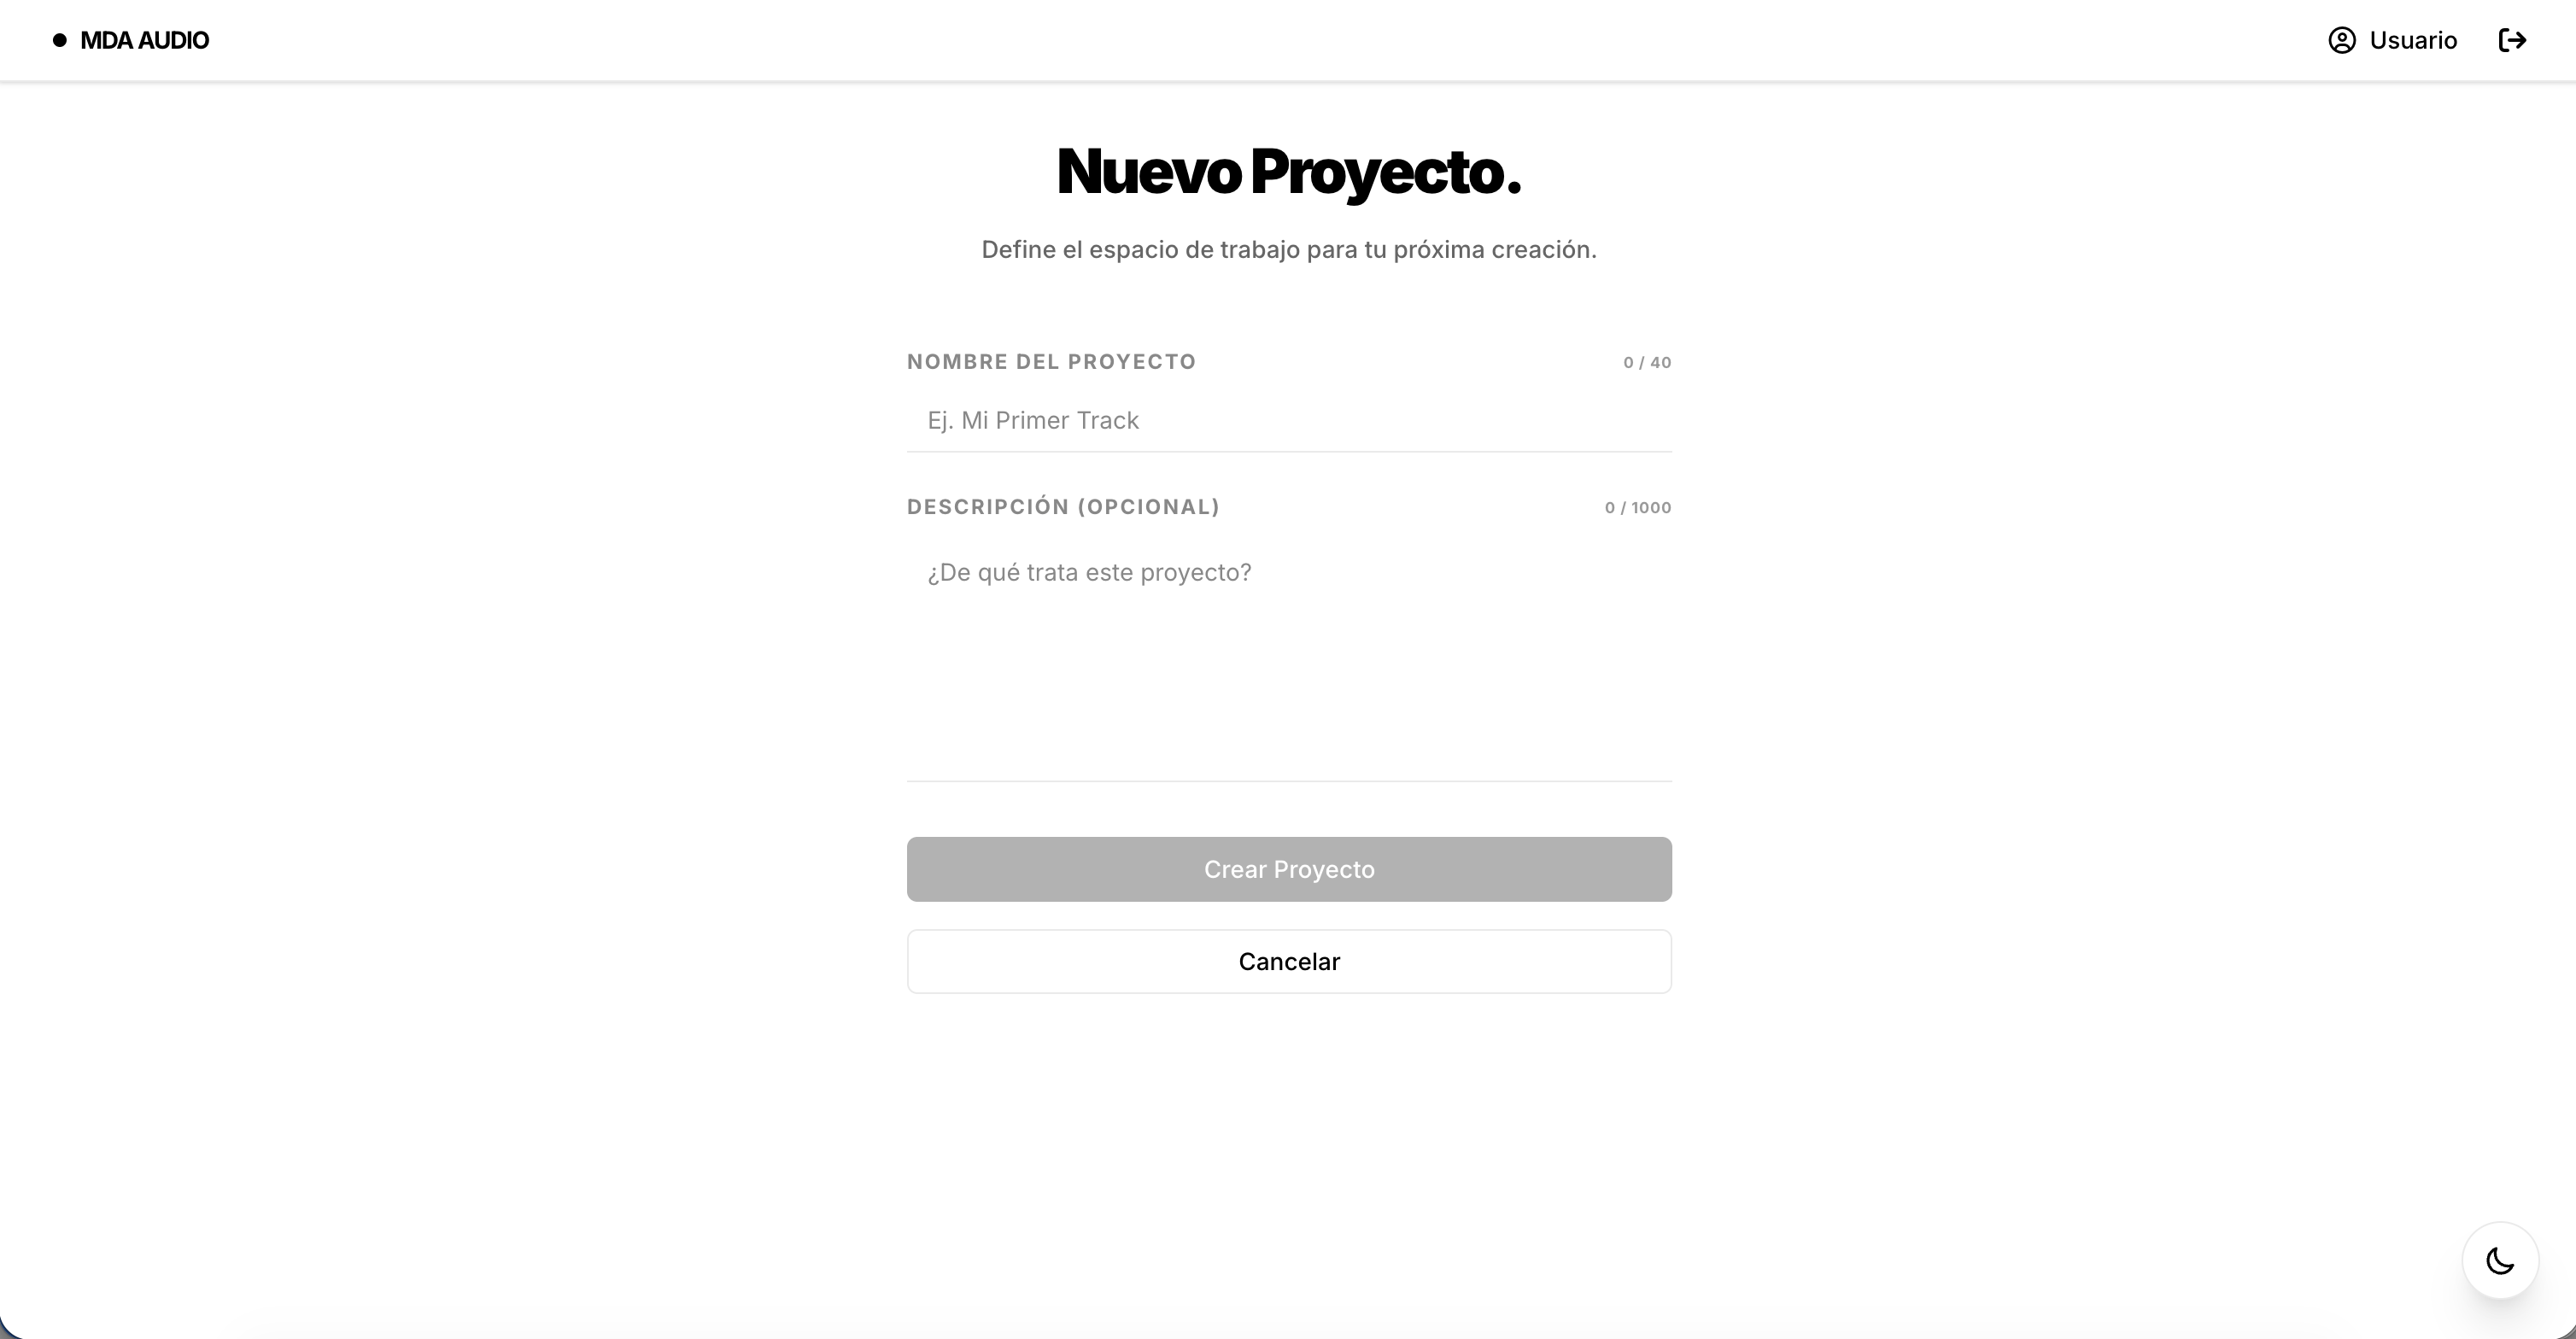
\includegraphics[width=0.6\textwidth]{imagenes/03_proyecto/02_AlPulsarNuevoProyecto.png}
    \caption{Formulario inicial al pulsar nuevo proyecto.}
\end{figure}

Al accionar la opción de crear un nuevo proyecto, se despliega un formulario. Este paso es fundamental, ya que define los metadatos básicos que identificarán al proyecto en el entorno.

\begin{figure}[!ht]
    \centering
    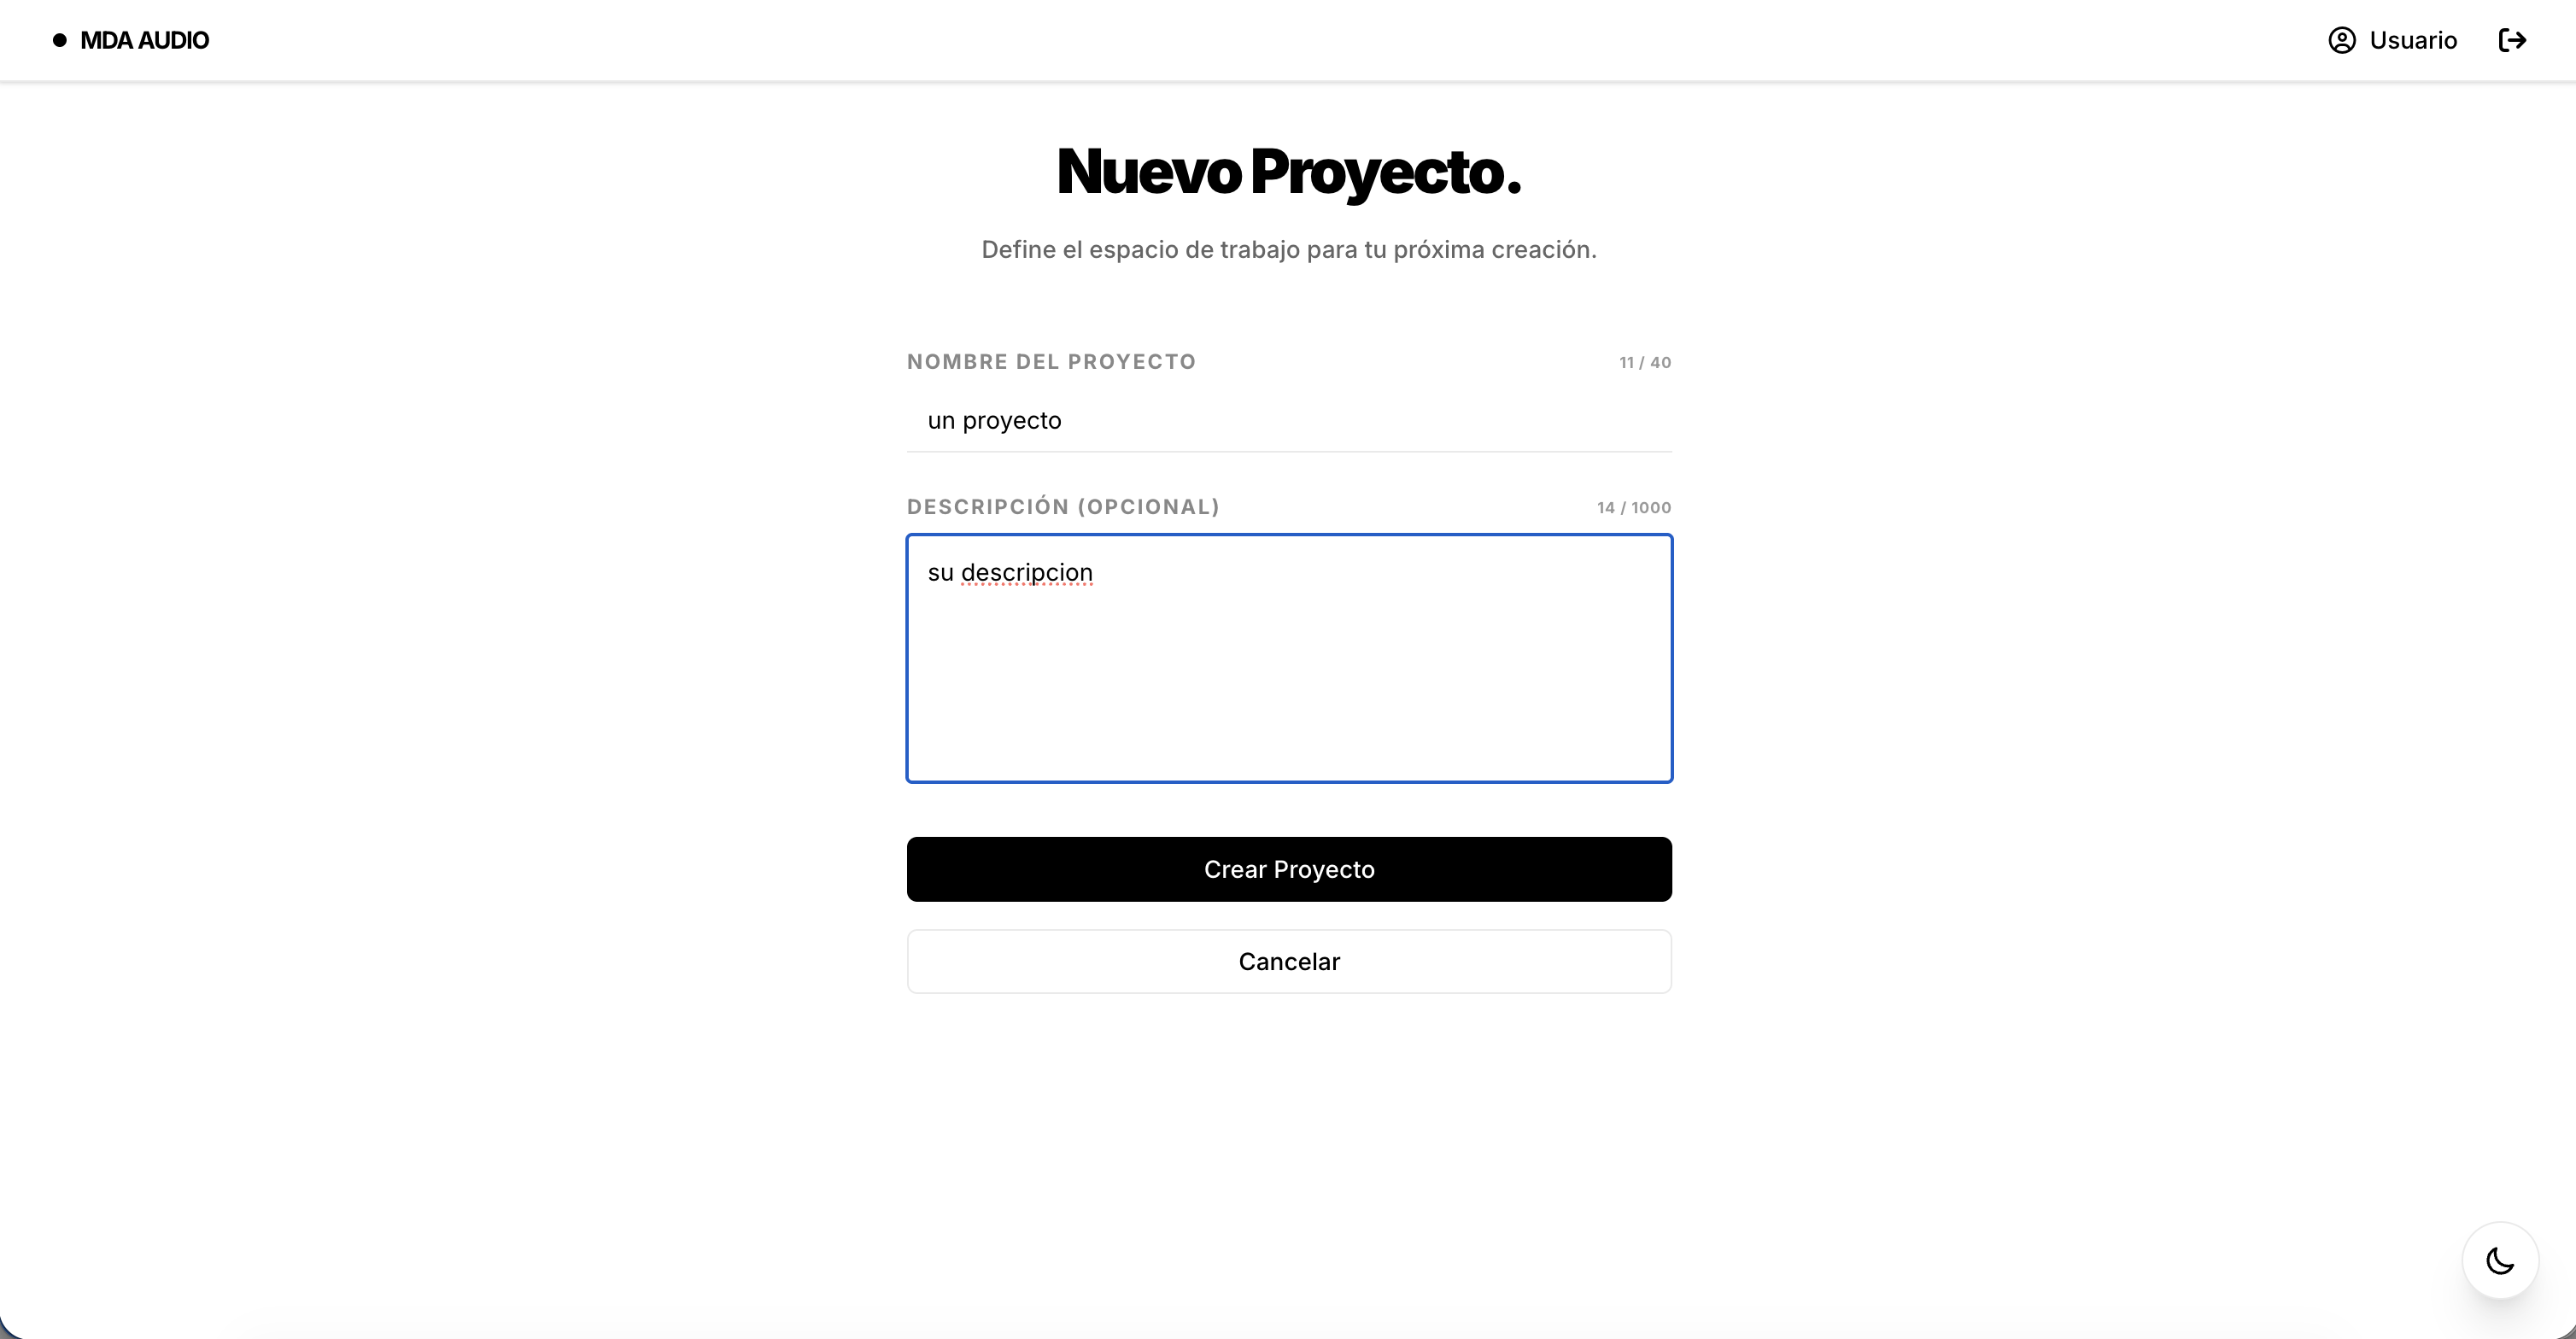
\includegraphics[width=0.6\textwidth]{imagenes/03_proyecto/03_rellenarInformacionNuevoProyecto.png}
    \caption{Relleno de información básica del nuevo proyecto.}
\end{figure}

El usuario debe completar la siguiente información:
\begin{itemize}
    \item \textbf{Nombre del proyecto:} Título descriptivo (ej. \textit{Sintetizador FM Avanzado}).
    \item \textbf{Descripción:} Detalle opcional sobre la finalidad del proyecto.
    \item \textbf{Color identificativo:} Selección de un color para la tarjeta del proyecto, facilitando su reconocimiento visual.
\end{itemize}

\begin{figure}[!ht]
    \centering
    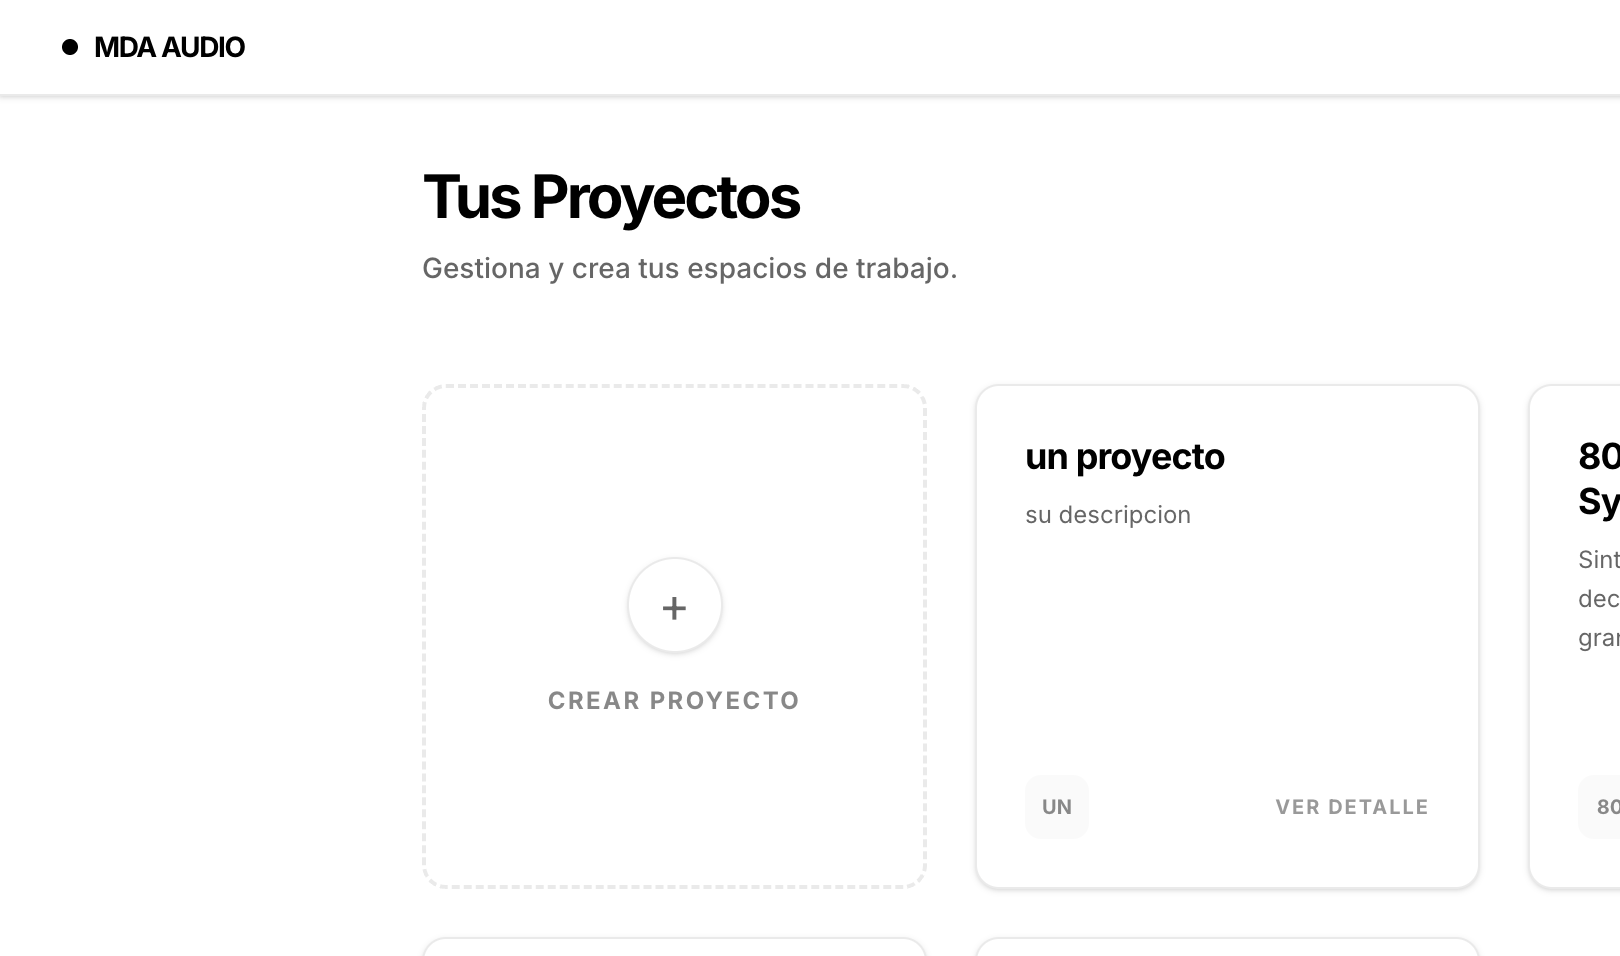
\includegraphics[width=0.6\textwidth]{imagenes/03_proyecto/04_nuevoProyectoCreado.png}
    \caption{Confirmación visual de la creación del proyecto.}
\end{figure}

Tras guardar los cambios, la aplicación confirma la creación y el proyecto aparece inmediatamente en el panel principal como una nueva tarjeta.

\subsection{Modificación y Eliminación}

Las tarjetas de los proyectos en el panel principal ofrecen opciones de gestión rápida sin necesidad de entrar a la edición profunda de modelos.

\begin{figure}[!ht]
    \centering
    
\includegraphics[width=0.4\textwidth]{imagenes/03_proyecto/05_botoneraModificacionYEliminacionProyecto.png}
    \caption{Botonera de opciones en la tarjeta de un proyecto.}
\end{figure}

Cada tarjeta incluye iconos contextuales que despliegan acciones de mantenimiento:
\begin{itemize}
    \item \textbf{Modificar:} Permite editar los metadatos (nombre, descripción, color).
    \item \textbf{Eliminar:} Permite borrar el proyecto y todo su contenido asociado de forma permanente.
\end{itemize}

\begin{figure}[!ht]
    \centering
    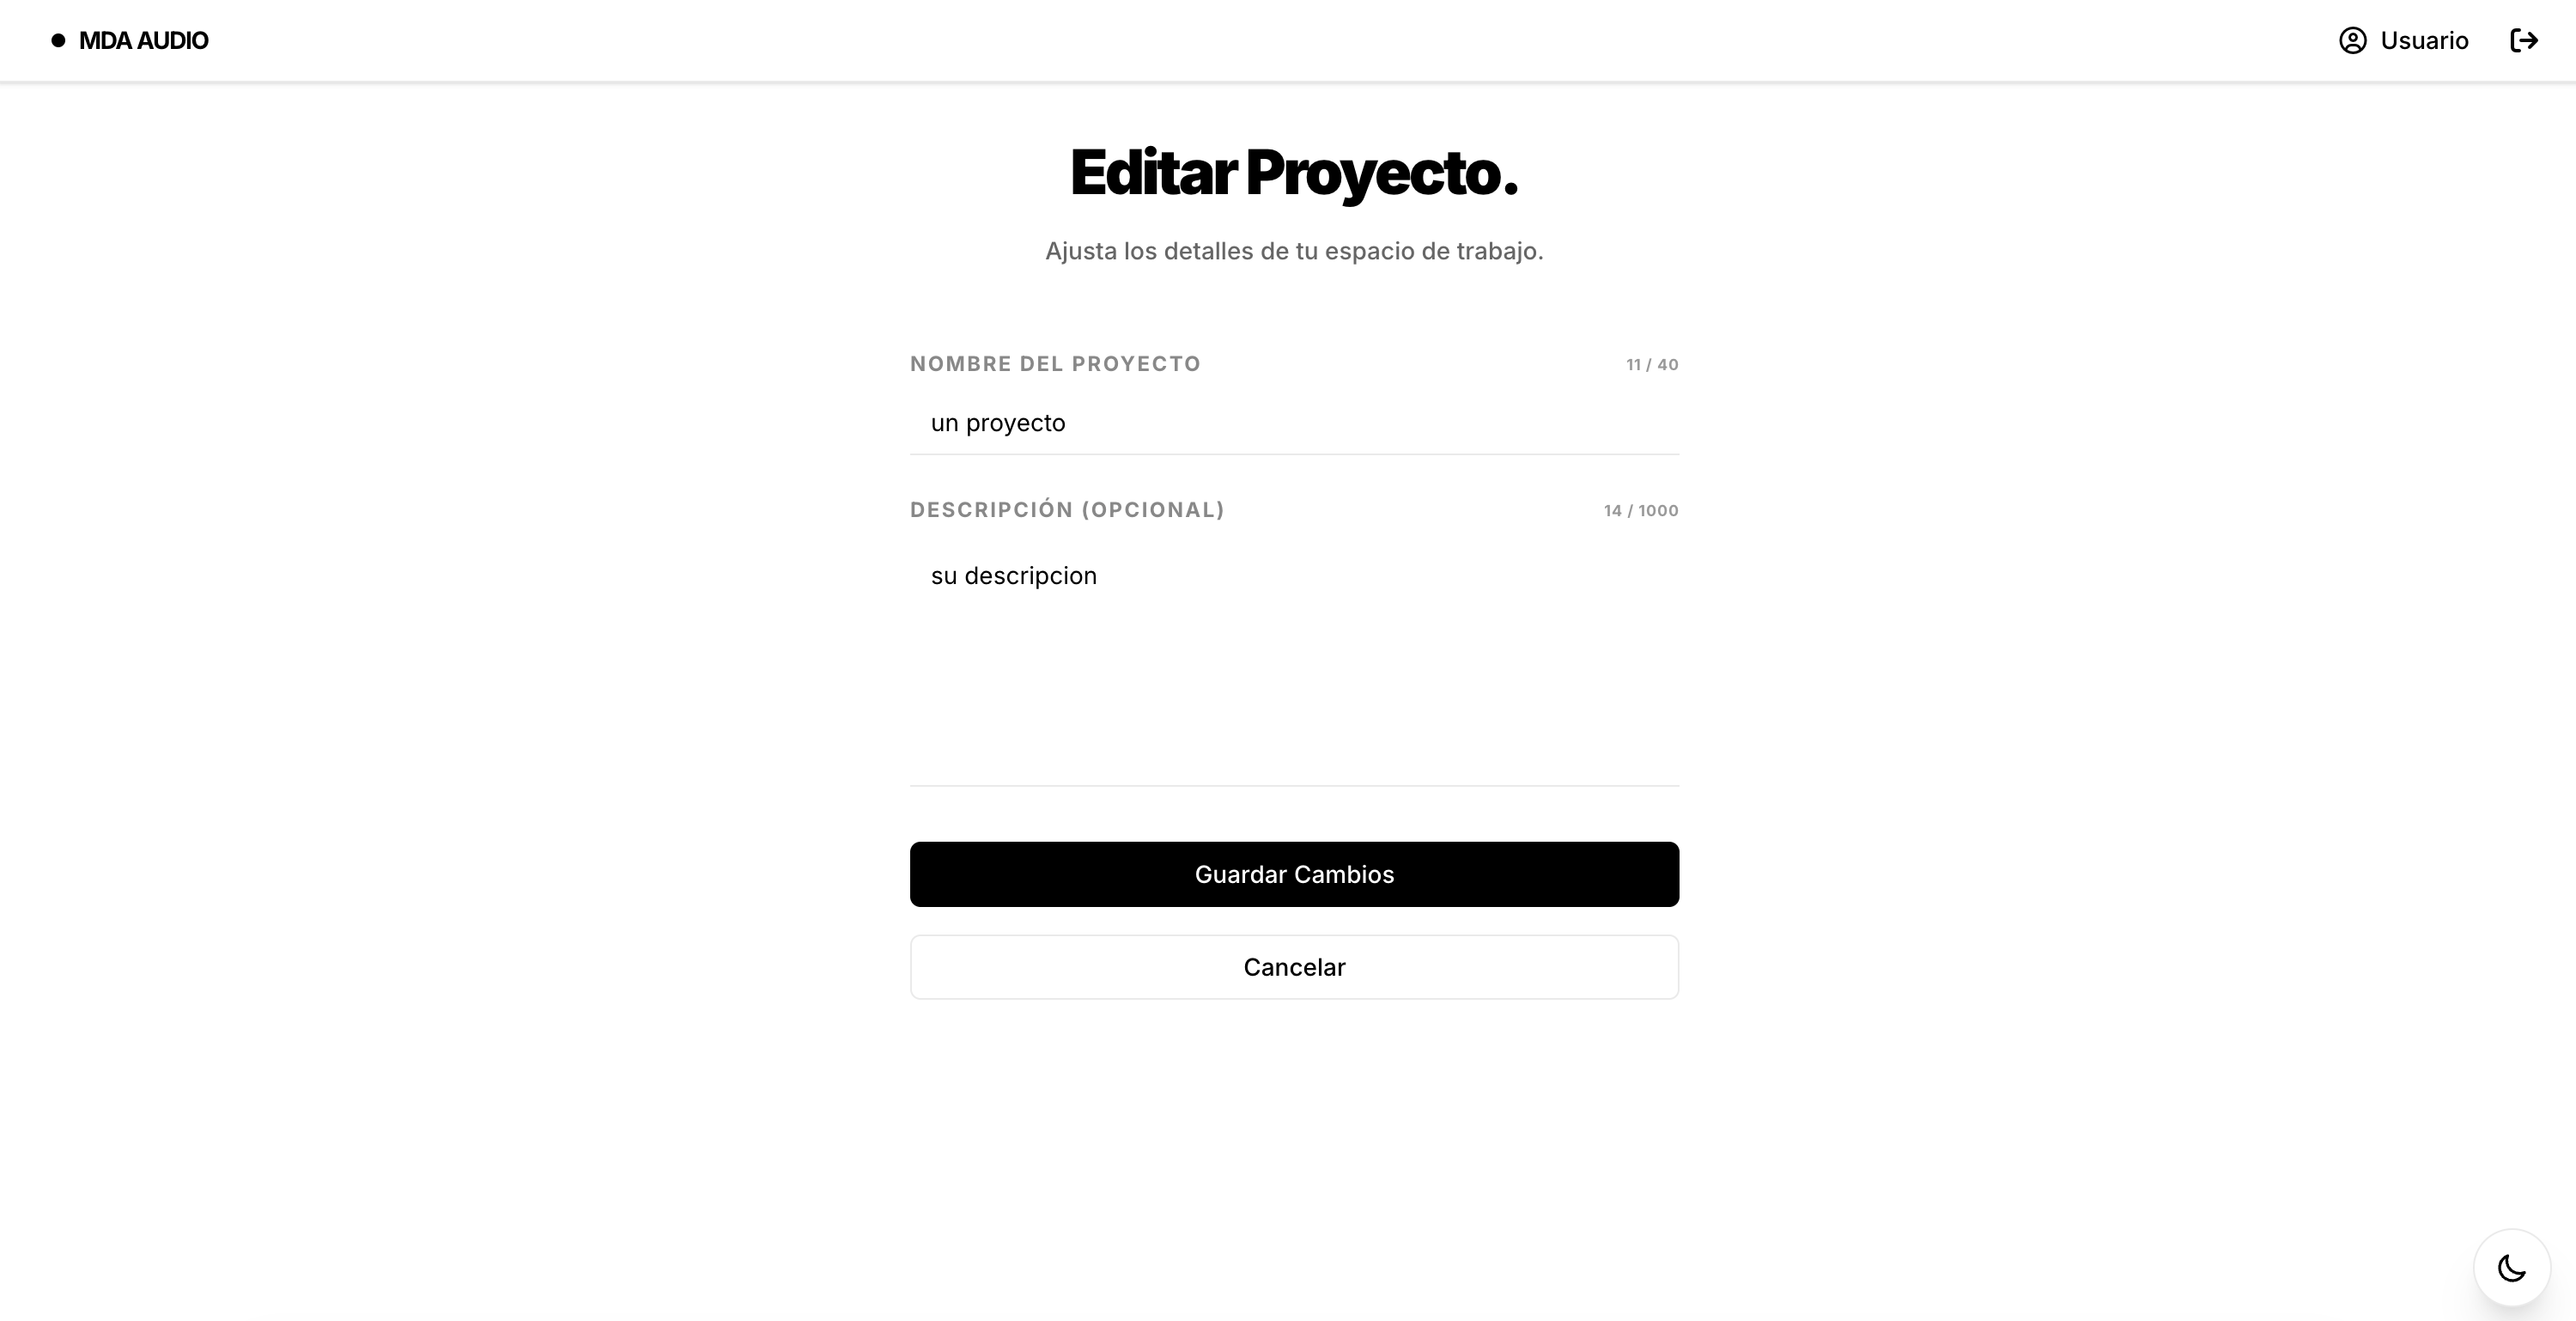
\includegraphics[width=0.6\textwidth]{imagenes/03_proyecto/06_pulsadoBotonModificarProyecto.png}
    \caption{Formulario al pulsar el botón de modificar proyecto.}
\end{figure}

Al seleccionar modificar, se abre el mismo formulario de creación, pero con los datos actuales cargados, permitiendo actualizarlos fácilmente.

\begin{figure}[!ht]
    \centering
    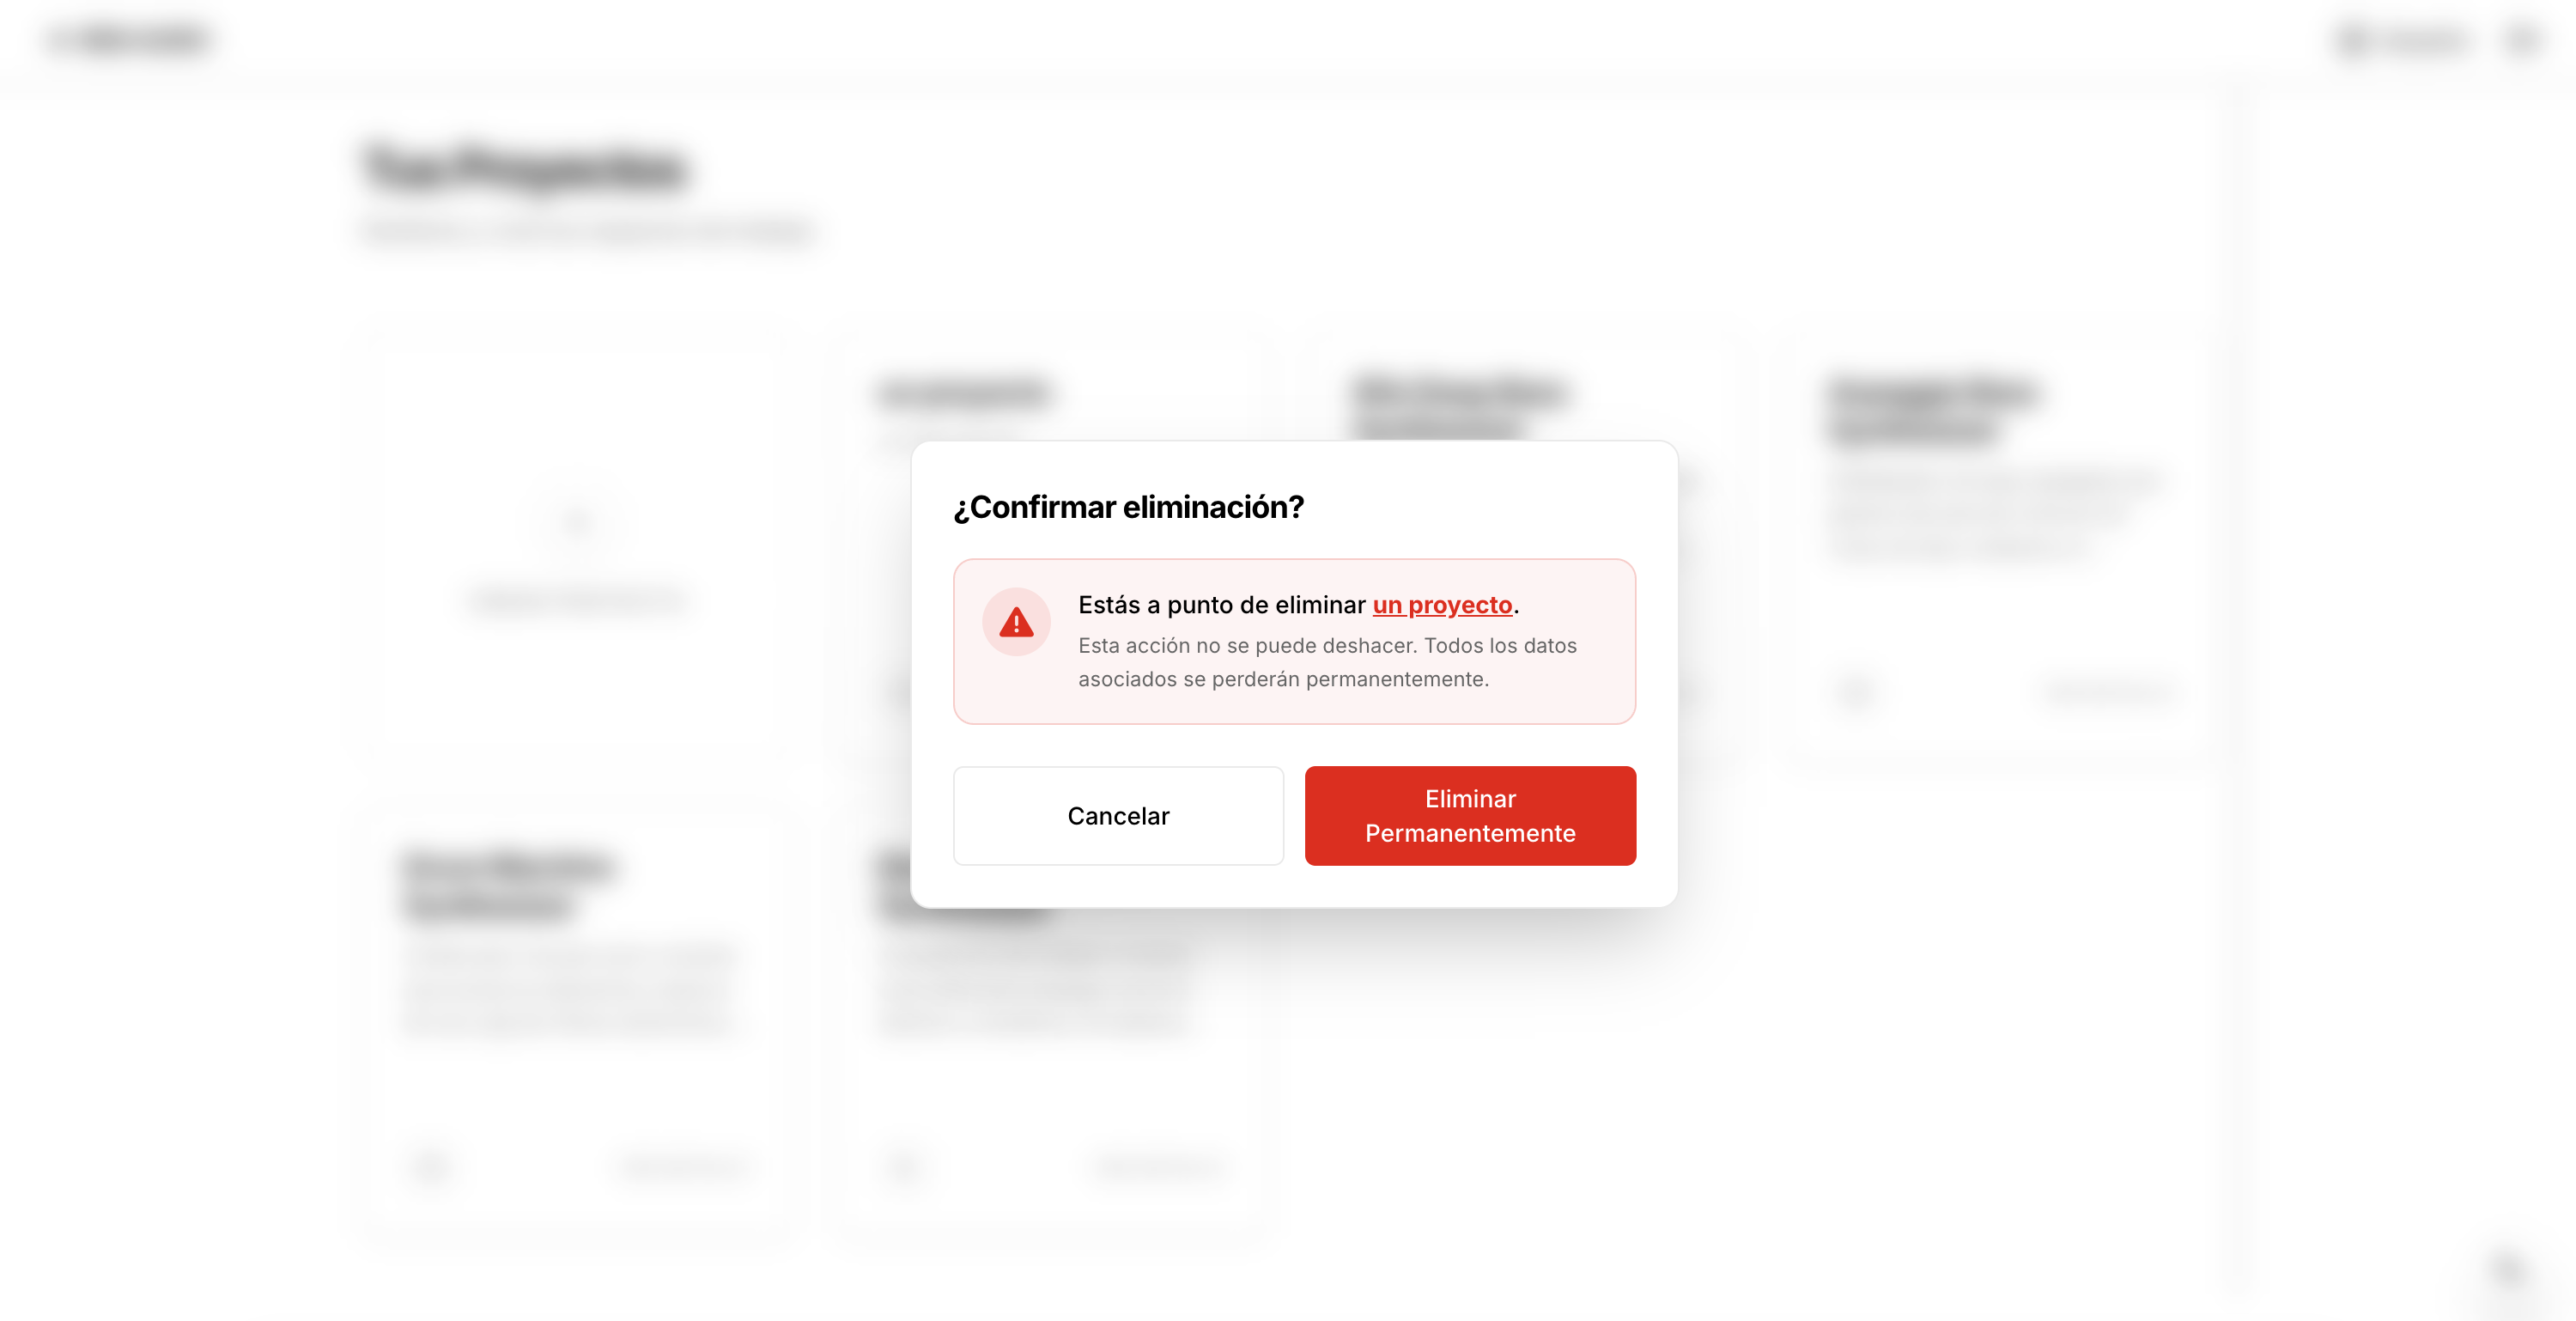
\includegraphics[width=0.6\textwidth]{imagenes/03_proyecto/07_pulsadoBotonEliminarProyecto.png}
    \caption{Aviso de confirmación al eliminar un proyecto.}
\end{figure}

La opción de eliminar es destructiva. Por ello, el sistema siempre solicita una confirmación explícita para evitar pérdidas de trabajo accidentales. Una vez confirmado, el proyecto y sus definiciones en lenguajes \textit{DSL} son eliminados irreversiblemente.

\subsection{Acceso al Espacio de Trabajo del Proyecto}

Para empezar a modelar y definir la lógica musical y el diseño conceptual, el usuario debe abrir el proyecto.

\begin{figure}[!ht]
    \centering
    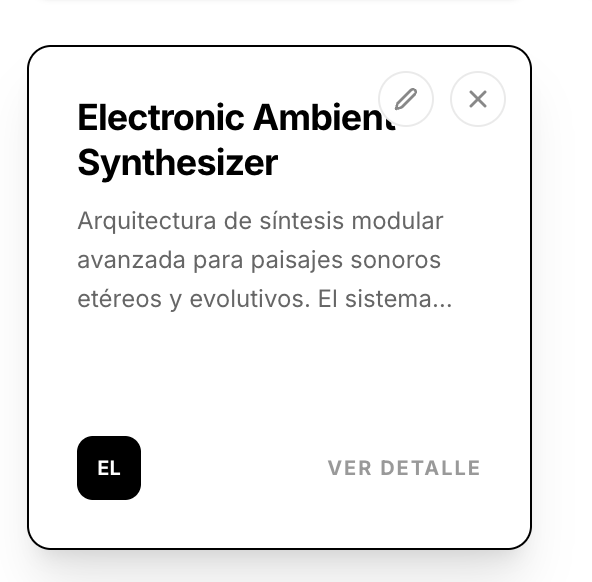
\includegraphics[width=0.6\textwidth]{imagenes/03_proyecto/08_vistaContenidoCajaDeUnProyectoParaPulsarYAbrir.png}
    \caption{Área clicable de la tarjeta para abrir el proyecto.}
\end{figure}

Haciendo clic sobre cualquier parte del contenido de la tarjeta del proyecto (fuera de los botones de modificar/eliminar), el sistema navega al espacio de trabajo específico de dicho proyecto.

\begin{figure}[!ht]
    \centering
    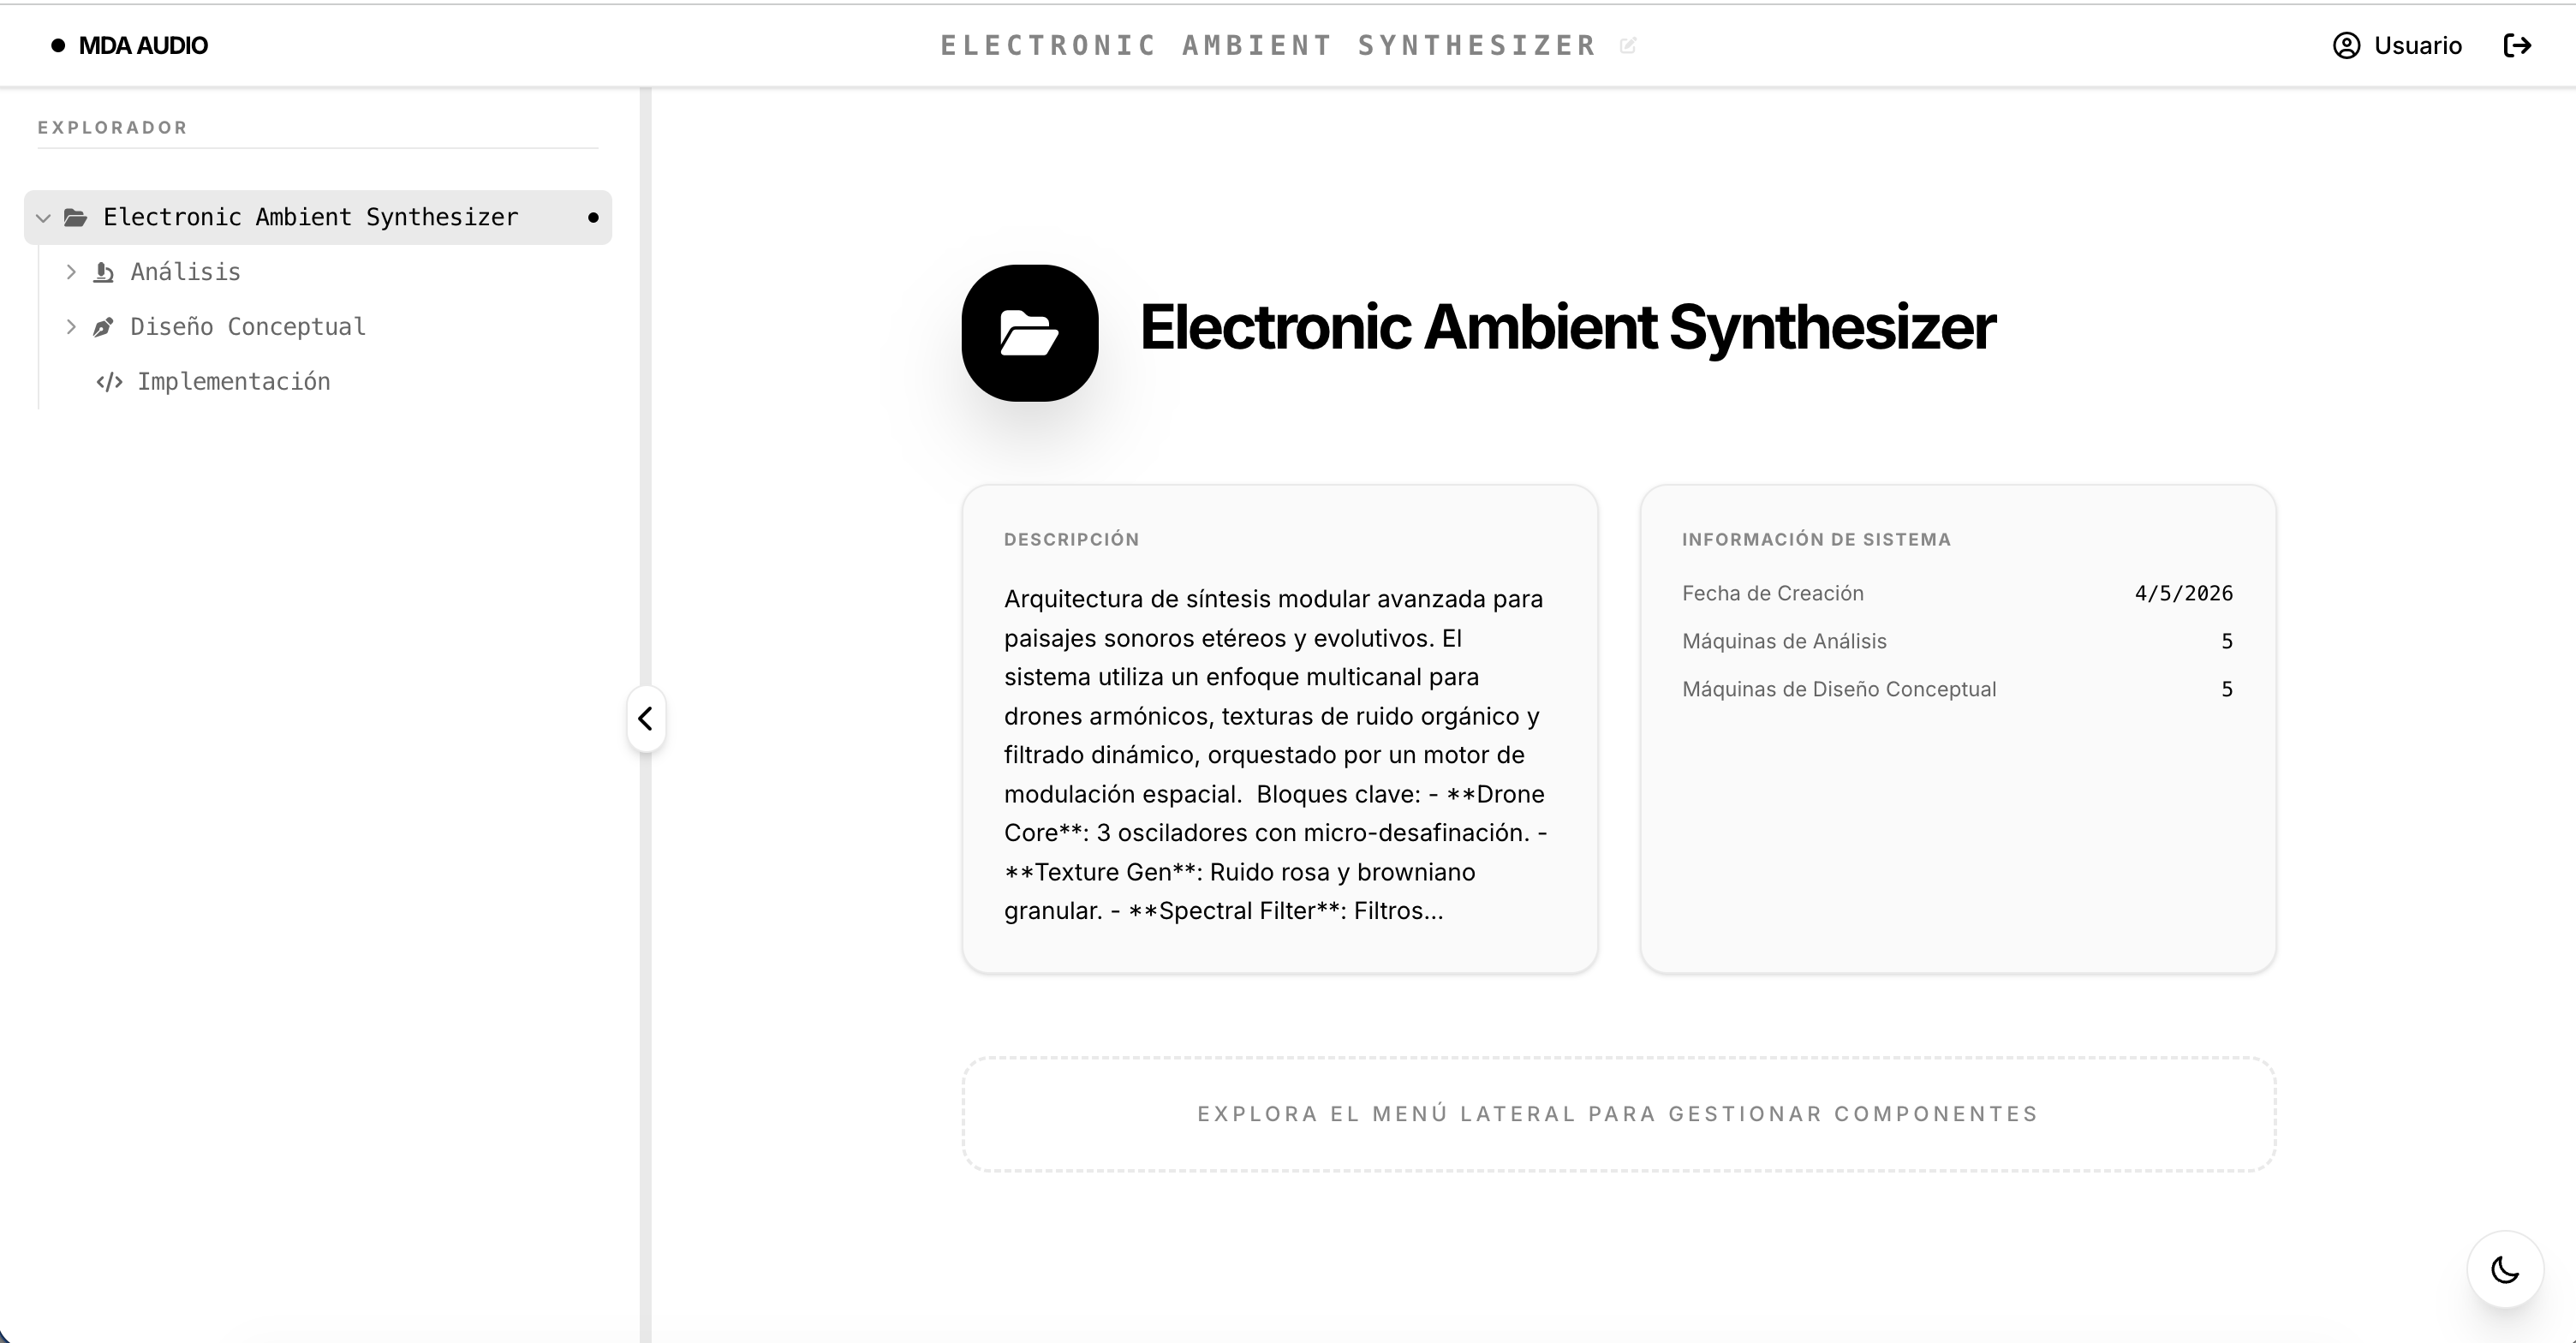
\includegraphics[width=\textwidth]{imagenes/03_proyecto/09_pantallaPrincipalDeProyectoAbierto.png}
    \caption{Pantalla principal tras abrir un proyecto.}
\end{figure}

Dentro de esta pantalla se encuentra el entorno central de la aplicación \textit{MDAA}. Desde aquí se gestionan los modelos independientes de computación (\textit{CIM}) y de plataforma (\textit{PIM}). El proyecto abierto permite también modificar su información básica desde esta misma vista.

\begin{figure}[!ht]
    \centering
    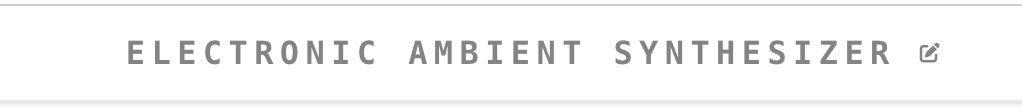
\includegraphics[width=0.4\textwidth]{imagenes/03_proyecto/10_botonModificarInfoBasicaProyectoDentroPantallaProyecto.png}
    \caption{Botón para modificar información básica dentro del proyecto.}
\end{figure}

\begin{figure}[!ht]
    \centering
    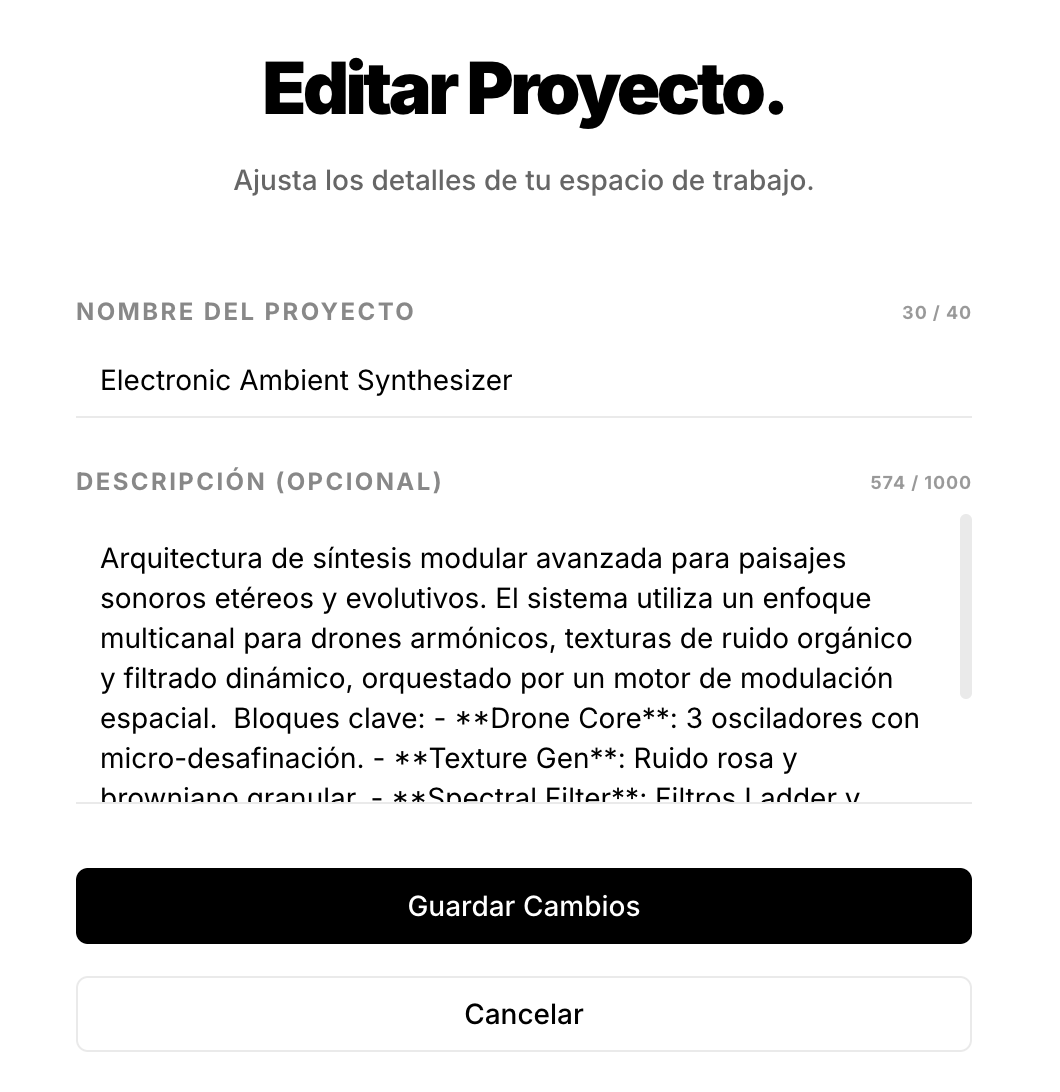
\includegraphics[width=0.6\textwidth]{imagenes/03_proyecto/11_pantallaModificarInfoBasicaProyecto.png}
    \caption{Pantalla de modificación de información básica desde el interior del proyecto.}
\end{figure}

Este botón despliega nuevamente el formulario de metadatos, garantizando que el usuario pueda ajustar el nombre o descripción sin necesidad de regresar al panel principal.

\section{Gestión de Cuenta y Sesión}

Desde el panel principal y cualquier otra vista global, la aplicación ofrece controles de sesión de usuario en la esquina superior derecha.

\begin{figure}[!ht]
    \centering
    
\includegraphics[width=0.4\textwidth]{imagenes/03_proyecto/12_botoneraGestionUsuarioDentroPantallaPrincipal.png}
    \caption{Botonera de gestión de usuario en la barra de navegación superior.}
\end{figure}

\begin{figure}[H]
    \centering
    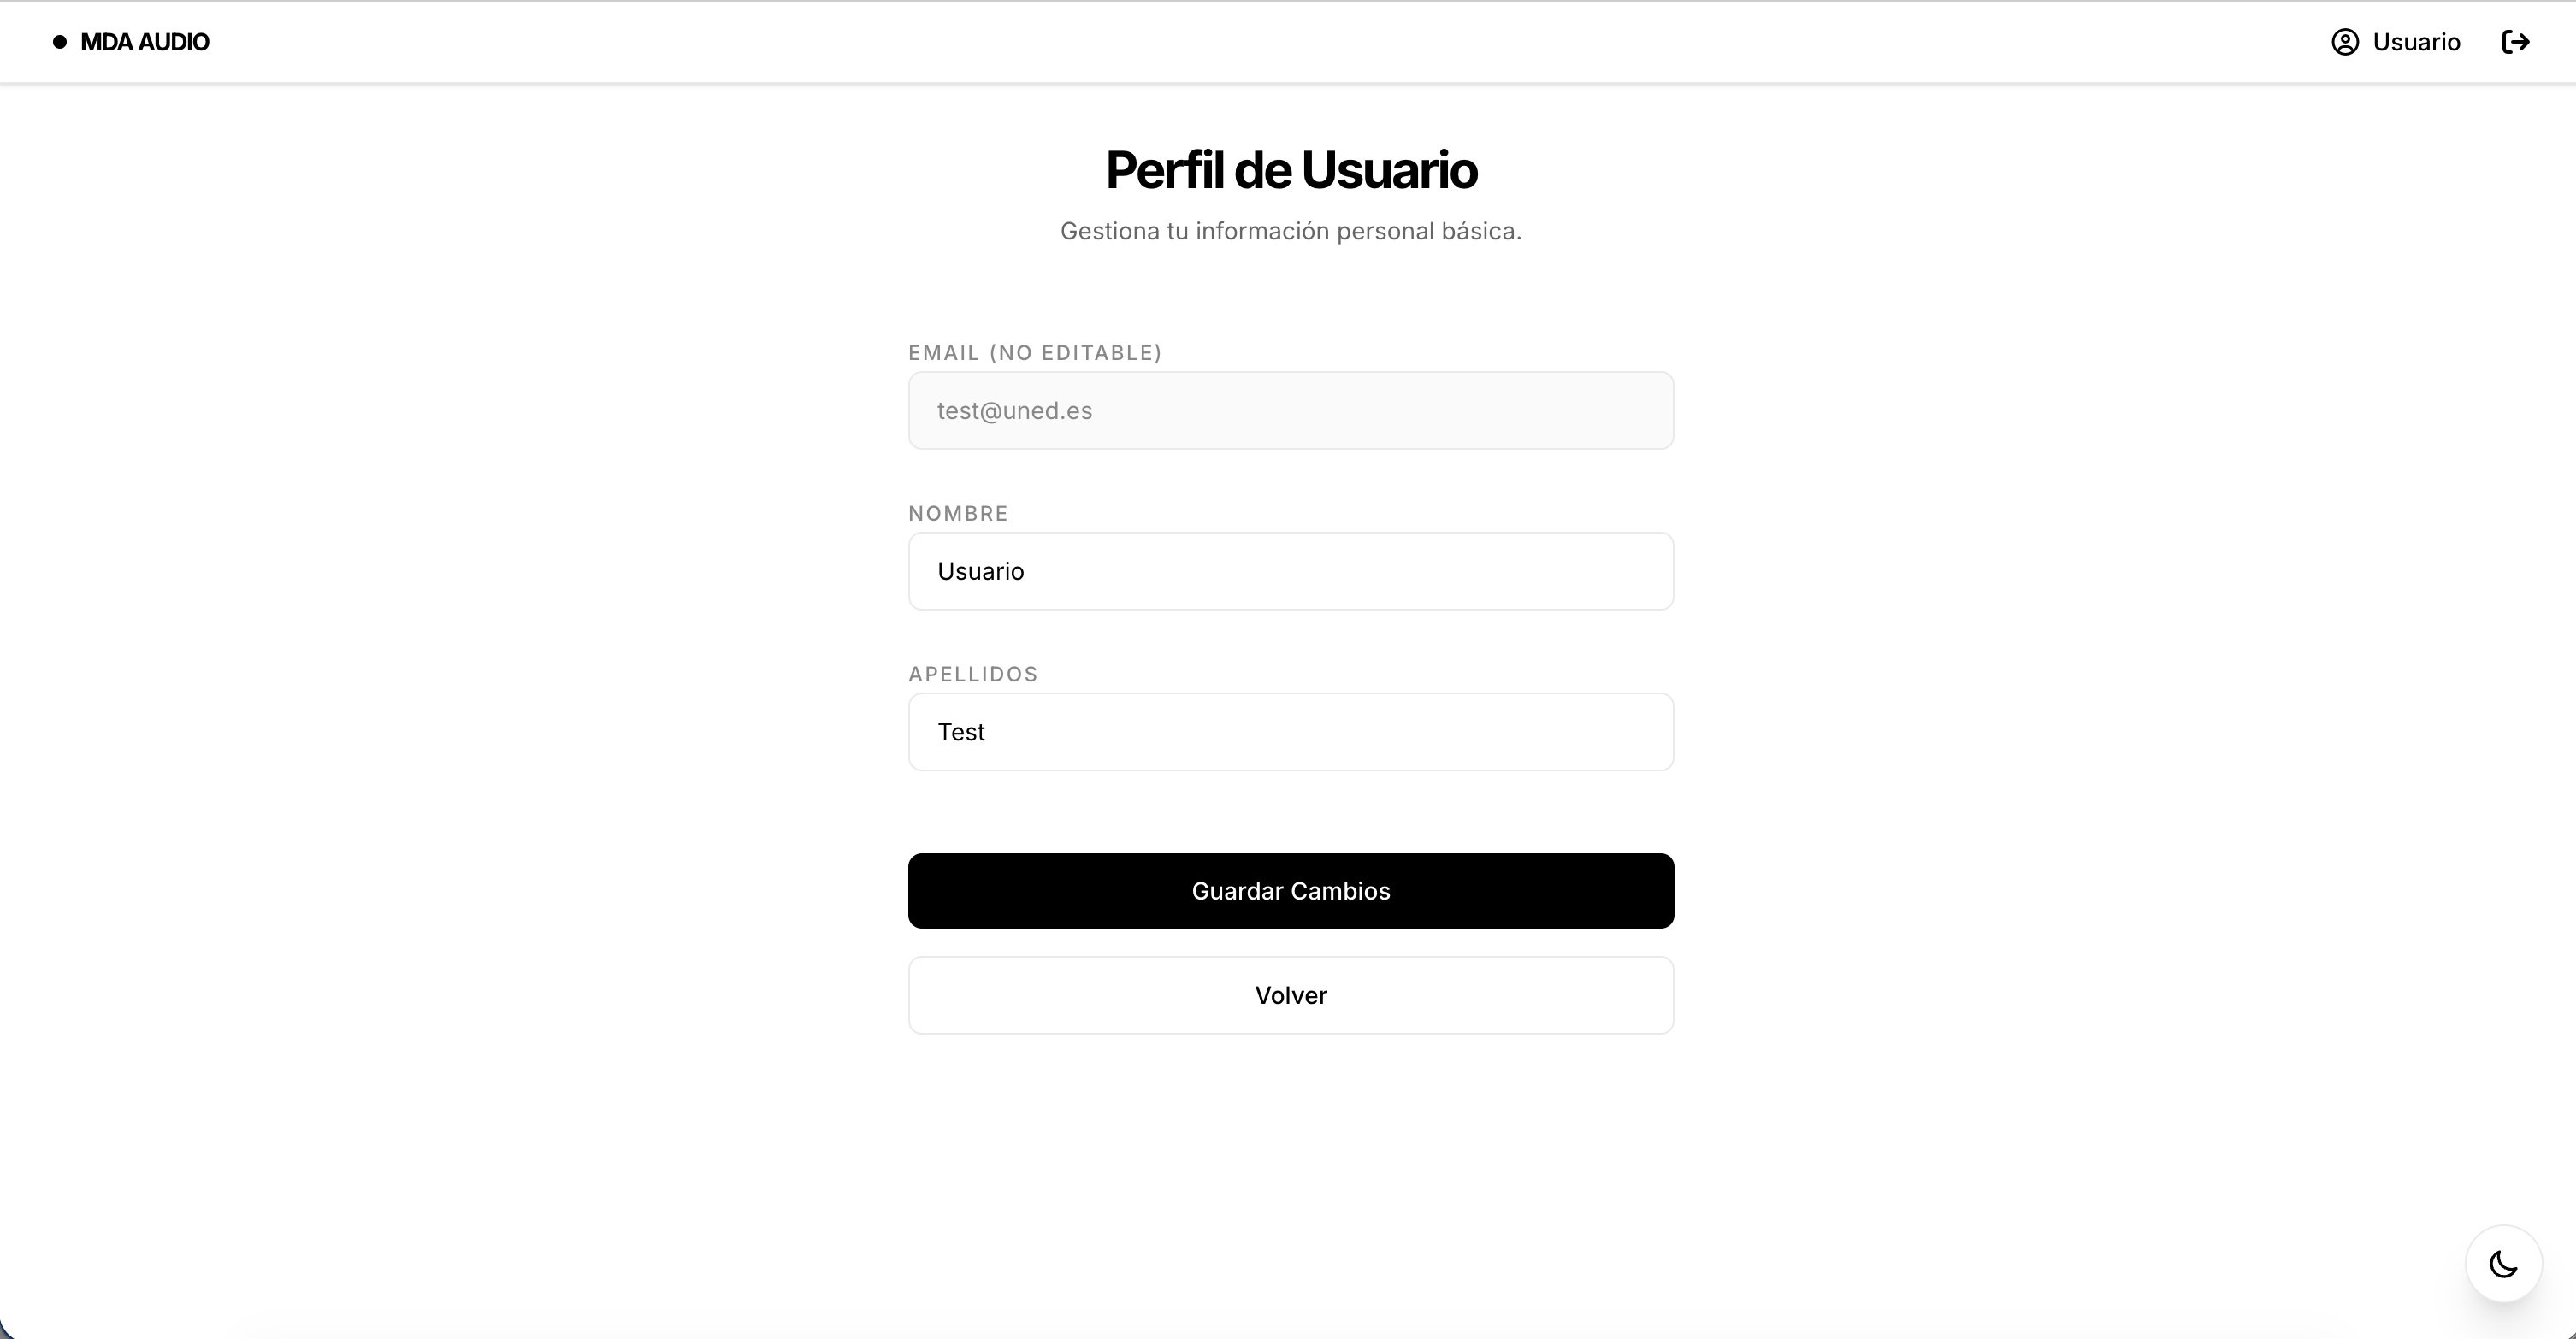
\includegraphics[width=0.5\textwidth]{imagenes/03_proyecto/14_botonUsuarioPulsadoDeGestionUsuarioEnPantallaPrincipal.png}
    \caption{Menú desplegable del usuario.}
\end{figure}

Al pulsar sobre el nombre o icono del usuario, se despliega un menú que incluye:
\begin{itemize}
    \item \textbf{Cerrar Sesión:} Permite salir de forma segura de la aplicación.
\end{itemize}

\begin{figure}[H]
    \centering
    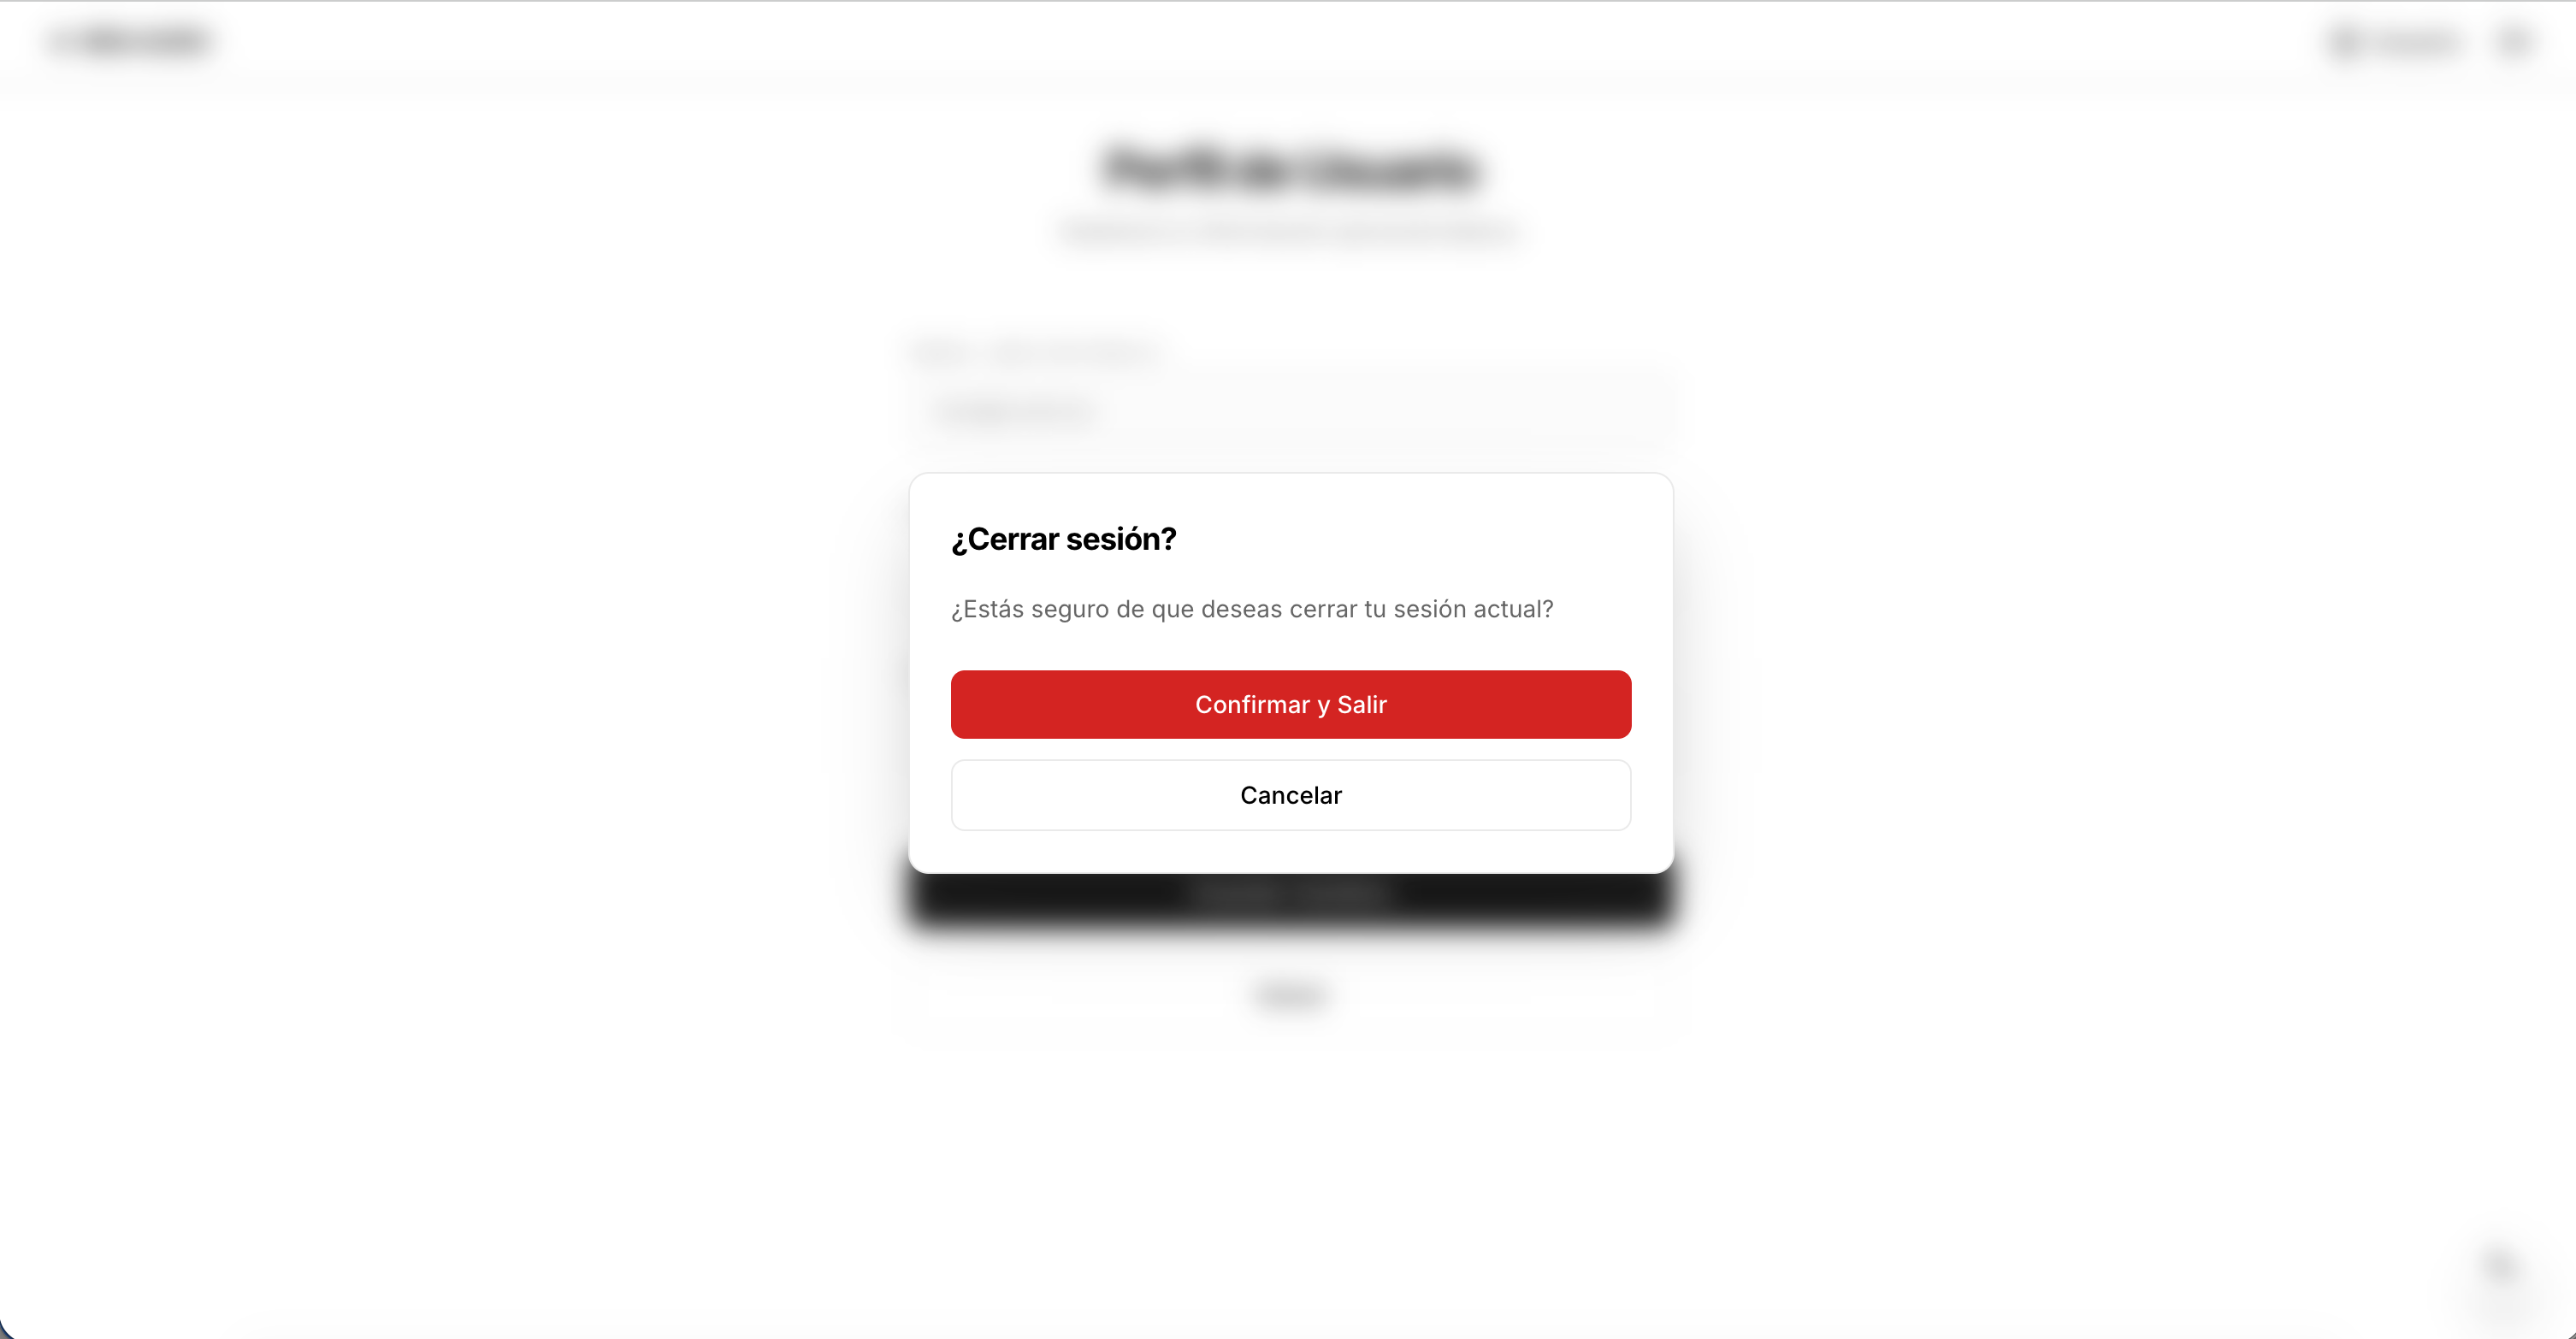
\includegraphics[width=0.6\textwidth]{imagenes/03_proyecto/13_botonCerrarSesionPulsado.png}
    \caption{Aviso de confirmación para cerrar sesión.}
\end{figure}

El sistema solicita confirmación antes de cerrar la sesión, redirigiendo posteriormente a la pantalla de inicio principal.

\begin{figure}[H]
    \centering
    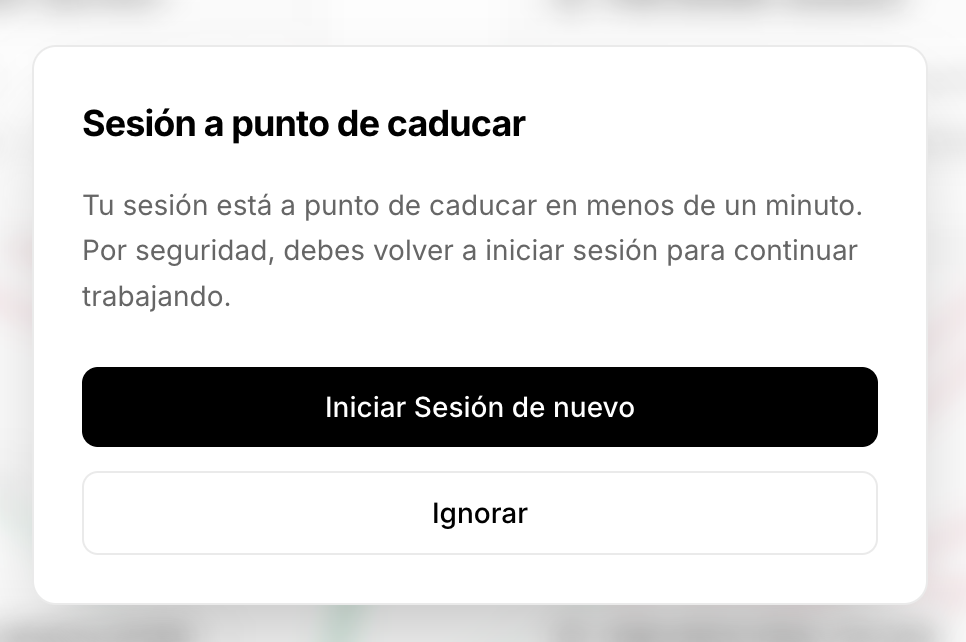
\includegraphics[width=0.6\textwidth]{imagenes/03_proyecto/15_sesionAPuntoDeCaducar.png}
    \caption{Aviso de seguridad por sesión próxima a caducar.}
\end{figure}

Por motivos de seguridad, la sesión tiene un tiempo de expiración. Cuando la sesión está a punto de caducar por inactividad, la aplicación muestra una advertencia, permitiendo al usuario extenderla o dejar que expire, tras lo cual deberá volver a introducir sus credenciales.

\chapter{Estructura del Espacio de Trabajo}

\section{Disposición General}

El núcleo de la aplicación \textit{MDAA} reside en el espacio de trabajo que se habilita al abrir un proyecto. Esta vista está diseñada para maximizar la eficiencia y organizar lógicamente todas las herramientas necesarias para la definición de sintetizadores musicales.



\begin{figure}[!ht]
    \centering
    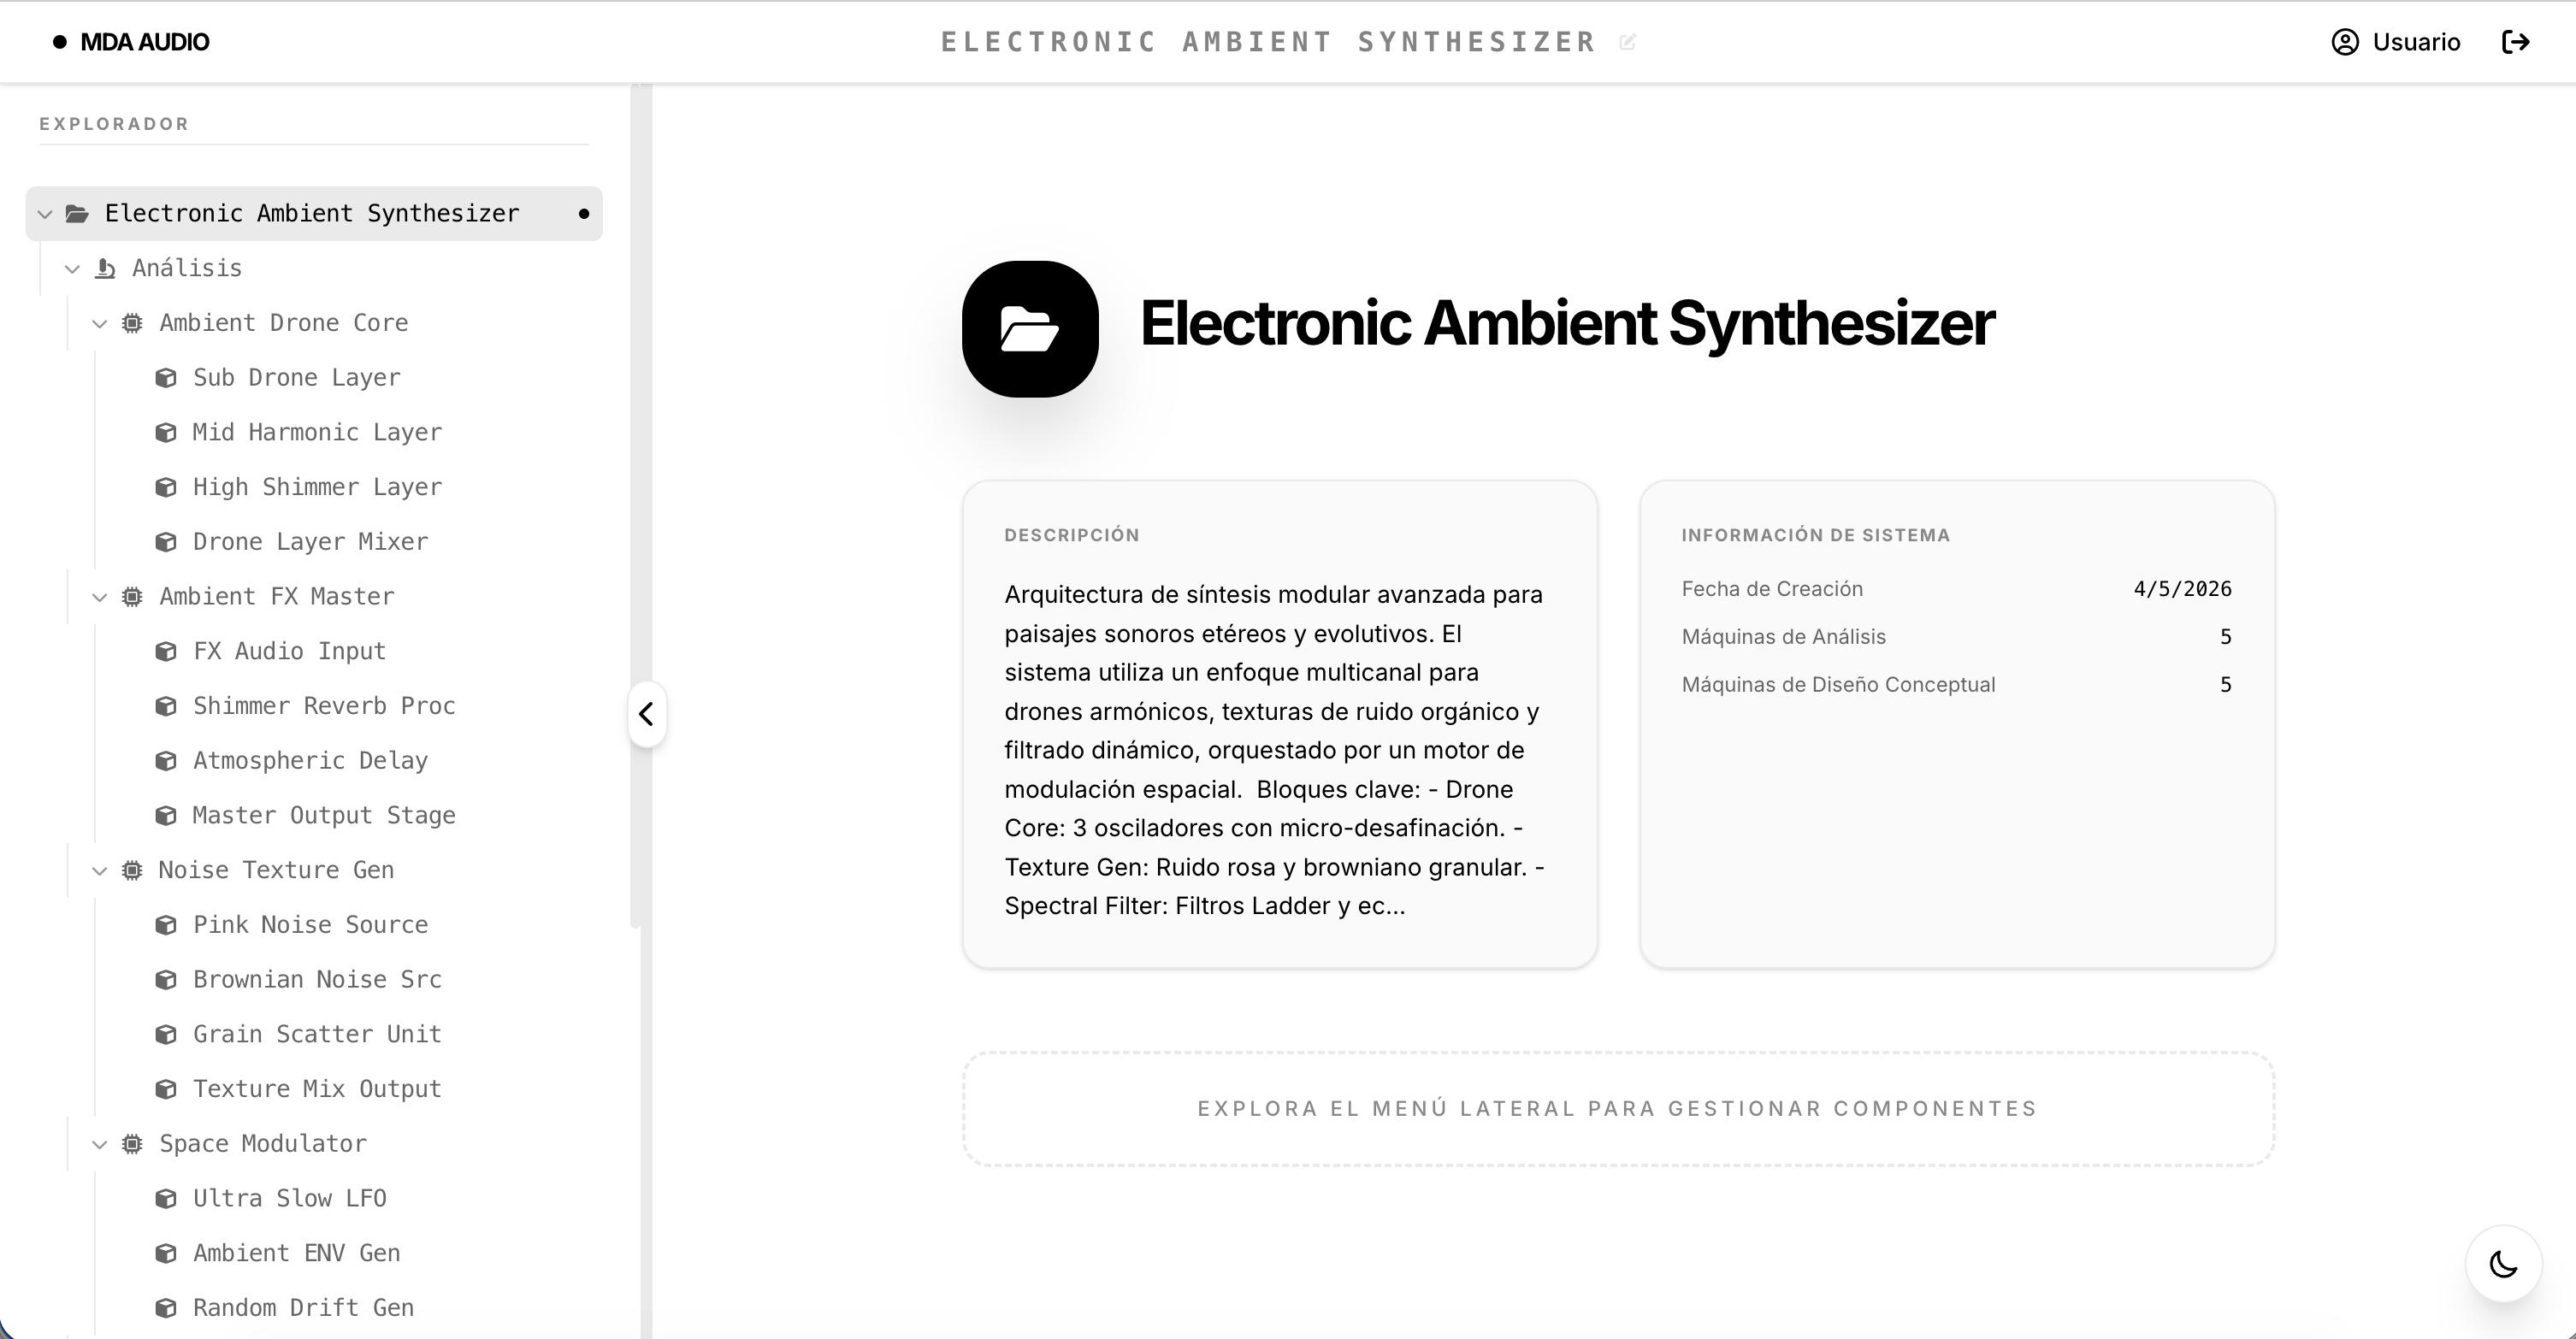
\includegraphics[width=\textwidth]{imagenes/04_estructura/01_pantallaPrincipalProyectoConSus3Partes.png}
    \caption{Pantalla principal del proyecto dividida en tres áreas fundamentales.}
\end{figure}

La interfaz del espacio de trabajo se divide estructuralmente en tres partes principales:
\begin{itemize}
    \item \textbf{Barra Principal Superior:} Contiene controles globales de navegación, gestión de la vista y acciones críticas del proyecto.
    \item \textbf{Explorador del Proyecto (Panel Izquierdo):} Muestra la estructura jerárquica de los elementos del proyecto, facilitando la navegación entre modelos de análisis y diseño.
    \item \textbf{Área de Trabajo Central:} Es el lienzo principal donde se abren los editores visuales y textuales para interactuar con los elementos del dominio.
\end{itemize}

\subsection{El Explorador del Proyecto}

El explorador es el panel lateral que organiza el contenido. Funciona como un árbol de directorios que clasifica los modelos según la metodología \textit{MDAA}.

\begin{figure}[!ht]
    \centering
    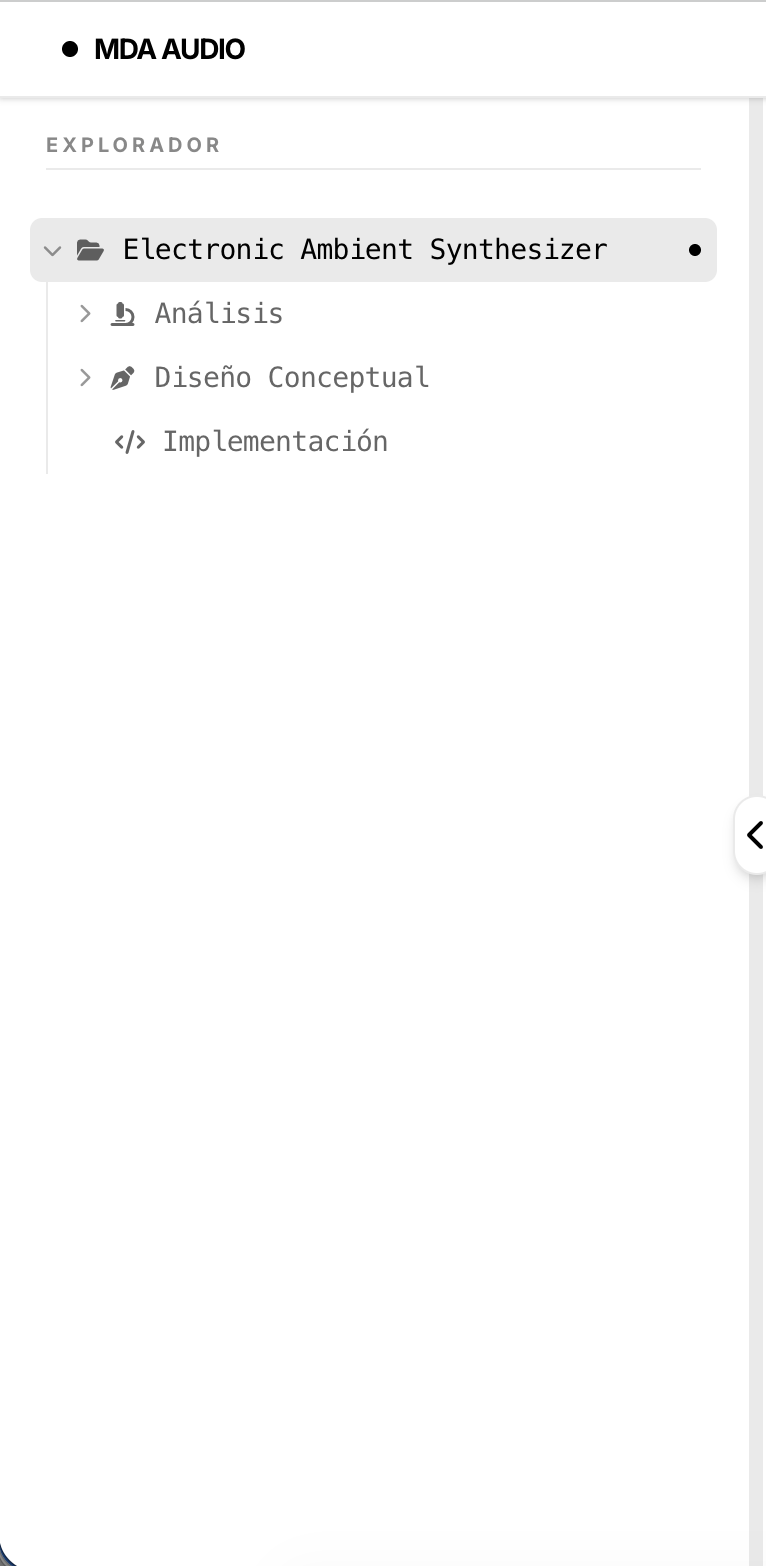
\includegraphics[width=0.4\textwidth]{imagenes/04_estructura/03_exploradorDelProyecto.png}
    \caption{Detalle del explorador jerárquico del proyecto.}
\end{figure}

En el explorador se distinguen claramente dos ramas principales:
\begin{itemize}
    \item \textbf{Análisis Conceptual (CIM):} Donde se definen los modelos independientes de la computación, capturando los requerimientos del dominio musical.
    \item \textbf{Diseño Conceptual (PIM):} Donde se establece la arquitectura independiente de plataforma, basándose en el análisis previo.
\end{itemize}
Al pulsar sobre cualquier elemento del árbol, este se abre como una pestaña en el área de trabajo central.

\begin{figure}[!ht]
    \centering
    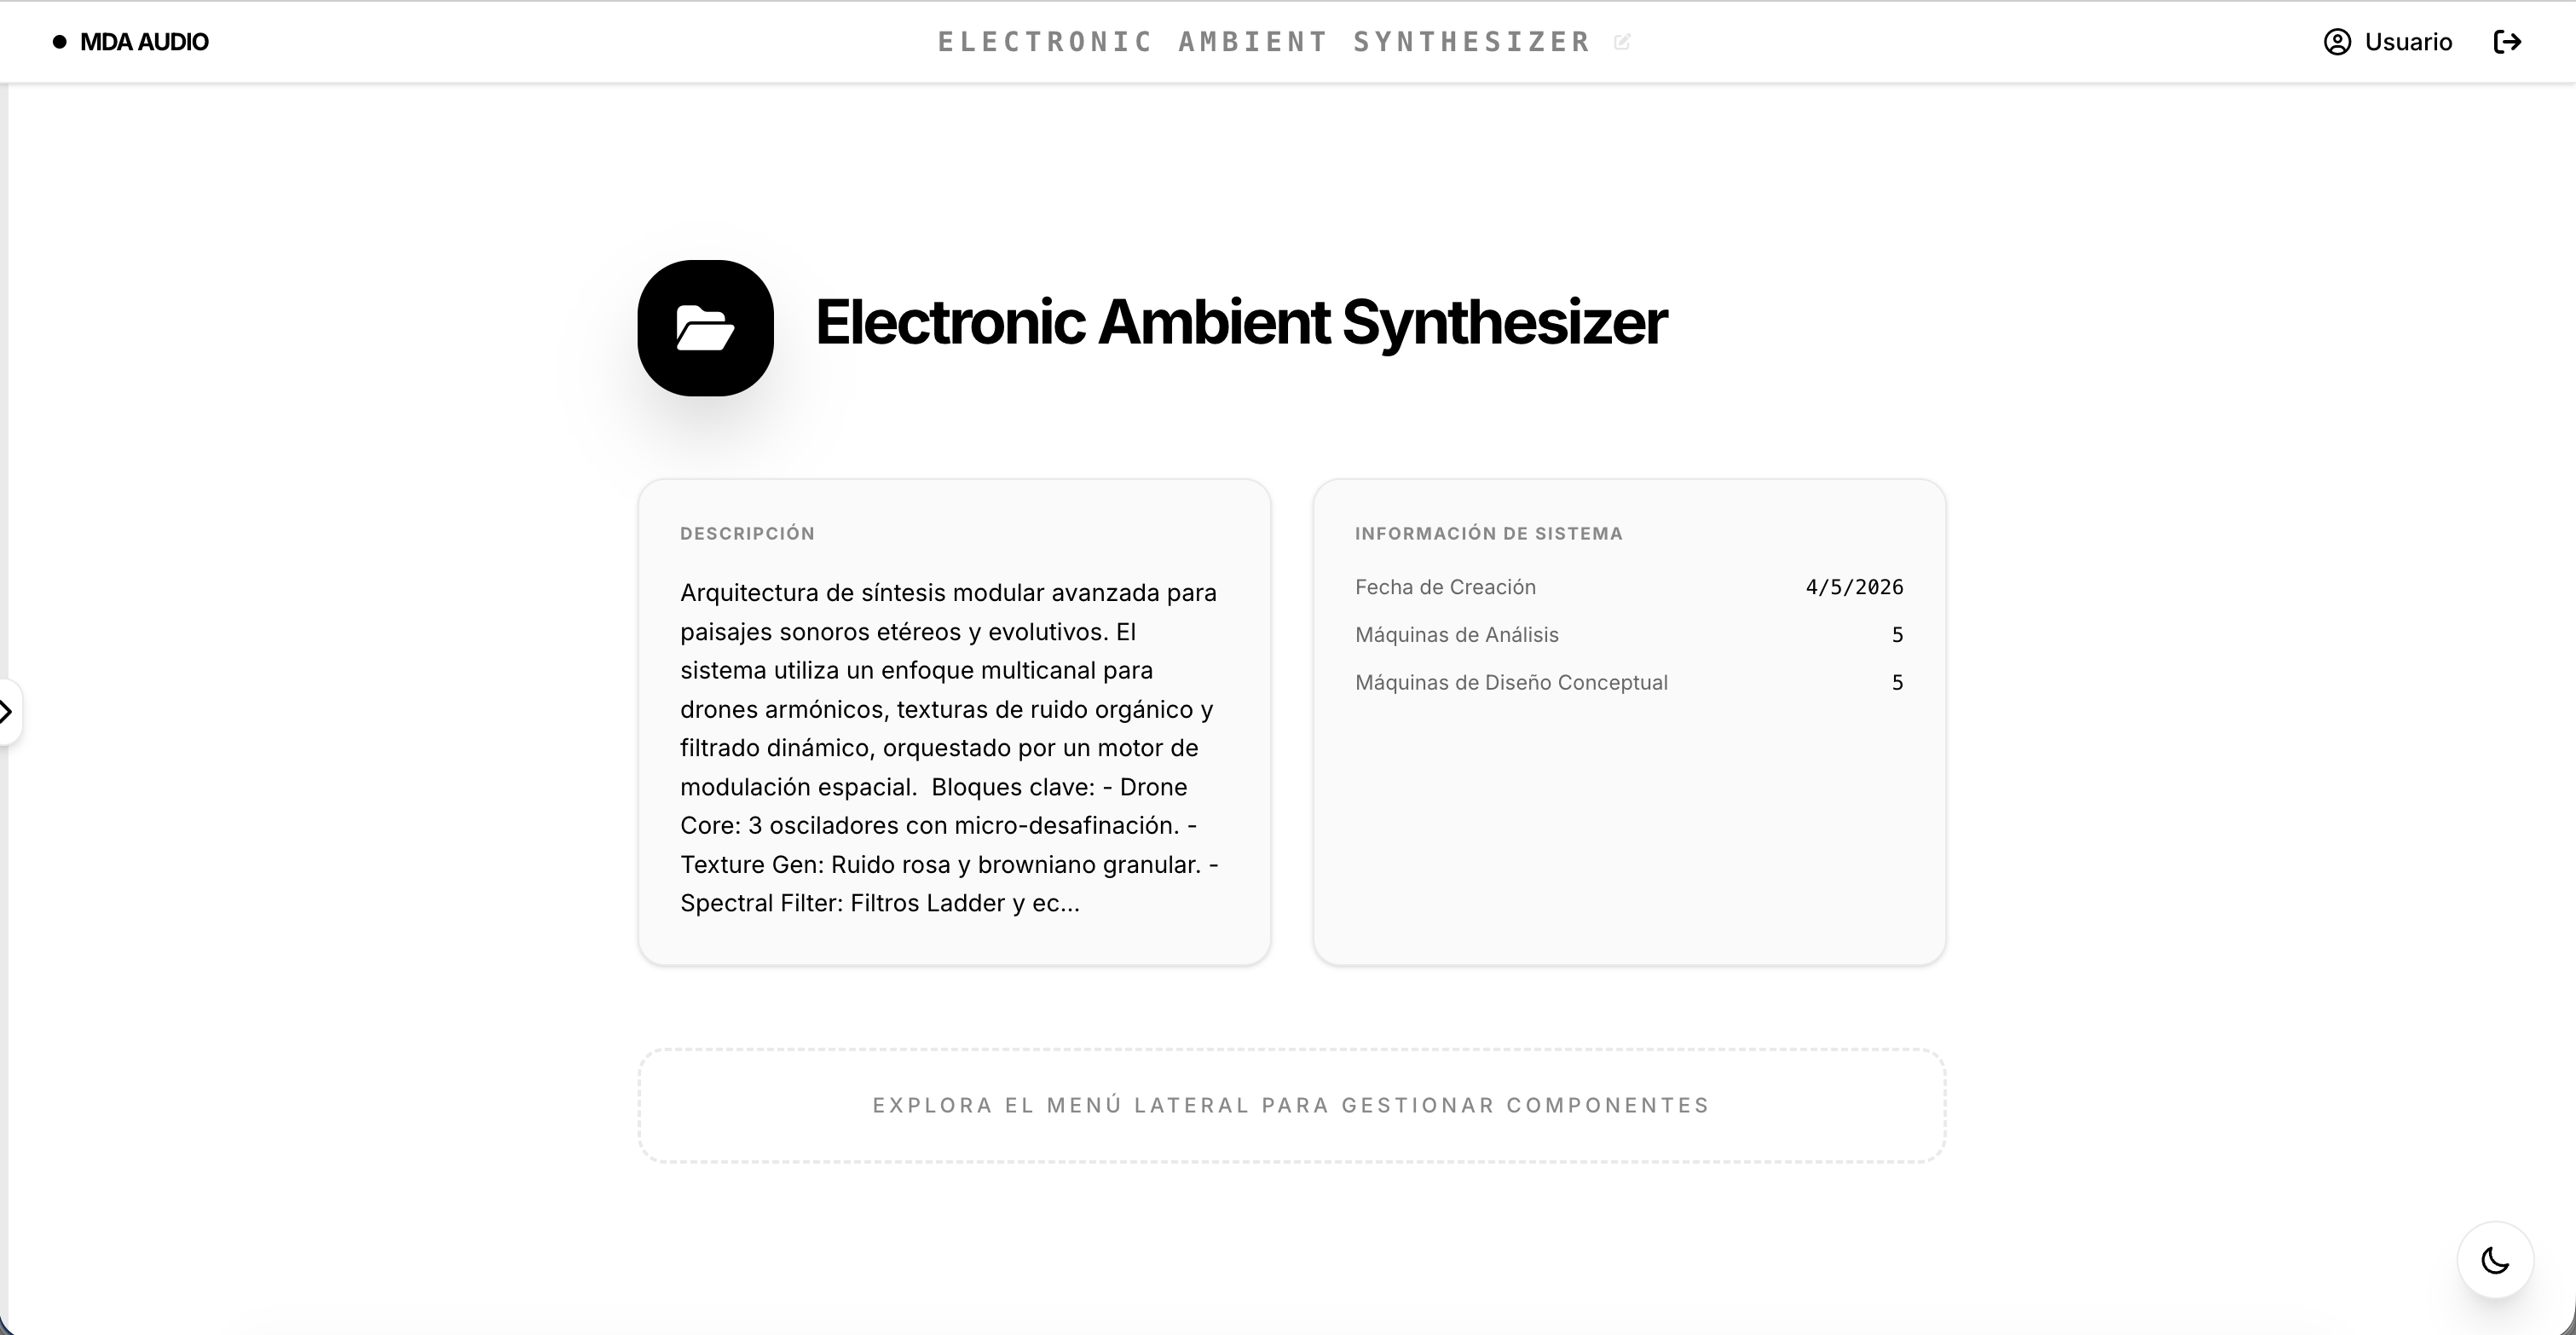
\includegraphics[width=0.6\textwidth]{imagenes/04_estructura/02_ocultacionExplorador.png}
    \caption{Botón para colapsar y ocultar el explorador lateral.}
\end{figure}

Para maximizar el espacio disponible en el área central, especialmente útil durante la edición de esquemas visuales complejos, el explorador puede ser colapsado y ocultado pulsando el botón situado en la parte superior izquierda.

\subsection{Barra Principal y Área de Trabajo}

\begin{figure}[!ht]
    \centering
    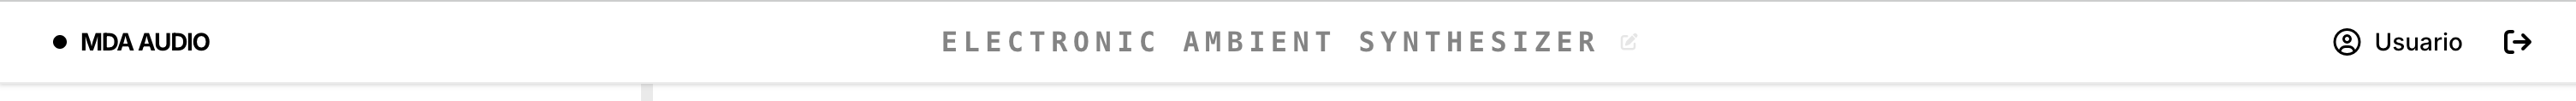
\includegraphics[width=\textwidth]{imagenes/04_estructura/04_barraPrincipal.png}
    \caption{Barra de herramientas principal.}
\end{figure}

La barra principal incluye, además de las opciones de gestión de sesión del usuario, botones de navegación como la vuelta al panel de proyectos y accesos a funcionalidades globales de exportación de modelos.

\begin{figure}[!ht]
    \centering
    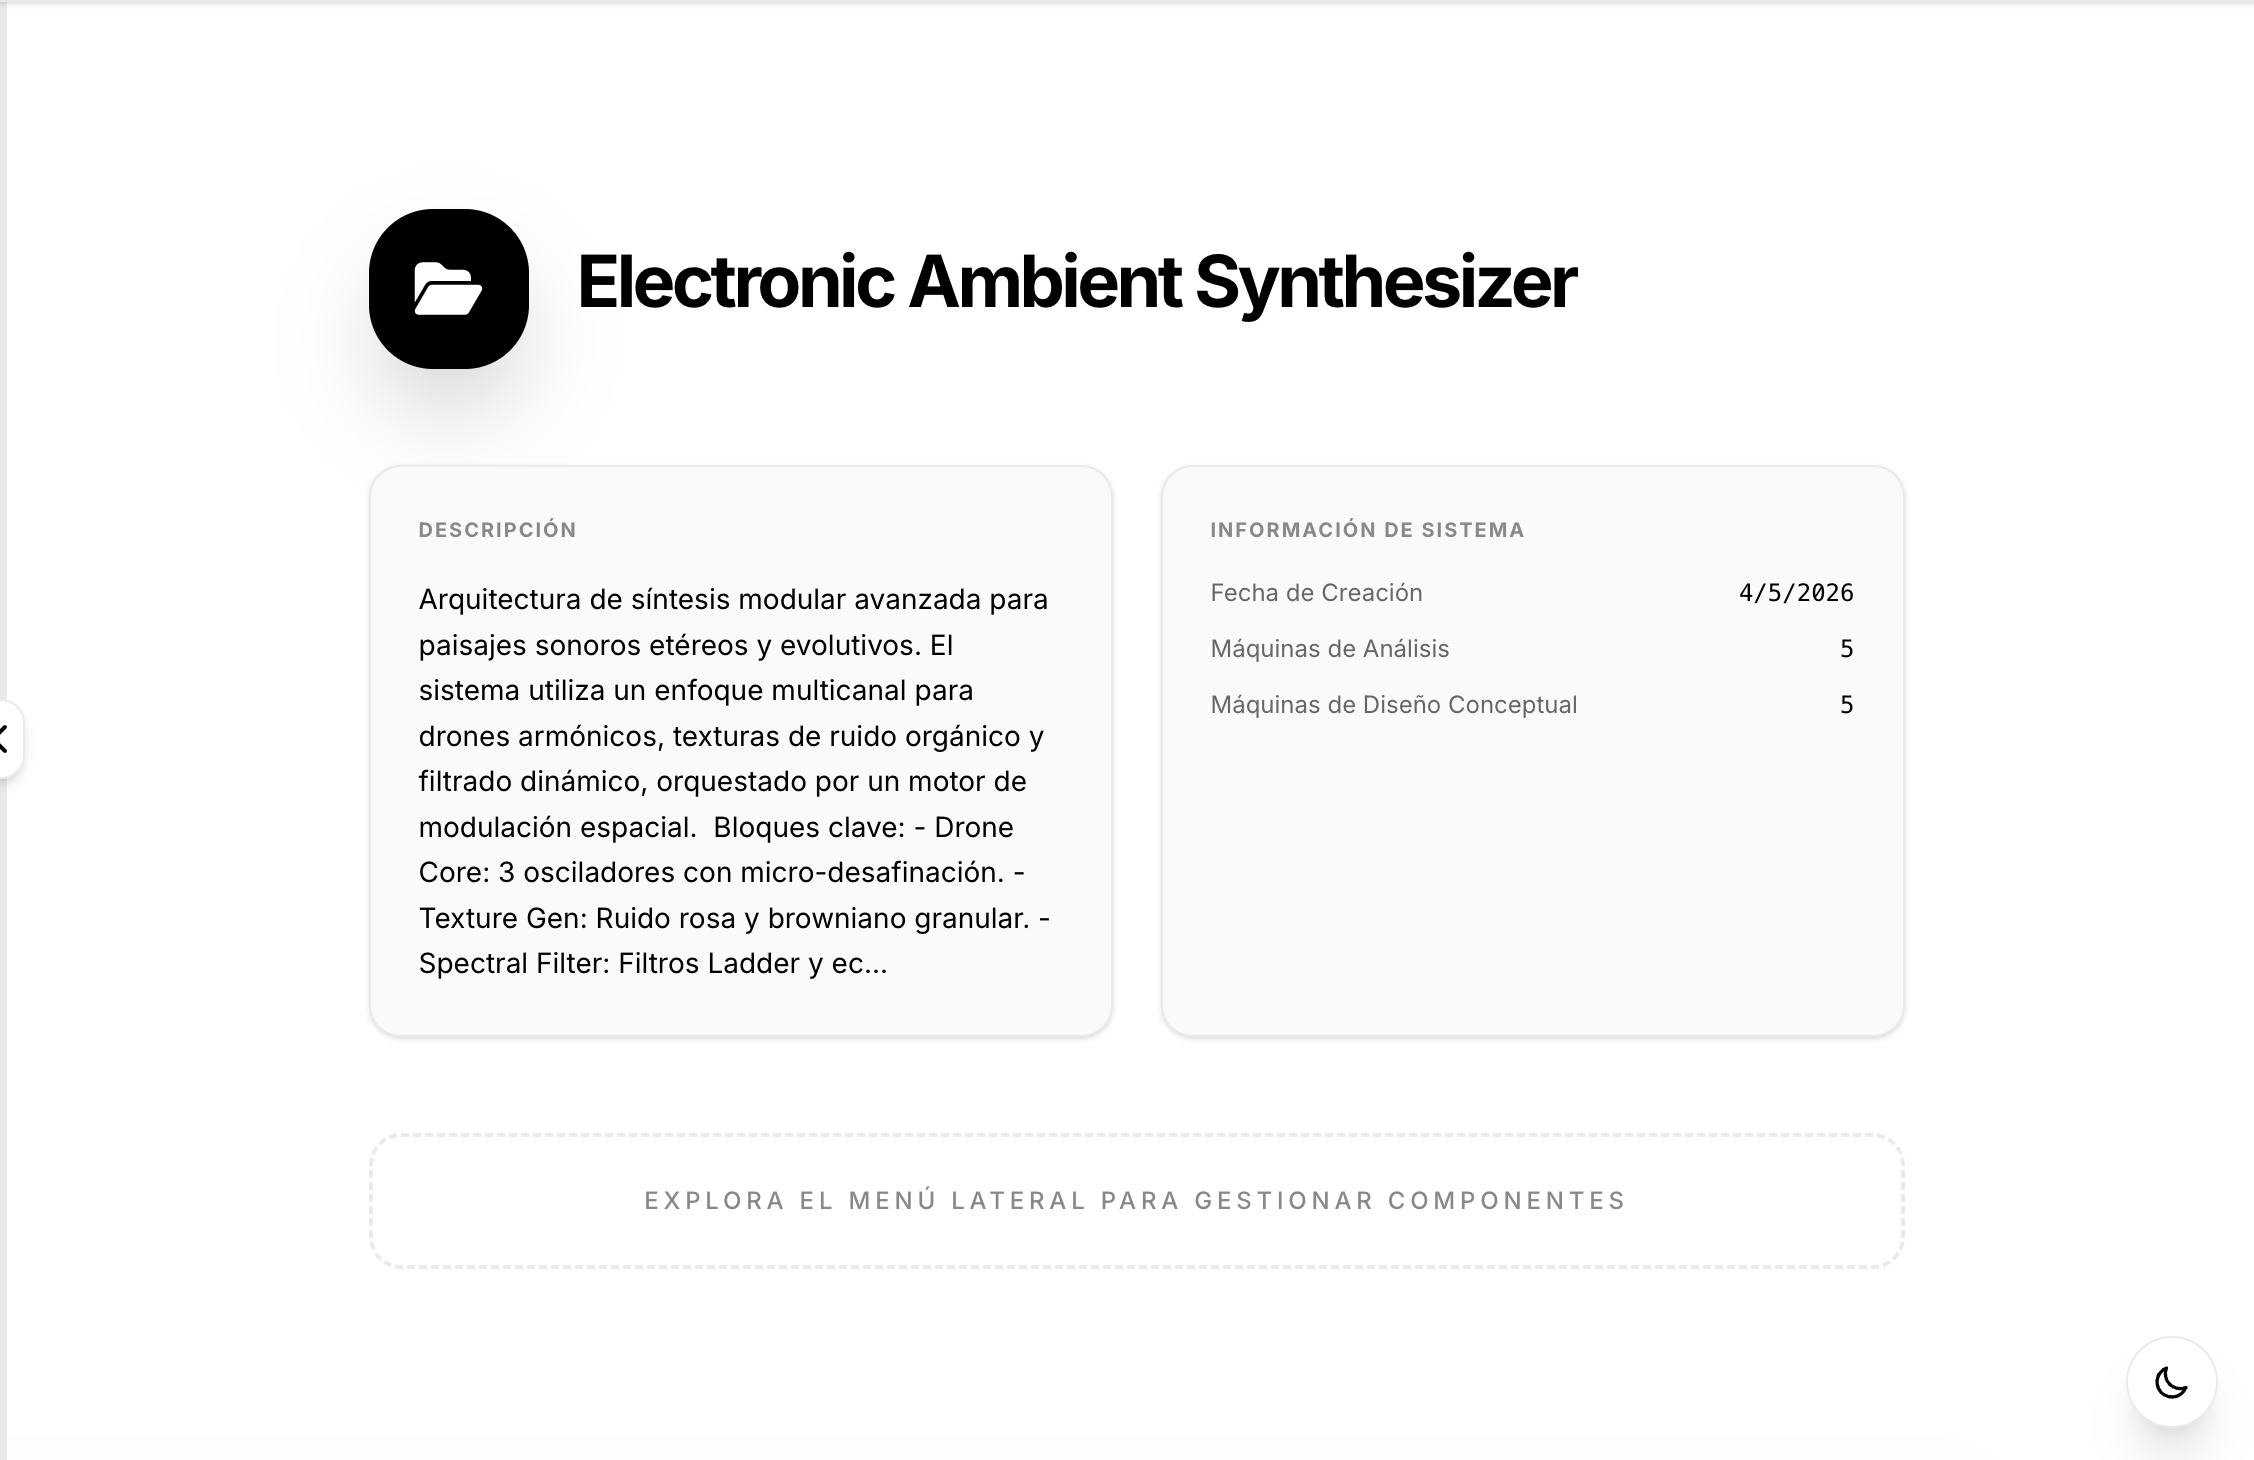
\includegraphics[width=\textwidth]{imagenes/04_estructura/05_objetosAbiertosEnElExplorador.png}
    \caption{Área de trabajo central con múltiples pestañas abiertas.}
\end{figure}

El área central utiliza un sistema de pestañas. A medida que el usuario selecciona elementos en el explorador, estos se abren en nuevas pestañas. Esto permite:
\begin{itemize}
    \item \textbf{Multitarea:} Mantener abiertos simultáneamente modelos de análisis, editores de diseño y grafos de relaciones.
    \item \textbf{Navegación Rápida:} Cambiar de contexto entre un modelo \textit{CIM} y uno \textit{PIM} rápidamente para verificar correspondencias conceptuales.
    \item \textbf{Cierre Selectivo:} Cerrar individualmente las pestañas que ya no se necesiten para mantener ordenado el espacio visual.
\end{itemize}

\chapter{Análisis Conceptual (CIM)}

\section{El Modelo Independiente de Computación}

El Análisis Conceptual representa el nivel superior en la abstracción \textit{MDAA}. En esta fase, el usuario define el \textit{CIM} (\textit{Computation Independent Model}), centrándose exclusivamente en los requerimientos lógicos del dominio musical, sin considerar aún aspectos tecnológicos de su futura implementación.

\begin{figure}[!ht]
    \centering
    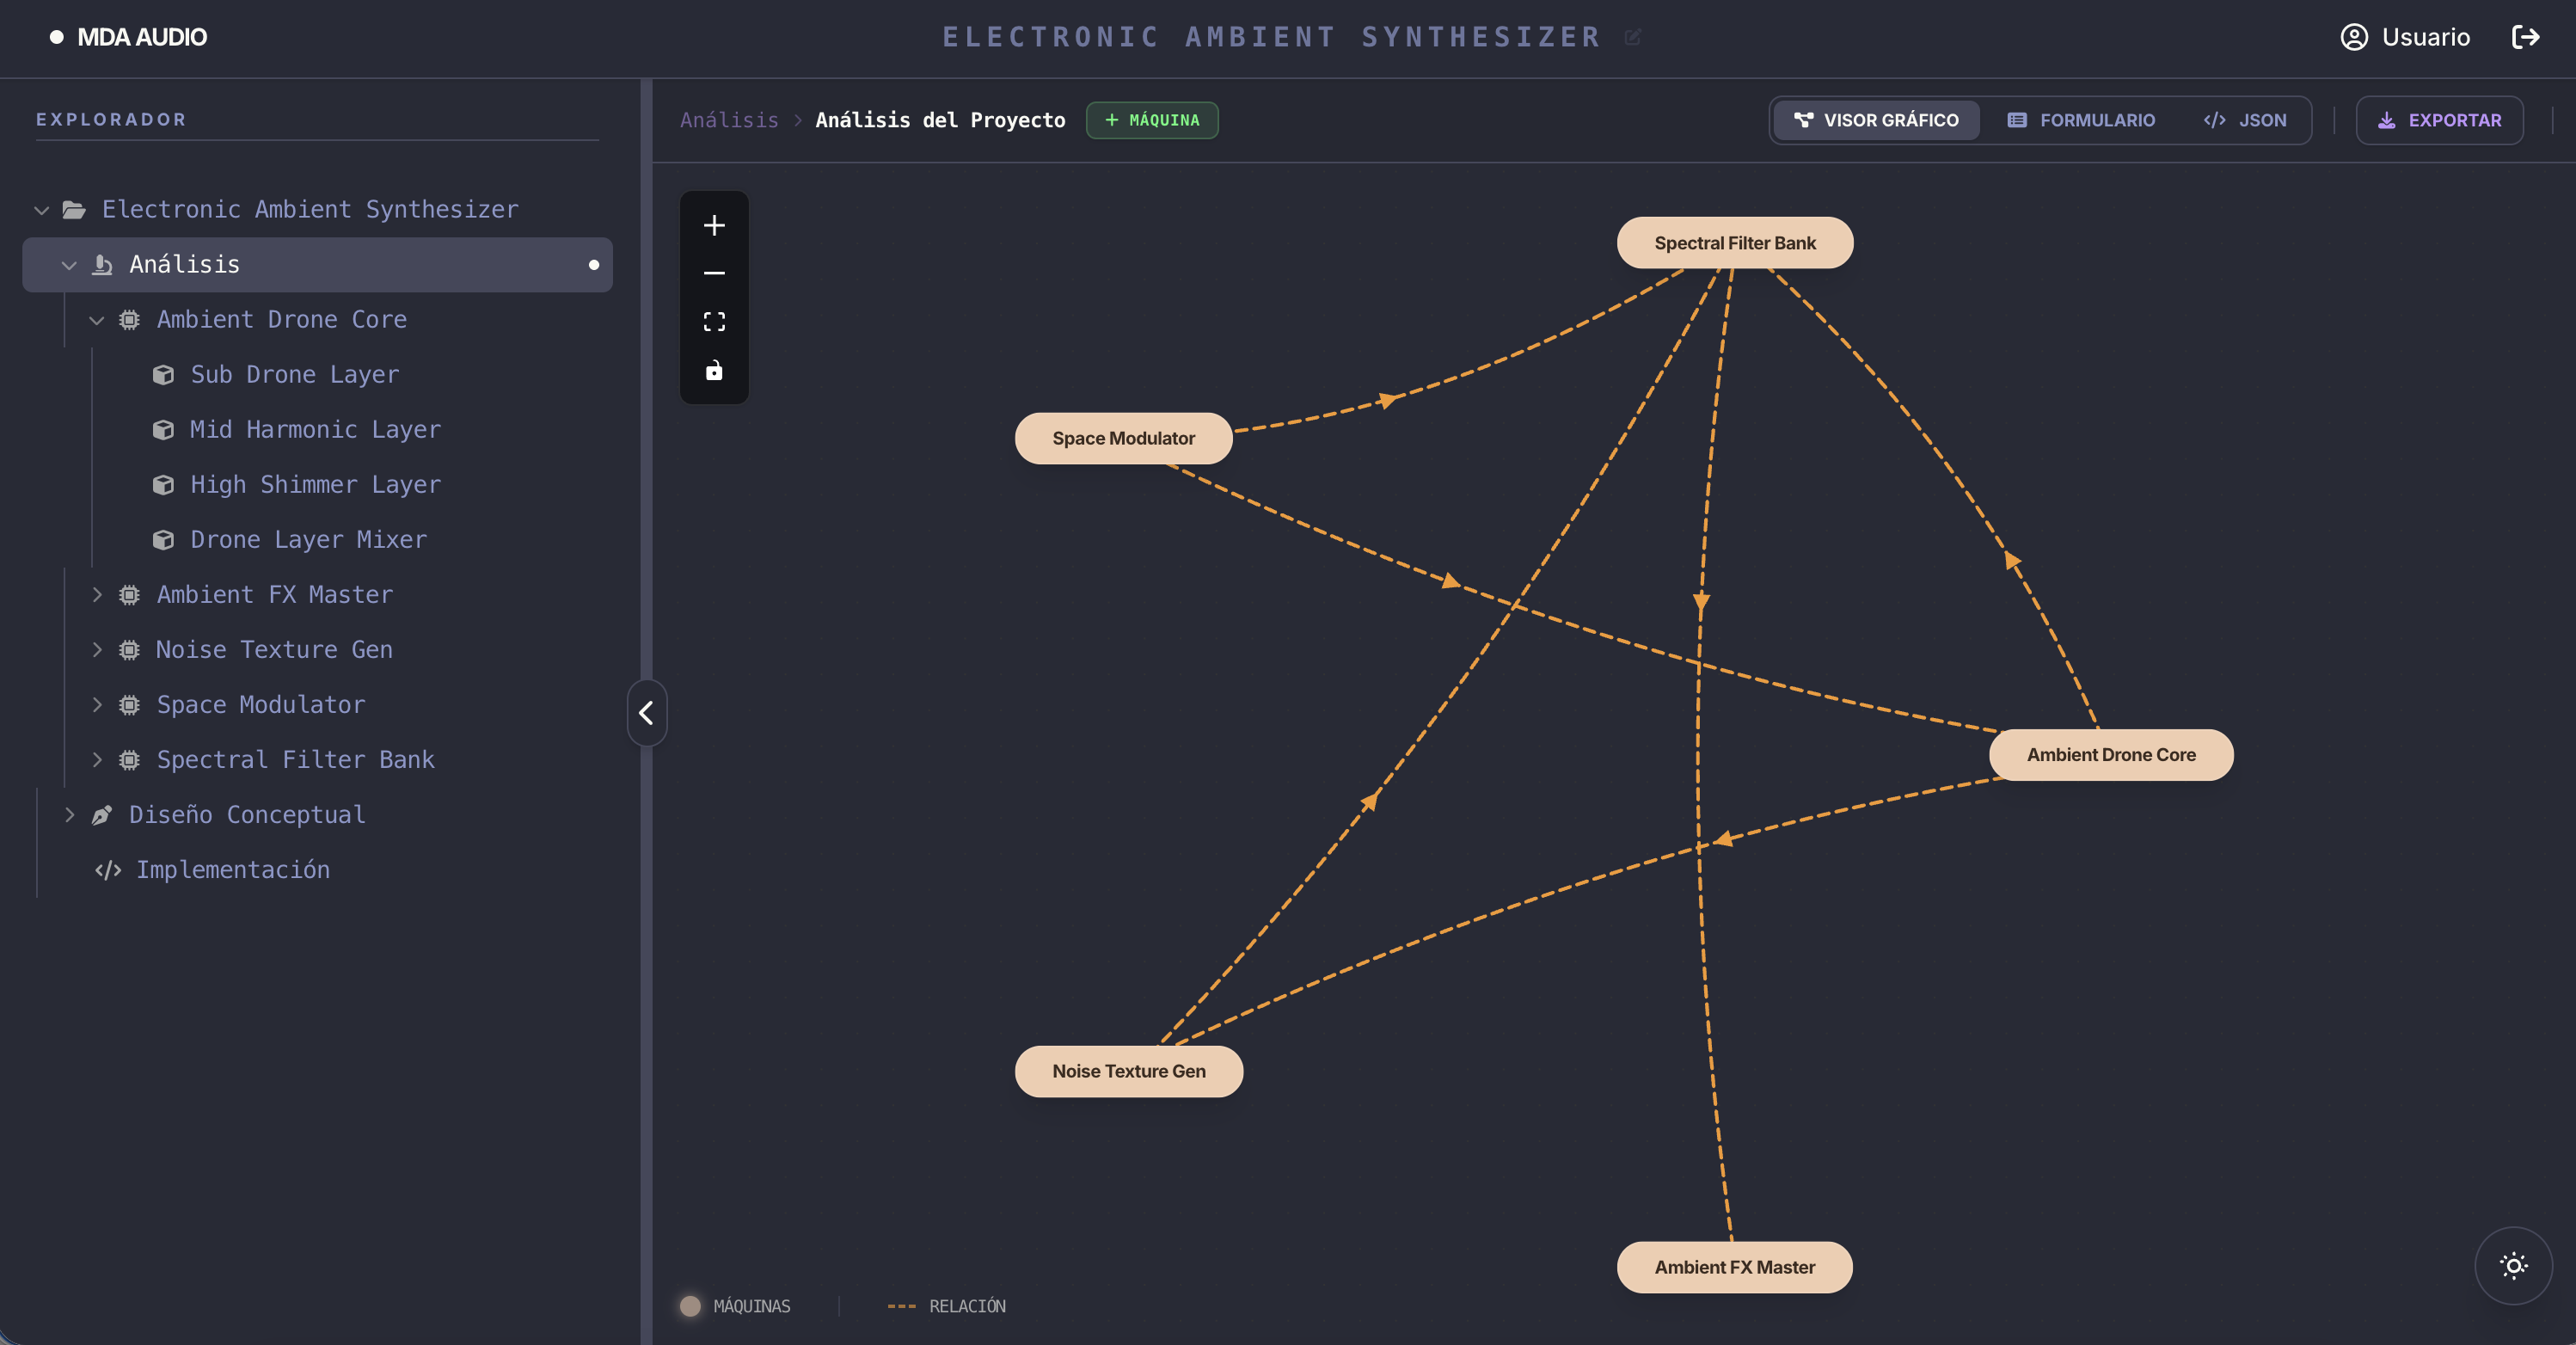
\includegraphics[width=\textwidth]{imagenes/05_analisis/01_pantallaPrincipalAnalisis.png}
    \caption{Vista general del entorno de Análisis Conceptual.}
\end{figure}

Al seleccionar la rama de Análisis Conceptual en el explorador, se abre el área de trabajo dedicada al entorno \textit{CIM}. Esta interfaz facilita la gestión de las entidades principales (las máquinas conceptuales) y la definición de las interacciones lógicas entre ellas.

\begin{figure}[!ht]
    \centering
    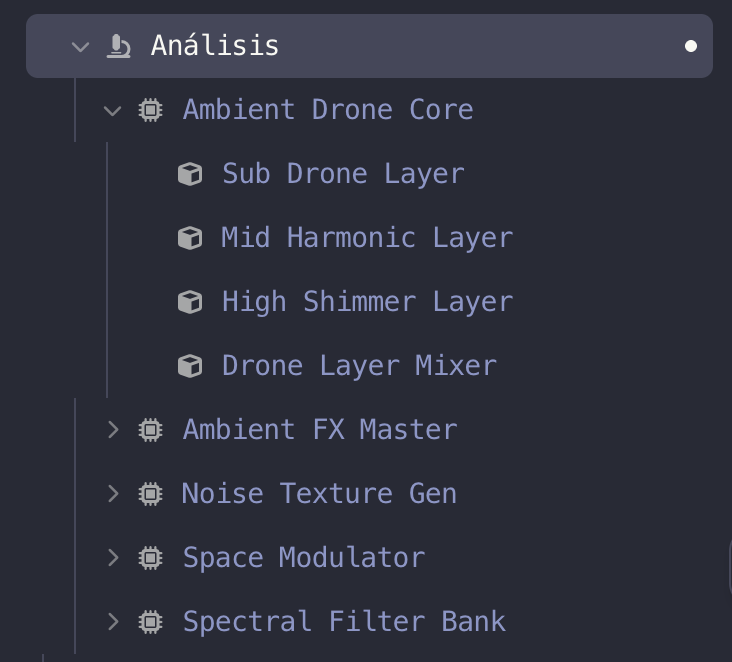
\includegraphics[width=0.4\textwidth]{imagenes/05_analisis/02_exploradorAnalisis.png}
    \caption{Detalle del nodo de Análisis Conceptual en el explorador.}
\end{figure}

El nodo raíz de \textit{CIM} actúa como contenedor global. Desplegando esta rama, el usuario puede navegar hacia la configuración orquestal (relaciones) o acceder a la definición específica de cada máquina conceptual individual.

\begin{figure}[!ht]
    \centering
    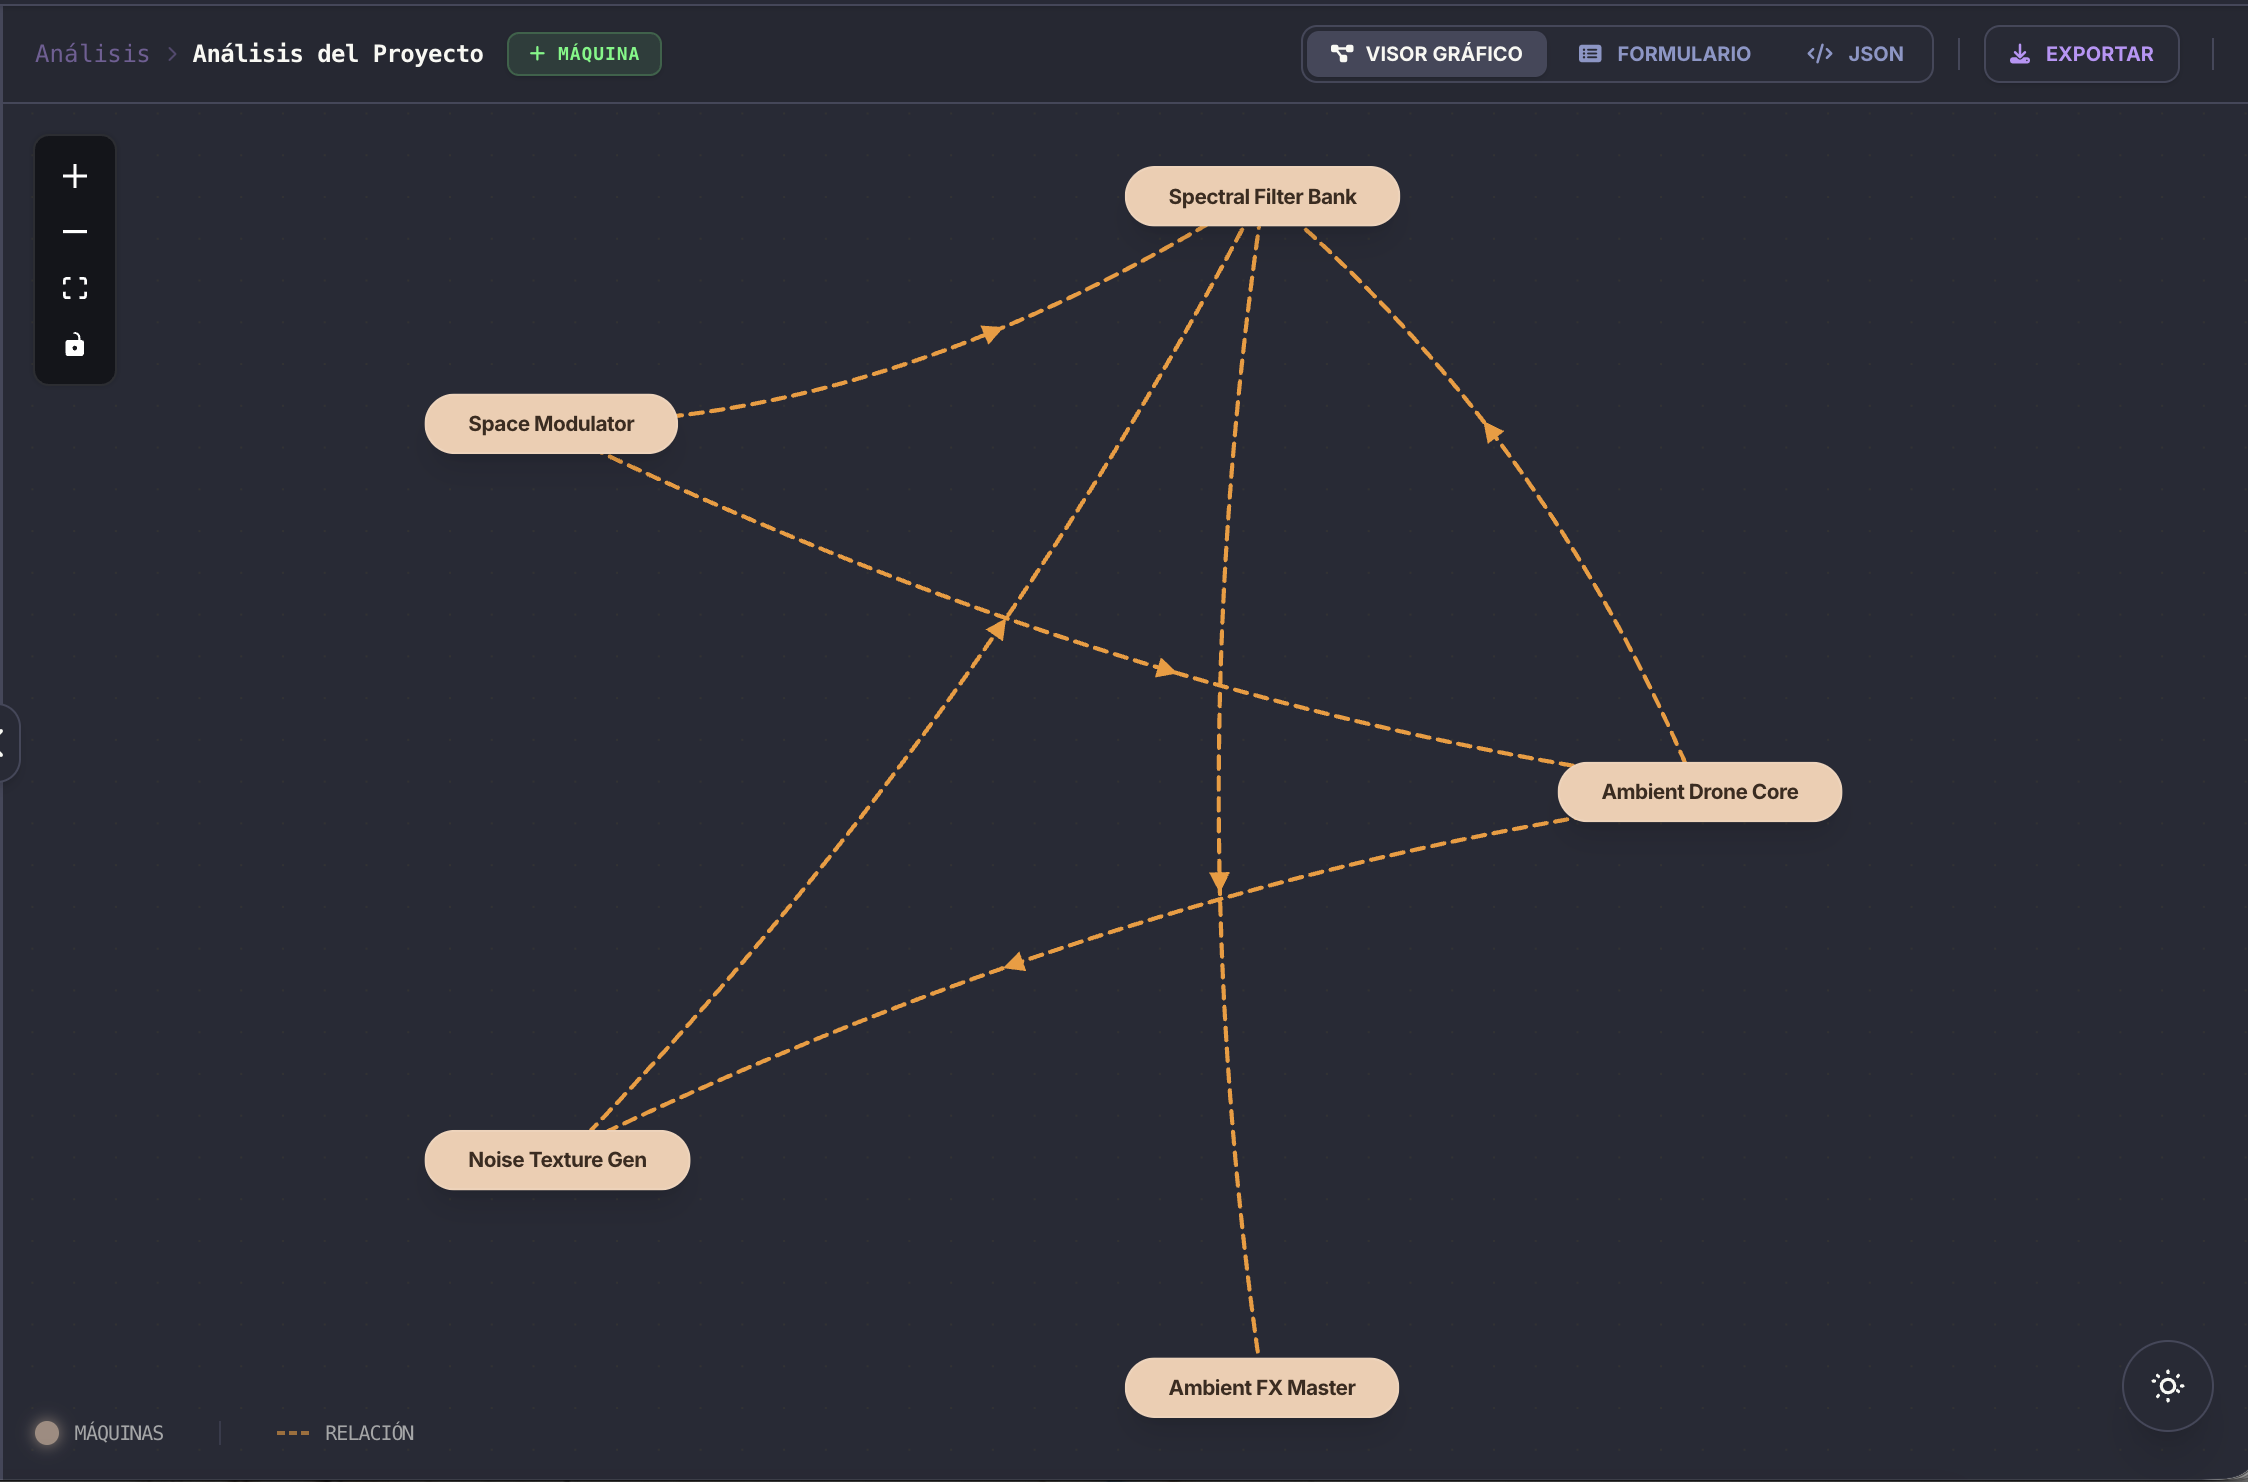
\includegraphics[width=\textwidth]{imagenes/05_analisis/03_pantallaVistaDelNodoAnalisis.png}
    \caption{Pantalla de vista detallada al seleccionar el nodo raíz de Análisis Conceptual.}
\end{figure}

La pantalla principal del nivel \textit{CIM} centraliza las herramientas para la gestión estructural. Su propósito es definir la red de componentes musicales.

\subsection{Creación de Máquinas Conceptuales}

\begin{figure}[!ht]
    \centering
    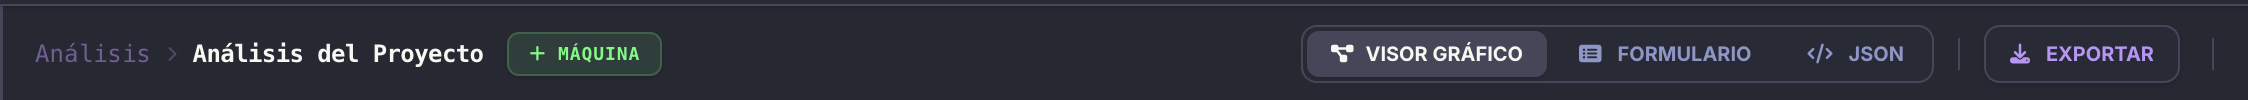
\includegraphics[width=0.4\textwidth]{imagenes/05_analisis/04_botoneraAccionAnalisis.png}
    \caption{Botonera de acciones globales del Análisis Conceptual.}
\end{figure}

\begin{figure}[!ht]
    \centering
    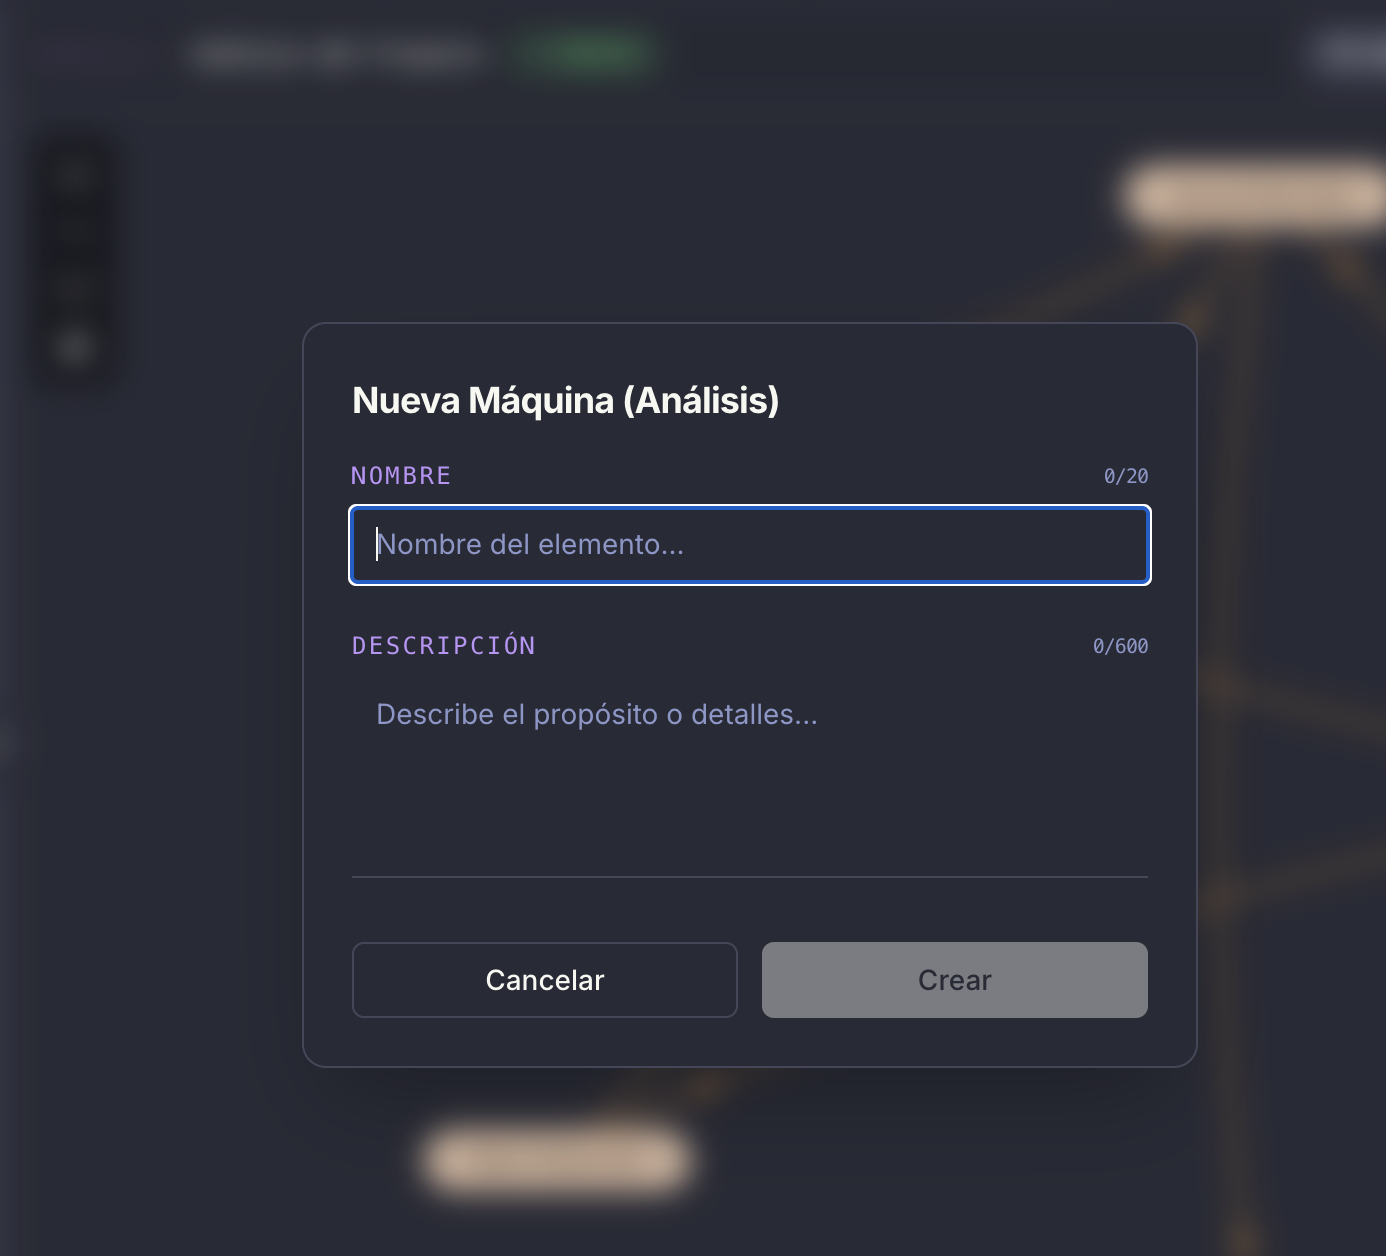
\includegraphics[width=0.6\textwidth]{imagenes/05_analisis/05_crearMaquina.png}
    \caption{Formulario para la creación de una nueva máquina CIM.}
\end{figure}

Desde la botonera superior es posible invocar la creación de nuevas máquinas. Este formulario solicita información esencial, como el identificador único, para instanciar el elemento dentro del modelo del lenguaje \textit{DSL}. Una vez salvada, la nueva máquina se incorpora al árbol del explorador.

\section{Gestión de Relaciones CIM}

Para establecer la conectividad conceptual entre las máquinas, la plataforma ofrece tres modos de trabajo adaptados a distintos perfiles de usuario.

\begin{figure}[!ht]
    \centering
    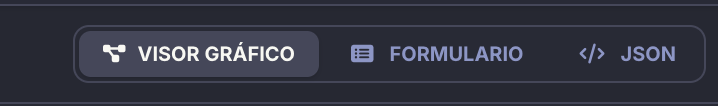
\includegraphics[width=0.5\textwidth]{imagenes/05_analisis/06_botoneraVistasAnalisis.png}
    \caption{Selector de vistas: Visor Gráfico, Formulario y Código JSON.}
\end{figure}

La botonera de vistas permite alternar instantáneamente entre la representación gráfica, el editor basado en formularios y el editor de código avanzado.

\subsection{Visor Gráfico}

\begin{figure}[!ht]
    \centering
    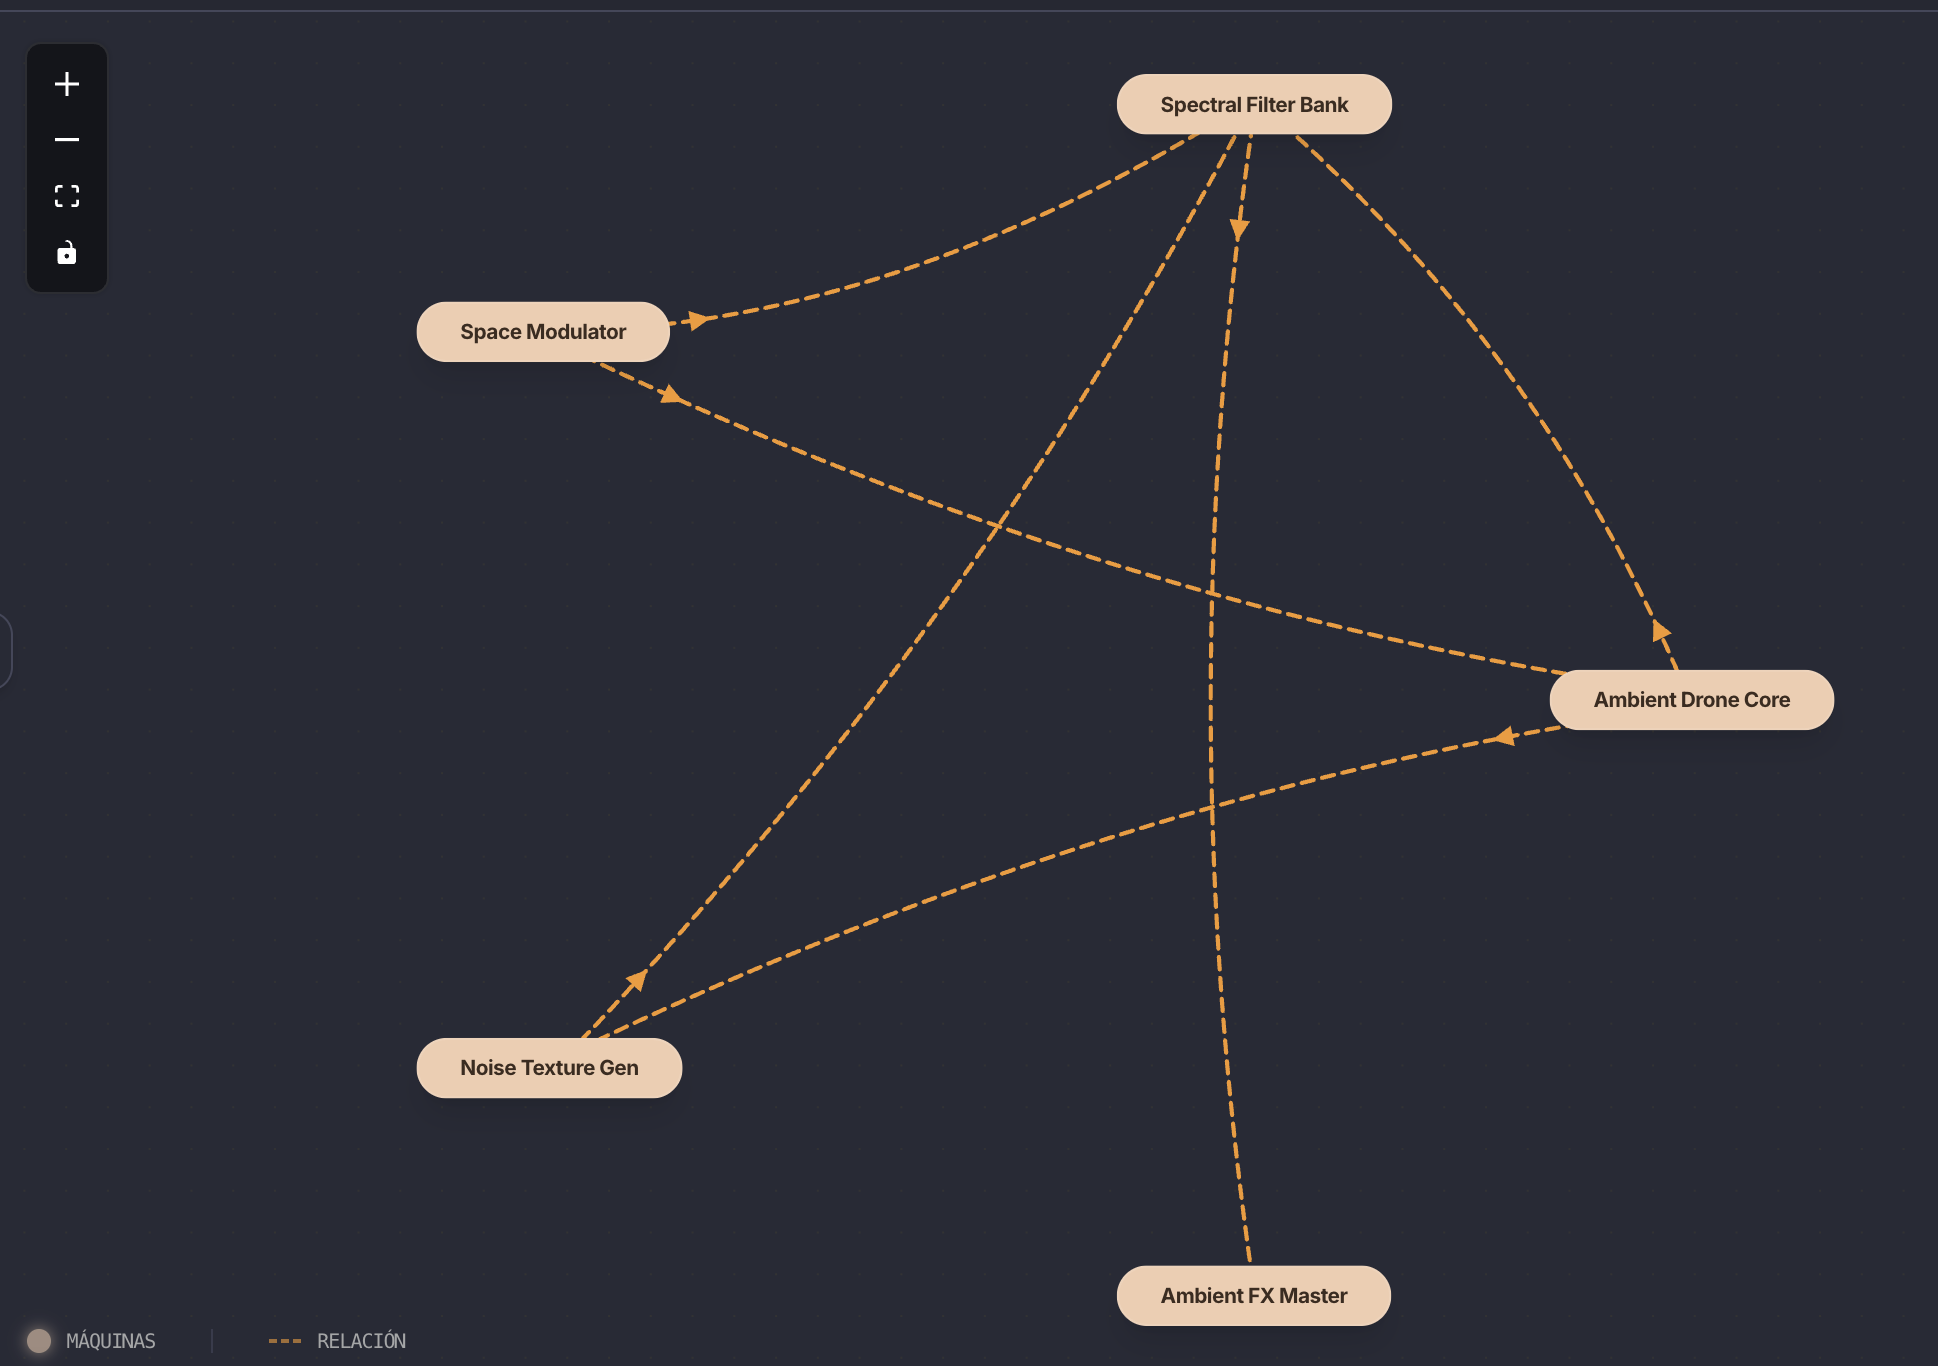
\includegraphics[width=\textwidth]{imagenes/05_analisis/07_grafoRelacionesAnalisis.png}
    \caption{Representación en forma de grafo interactivo de las relaciones entre máquinas.}
\end{figure}

El visor muestra un grafo dinámico. Los nodos simbolizan las máquinas conceptuales, mientras que las aristas direccionadas exponen el flujo de la señal o la lógica de control.

\begin{figure}[!ht]
    \centering
    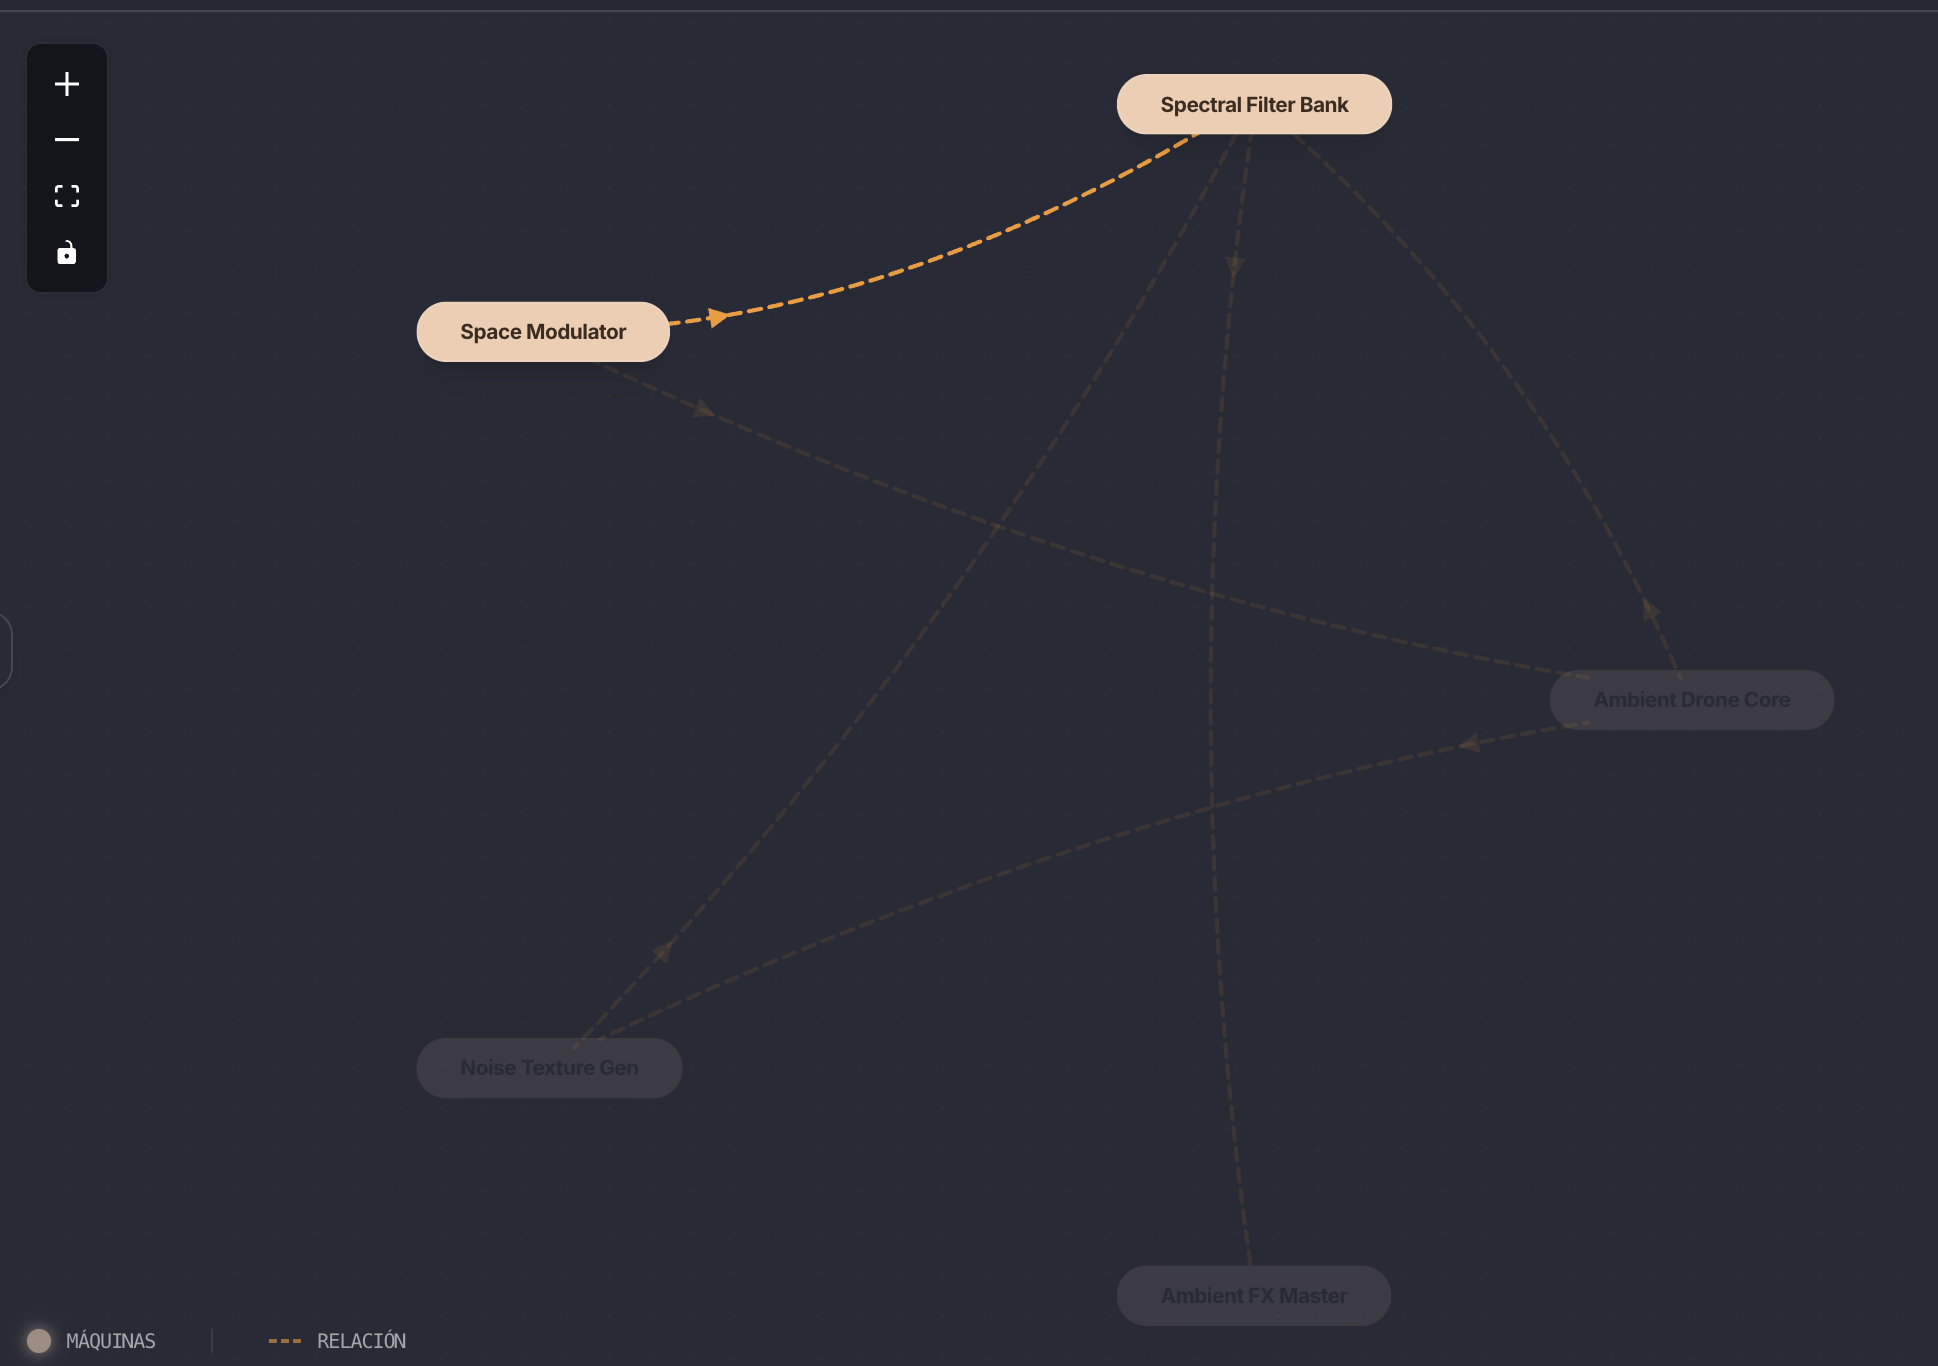
\includegraphics[width=\textwidth]{imagenes/05_analisis/08_aristaGrafoPulsado.png}
    \caption{Inspección de metadatos al seleccionar una relación (arista).}
\end{figure}

\begin{figure}[!ht]
    \centering
    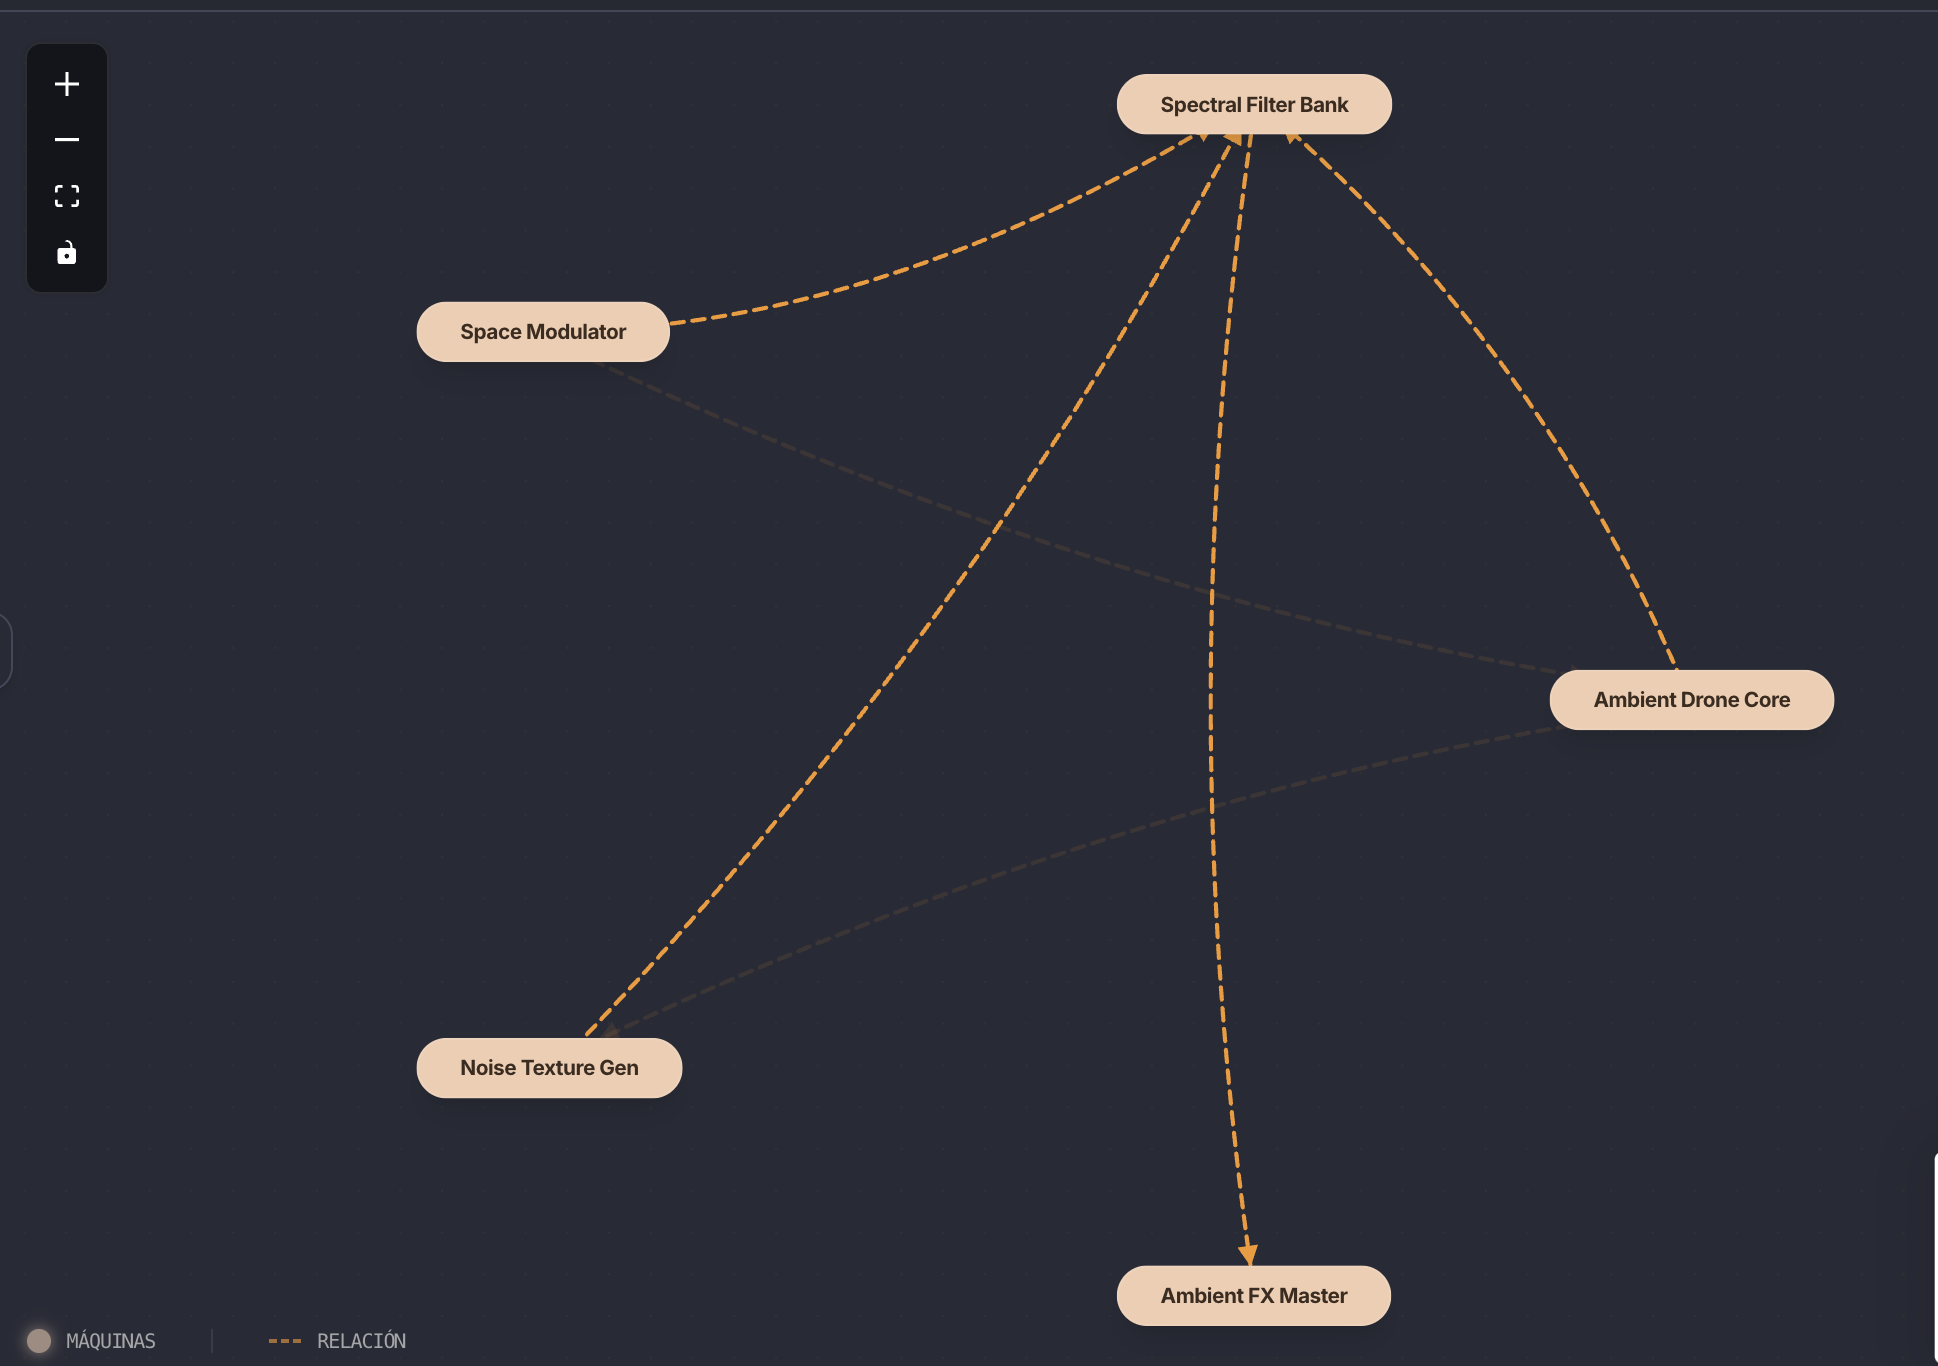
\includegraphics[width=\textwidth]{imagenes/05_analisis/09_nodoGrafoPulsado.png}
    \caption{Inspección de metadatos al seleccionar una máquina (nodo).}
\end{figure}

La interfaz es plenamente interactiva. Al pulsar sobre cualquier componente topológico (nodo o arista), se revela un panel de información detallada, permitiendo al usuario revisar la arquitectura sin analizar directamente el código subyacente.

\subsection{Editores de Relaciones}

\begin{figure}[!ht]
    \centering
    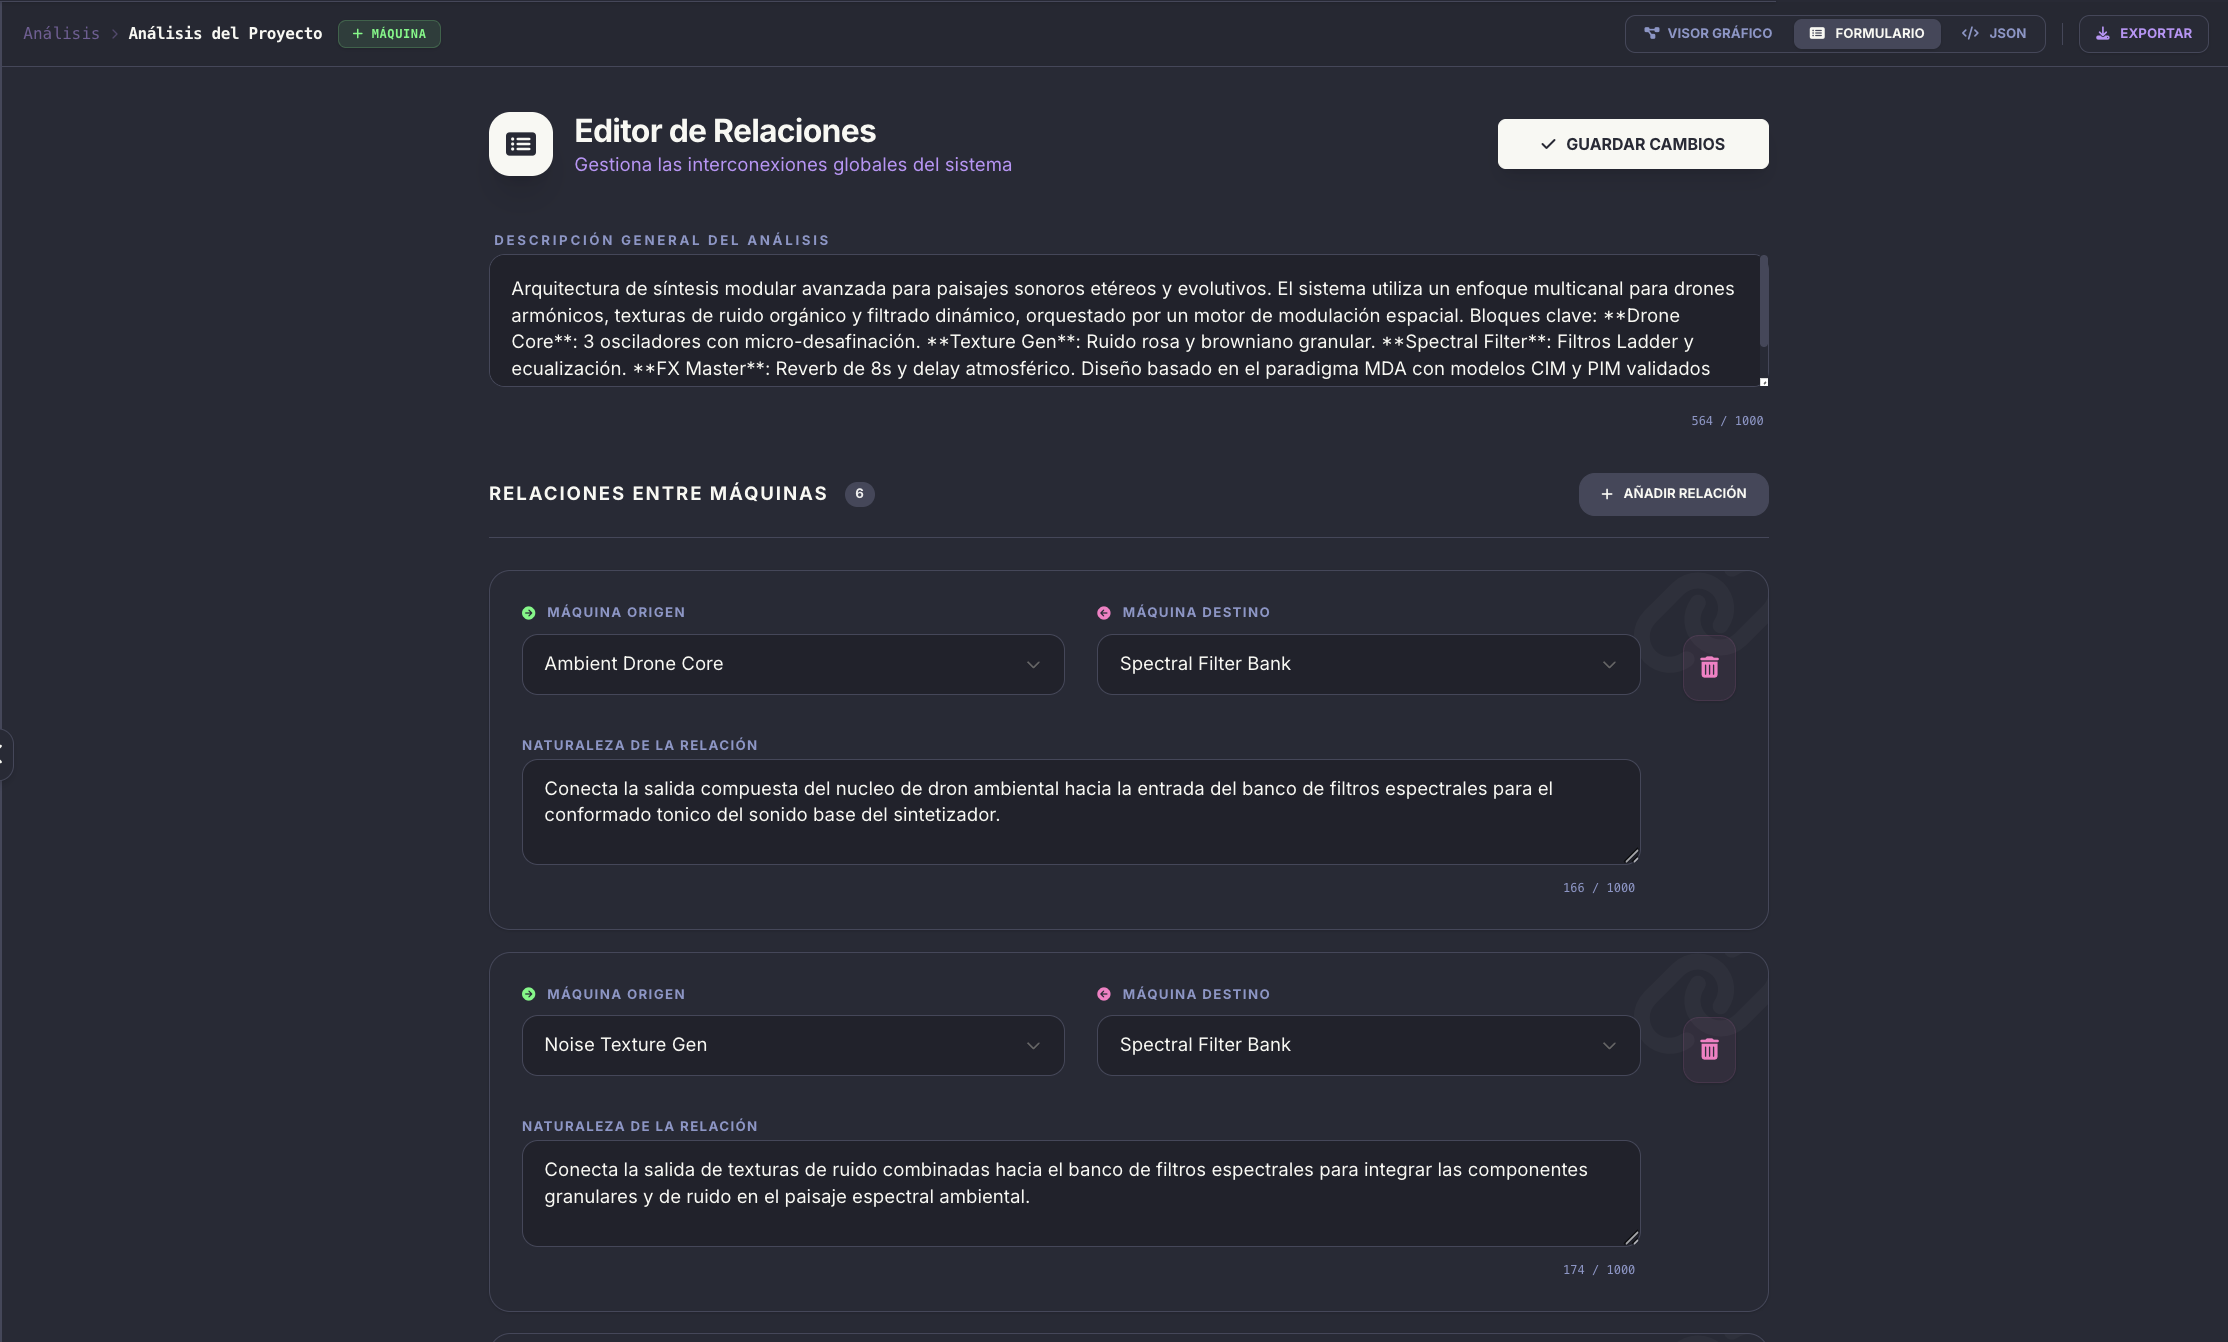
\includegraphics[width=\textwidth]{imagenes/05_analisis/10_editorFormularioRelacionesCim.png}
    \caption{Editor de relaciones mediante interfaz de formulario.}
\end{figure}

Para una edición asistida y visual, el editor de formularios posibilita la creación y alteración de enlaces seleccionando orígenes y destinos a través de selectores amigables.

\begin{figure}[!ht]
    \centering
    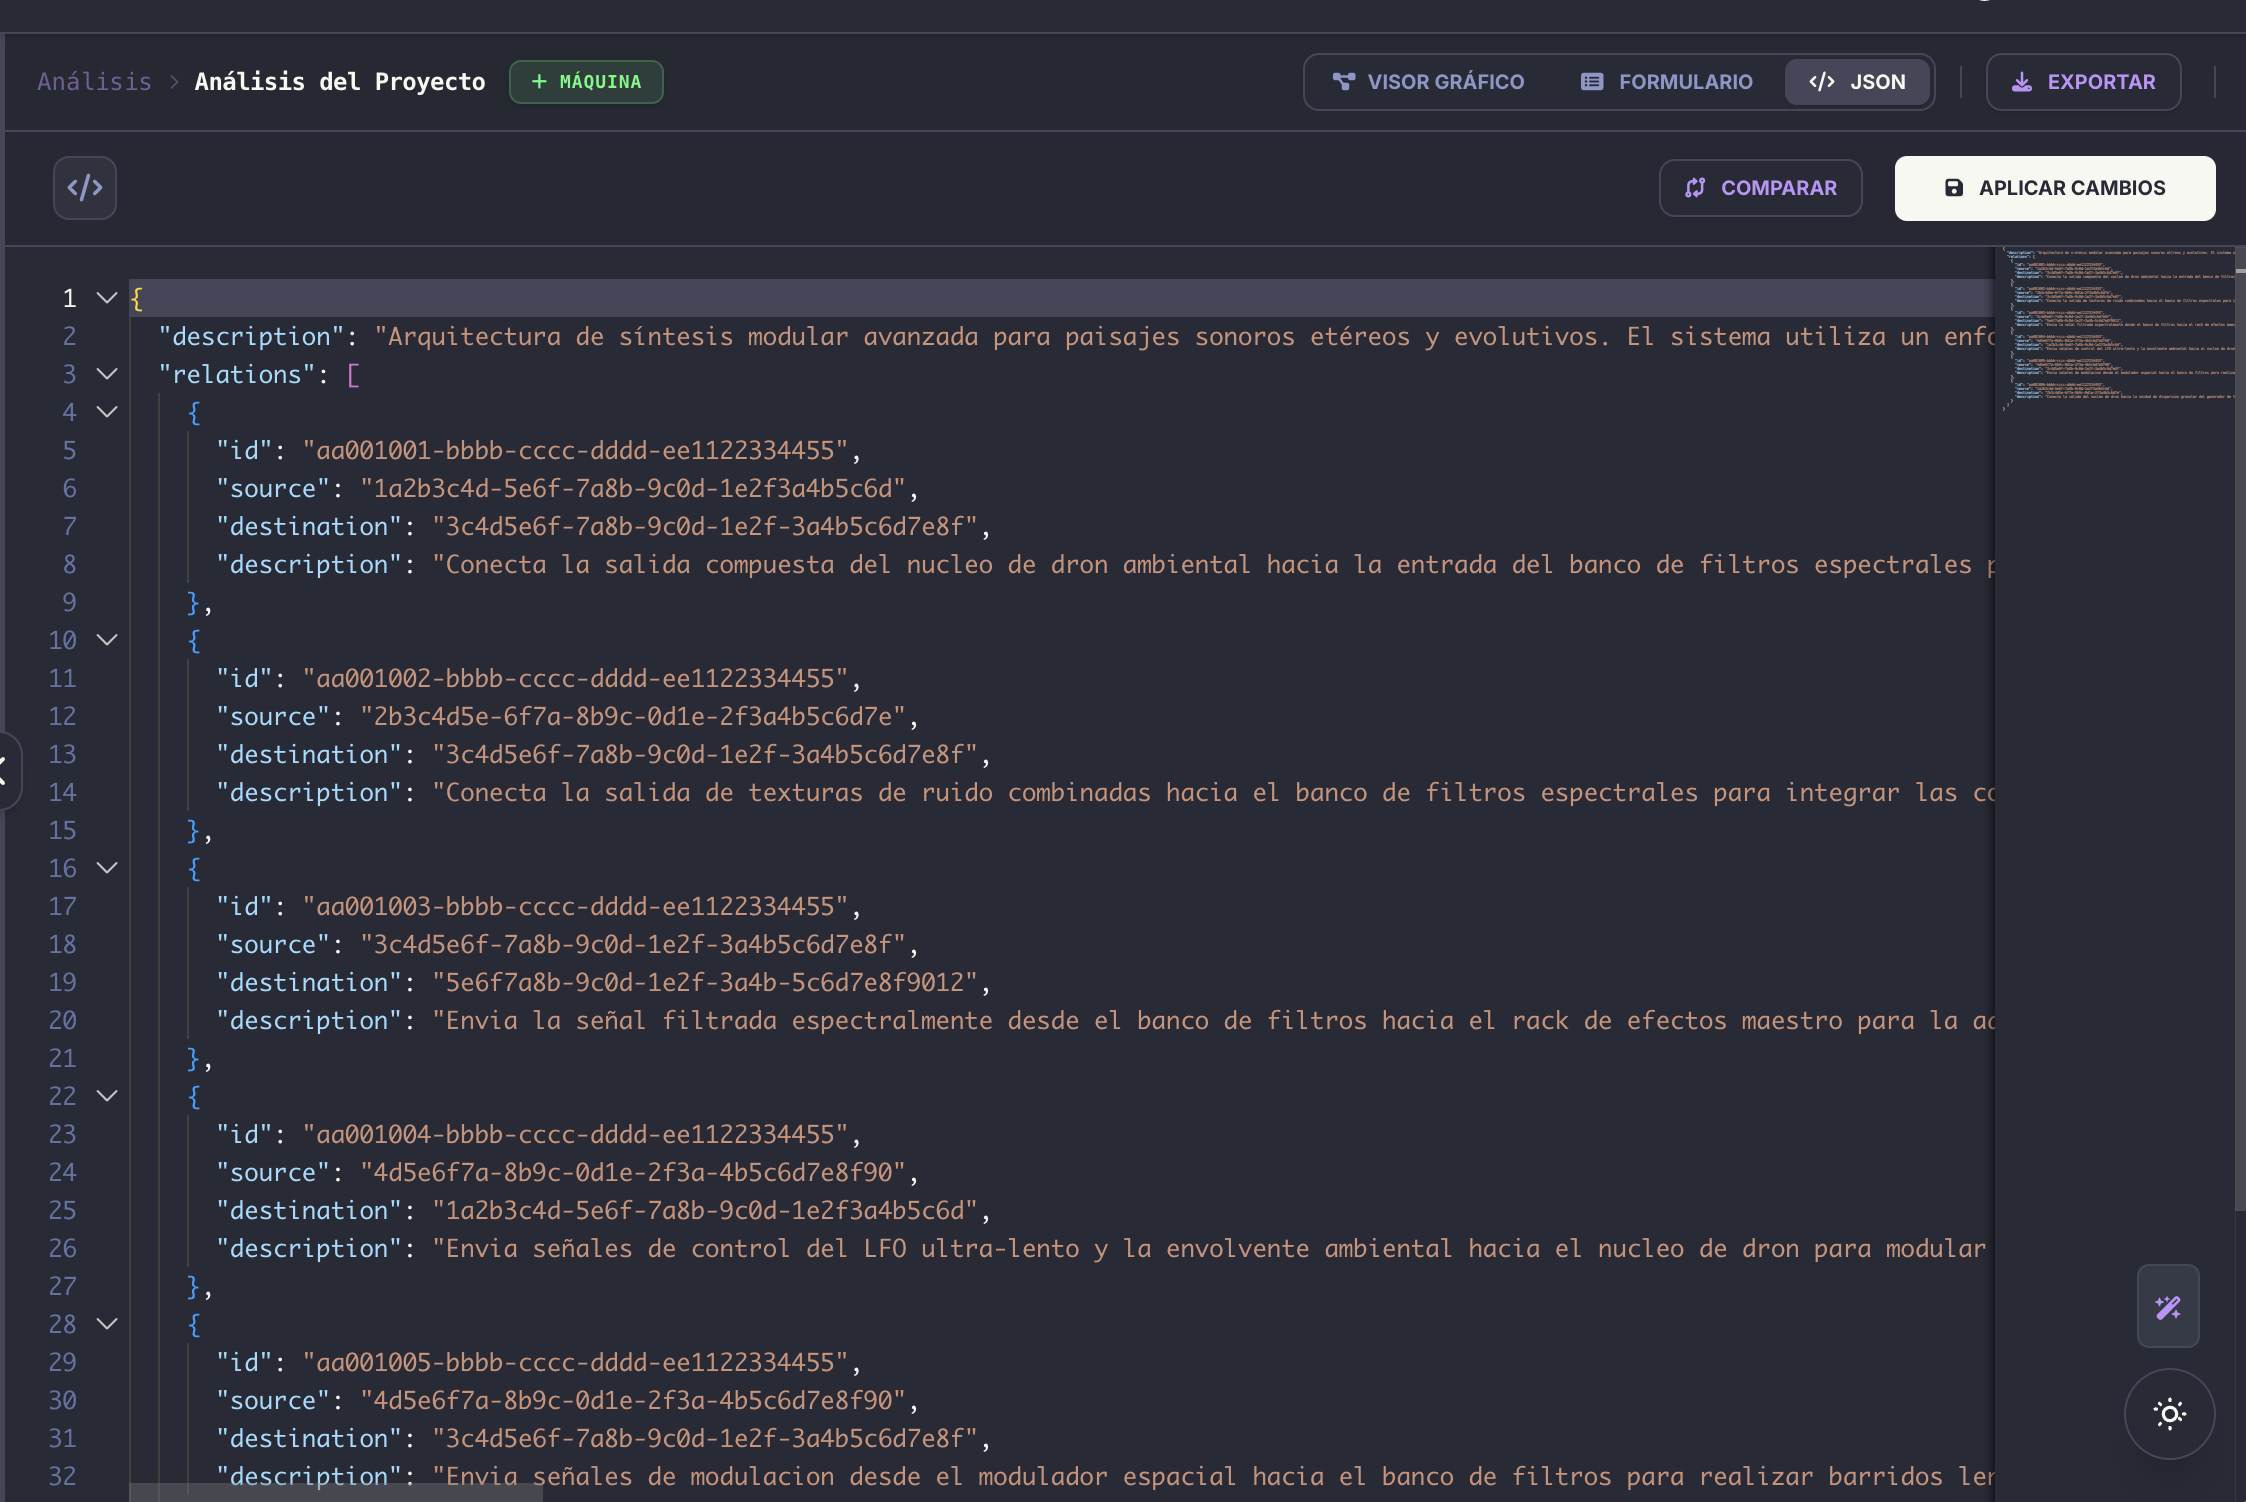
\includegraphics[width=\textwidth]{imagenes/05_analisis/11_edicionJsonRelacionesCim.png}
    \caption{Editor avanzado de código fuente (JSON) para las relaciones CIM.}
\end{figure}

Los usuarios familiarizados con la especificación \textit{DSL} pueden trabajar directamente sobre el código \textit{JSON}. Este editor incluye autocompletado y resaltado sintáctico.

\begin{figure}[!ht]
    \centering
    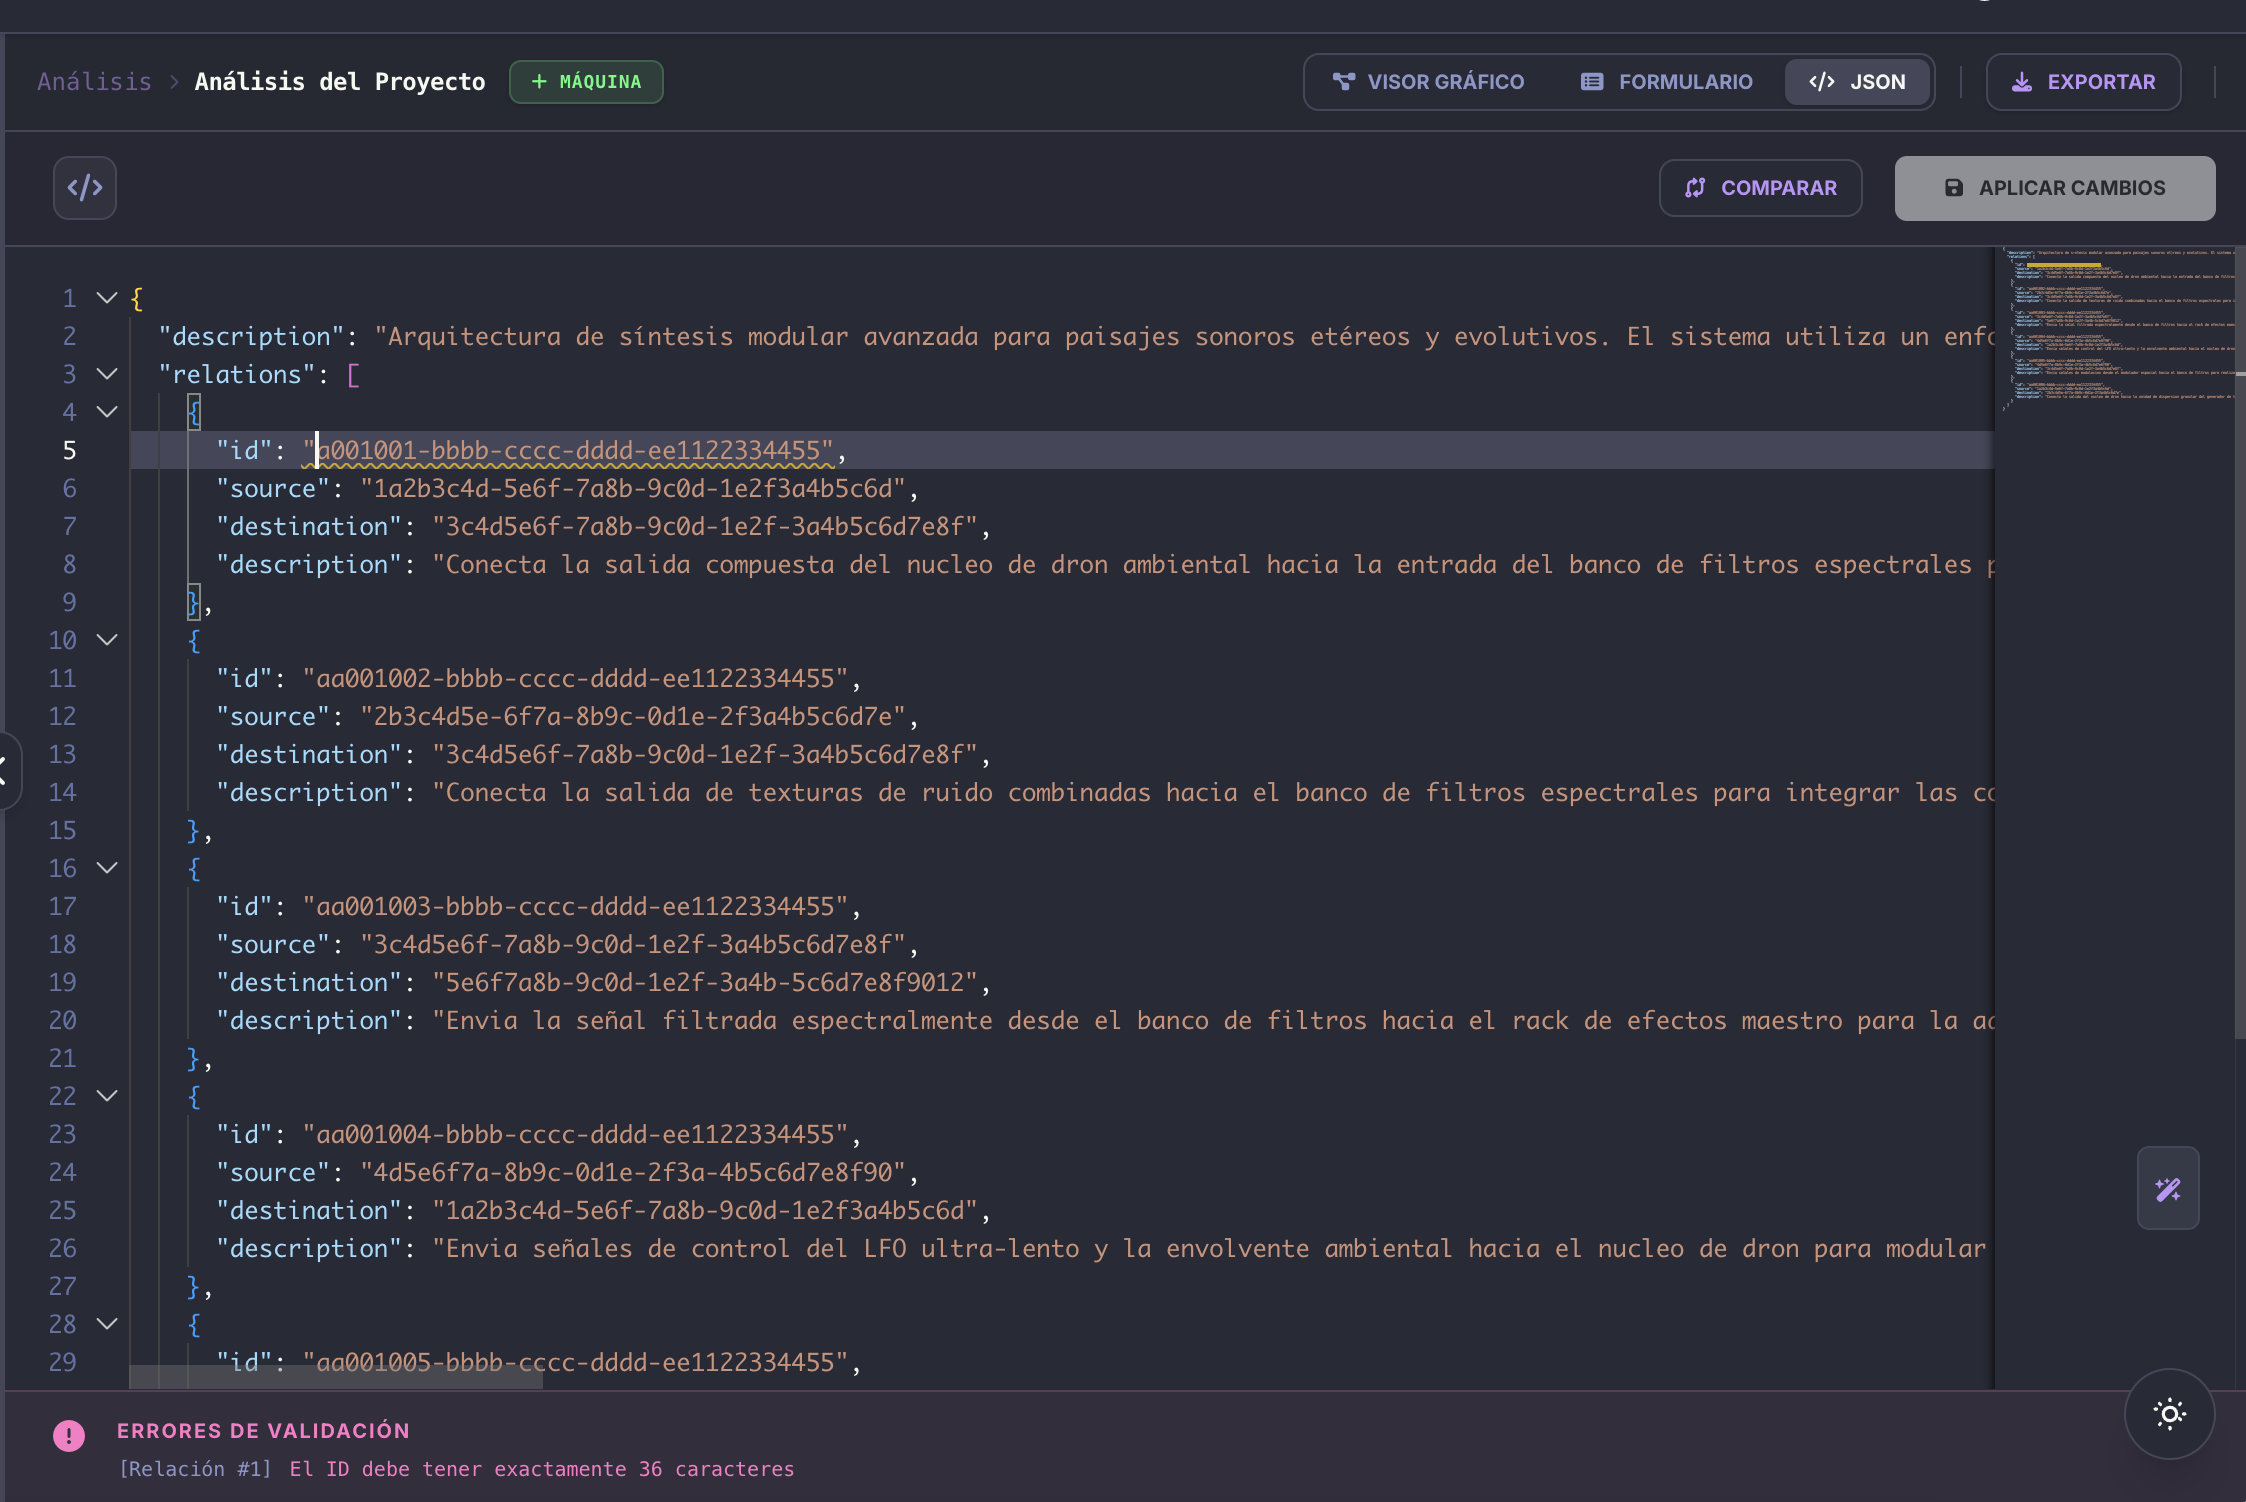
\includegraphics[width=\textwidth]{imagenes/05_analisis/12_gestionErroresEditorJsonRelacionesCim.png}
    \caption{Sistema de validación en tiempo real en el editor JSON.}
\end{figure}

El sistema verifica la estructura de forma continua. Ante un defecto sintáctico o un incumplimiento del modelo de dominio, el editor señala el error explícitamente, bloqueando el guardado de modelos inconsistentes.

\begin{figure}[!ht]
    \centering
    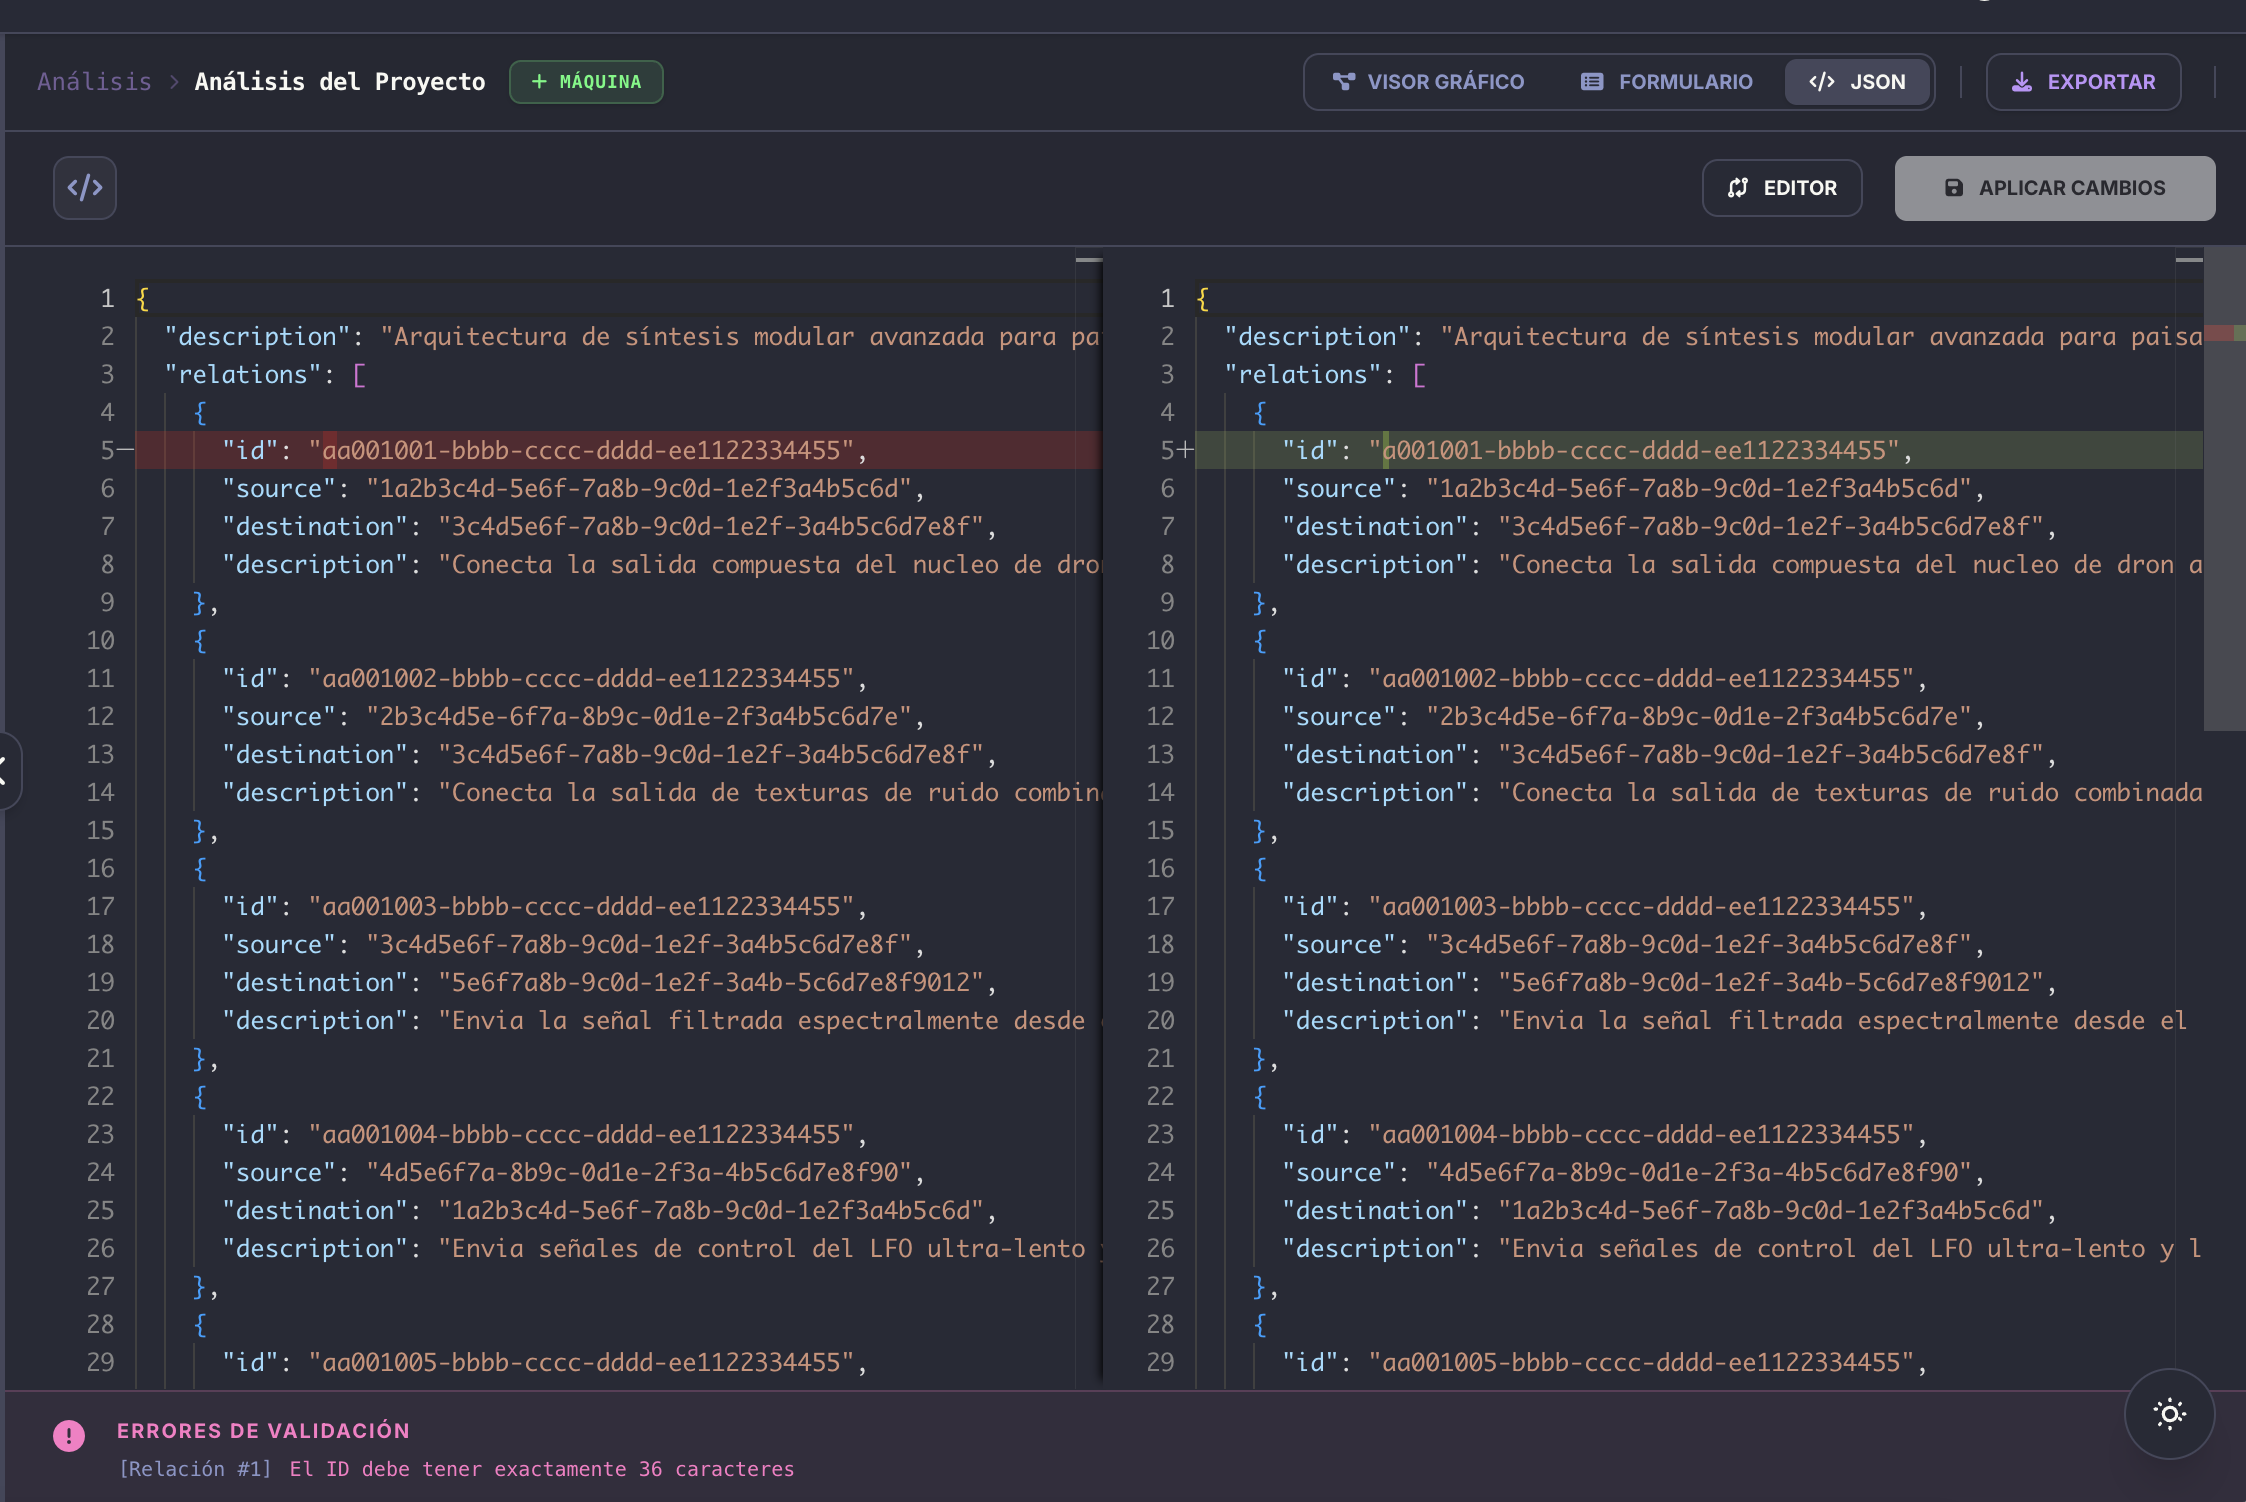
\includegraphics[width=\textwidth]{imagenes/05_analisis/13_comparadorEditorJsonRelacionesCim.png}
    \caption{Herramienta visual de diferencias (Diff) en el editor JSON.}
\end{figure}

Para gestionar cambios complejos, la herramienta de \textit{diff} permite comparar las alteraciones en curso con la última versión guardada, garantizando un control de versiones a nivel de sesión.

\begin{figure}[!ht]
    \centering
    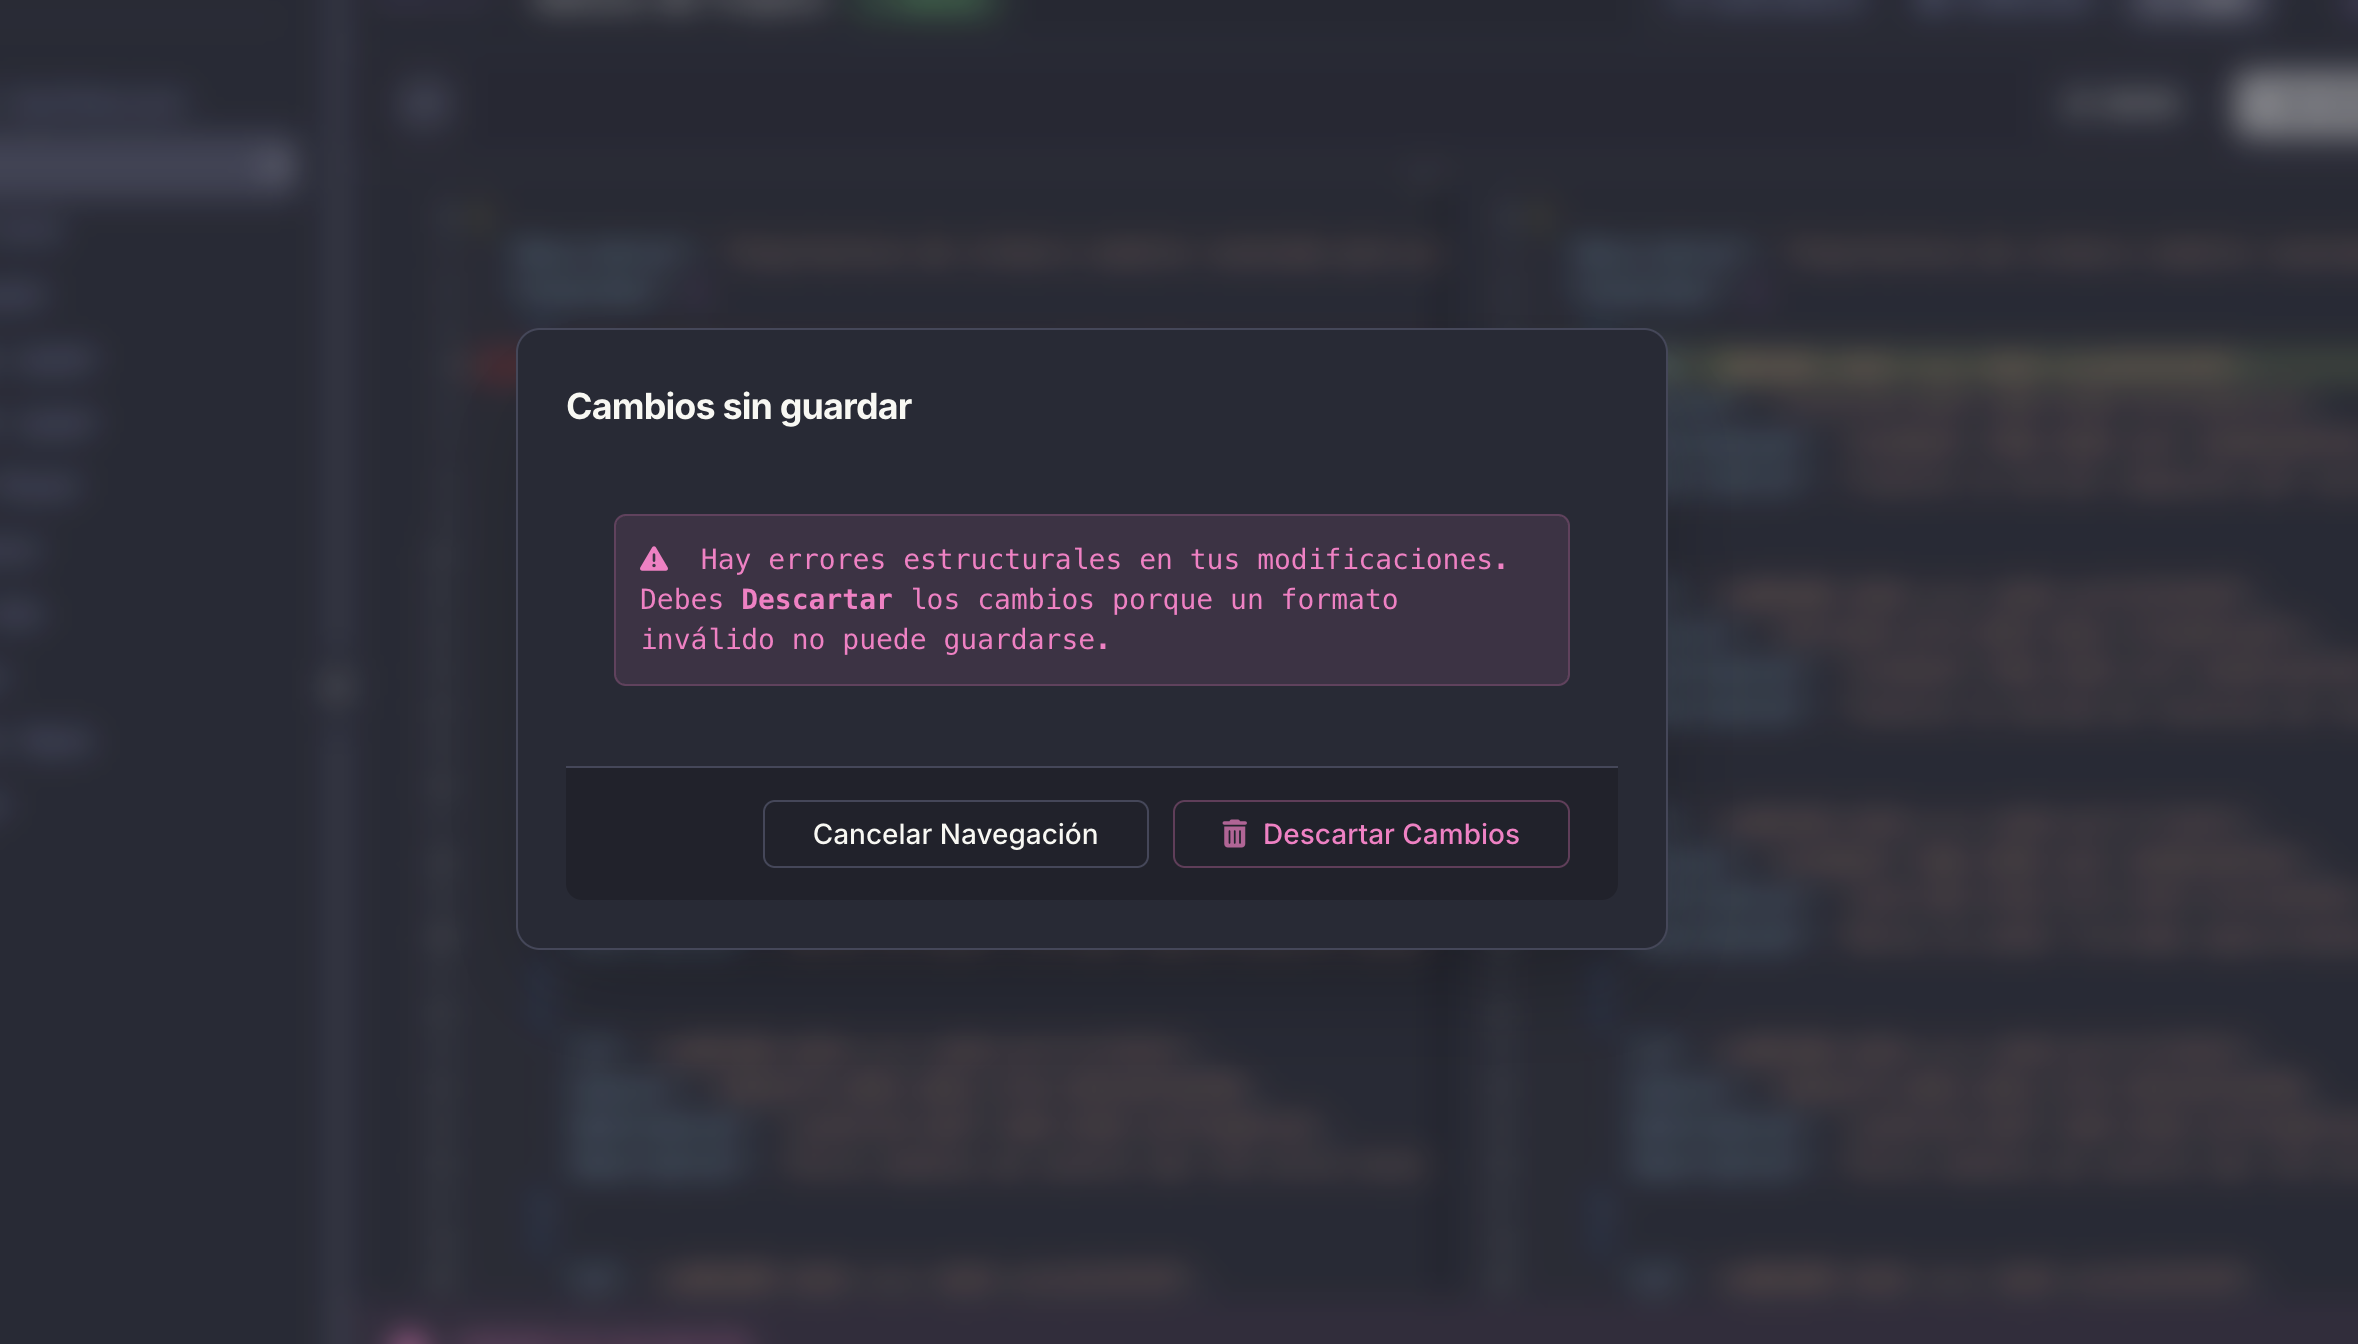
\includegraphics[width=0.6\textwidth]{imagenes/05_analisis/15_cambiarDePantallaSinGuardarJsonRelacionesCim.png}
    \caption{Aviso preventivo por cambios no guardados.}
\end{figure}

\begin{figure}[!ht]
    \centering
    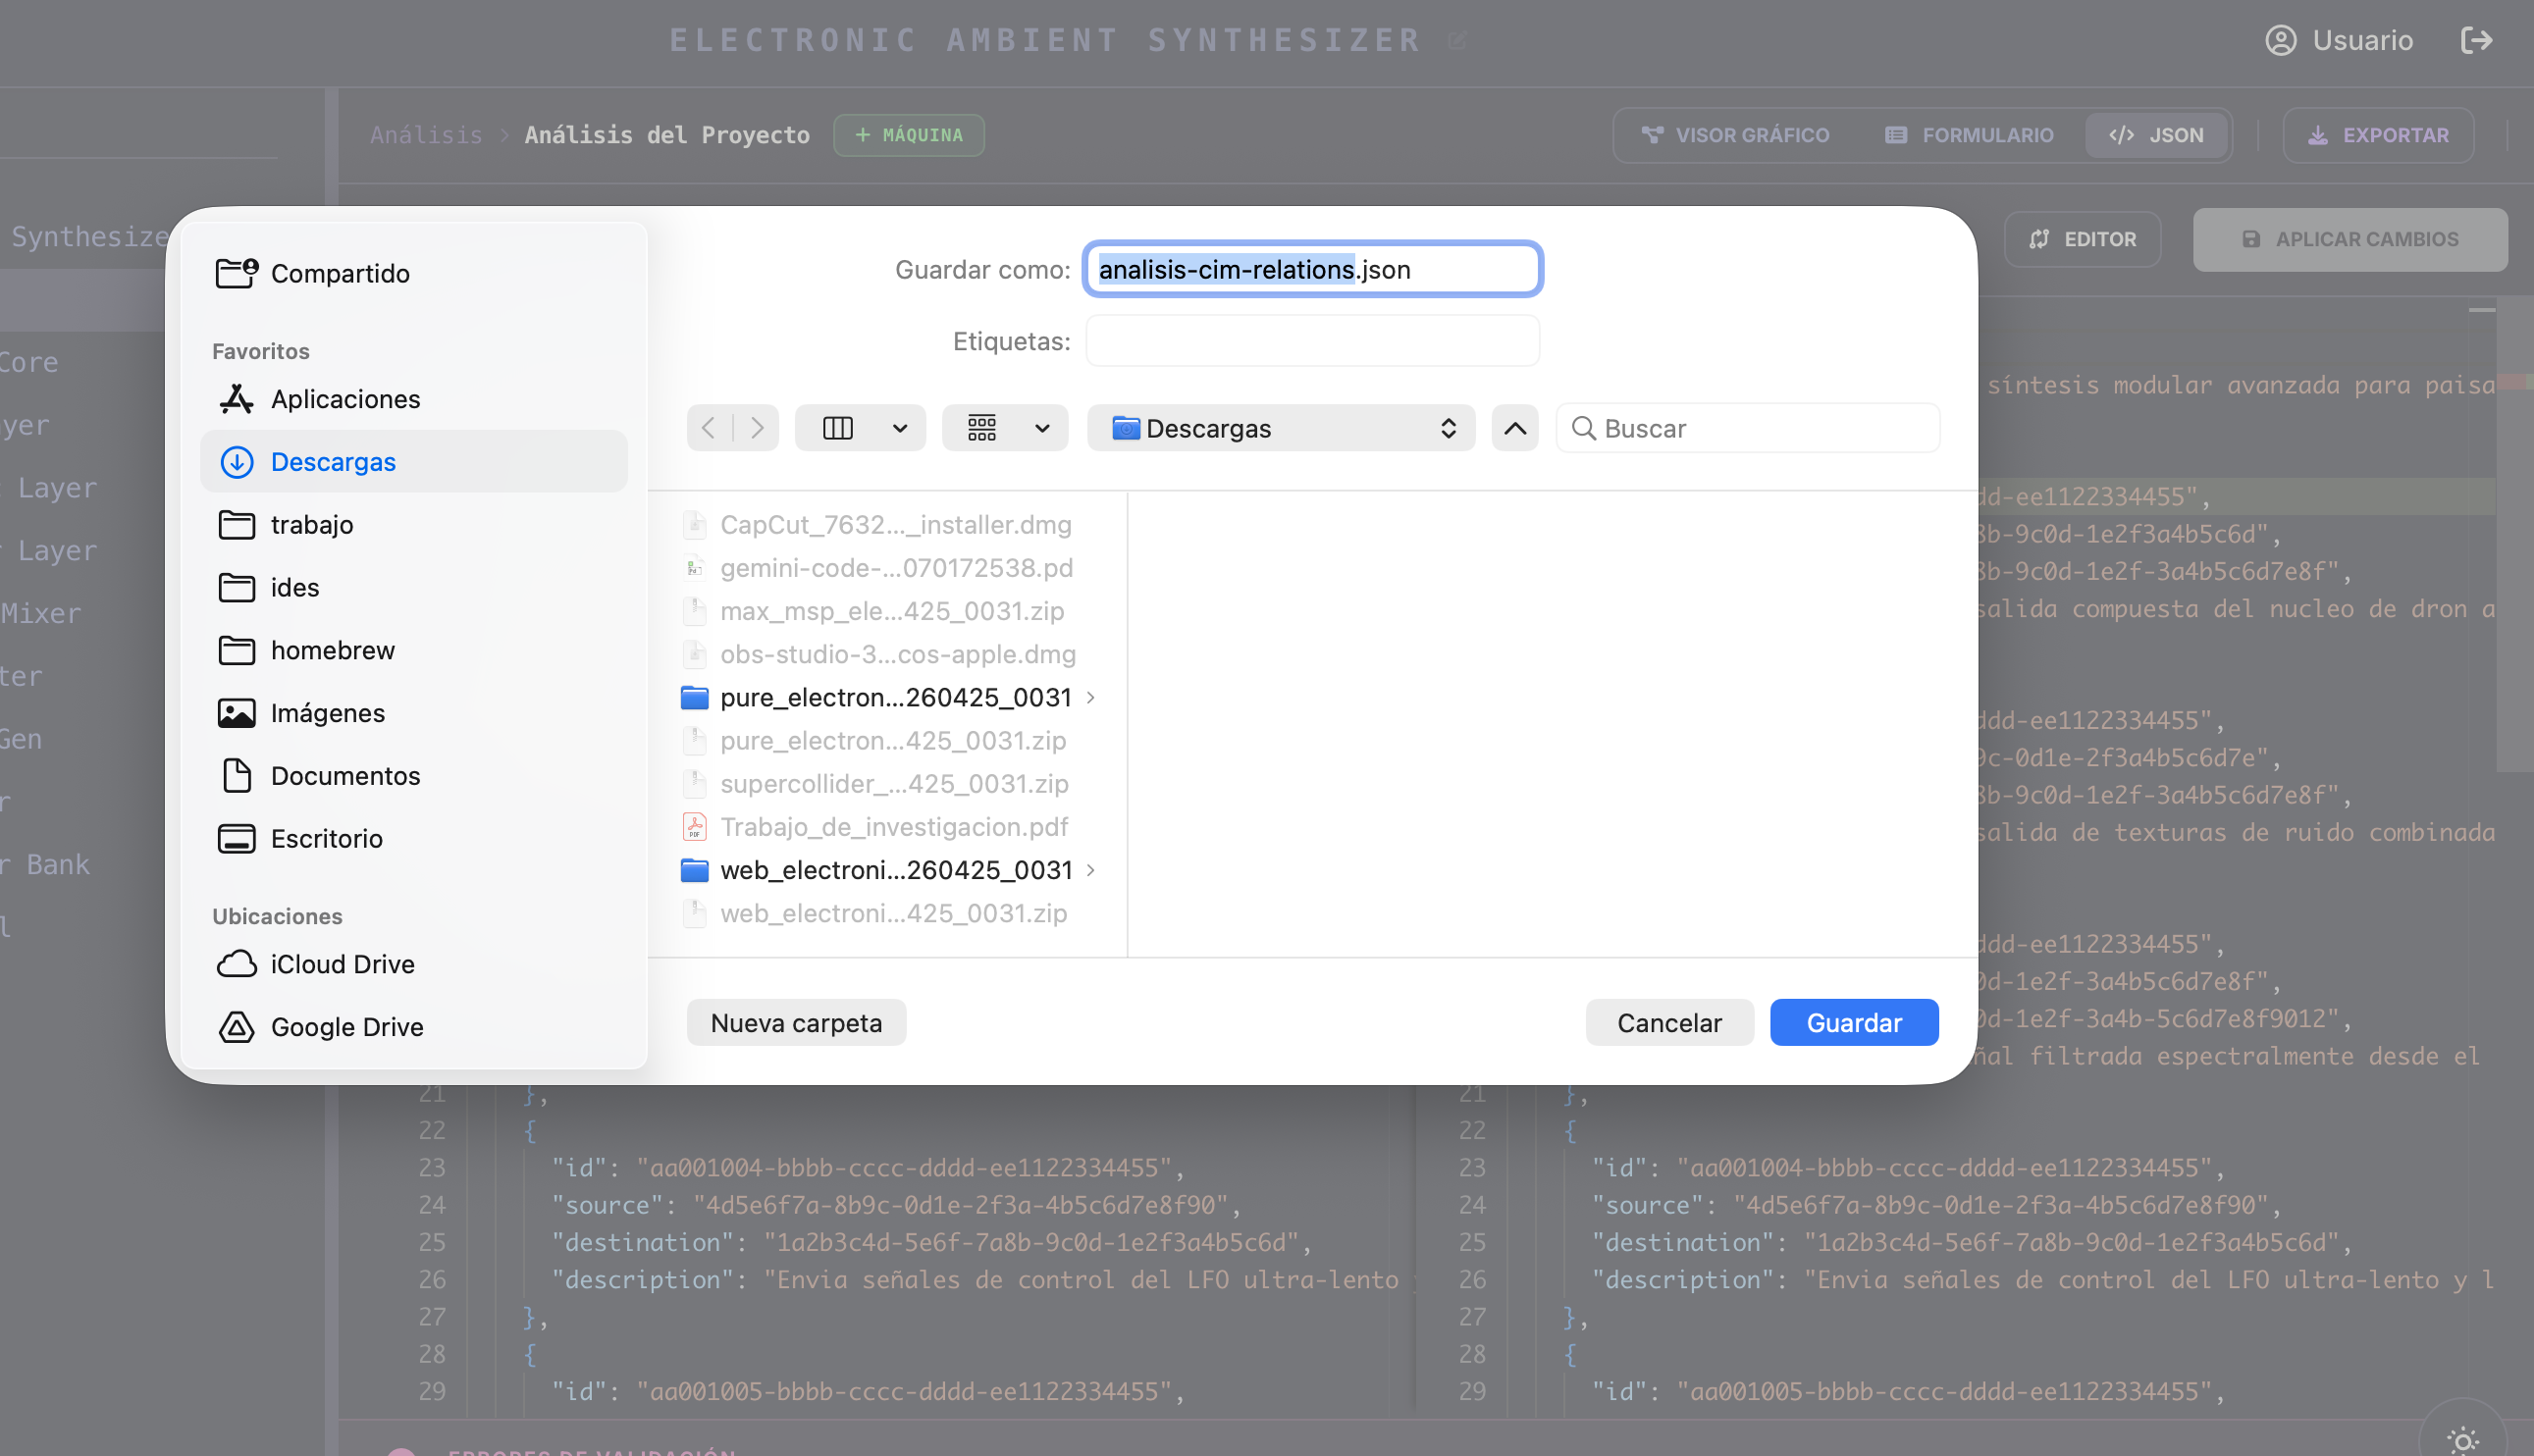
\includegraphics[width=0.6\textwidth]{imagenes/05_analisis/14_exportacionJsonRelacionesCim.png}
    \caption{Opciones de exportación del modelo de relaciones.}
\end{figure}

El entorno cuenta con barreras de seguridad, advirtiendo al usuario si intenta cambiar de vista sin guardar. Asimismo, incluye capacidades de exportación para guardar localmente el modelo \textit{JSON} consolidado.

\section{Edición de Máquinas CIM Internas}

Una vez definida la red general, cada máquina conceptual requiere la configuración pormenorizada de su lógica interna y componentes de interfaz.

\begin{figure}[!ht]
    \centering
    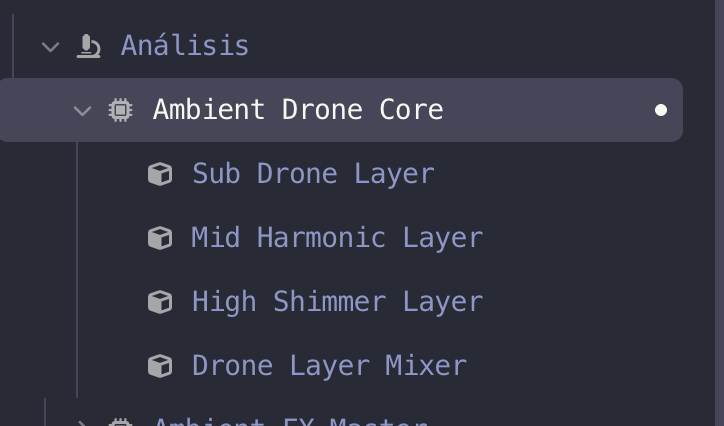
\includegraphics[width=0.4\textwidth]{imagenes/05_analisis/16_maquinaCimEnExplorador.png}
    \caption{Acceso a la configuración específica de una máquina CIM en el explorador.}
\end{figure}

Al seleccionar una máquina concreta en el árbol del explorador, se abre un panel focalizado en su arquitectura interna.

\begin{figure}[!ht]
    \centering
    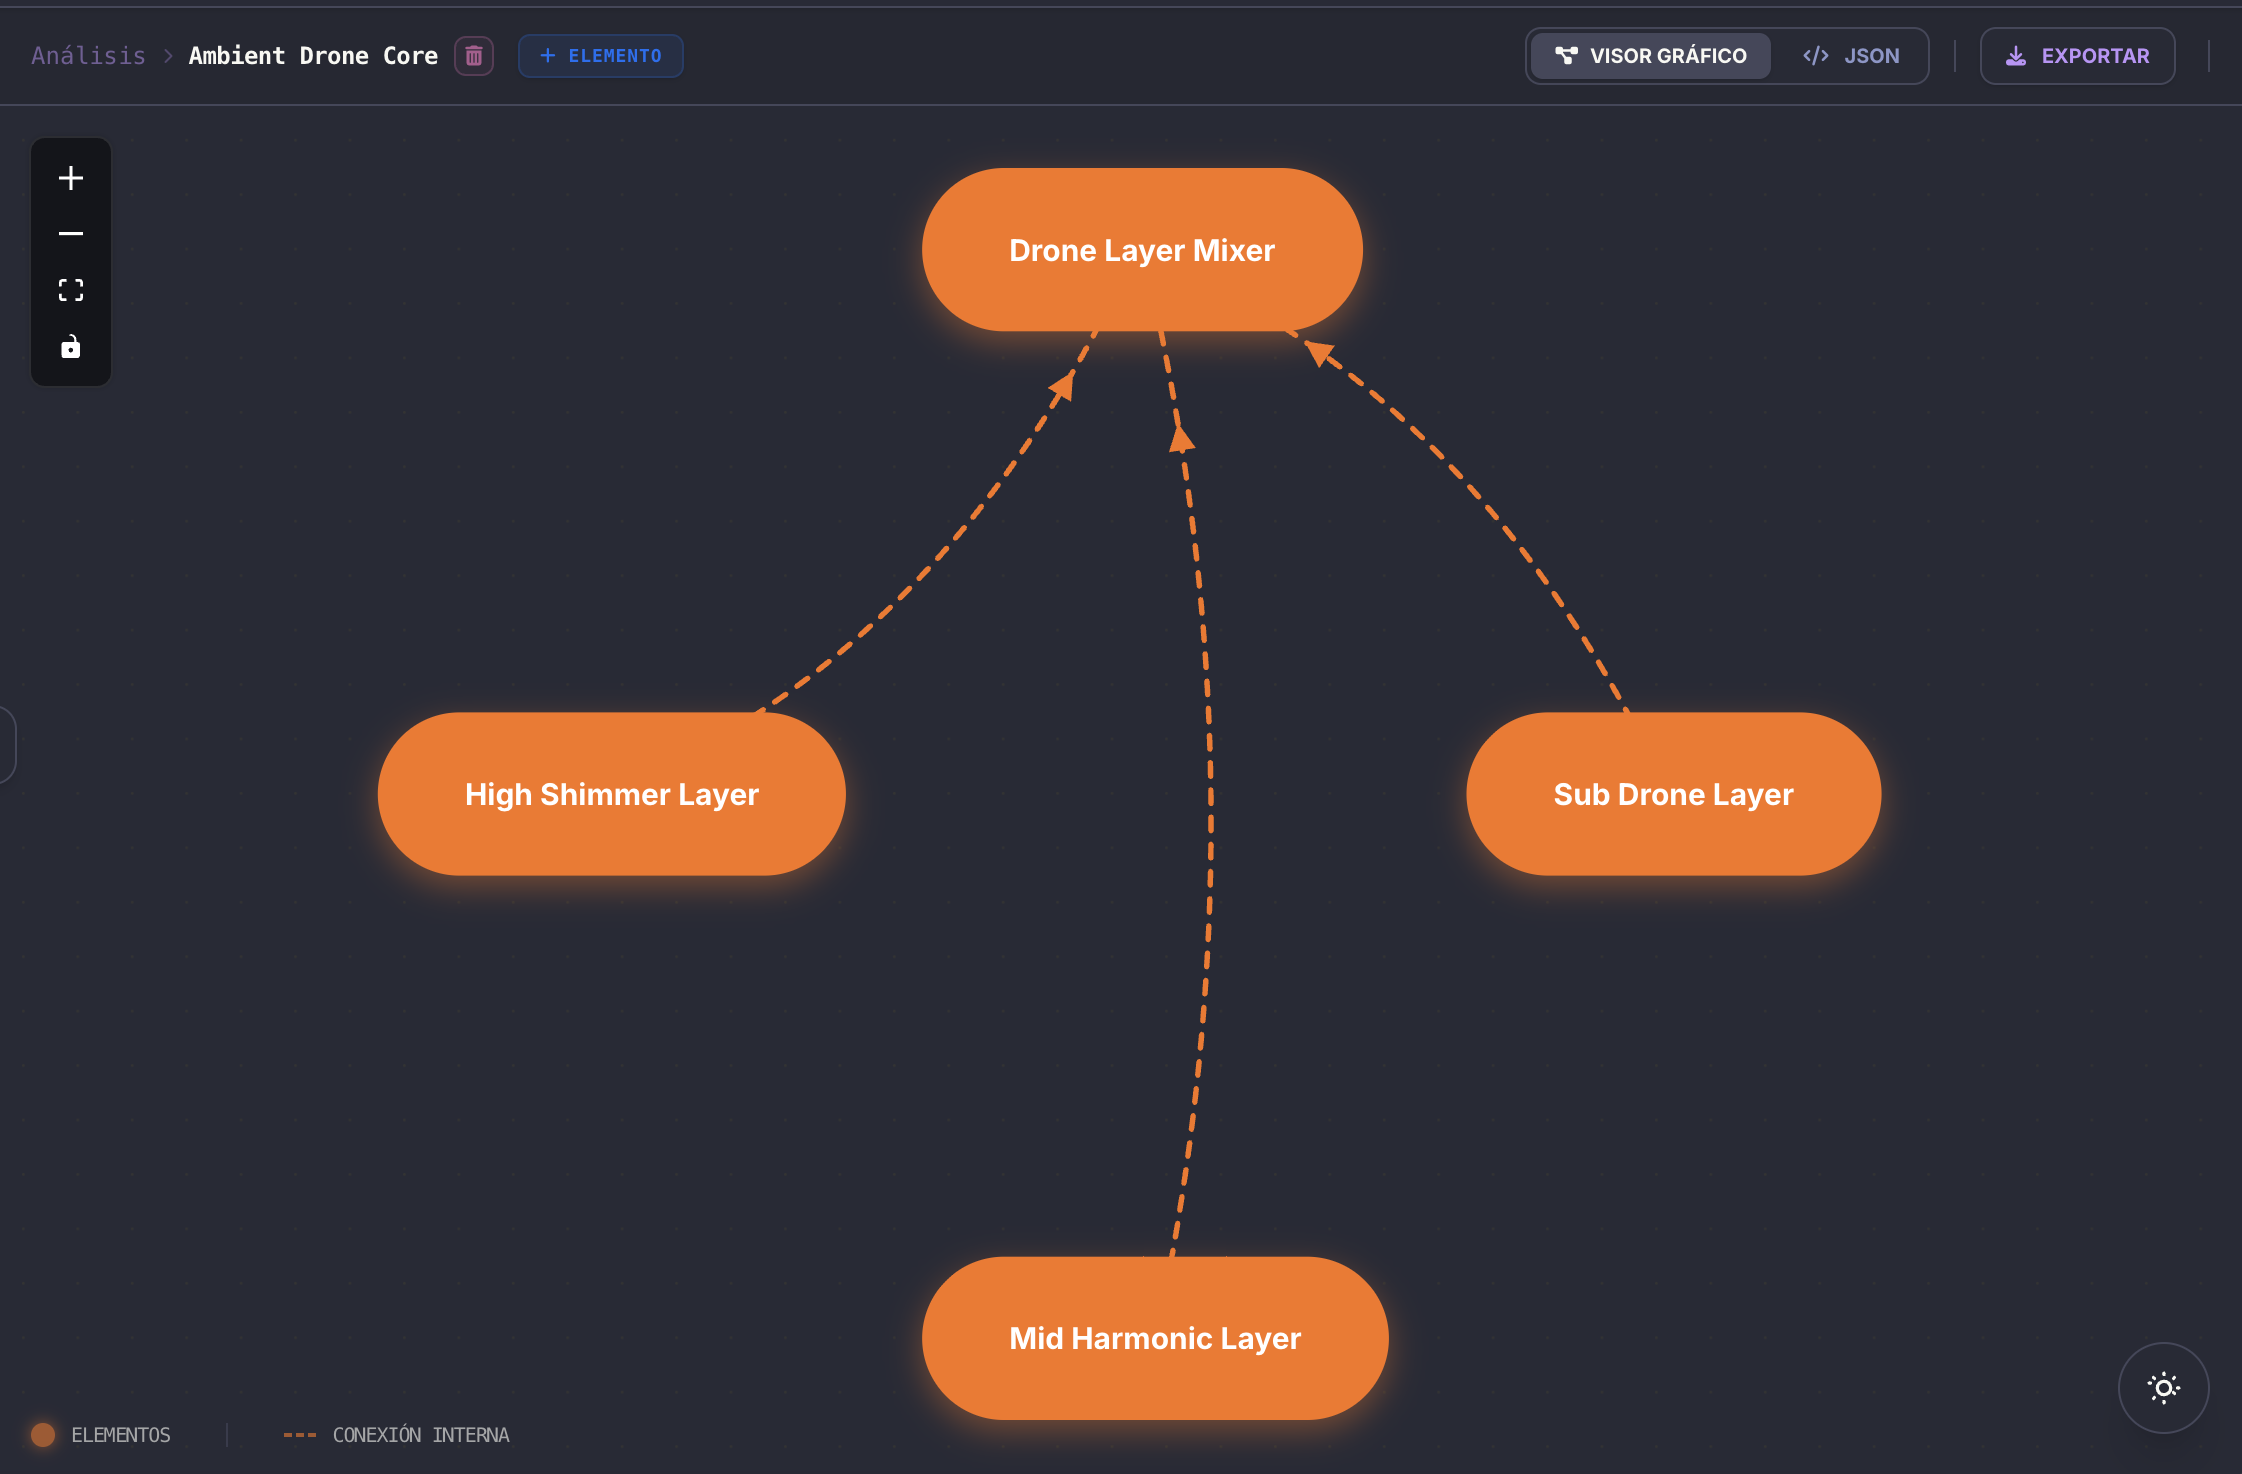
\includegraphics[width=\textwidth]{imagenes/05_analisis/17_visorGraficoMaquinaCim.png}
    \caption{Visor gráfico de la estructura interna de la máquina CIM.}
\end{figure}

\begin{figure}[!ht]
    \centering
    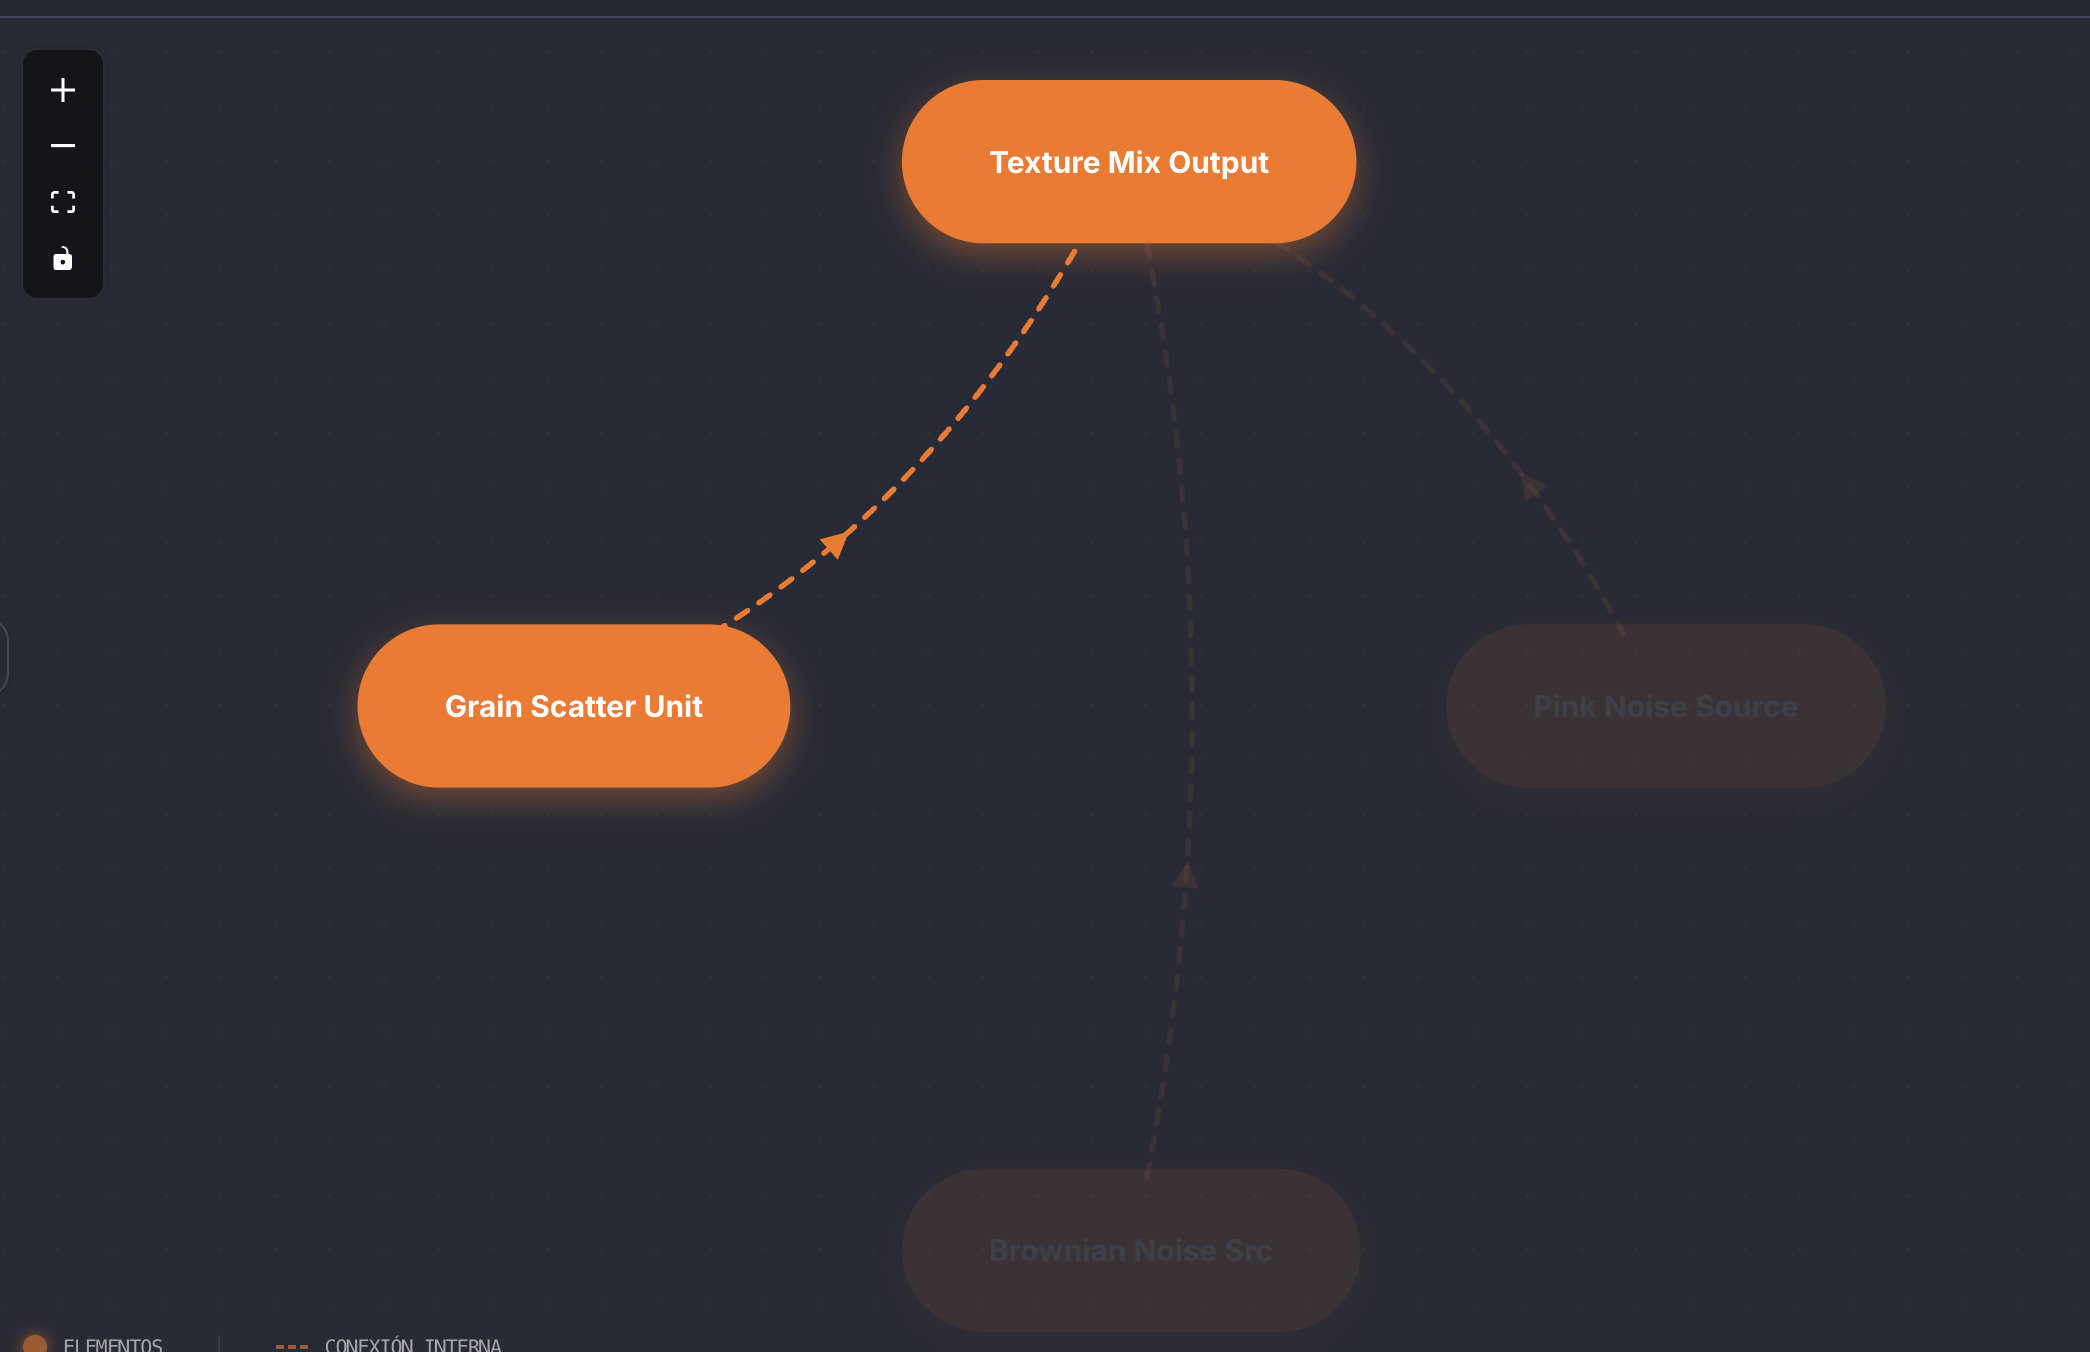
\includegraphics[width=\textwidth]{imagenes/05_analisis/18_visorGraficoMaquinaCimAristaPulsada.png}
    \caption{Inspección de las conexiones lógicas internas.}
\end{figure}

\begin{figure}[!ht]
    \centering
    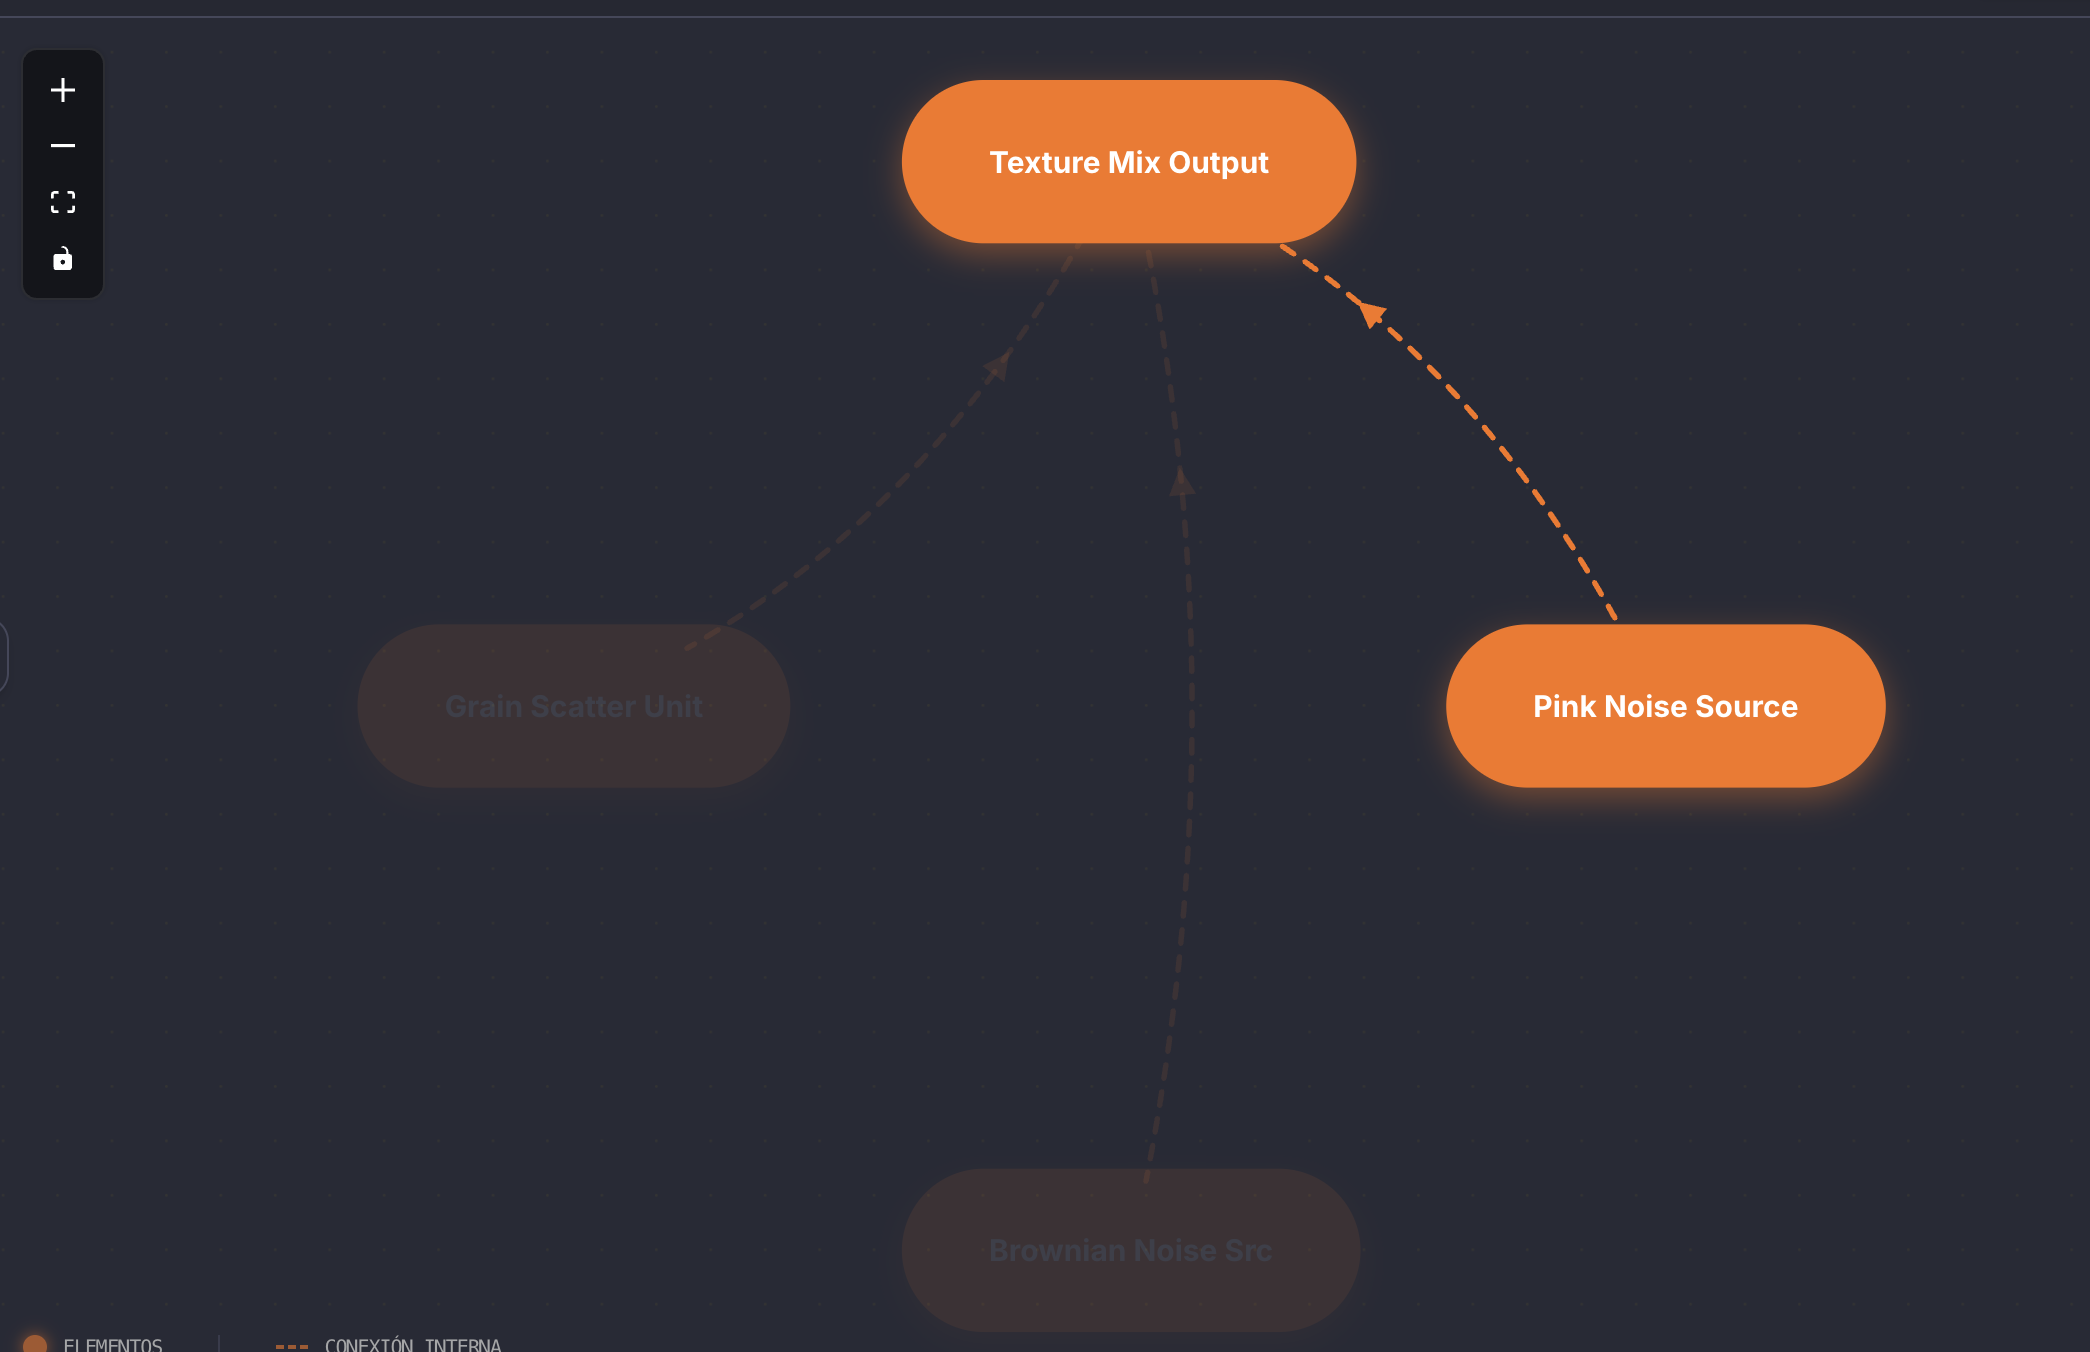
\includegraphics[width=\textwidth]{imagenes/05_analisis/19_visorGraficoMaquinaCimNodoPulsado.png}
    \caption{Inspección de las propiedades de los puertos y parámetros internos.}
\end{figure}

Al igual que en el nivel superior, existe un visor interactivo que mapea los bloques funcionales, puertos y conexiones internas que dotan de comportamiento al elemento musical conceptual.

\subsection{Gestión de Elementos de Máquina}

\begin{figure}[!ht]
    \centering
    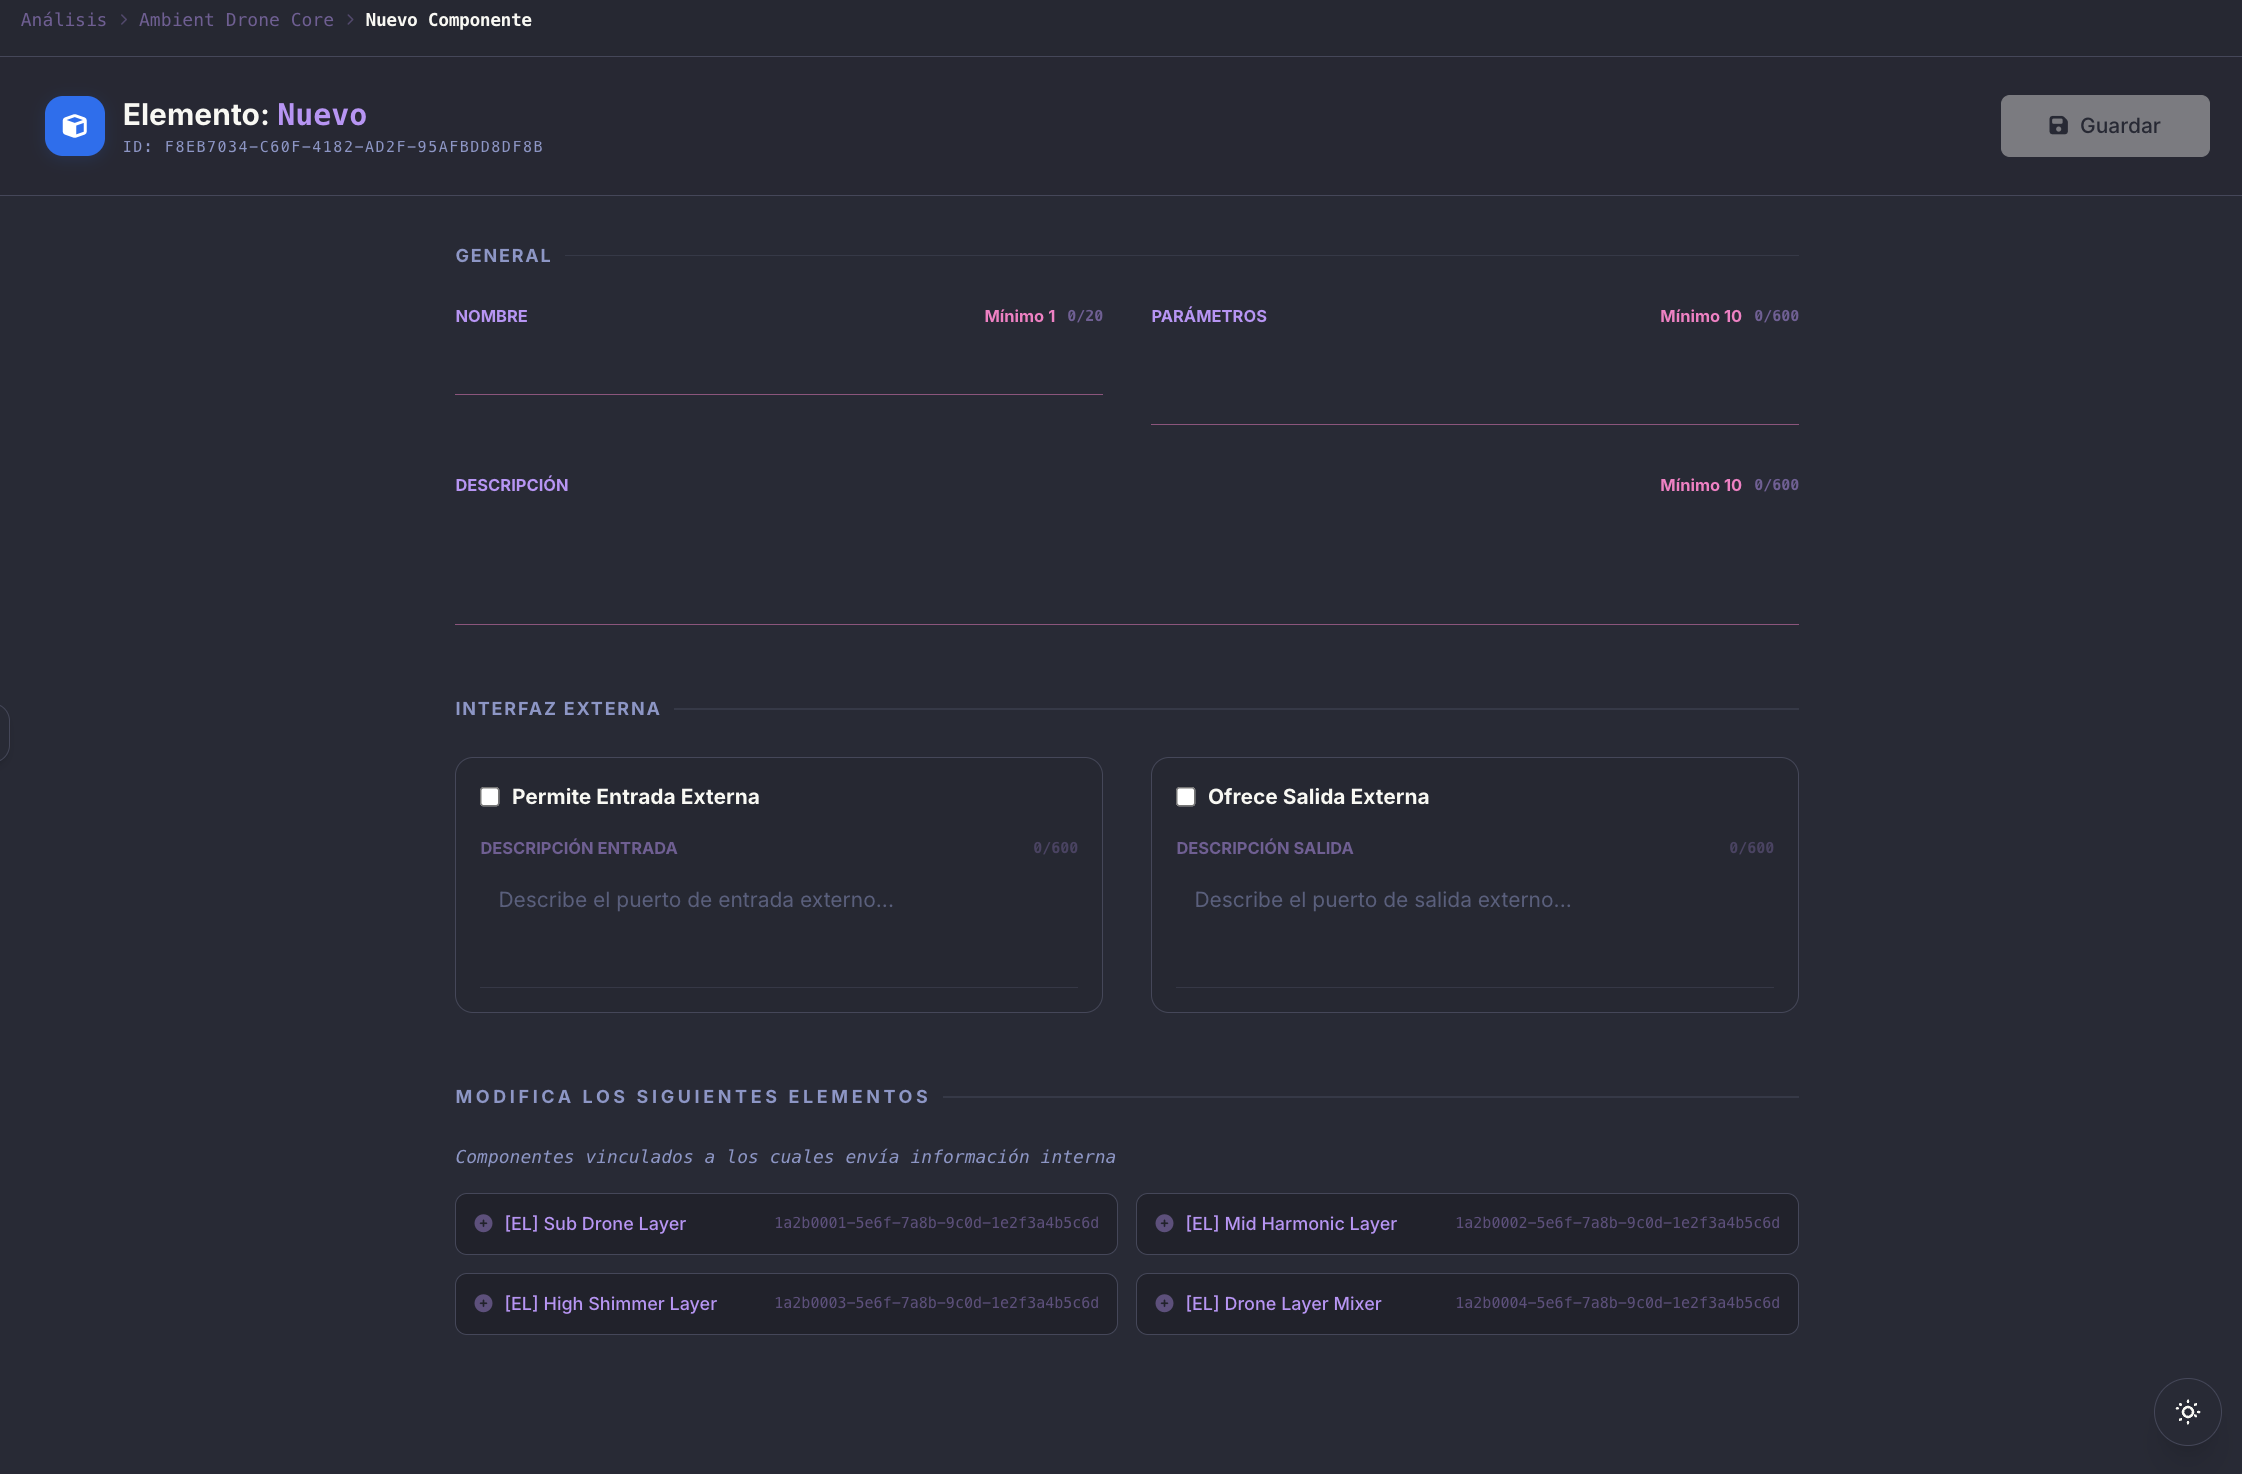
\includegraphics[width=\textwidth]{imagenes/05_analisis/20_formularioCrearElementoDeMaquinaCim.png}
    \caption{Formulario para la adición de nuevos elementos internos.}
\end{figure}

\begin{figure}[!ht]
    \centering
    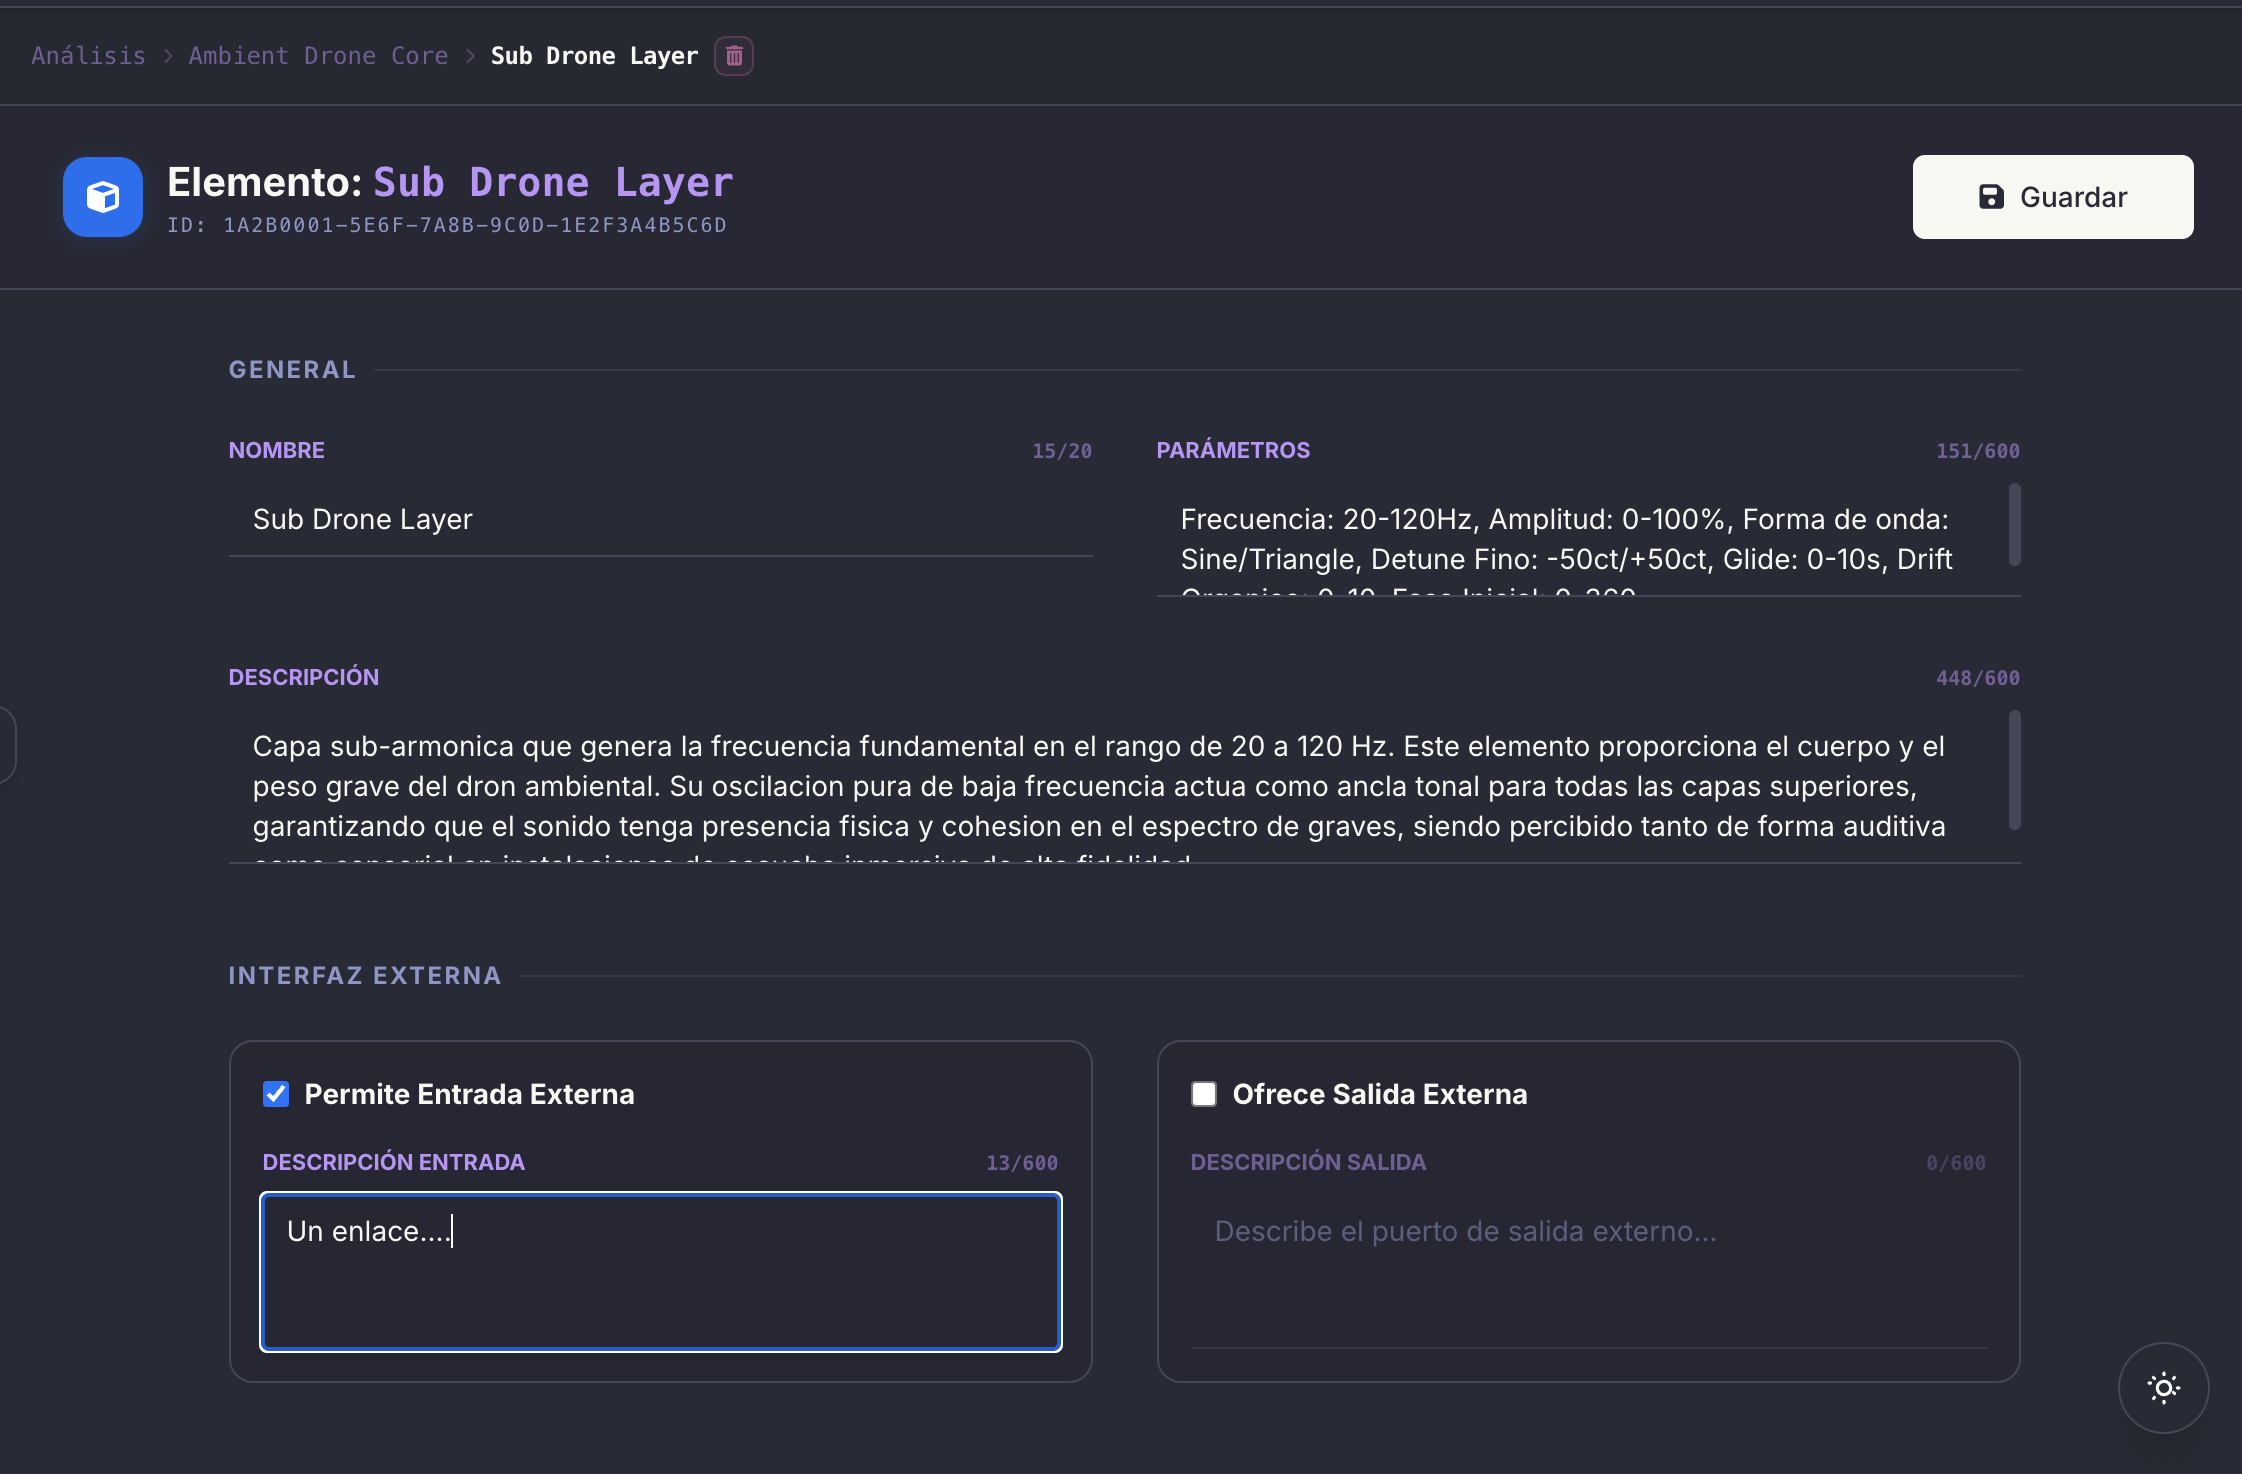
\includegraphics[width=\textwidth]{imagenes/05_analisis/21_formularioRellenoElementoMaquinaCim.png}
    \caption{Vista detallada de un elemento interno con su configuración completa.}
\end{figure}

El formulario de edición de elementos asiste en la asignación de atributos vitales (tipos, dominios, valores predeterminados) definidos por el modelo de datos \textit{CIM}.

\begin{figure}[!ht]
    \centering
    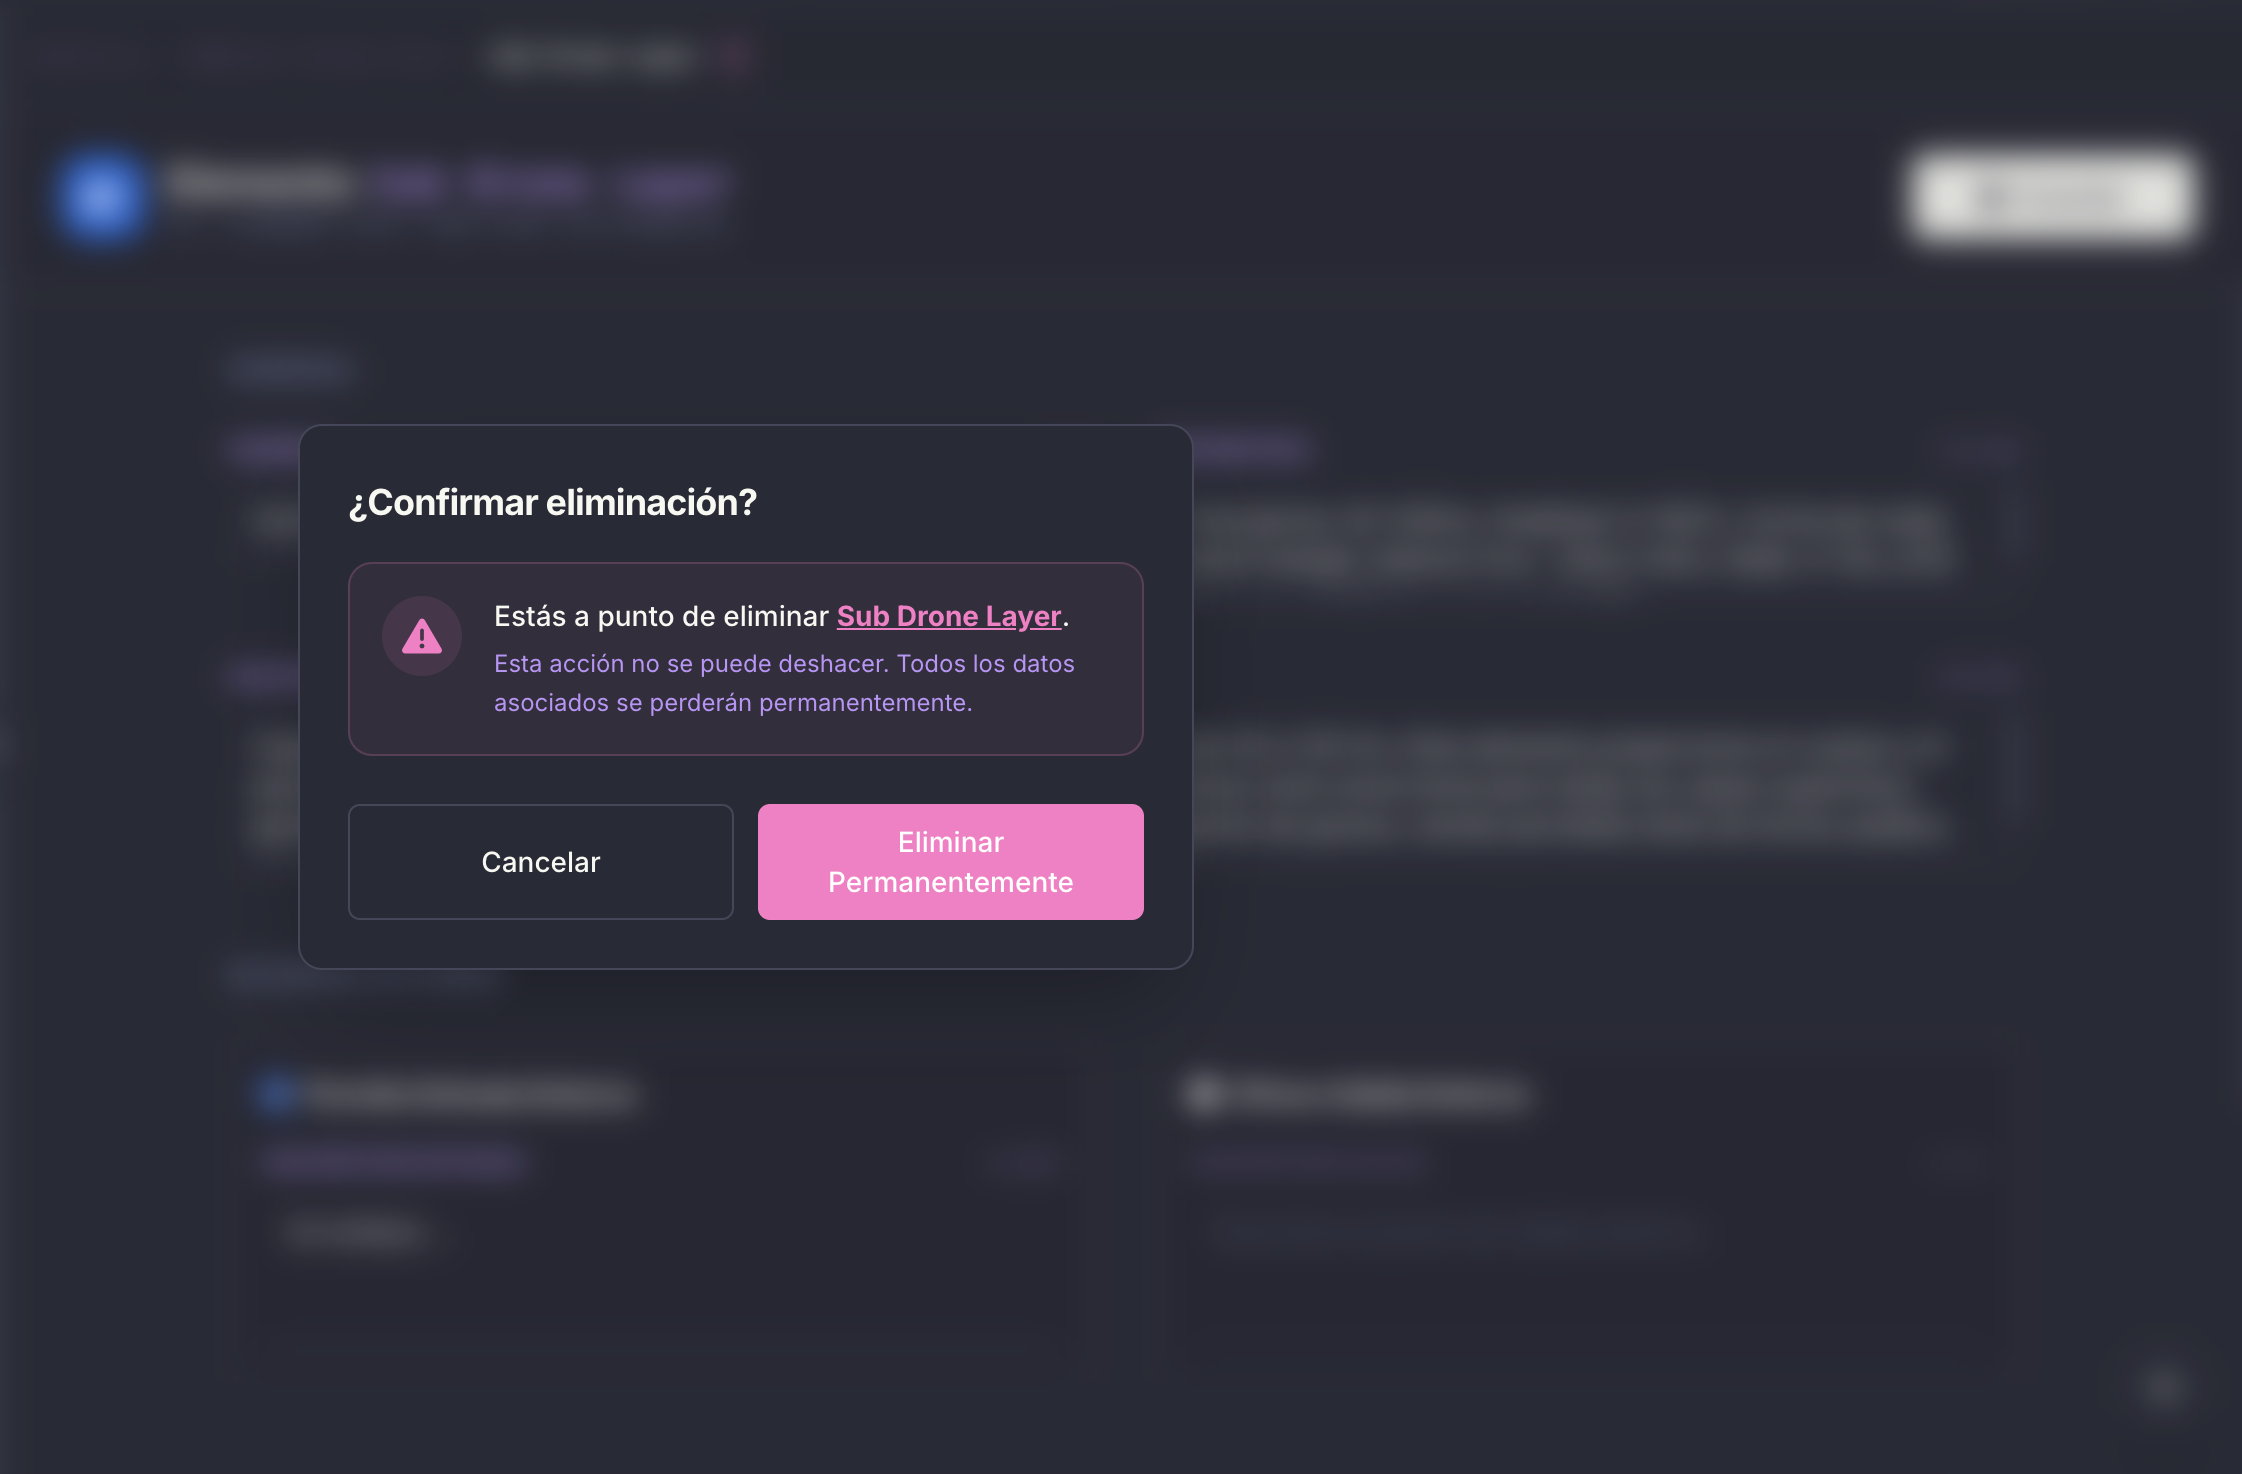
\includegraphics[width=0.6\textwidth]{imagenes/05_analisis/22_eliminarElementoMaquinaCim.png}
    \caption{Solicitud de confirmación para eliminar un componente interno.}
\end{figure}

\begin{figure}[!ht]
    \centering
    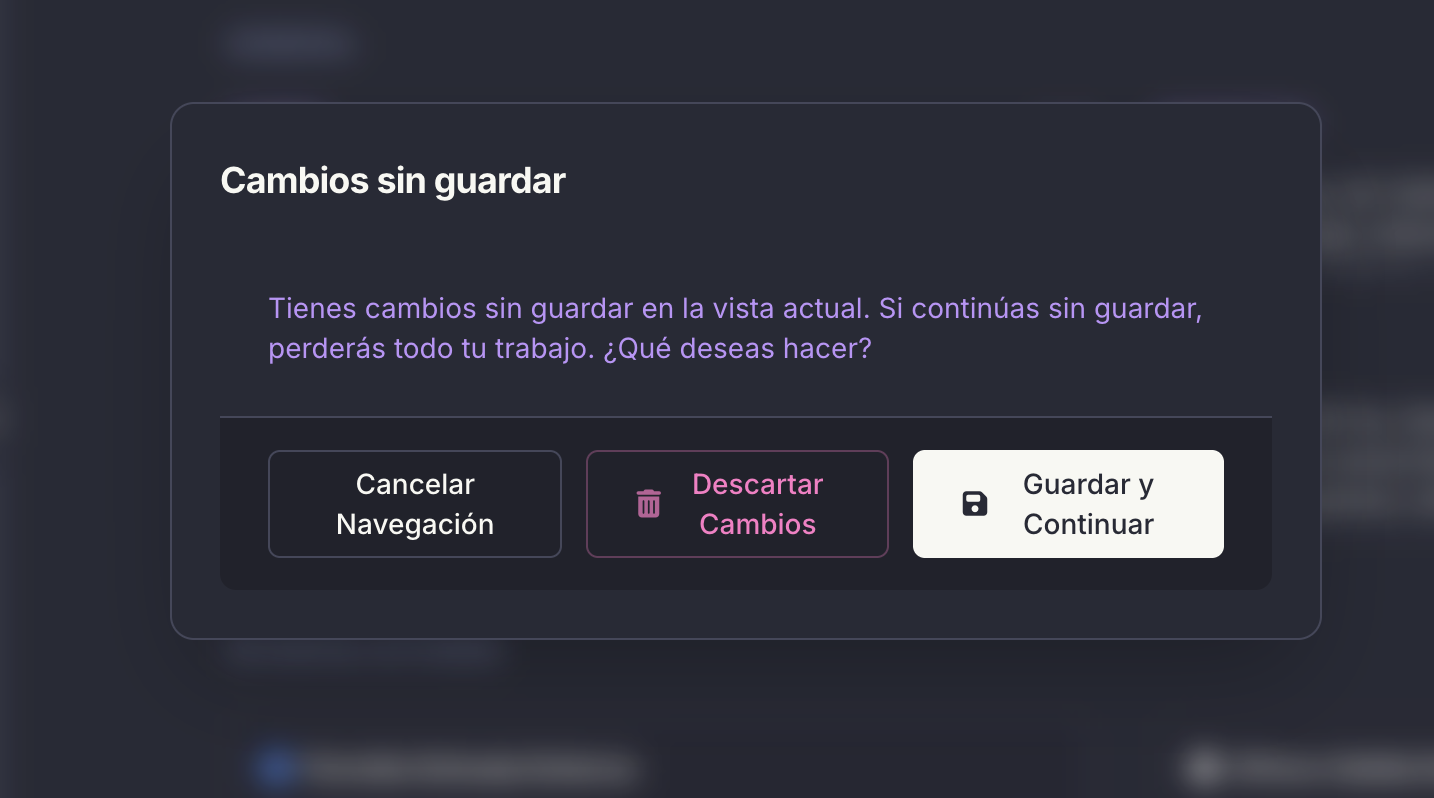
\includegraphics[width=0.6\textwidth]{imagenes/05_analisis/23_salirDeFromularioElemengtoMaquinaCimSinSalvar.png}
    \caption{Protección contra pérdida de datos al editar elementos de máquina.}
\end{figure}

La modificación de los interiores de la máquina está protegida mediante validaciones y cuadros de diálogo de confirmación, asegurando que las alteraciones estructurales (eliminaciones o abandonos no guardados) sean siempre acciones deliberadas del usuario.

\chapter{Diseño Conceptual (PIM)}

\section{El Modelo Independiente de Plataforma}

El Diseño Conceptual representa la fase de traducción y especialización técnica dentro del flujo \textit{MDAA}. En esta etapa, el usuario elabora el \textit{PIM} (\textit{Platform Independent Model}), donde los requerimientos puramente musicales del \textit{CIM} se enriquecen con conceptos computacionales y arquitectónicos, aunque manteniéndose independientes de la tecnología final de despliegue.

\begin{figure}[!ht]
    \centering
    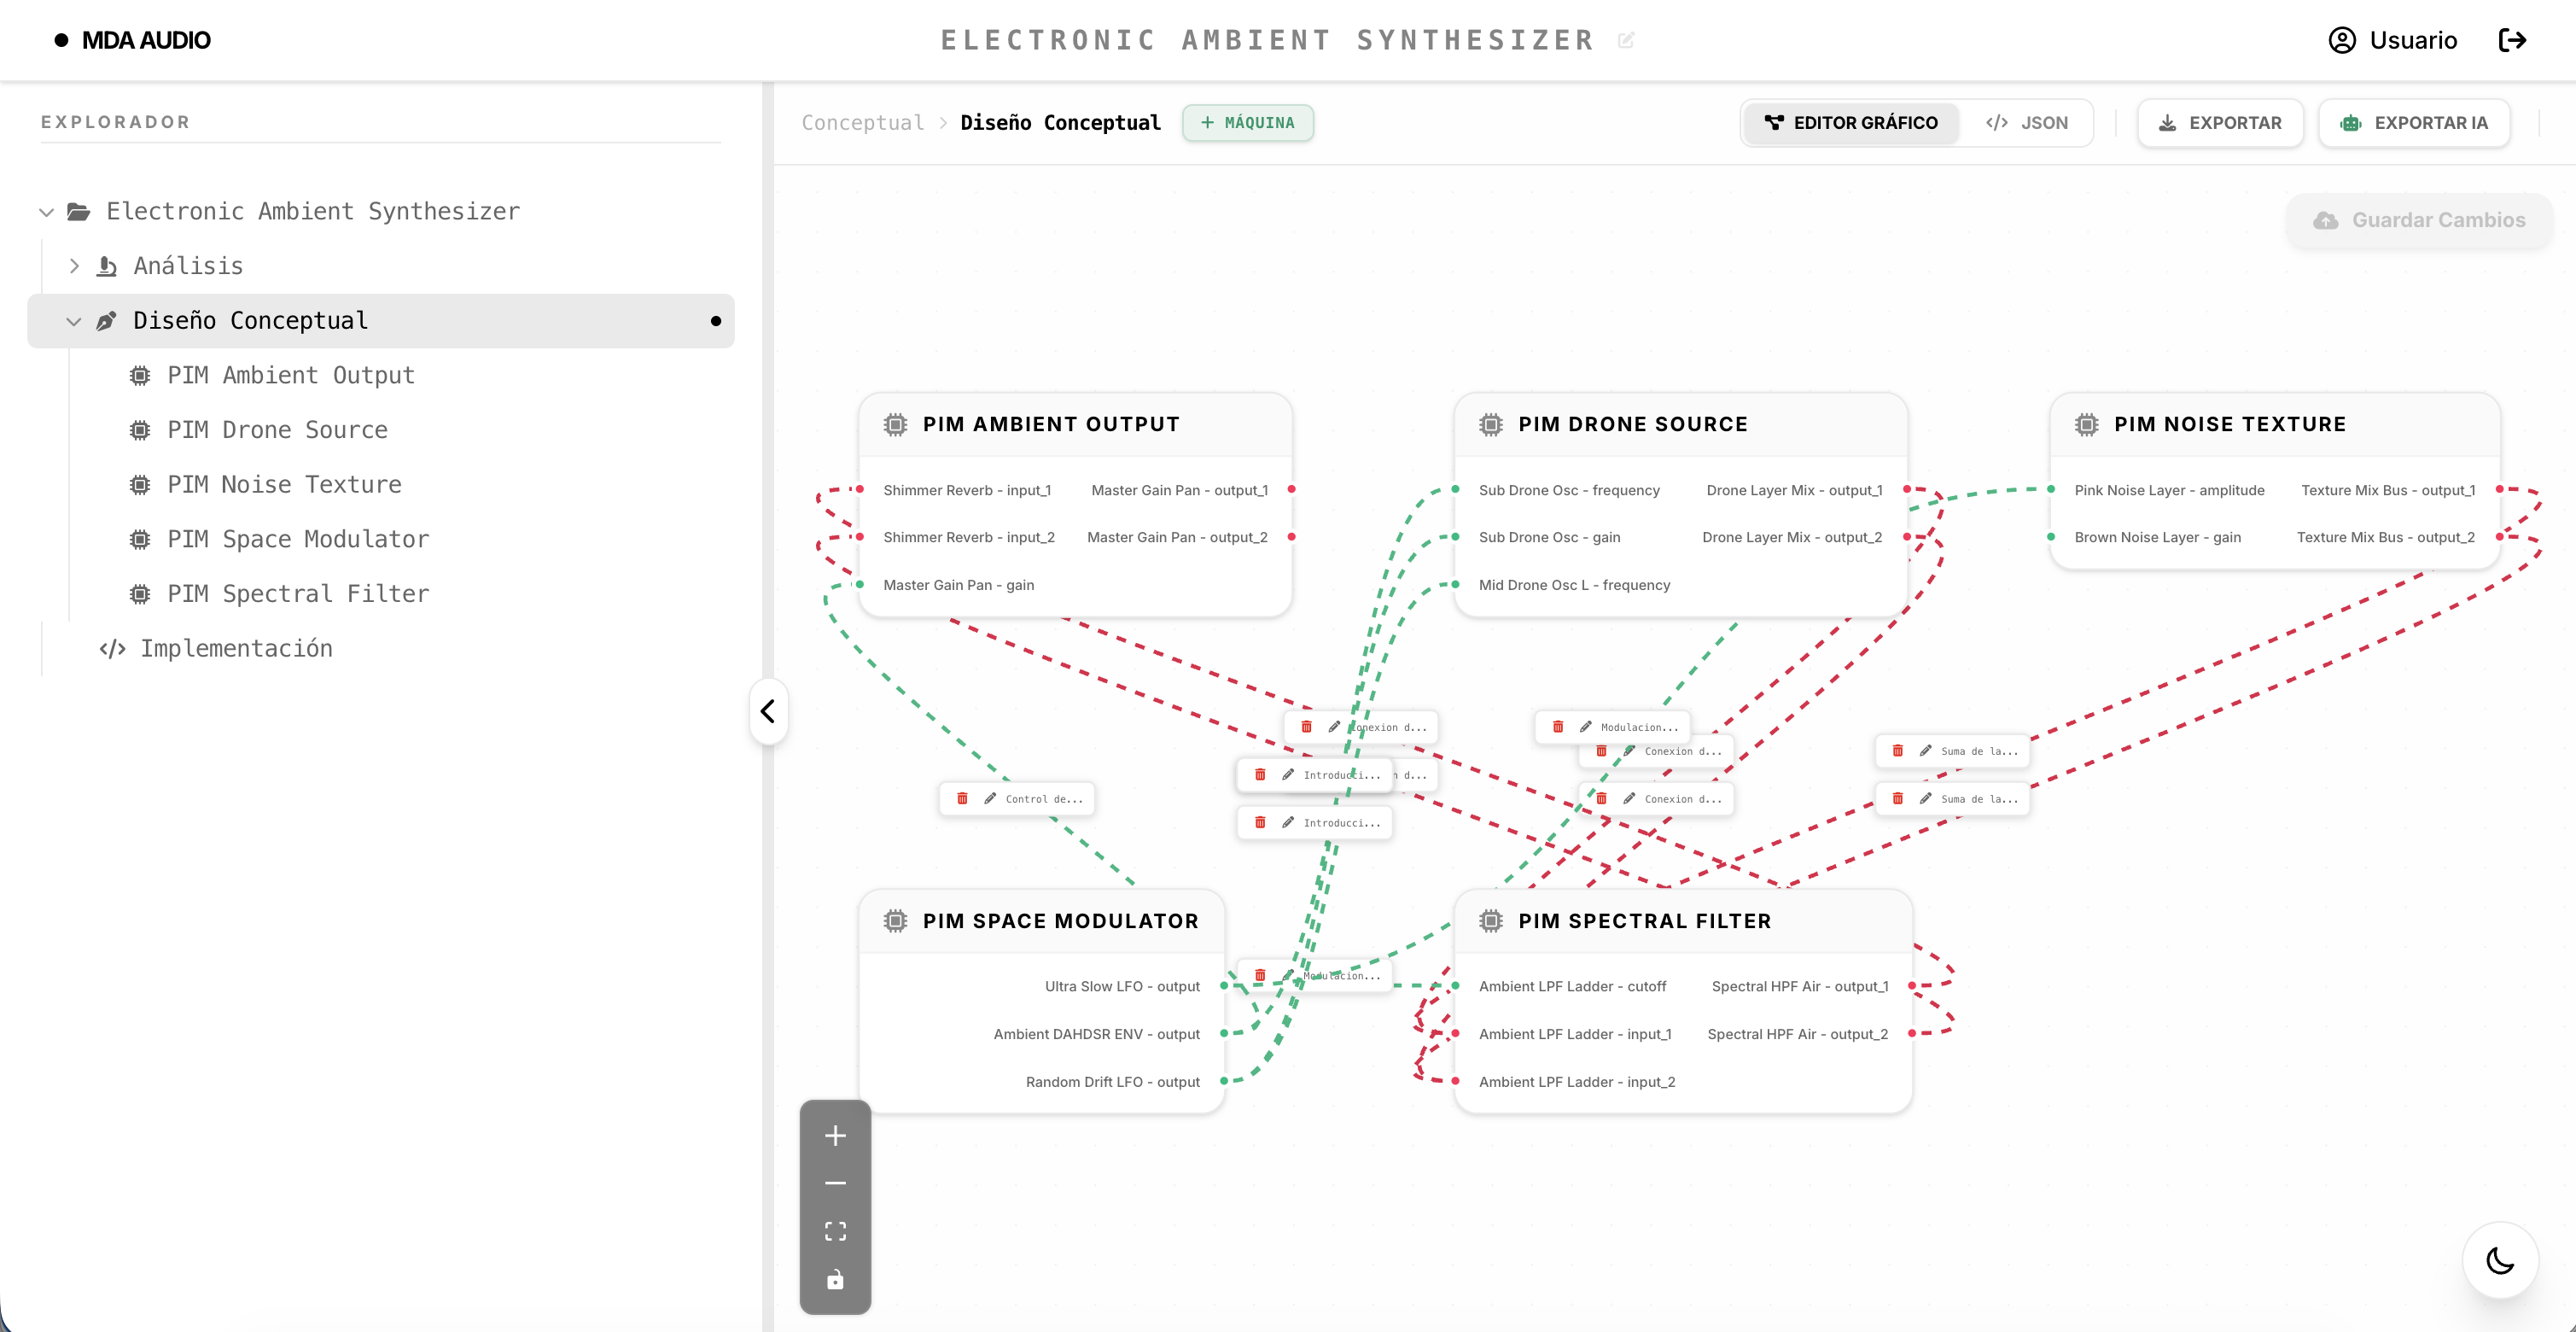
\includegraphics[width=\textwidth]{imagenes/06_diseno/01_pantallaDisenoConceptual.png}
    \caption{Vista general del entorno de Diseño Conceptual.}
\end{figure}

Al navegar a la sección de Diseño Conceptual, la aplicación presenta herramientas destinadas a vincular y mapear las construcciones teóricas hacia estructuras de diseño de software (ej. componentes, bloques de procesamiento de audio).

\begin{figure}[!ht]
    \centering
    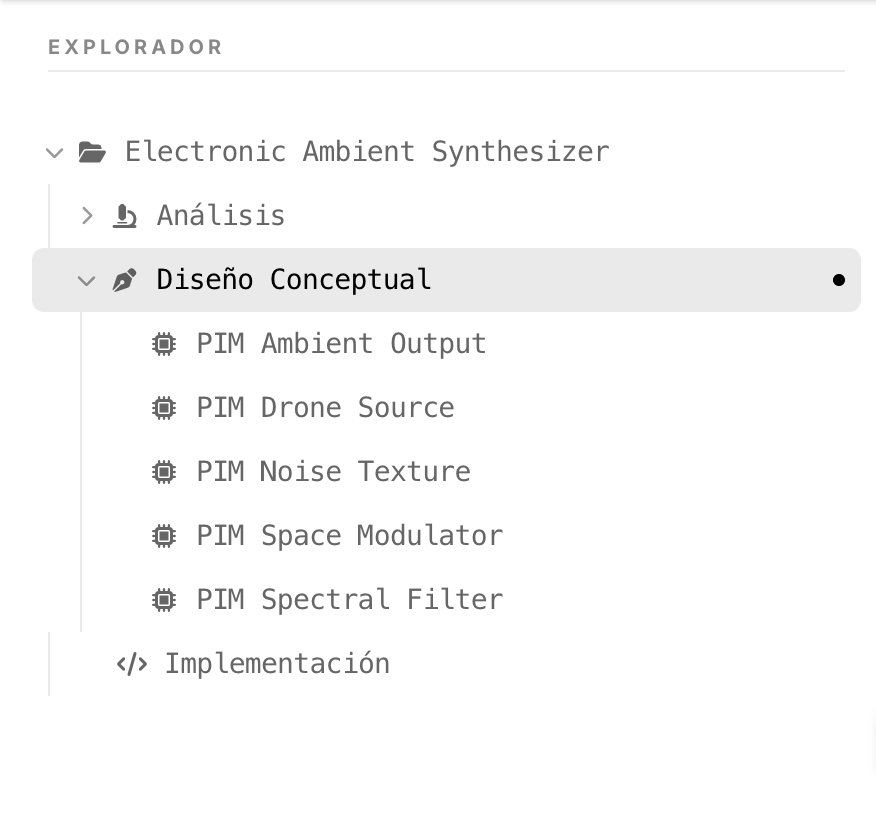
\includegraphics[width=0.4\textwidth]{imagenes/06_diseno/02_exploradorDisenoConceptual.png}
    \caption{Detalle de la rama de Diseño Conceptual en el explorador.}
\end{figure}

De modo paralelo al \textit{CIM}, el árbol del \textit{PIM} organiza las máquinas de diseño y las relaciones globales que definen el ecosistema orquestal desde una perspectiva de arquitectura de software.

\subsection{Creación y Gestión de Máquinas PIM}

\begin{figure}[!ht]
    \centering
    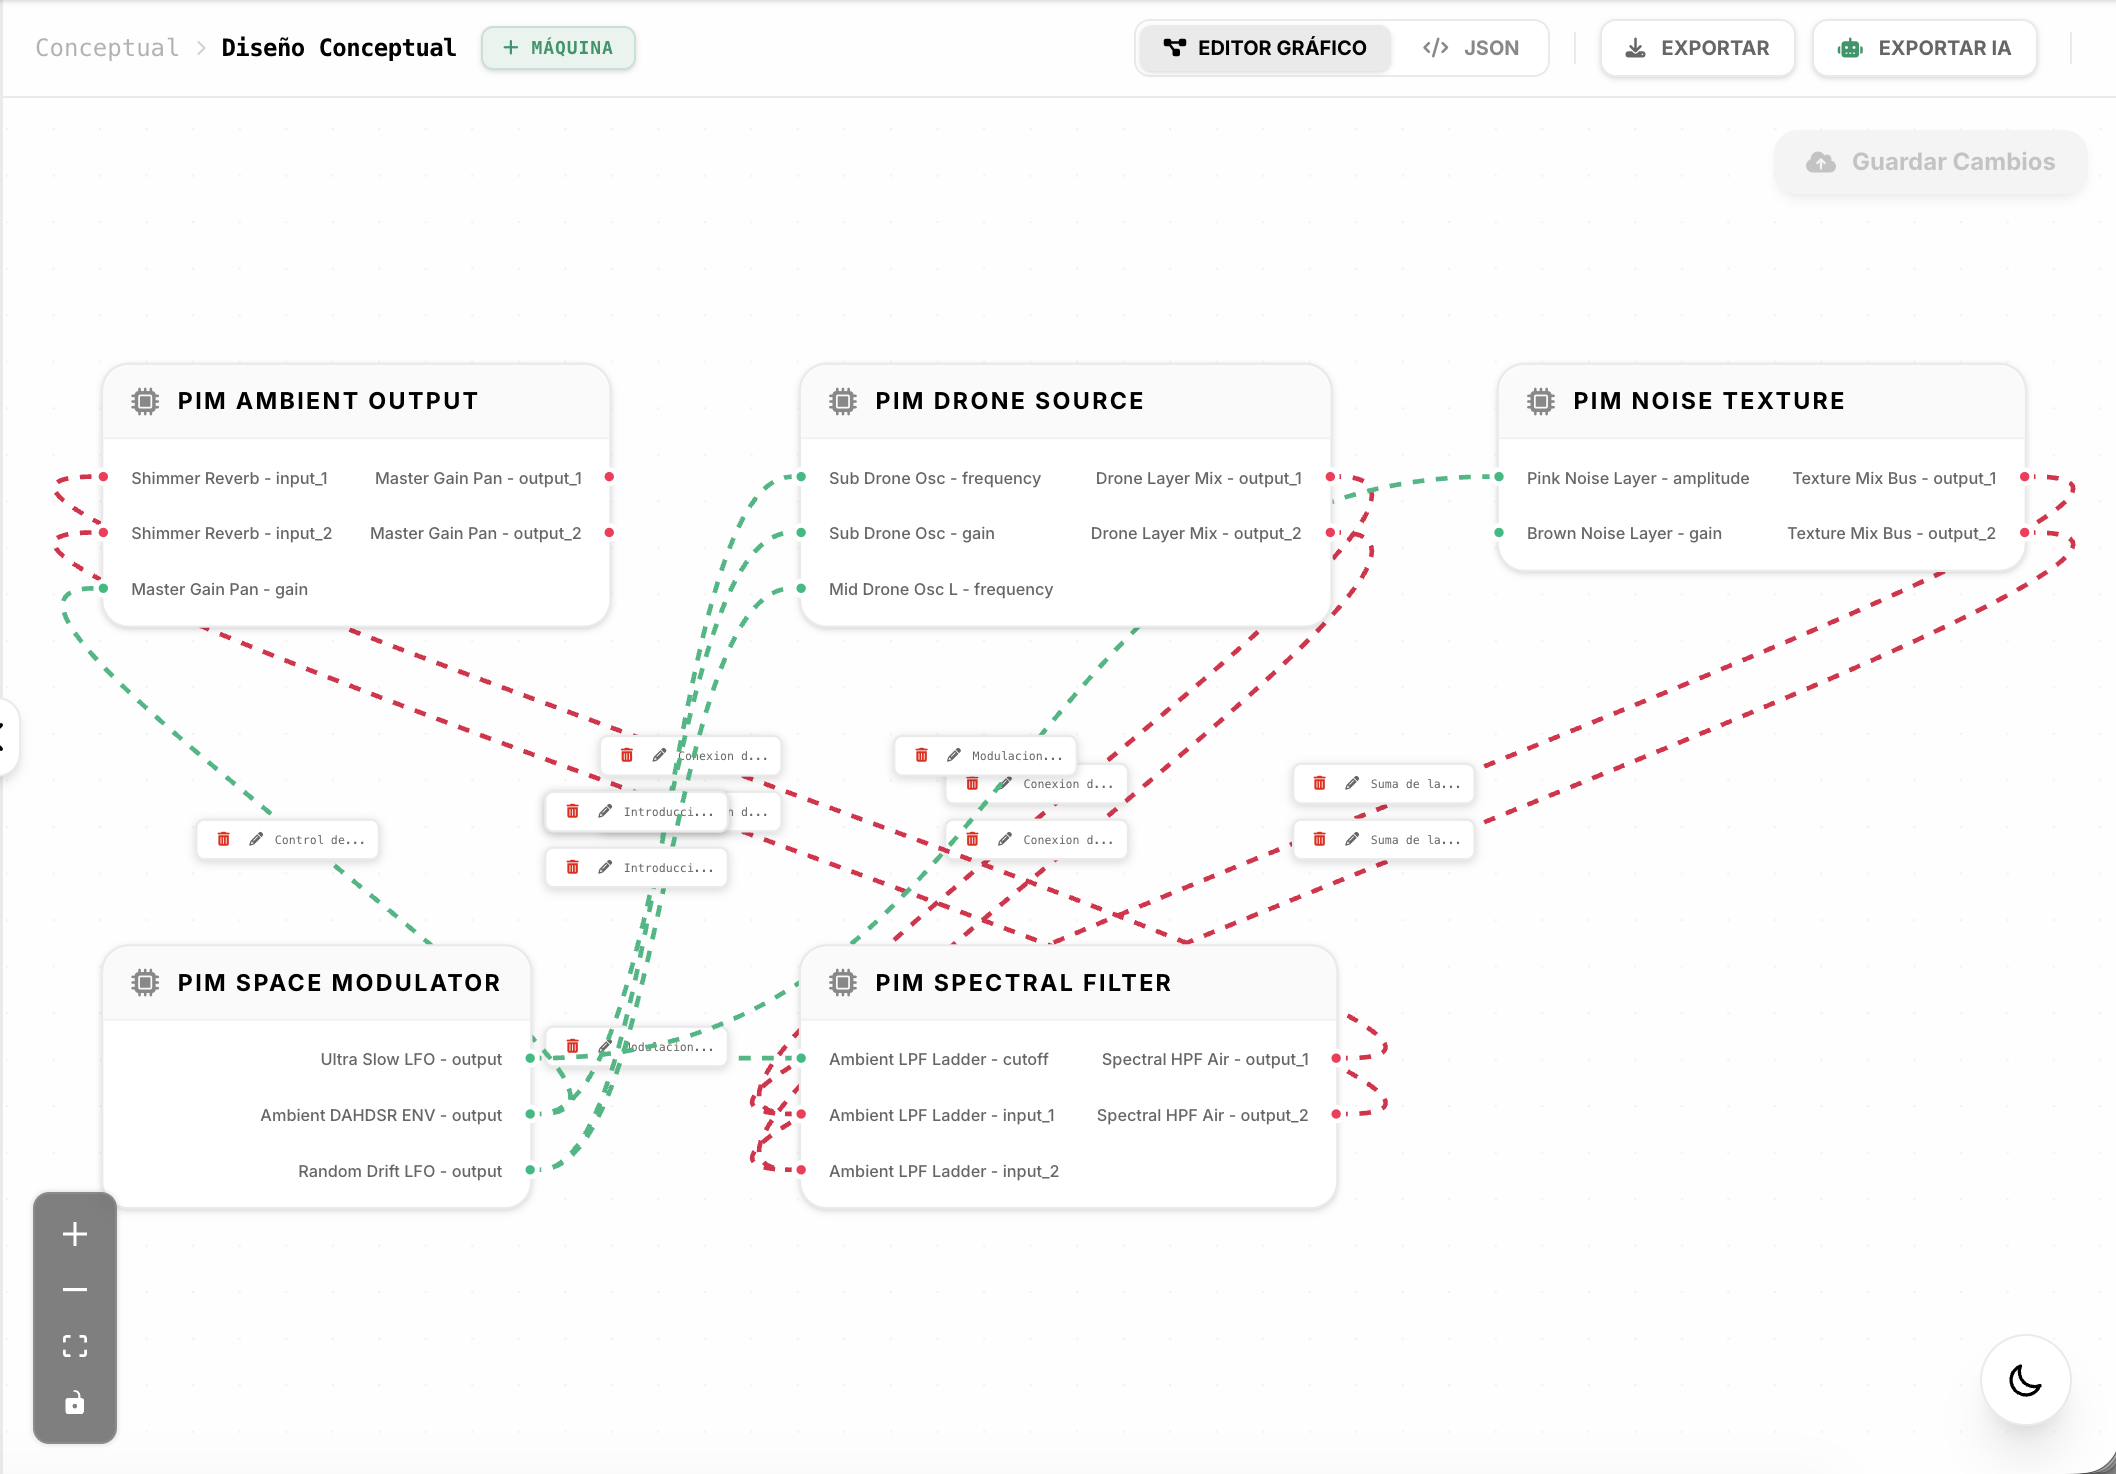
\includegraphics[width=\textwidth]{imagenes/06_diseno/03_visorEditorRelacionesPIM.png}
    \caption{Editor principal de relaciones en el nivel de Diseño Conceptual.}
\end{figure}

\begin{figure}[!ht]
    \centering
    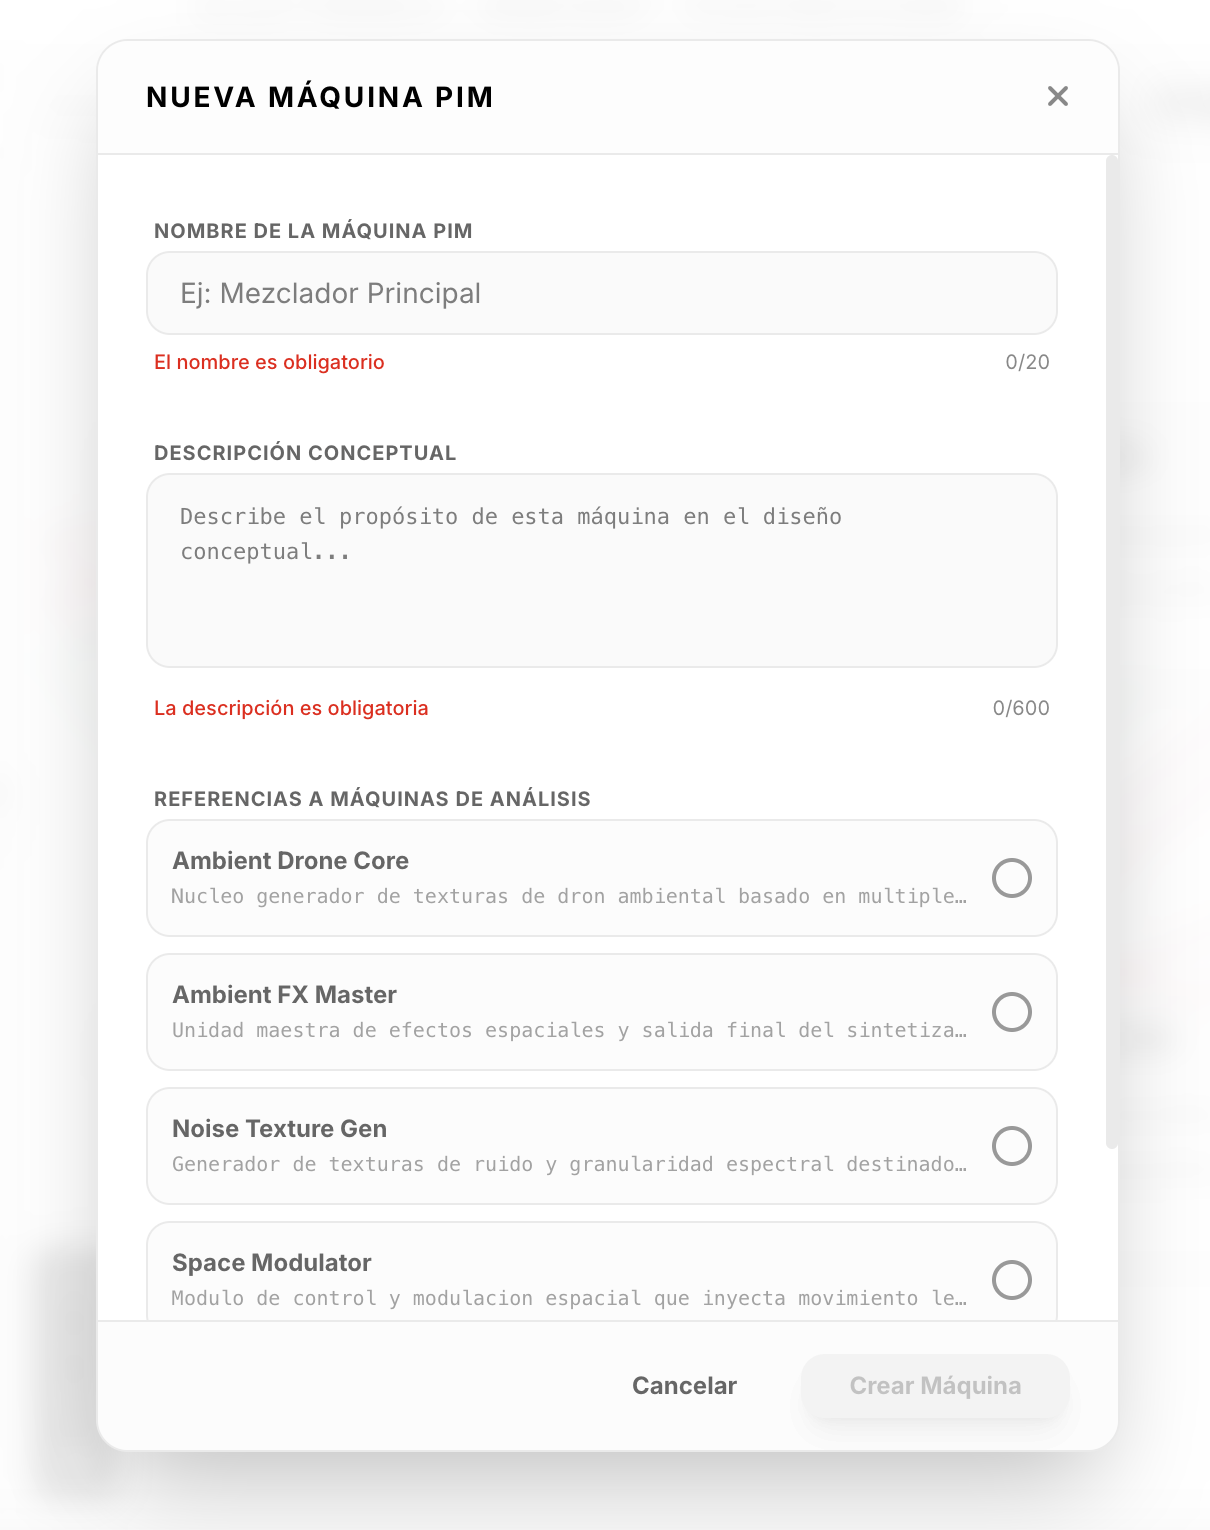
\includegraphics[width=0.6\textwidth]{imagenes/06_diseno/04_formularioCrearNuevaMaquinaPim.png}
    \caption{Formulario de instanciación de una nueva máquina PIM.}
\end{figure}

Desde el editor de relaciones del nivel \textit{PIM}, es posible crear nuevas máquinas de diseño. Crucialmente, estas máquinas \textit{PIM} a menudo referencian y especializan a las máquinas \textit{CIM} subyacentes, estableciendo el puente entre análisis y diseño definido por el lenguaje \textit{DSL}.

\section{Edición de Relaciones PIM}

La interactividad y la edición avanzada son pilares fundamentales para establecer la red de diseño computacional.

\subsection{Visor Gráfico y Edición Topológica}

\begin{figure}[!ht]
    \centering
    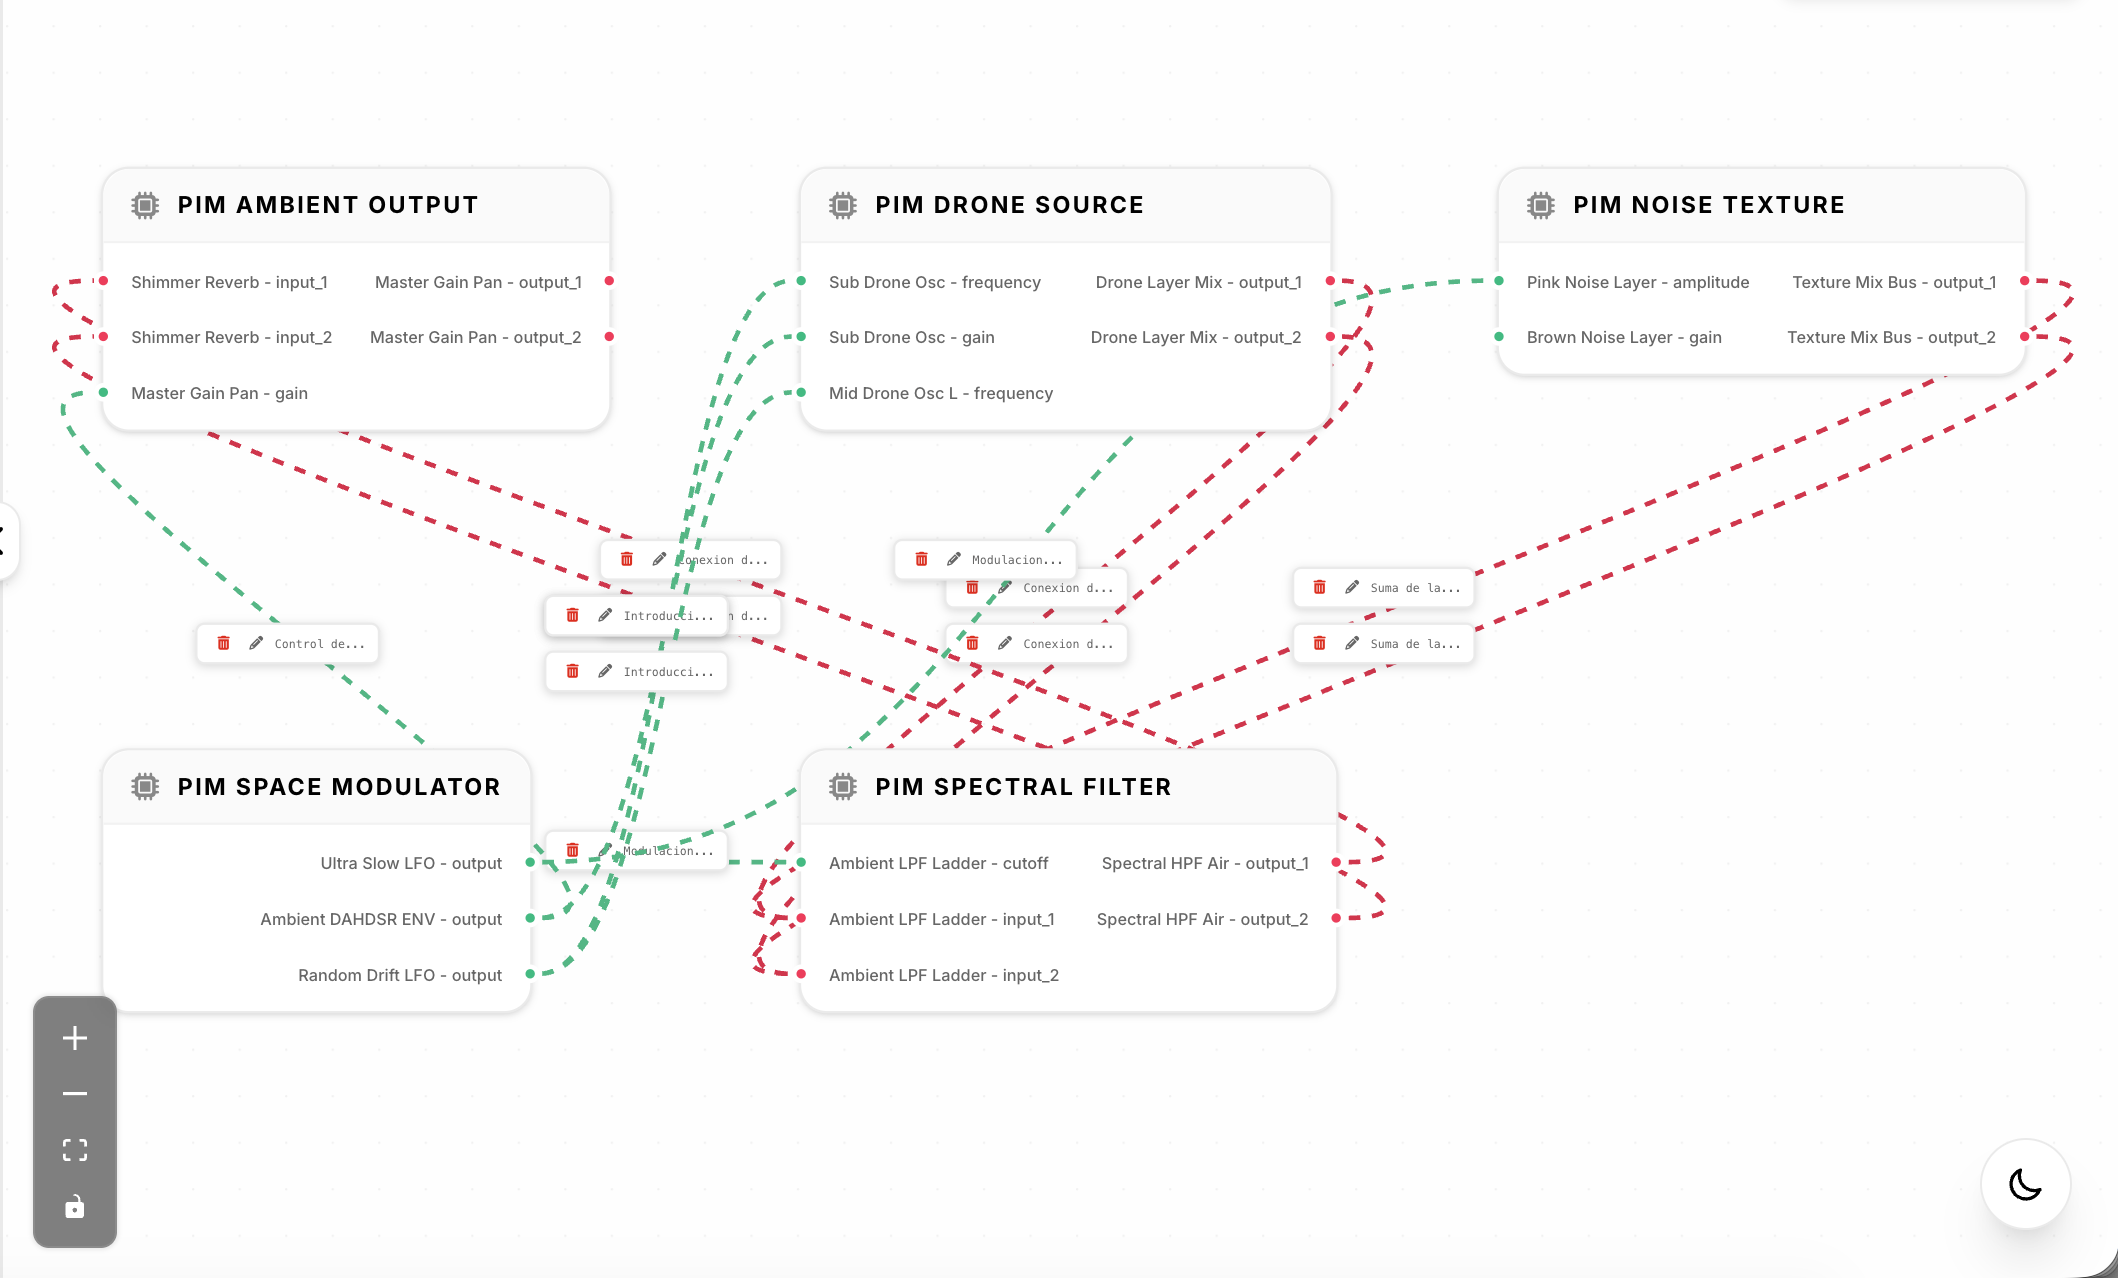
\includegraphics[width=\textwidth]{imagenes/06_diseno/05_visorGraficoRelacionesPim.png}
    \caption{Visor gráfico de la red de relaciones PIM.}
\end{figure}

El grafo de \textit{PIM} revela la complejidad de la arquitectura diseñada. A diferencia del \textit{CIM}, las conexiones en esta fase suelen representar flujos de datos de audio concretos, señales de control y eventos del sistema.

\begin{figure}[!ht]
    \centering
    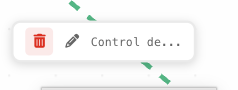
\includegraphics[width=0.5\textwidth]{imagenes/06_diseno/06_edicionGraficasAristasPim.png}
    \caption{Controles contextuales para la edición de aristas en el visor gráfico.}
\end{figure}

\begin{figure}[!ht]
    \centering
    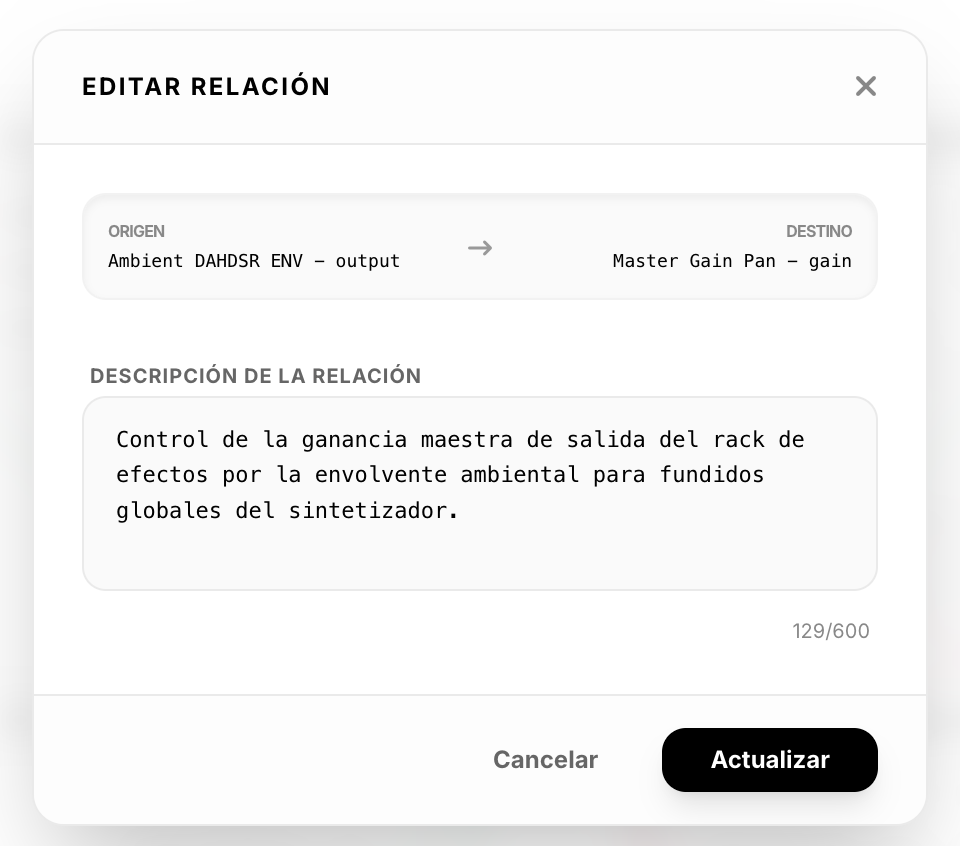
\includegraphics[width=0.6\textwidth]{imagenes/06_diseno/07_formularioEdicionGraficoAristasPim.png}
    \caption{Formulario rápido para ajustar la configuración de una conexión.}
\end{figure}

El entorno gráfico no es solo de consulta. Integrados en los elementos visuales, se encuentran controles que permiten editar directamente las propiedades de las aristas (como asignar tipos de puerto o alterar cardinalidades) sin necesidad de recurrir al código.

\begin{figure}[!ht]
    \centering
    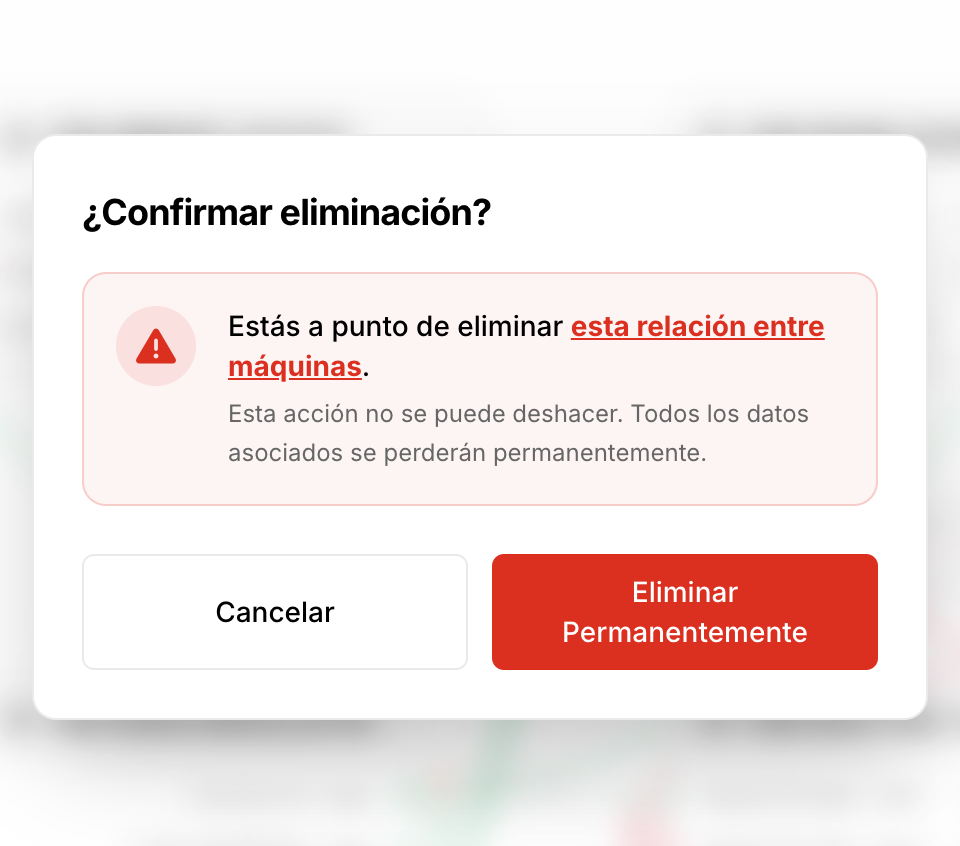
\includegraphics[width=0.6\textwidth]{imagenes/06_diseno/08_eliminarGraficamenteAristaPim.png}
    \caption{Confirmación al eliminar una arista directamente desde el entorno gráfico.}
\end{figure}

La topología puede ser modificada interactivamente, incluyendo la eliminación de enlaces, siempre mediada por ventanas de confirmación para evitar acciones destructivas accidentales.

\subsection{Edición mediante Código JSON}

\begin{figure}[!ht]
    \centering
    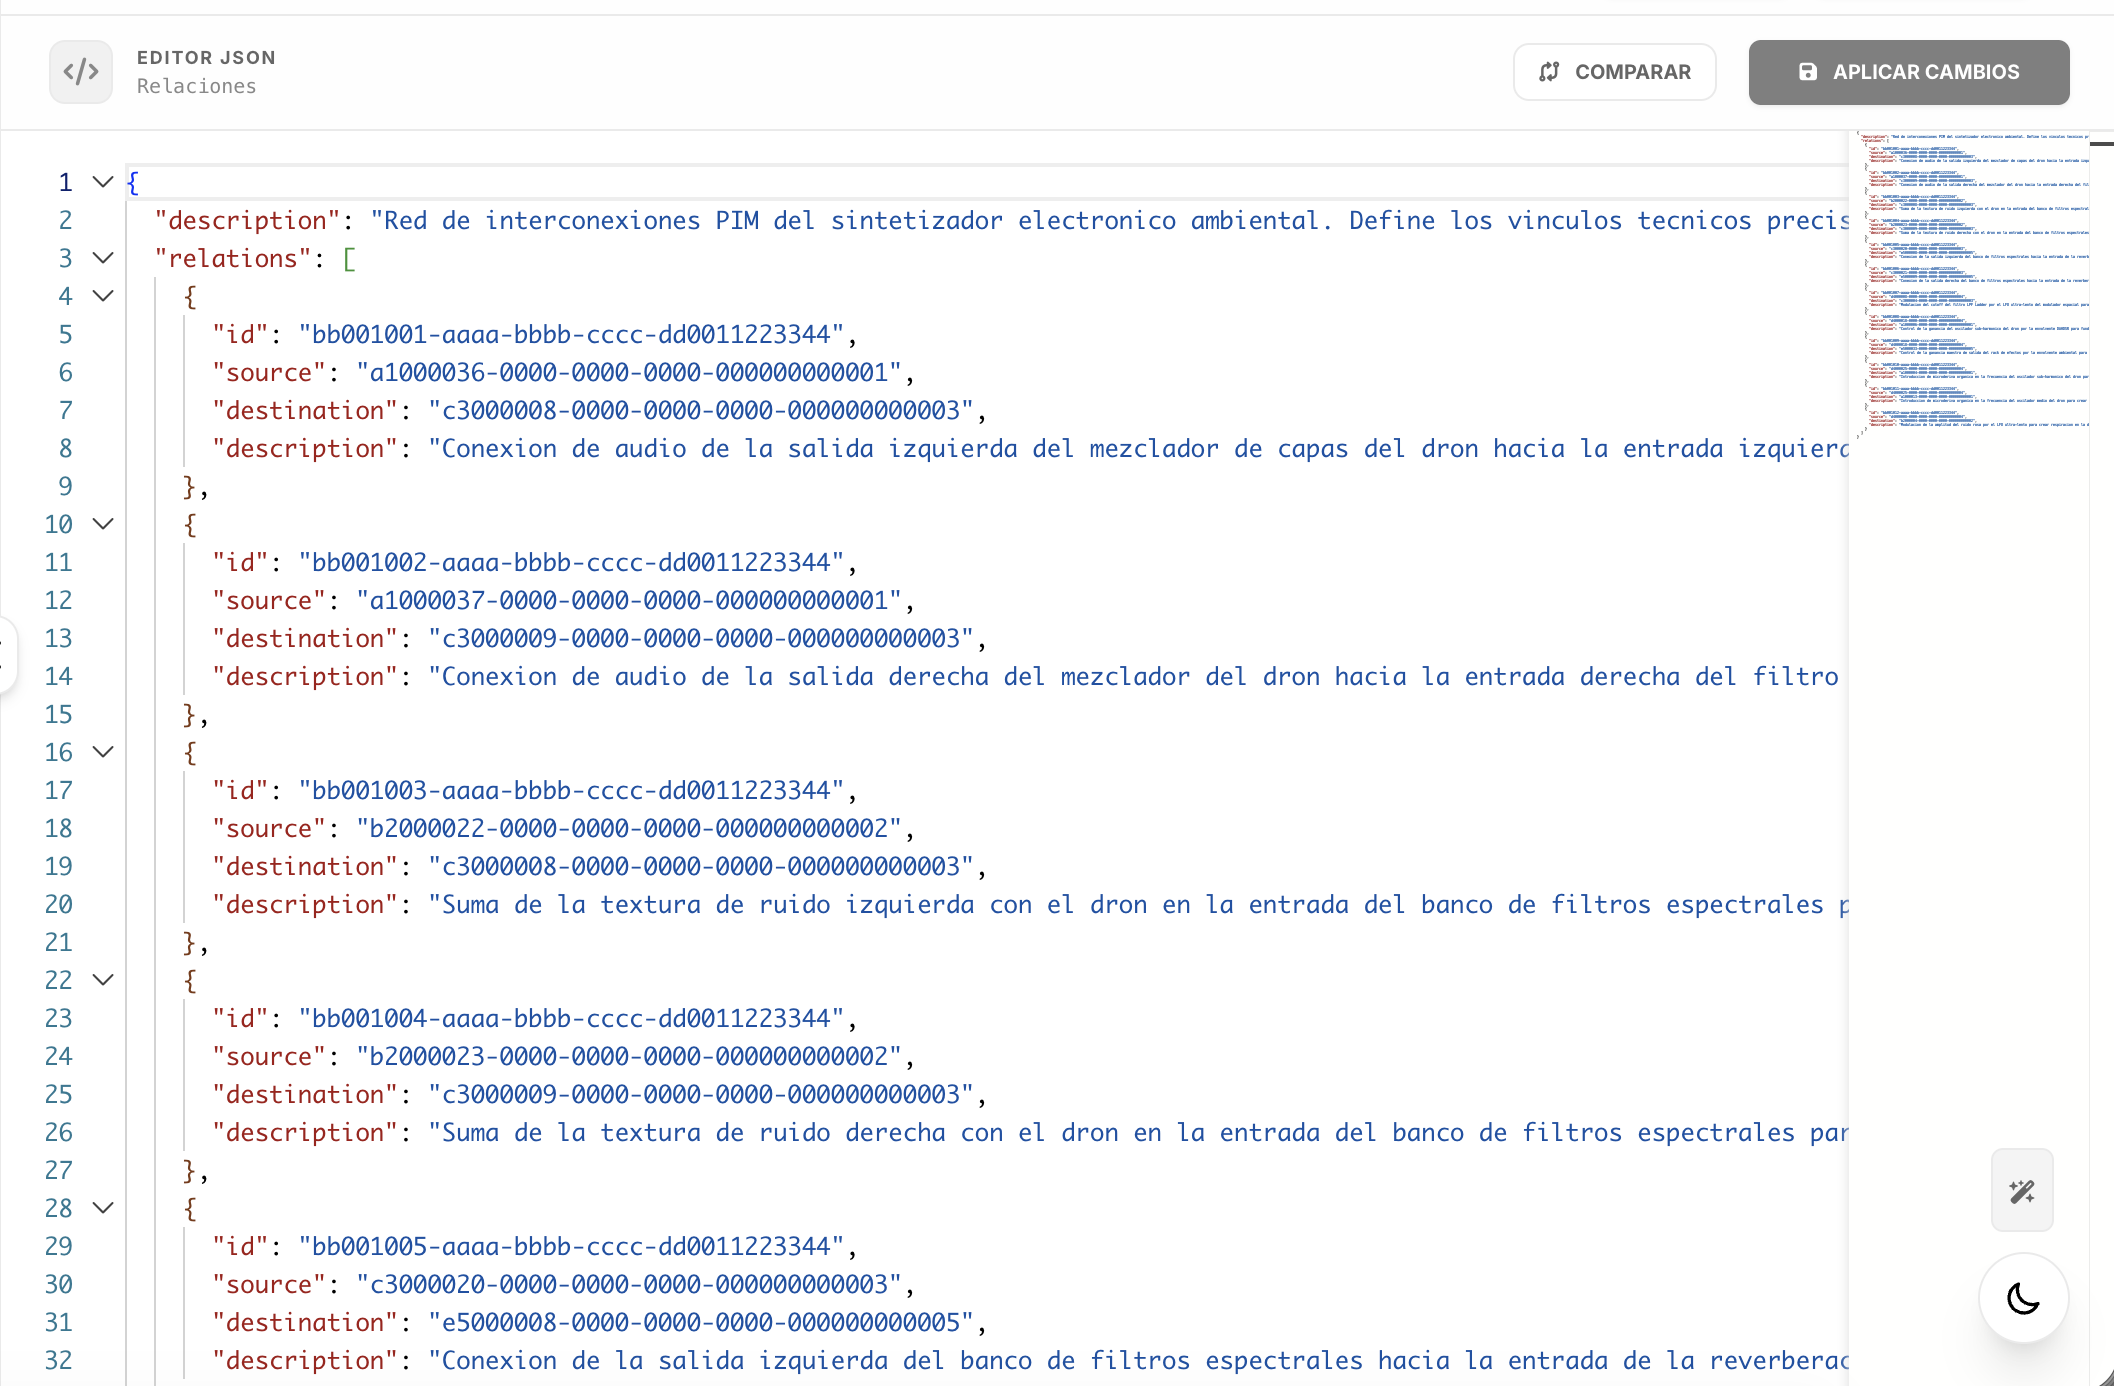
\includegraphics[width=\textwidth]{imagenes/06_diseno/09_edicionJsonRelacionesPim.png}
    \caption{Editor de código JSON para relaciones PIM.}
\end{figure}

Para manipulaciones granulares y ajustes de la estructura \textit{DSL}, se dispone del editor \textit{JSON} enfocado al modelo \textit{PIM}.

\begin{figure}[!ht]
    \centering
    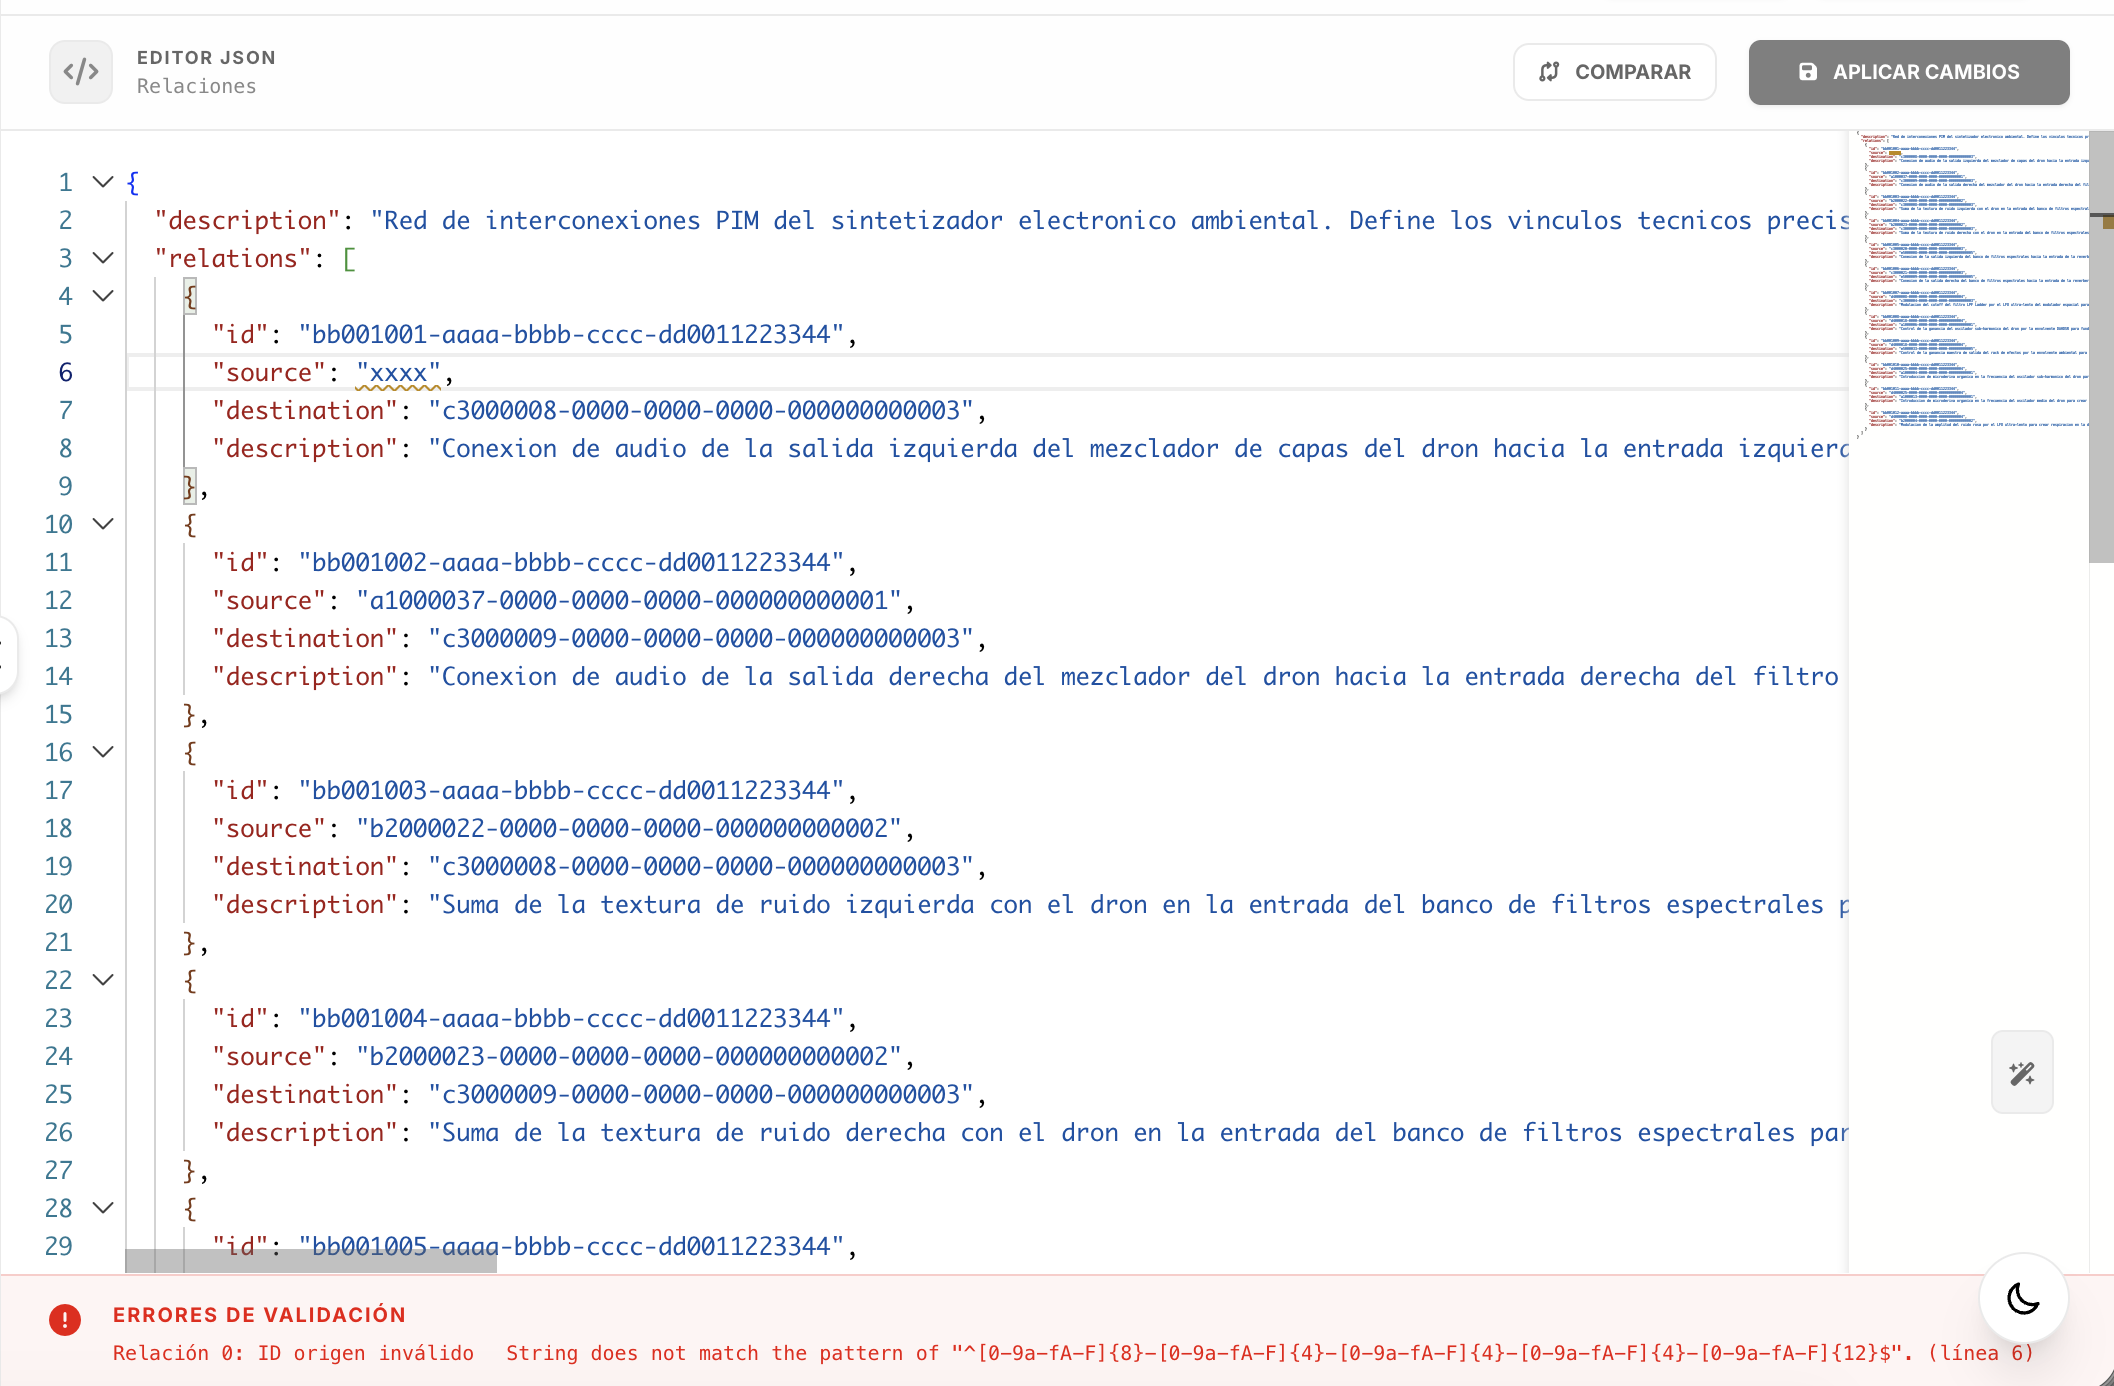
\includegraphics[width=\textwidth]{imagenes/06_diseno/10_edicionJsonRelacionesPimValidacion.png}
    \caption{Validación de esquema y reglas de diseño en el editor JSON.}
\end{figure}

Este editor incorpora capacidades de validación estrictas, verificando que el código cumple con las normativas del metamodelo \textit{PIM}, resaltando cualquier inconsistencia estructural antes de su almacenamiento.

\begin{figure}[!ht]
    \centering
    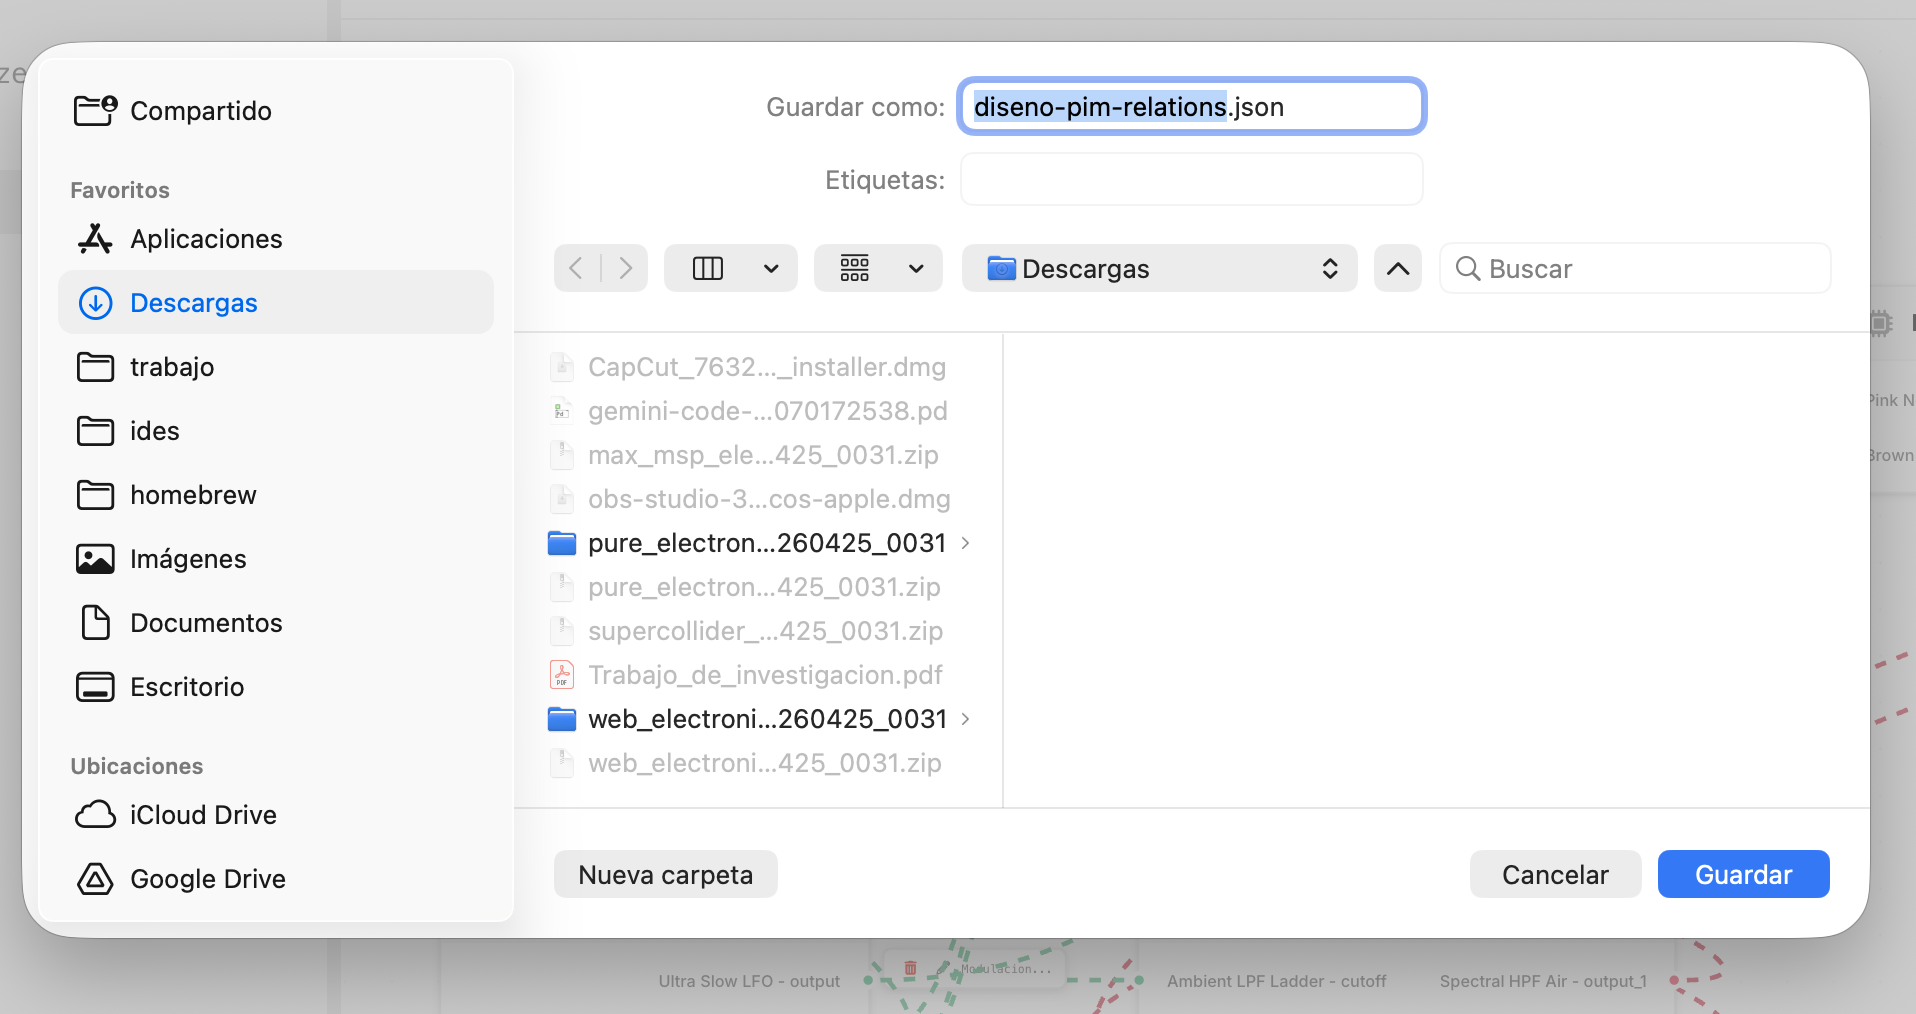
\includegraphics[width=0.6\textwidth]{imagenes/06_diseno/11_exportarJsonRelacionesPim.png}
    \caption{Opción para exportar el modelo PIM a nivel de relaciones.}
\end{figure}

\begin{figure}[!ht]
    \centering
    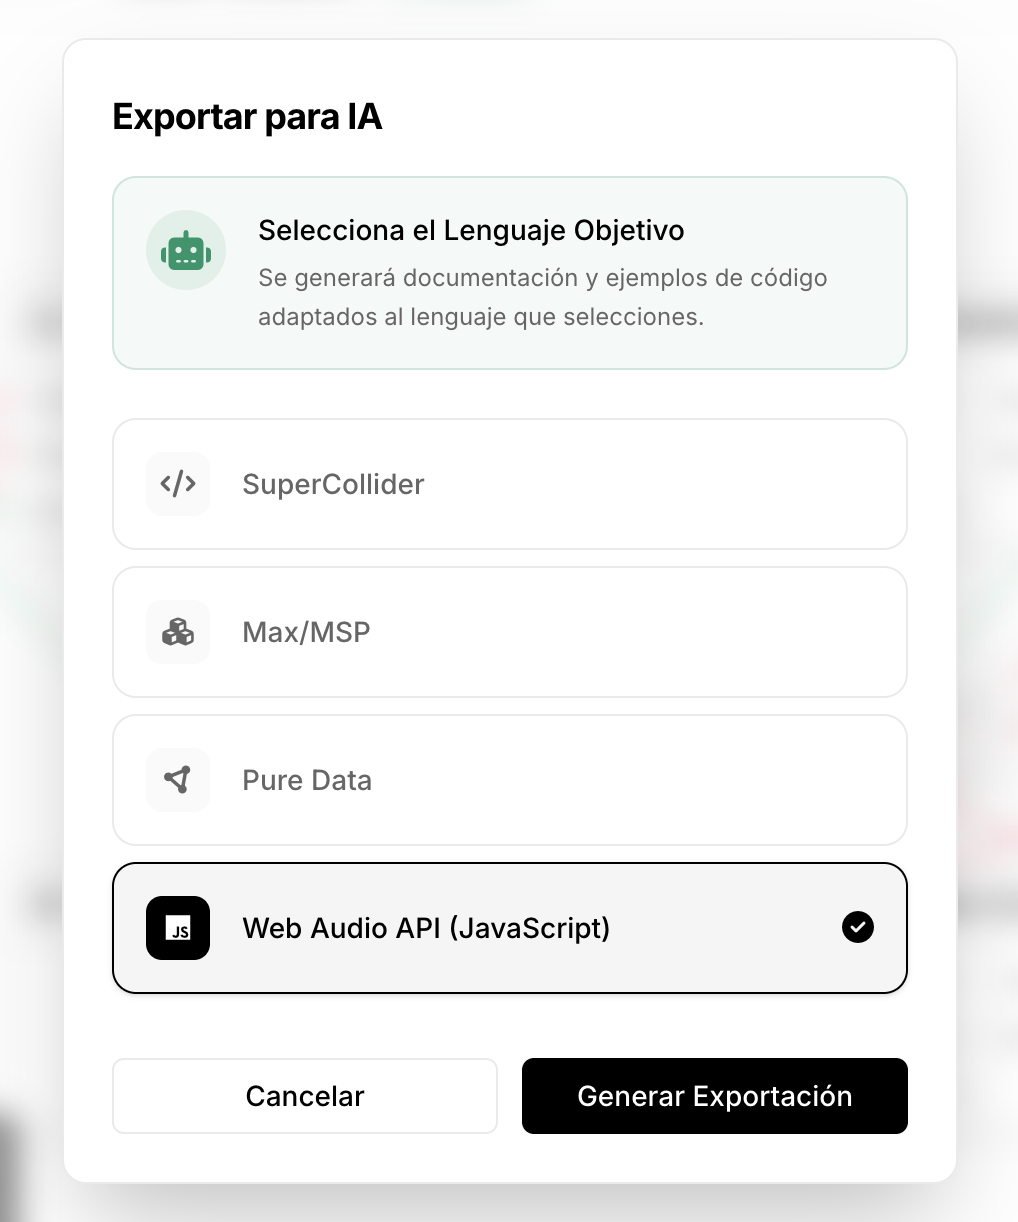
\includegraphics[width=0.4\textwidth]{imagenes/06_diseno/12_exportarParaIA.png}
    \caption{Opción de exportación de contexto para Inteligencia Artificial.}
\end{figure}

Junto a la exportación estándar del fichero \textit{JSON}, el nivel \textit{PIM} habilita utilidades avanzadas como la ``Exportación para IA'', diseñada para extraer el contexto del proyecto y facilitar la asistencia de herramientas generativas externas.

\section{Configuración de Máquinas PIM}

\begin{figure}[!ht]
    \centering
    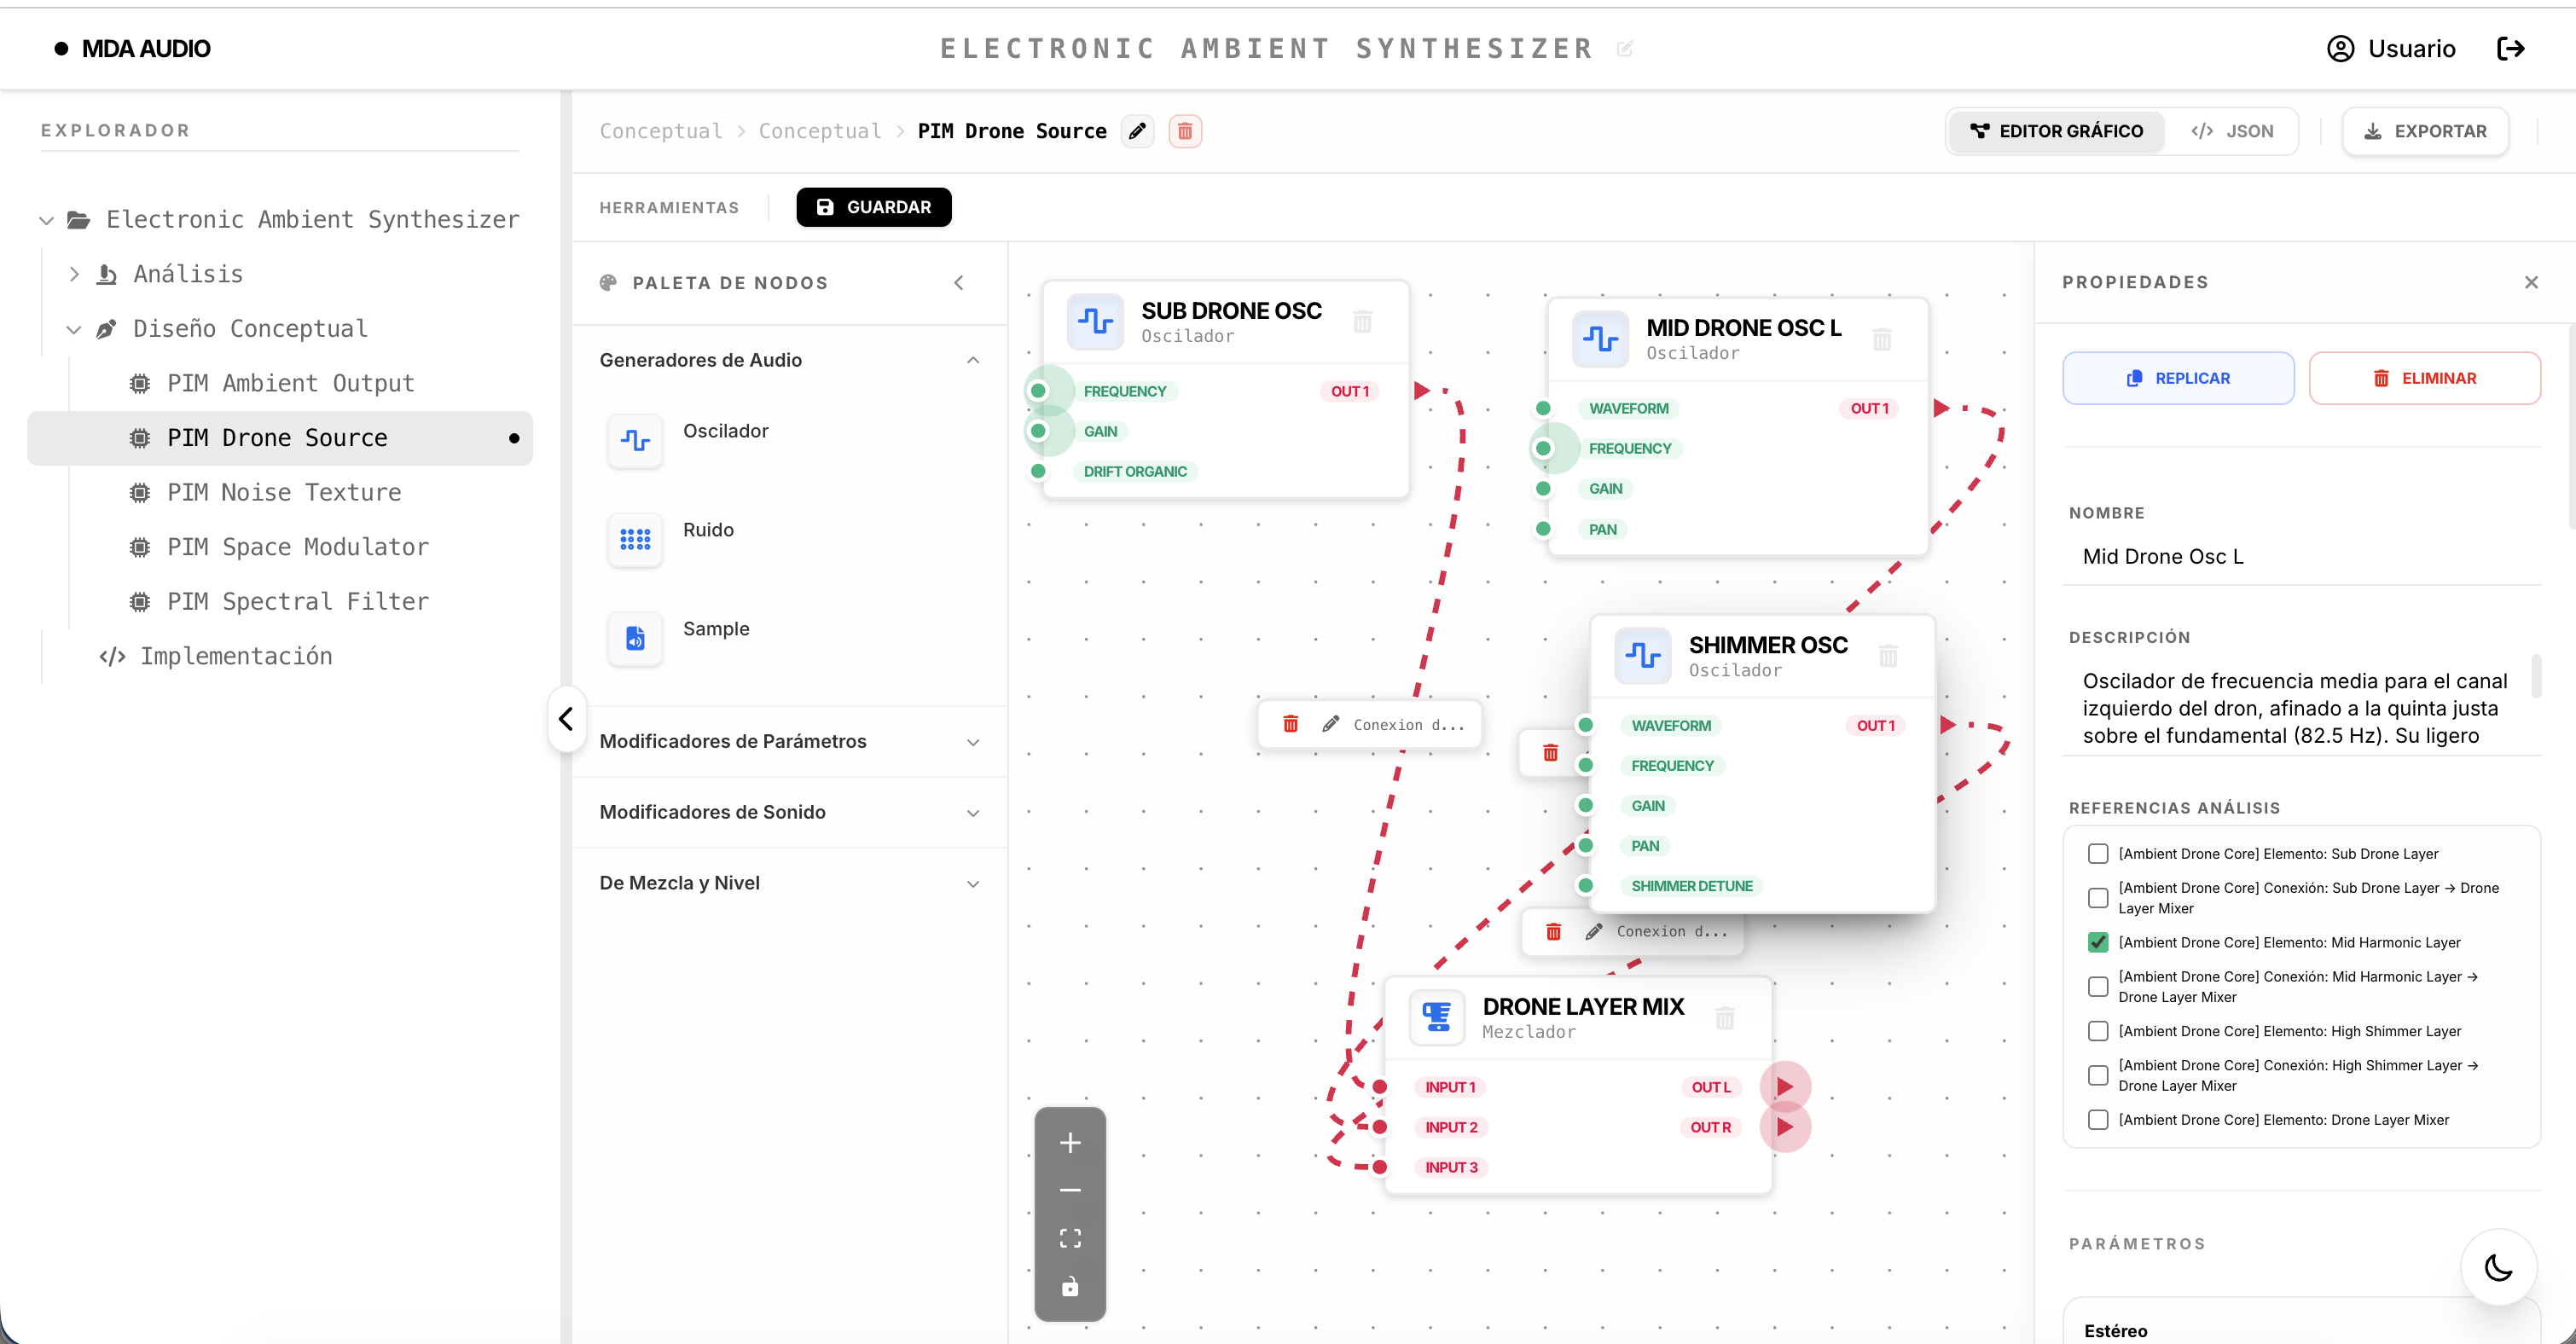
\includegraphics[width=\textwidth]{imagenes/06_diseno/13_pantallaMaquinaPim.png}
    \caption{Pantalla de detalle para la configuración de una máquina PIM específica.}
\end{figure}

Seleccionando una máquina desde el explorador bajo la rama \textit{PIM}, se accede a su entorno de configuración detallada.

\begin{figure}[!ht]
    \centering
    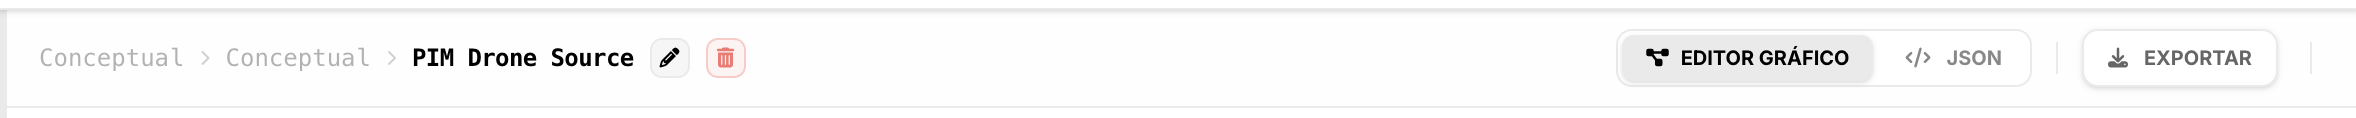
\includegraphics[width=\textwidth]{imagenes/06_diseno/14_barraMaquinaPim.png}
    \caption{Barra de herramientas contextual para la gestión de la máquina PIM.}
\end{figure}

\begin{figure}[!ht]
    \centering
    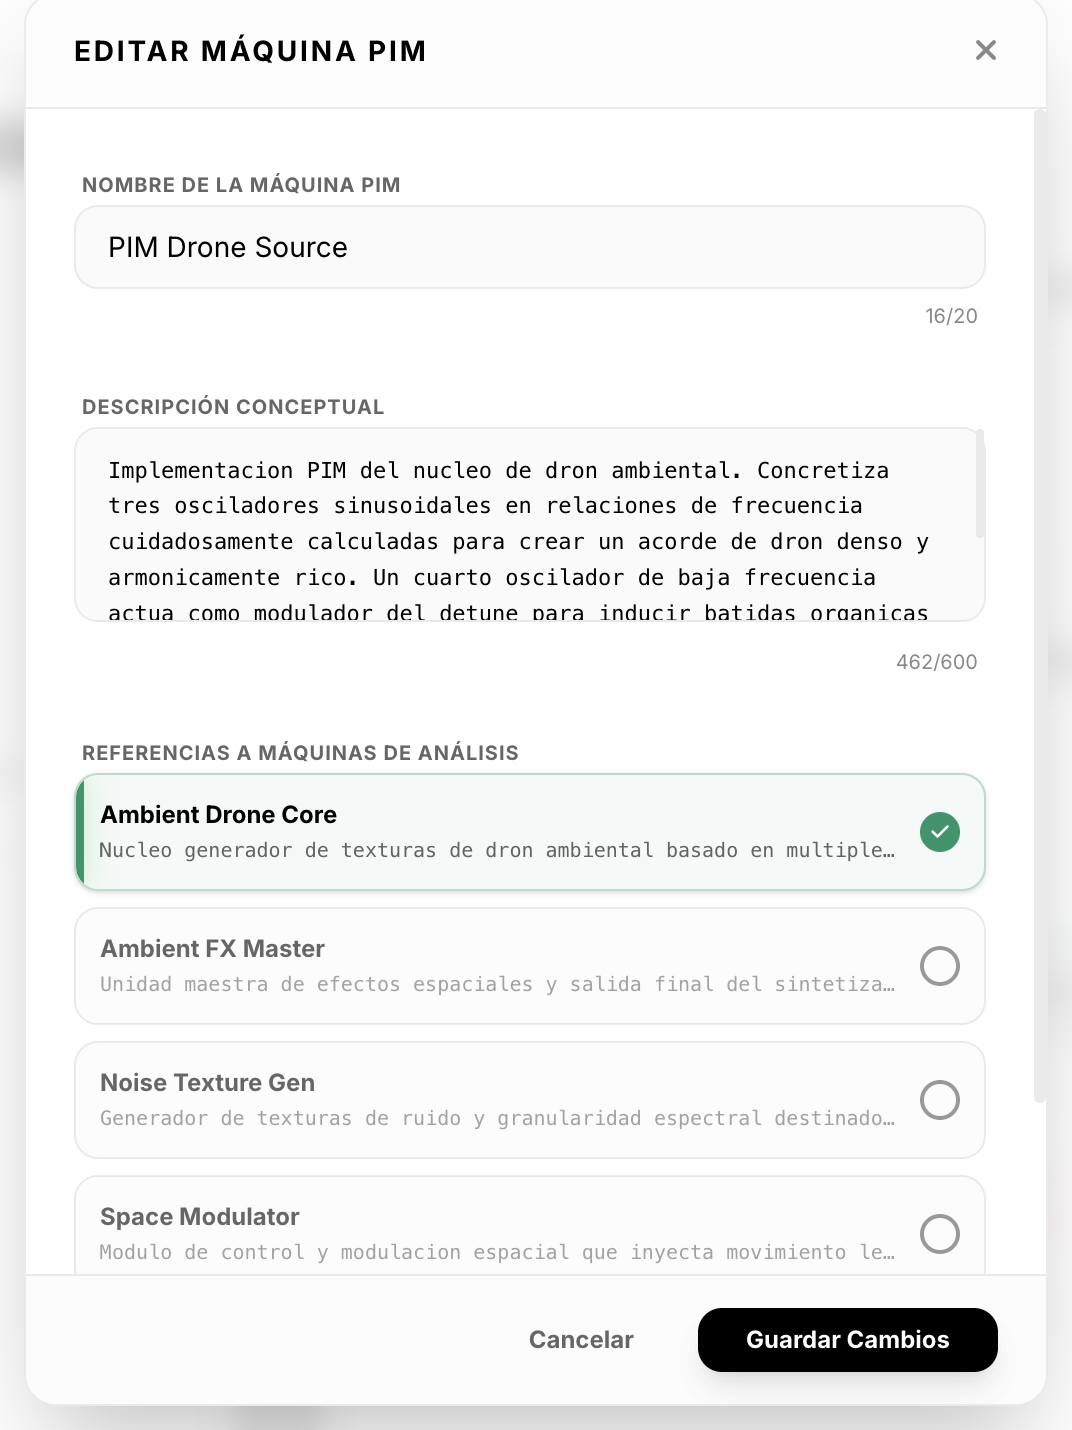
\includegraphics[width=0.6\textwidth]{imagenes/06_diseno/15_editarMaquinaPim.png}
    \caption{Formulario para modificar las propiedades principales de la máquina.}
\end{figure}

La barra de herramientas de la máquina permite acceder rápidamente a su edición, posibilitando ajustar su identificador o actualizar sus referencias a elementos del modelo \textit{CIM}.

\begin{figure}[!ht]
    \centering
    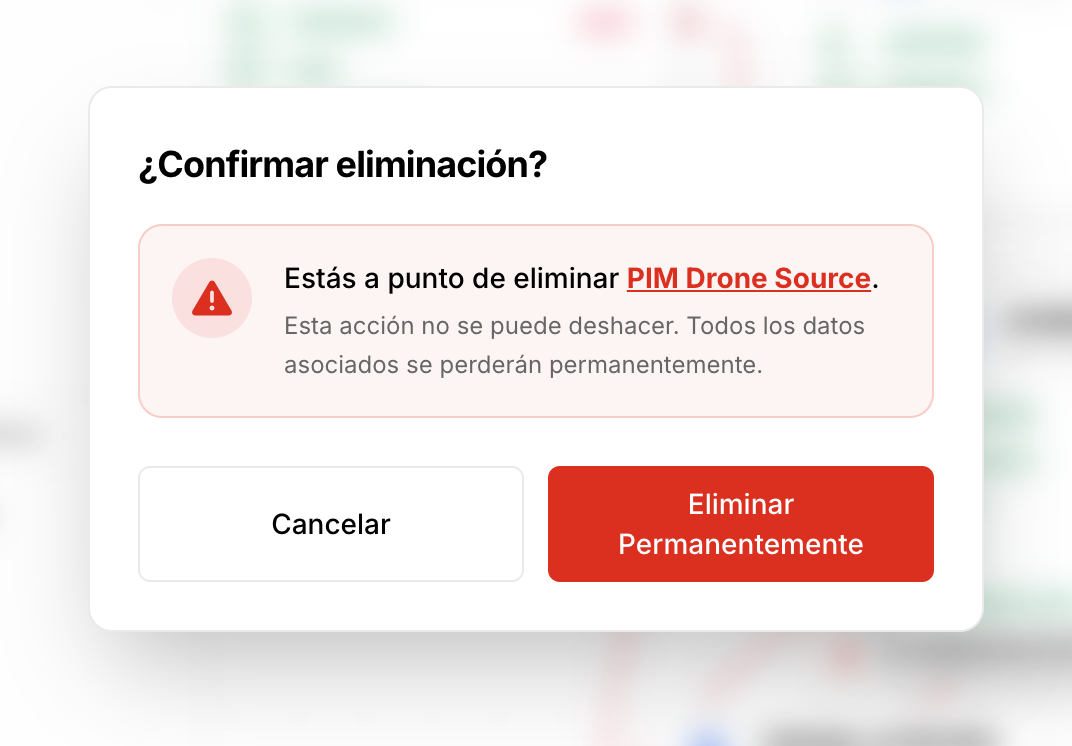
\includegraphics[width=0.6\textwidth]{imagenes/06_diseno/16_eliminarMaquinaPim.png}
    \caption{Proceso de eliminación segura de una máquina PIM.}
\end{figure}

Si la máquina ya no es necesaria en el diseño, se puede eliminar mediante la correspondiente validación de seguridad.

\subsection{Validación y Control de Versiones Interno}

\begin{figure}[!ht]
    \centering
    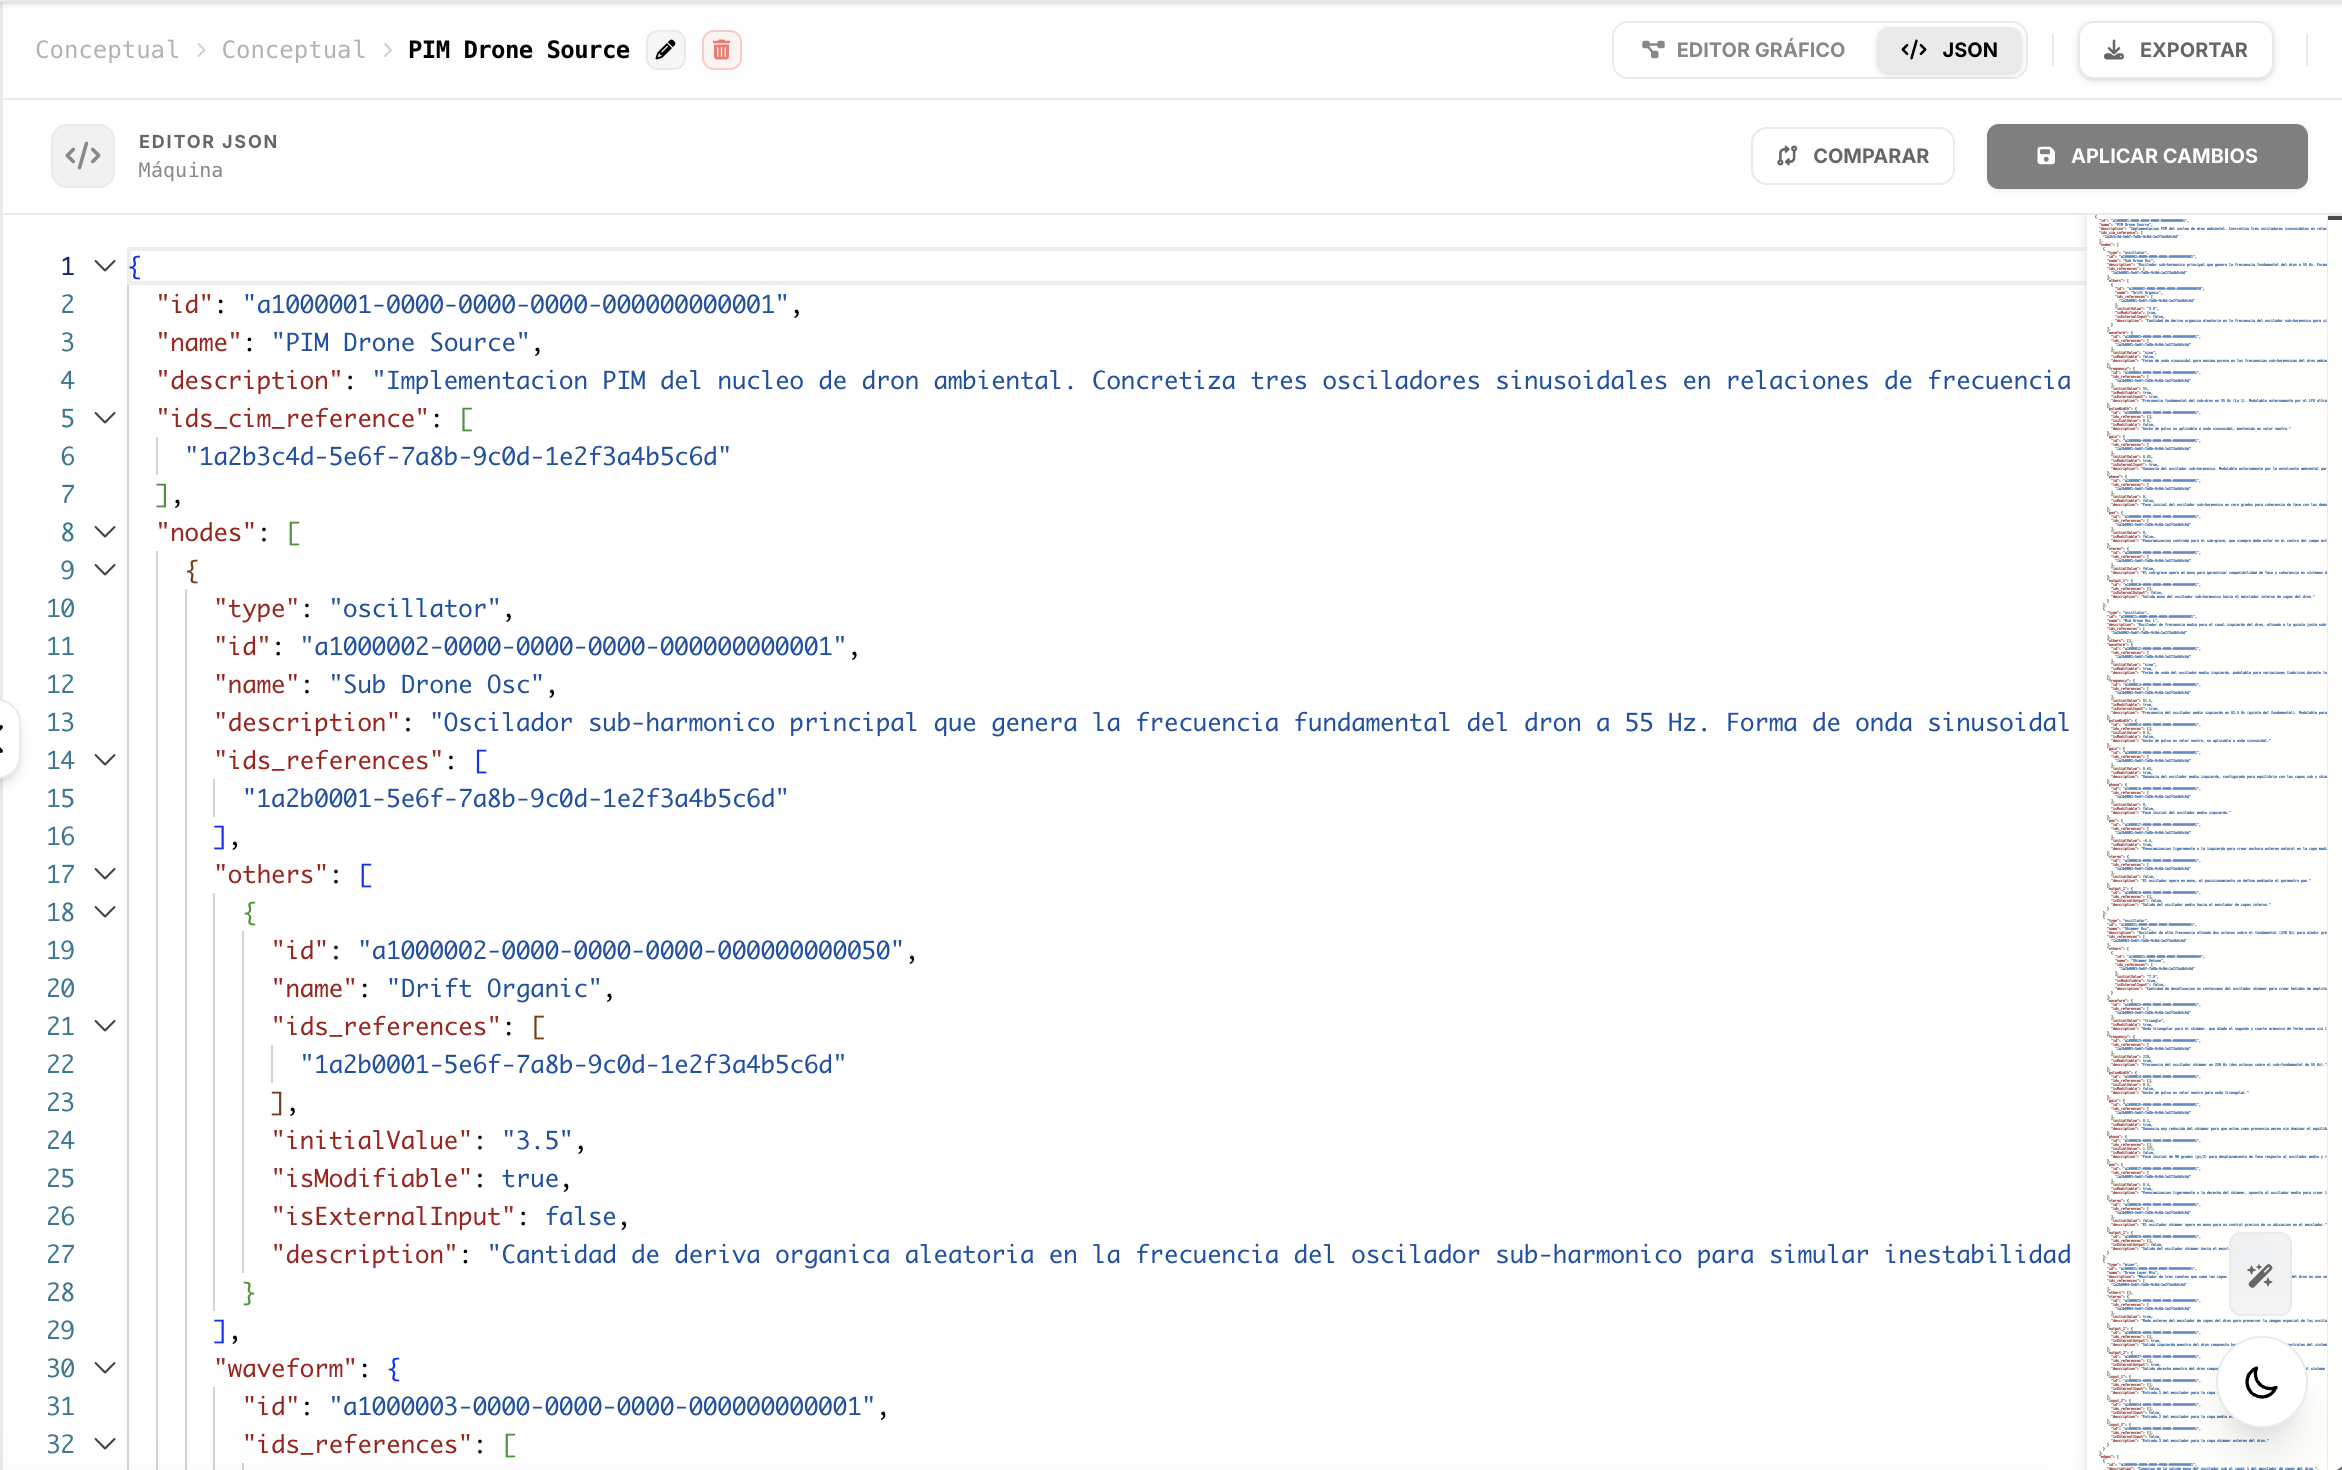
\includegraphics[width=\textwidth]{imagenes/06_diseno/17_edicionJsonMaquinaPim.png}
    \caption{Editor de código de la definición interna de la máquina PIM.}
\end{figure}

\begin{figure}[!ht]
    \centering
    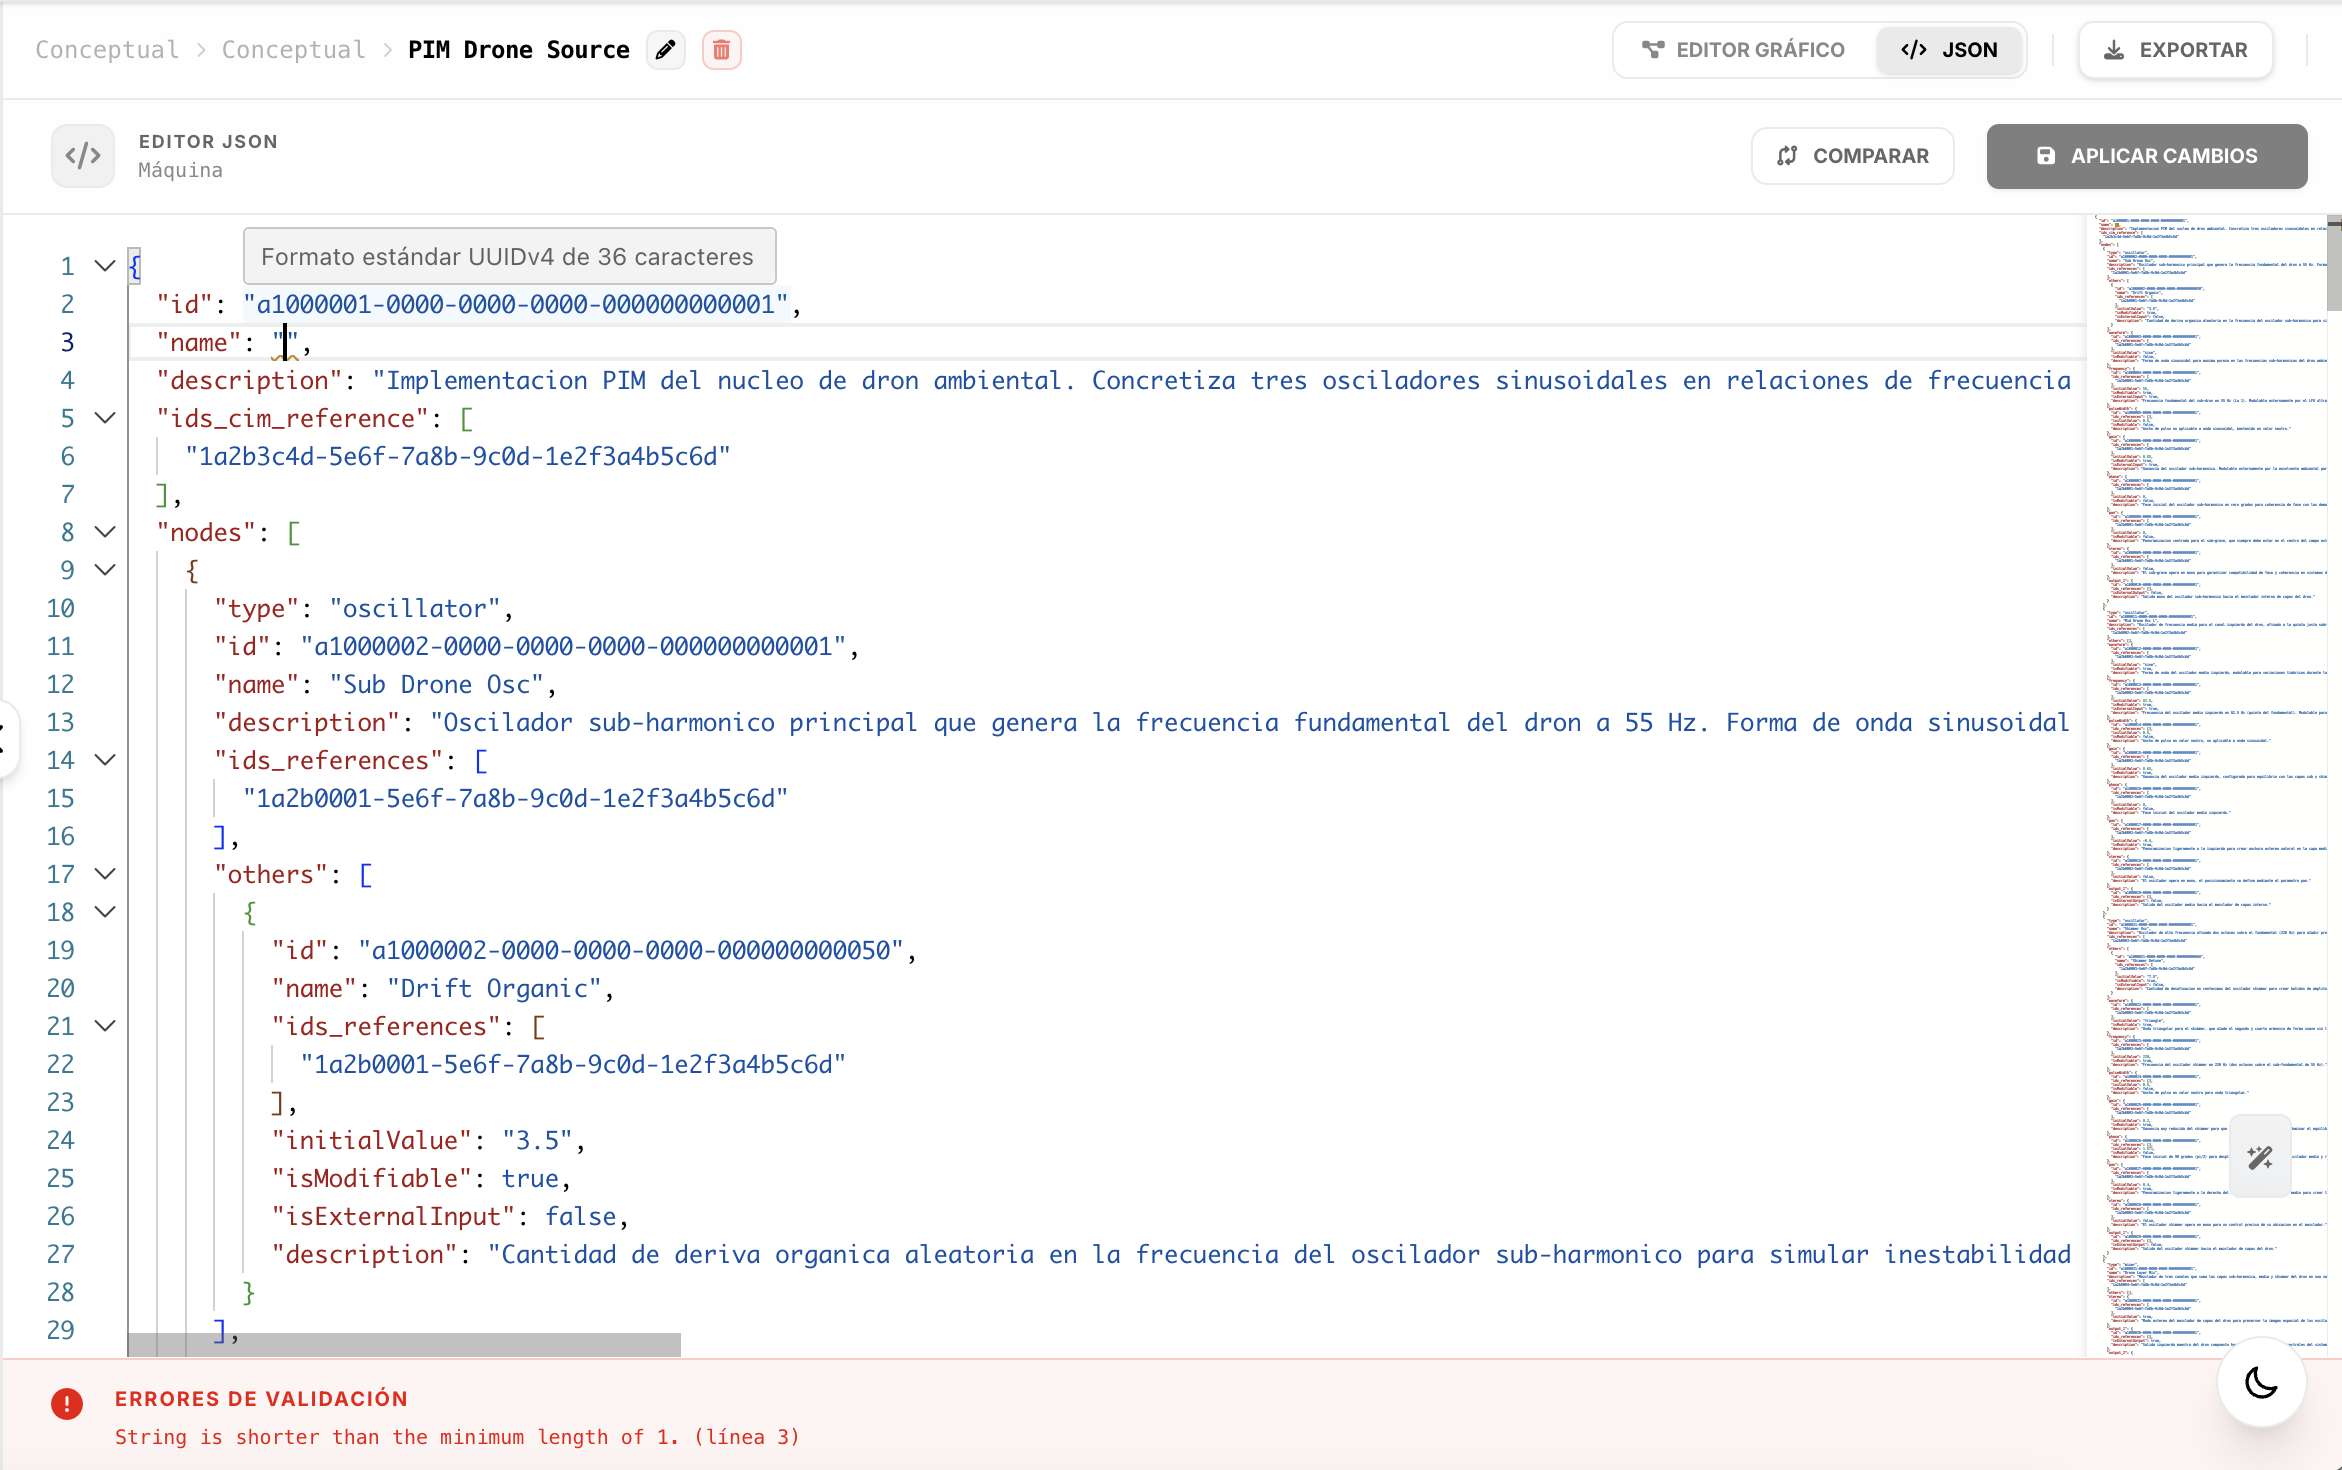
\includegraphics[width=\textwidth]{imagenes/06_diseno/18_edicionJsonMaquinaPimValidacion.png}
    \caption{Detección de errores y comprobación de integridad en la máquina PIM.}
\end{figure}

El modelado profundo de la máquina se realiza mediante su editor de código. Las reglas del dominio validan la consistencia de los bloques lógicos de síntesis, señalando errores sintácticos o discrepancias con las definiciones conceptuales.

\begin{figure}[!ht]
    \centering
    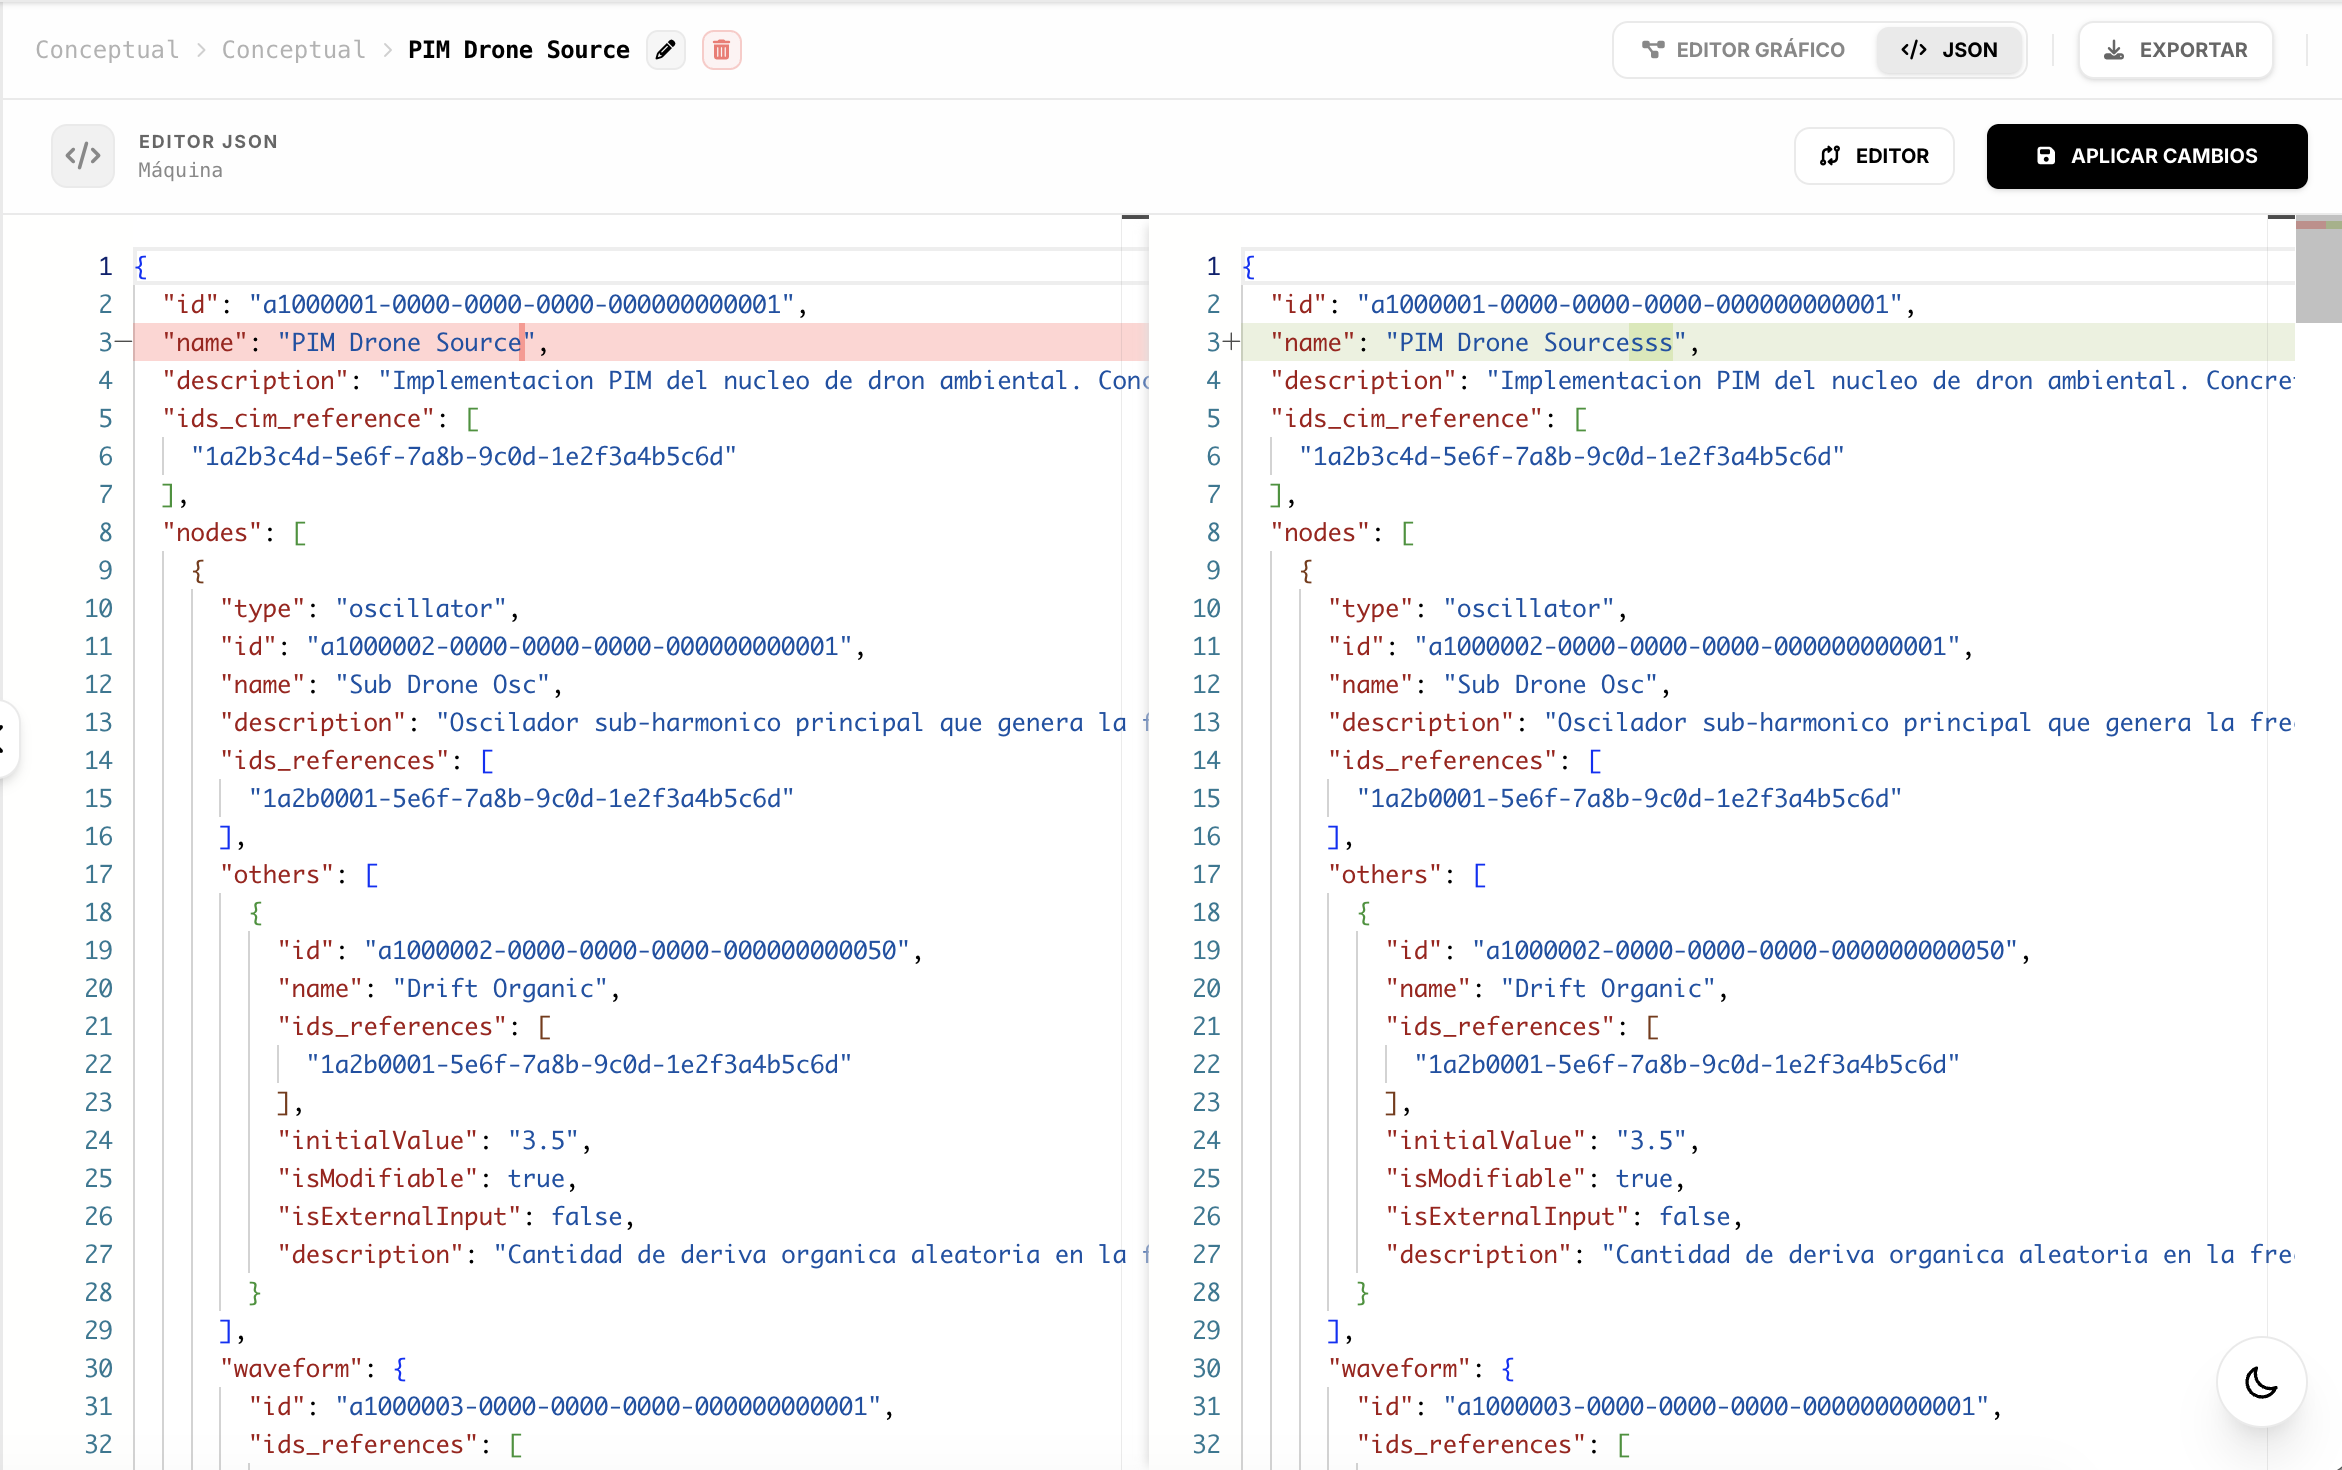
\includegraphics[width=\textwidth]{imagenes/06_diseno/19_edicionJsonMaquinaPimComparacion.png}
    \caption{Uso de la herramienta Diff para auditar cambios en la configuración interna.}
\end{figure}

\begin{figure}[!ht]
    \centering
    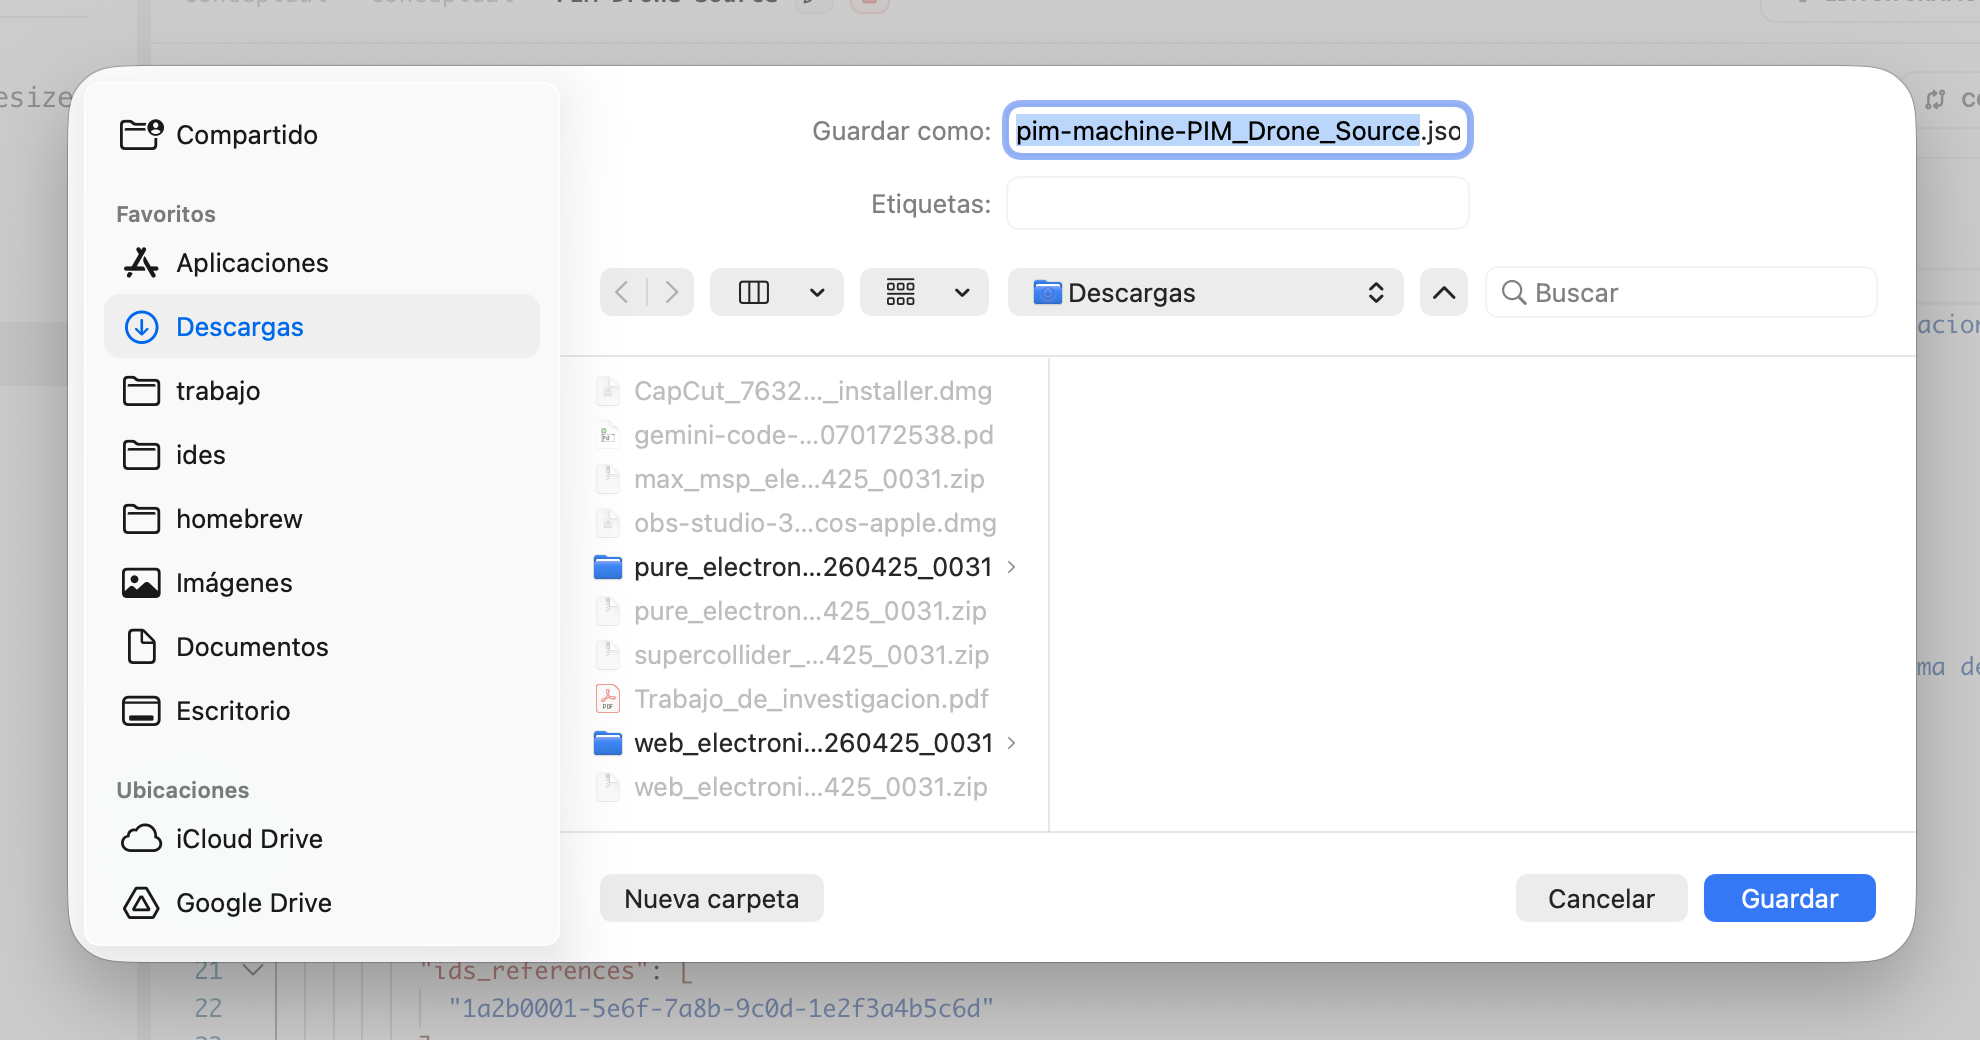
\includegraphics[width=0.6\textwidth]{imagenes/06_diseno/20_exportarJsonMaquinaPim.png}
    \caption{Exportación individual del código fuente de la máquina PIM.}
\end{figure}

Las herramientas de auditoría visual (\textit{diff}) y las capacidades de exportación se aplican también a nivel de máquina, proveyendo al arquitecto de software un control absoluto sobre el ciclo de vida del diseño computacional de cada componente.

\chapter{Elementos de Diseño}

Cada elemento dentro del diseño conceptual posee propiedades específicas que determinan su comportamiento sonoro y funcional. A continuación se detallan los elementos disponibles organizados por su función principal.

\section{Generadores de Sonido}

Los generadores son los encargados de producir la señal de audio inicial.

\subsection{Oscilador (Oscillator)}
Genera formas de onda periódicas (senoidal, cuadrada, sierra, etc.) con control de frecuencia, fase y ancho de pulso.

\subsection{Ruido (Noise)}
Genera señales aleatorias de diferentes tipos (blanco, rosa, marrón) útiles para efectos de percusión o texturas atmosféricas.

\subsection{Sampler (Sample)}
Permite la reproducción de archivos de audio externos, con opciones de bucle (loop) y control de ganancia.

\section{Modificadores de Parámetros}

Estos elementos no generan audio por sí mismos, sino que producen señales de control para modificar parámetros de otros nodos.

\subsection{LFO (Low Frequency Oscillator)}
Oscilador de baja frecuencia utilizado para modulaciones cíclicas (vibrato, trémolo, etc.).

\subsection{Envolvente (Envelope)}
Generador de señales ADSR (Attack, Decay, Sustain, Release) para controlar la evolución temporal de parámetros como el volumen o el corte de filtro.

\section{Modificadores de Sonido y Efectos}

Procesan la señal de audio entrante para alterar su timbre o dinámica.

\subsection{Filtro de Frecuencia (Frequency Filter)}
Permite el paso de ciertas frecuencias mientras atenúa otras (paso bajo, paso alto, paso banda).

\subsection{Reverberación (Reverb)}
Simula la acústica de un espacio físico, añadiendo profundidad y persistencia al sonido.

\subsection{Retraso (Delay)}
Repite la señal de audio tras un intervalo de tiempo definido, creando ecos.

\subsection{Distorsión (Distortion)}
Altera la forma de onda de la señal para añadir armónicos y saturación.

\subsection{Chorus / Flanger}
Efectos de modulación basados en el tiempo que añaden grosor y movimiento espacial.

\subsection{Compresor (Compressor)}
Controla el rango dinámico de la señal, reduciendo el nivel de los picos más altos.

\subsection{Ecualizador (Equalizer)}
Permite ajustar selectivamente la ganancia de diferentes bandas de frecuencia.

\section{Mezcla y Control Espacial}

Elementos destinados a la gestión de múltiples señales y su posicionamiento.

\subsection{Mezclador (Mixer)}
Combina hasta 10 señales de entrada en una o dos salidas estéreo.

\subsection{Ganancia y Panoramización (Gain and Pan)}
Control básico de nivel de salida y posicionamiento en el campo estéreo.

\chapter{Exportación}

MDAA permite extraer el trabajo realizado en formatos estándar para su uso en otros entornos o para el entrenamiento de modelos de inteligencia artificial.



\end{document}
